\documentclass[letterpaper,10pt]{article}

\usepackage[utf8]{inputenc}
\usepackage{tocloft}                        %Modify table of contents (toc)      
\renewcommand{\contentsname}{\hfill\bfseries\Large Contents\hfill}   %center toc title
\renewcommand{\cftaftertoctitle}{\hfill}
\renewcommand{\cftsecleader}{\cftdotfill{\cftdotsep}}   %put .... in toc
\usepackage{url}                            %put websites in paper
\usepackage[margin=0.8in]{geometry}         %adjust margins
\usepackage{graphicx}                       %use images
\graphicspath{ {./Figures/} } %where to find files
\usepackage[outdir=./Figures/]{epstopdf}
\usepackage{sectsty}                        %center section titles
%\allsectionsfont{\centering}
\usepackage{chngcntr}                       %Start Figure counting according to section
\counterwithin{figure}{section}             %where to start that counter
\usepackage[section]{placeins}              %able to use Floatbarrier
\usepackage{caption}
\usepackage{subcaption}                     %subfigures allowed
\usepackage{amsmath}                        %math stuff
\usepackage{verbatim}                        %block commenting
\usepackage{color} 
\usepackage{multirow}
\renewcommand{\thefootnote}{\fnsymbol{footnote}} % modify footnotes to symbols
%opening
\title{Calibration of the Preshower Calorimeter}
\author{N. Compton, T. Chetry, C. Smith and U. Shrestha}


\begin{document}

\maketitle

\begin{abstract}
The CLAS12 Pre-Shower Calorimeter (PCAL) has been described geometrically. This information is used to correct 
for the light attenuation curve seen by the scintillators. The ADC readout plotted as a function of distance 
away from the PMT, gives the form of the light attenuation. This form is fit and the parameters are recorded 
to the CLAS12 database. The process used to obtain these parameters is described in this note.
\end{abstract} 


\tableofcontents
\clearpage

\FloatBarrier
\section{Design}
The Preshower Calorimeter (PCAL) is triangular in shape. The triangular form is isosceles in nature (not equilateral). This is done 
to better match the EC design and space limitations. A diagram of the side view of the PCAL with respect to the EC can be seen in 
Fig.~\ref{fig:geomfig1}. 

\begin{figure}[h]
    \centering
    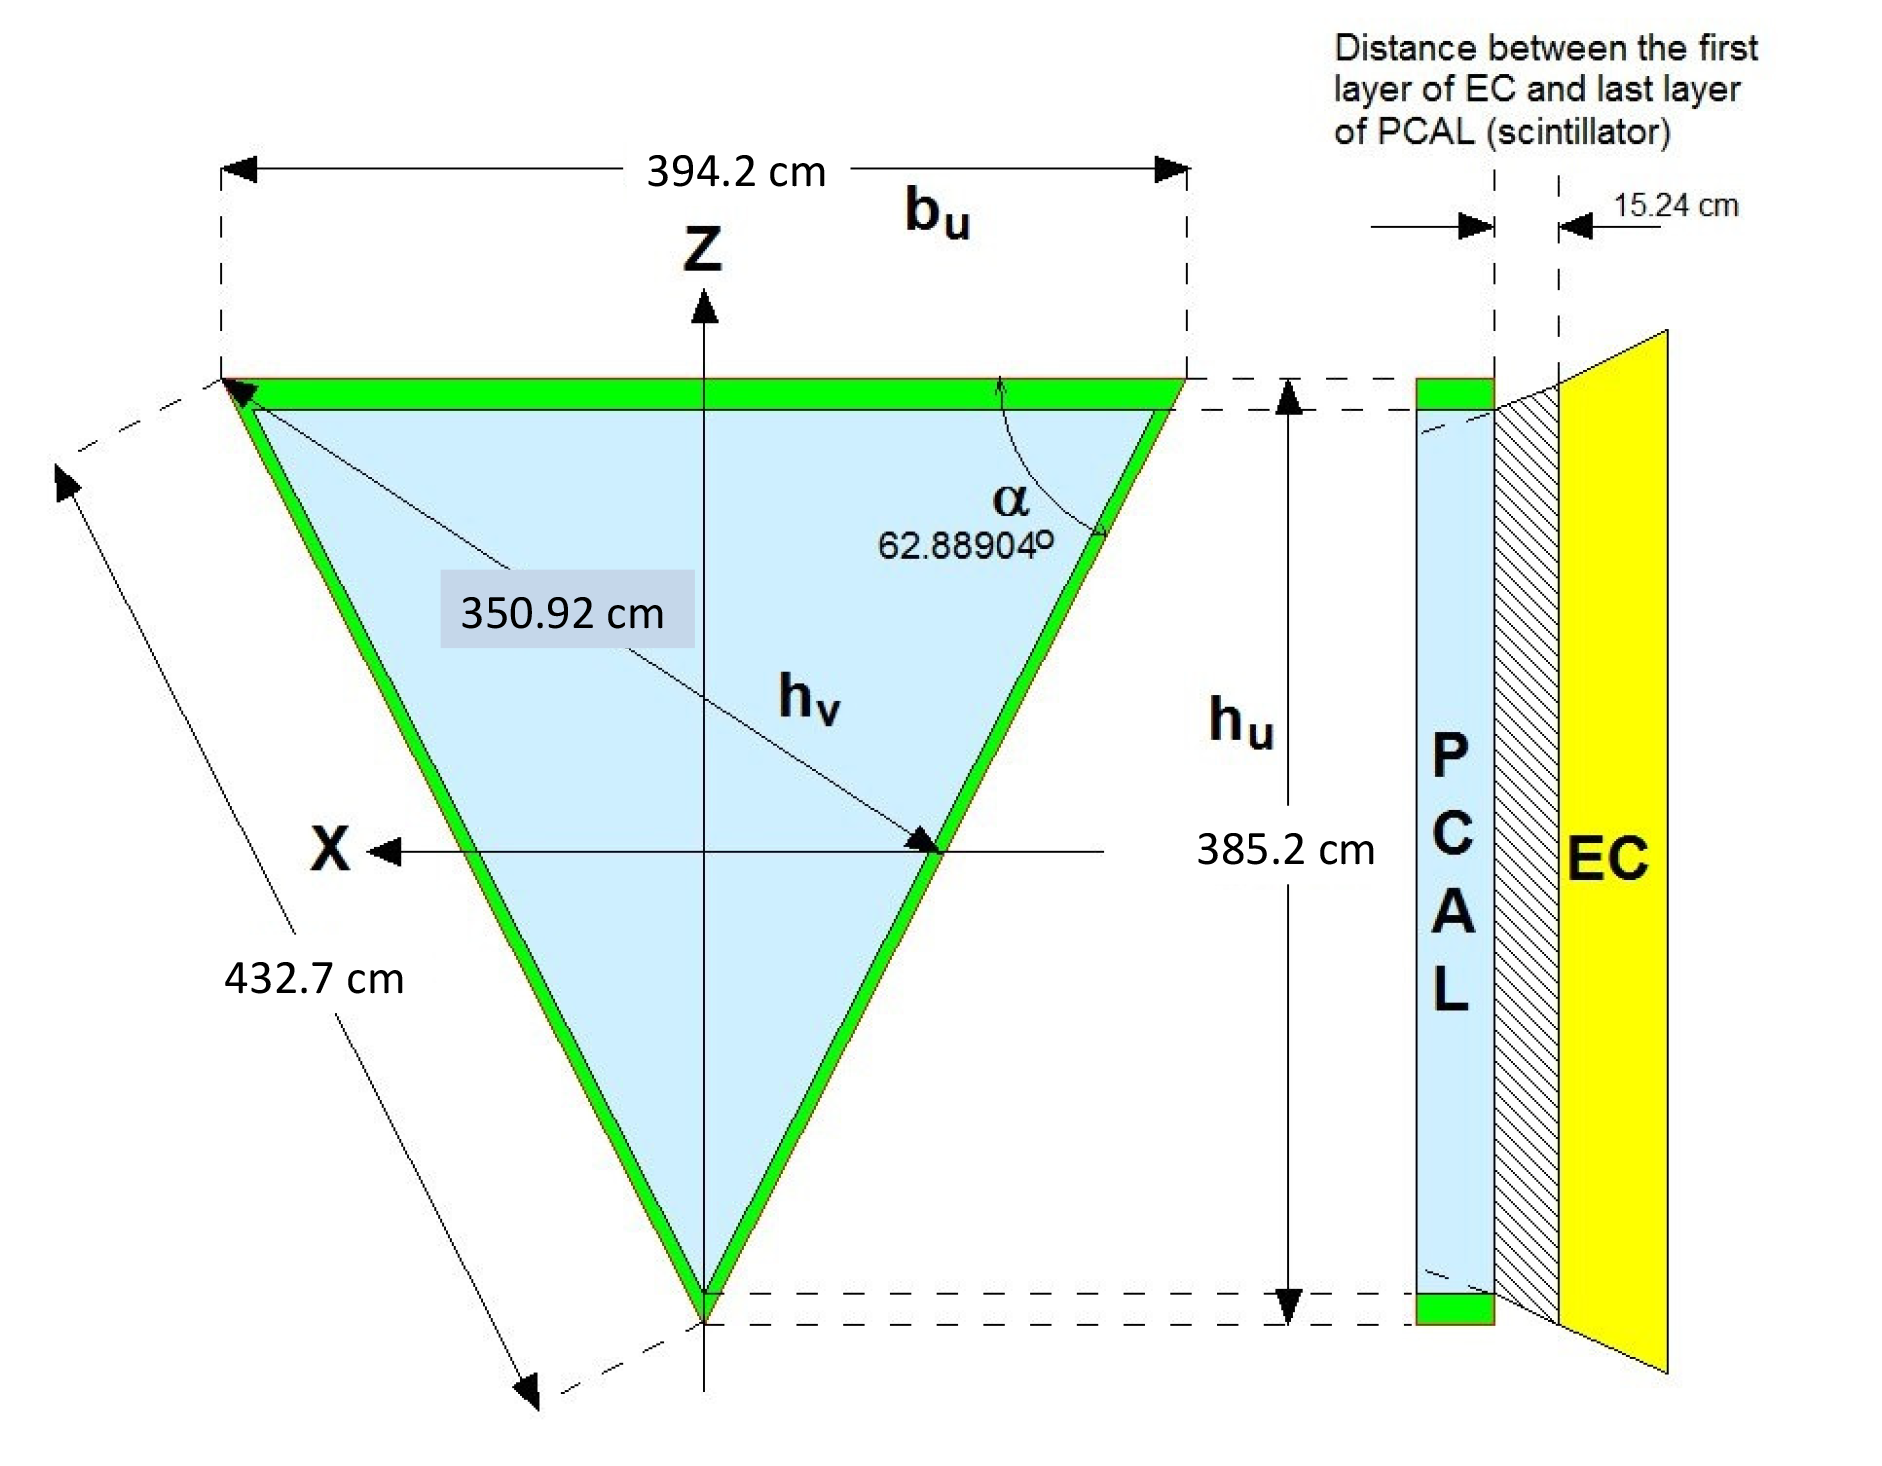
\includegraphics[width= 5in, keepaspectratio = true]{Pcal_geom_fig1}
    \caption{This diagram demonstrates the dimensions of the PCAL unit. This figure has been taken directly from the PCAL 
    geometry note\cite{bib:geomnote}.}
    \label{fig:geomfig1}
\end{figure}

The PCAL box encapsulates layers of scintillator strips and lead sheets. Between each lead sheet there are three different 
orientations of scintillating strips. These orientations are described as the U, V, and V layers. Each layer is parallel 
with one side of the PCAL box. The sequencing of the lead sheet, U layer, V layer, and W layer is repeated five times within
each sector of the PCAL unit. This results in fifteen layers of scintillator strips. Each repeating layer signal is coupled 
to the same PMT, and  is not able to separate five different signals. A UVW view of the PCAL can be seen in Fig.~\ref{fig:geomfig5}.

\begin{figure}[h]
    \centering
    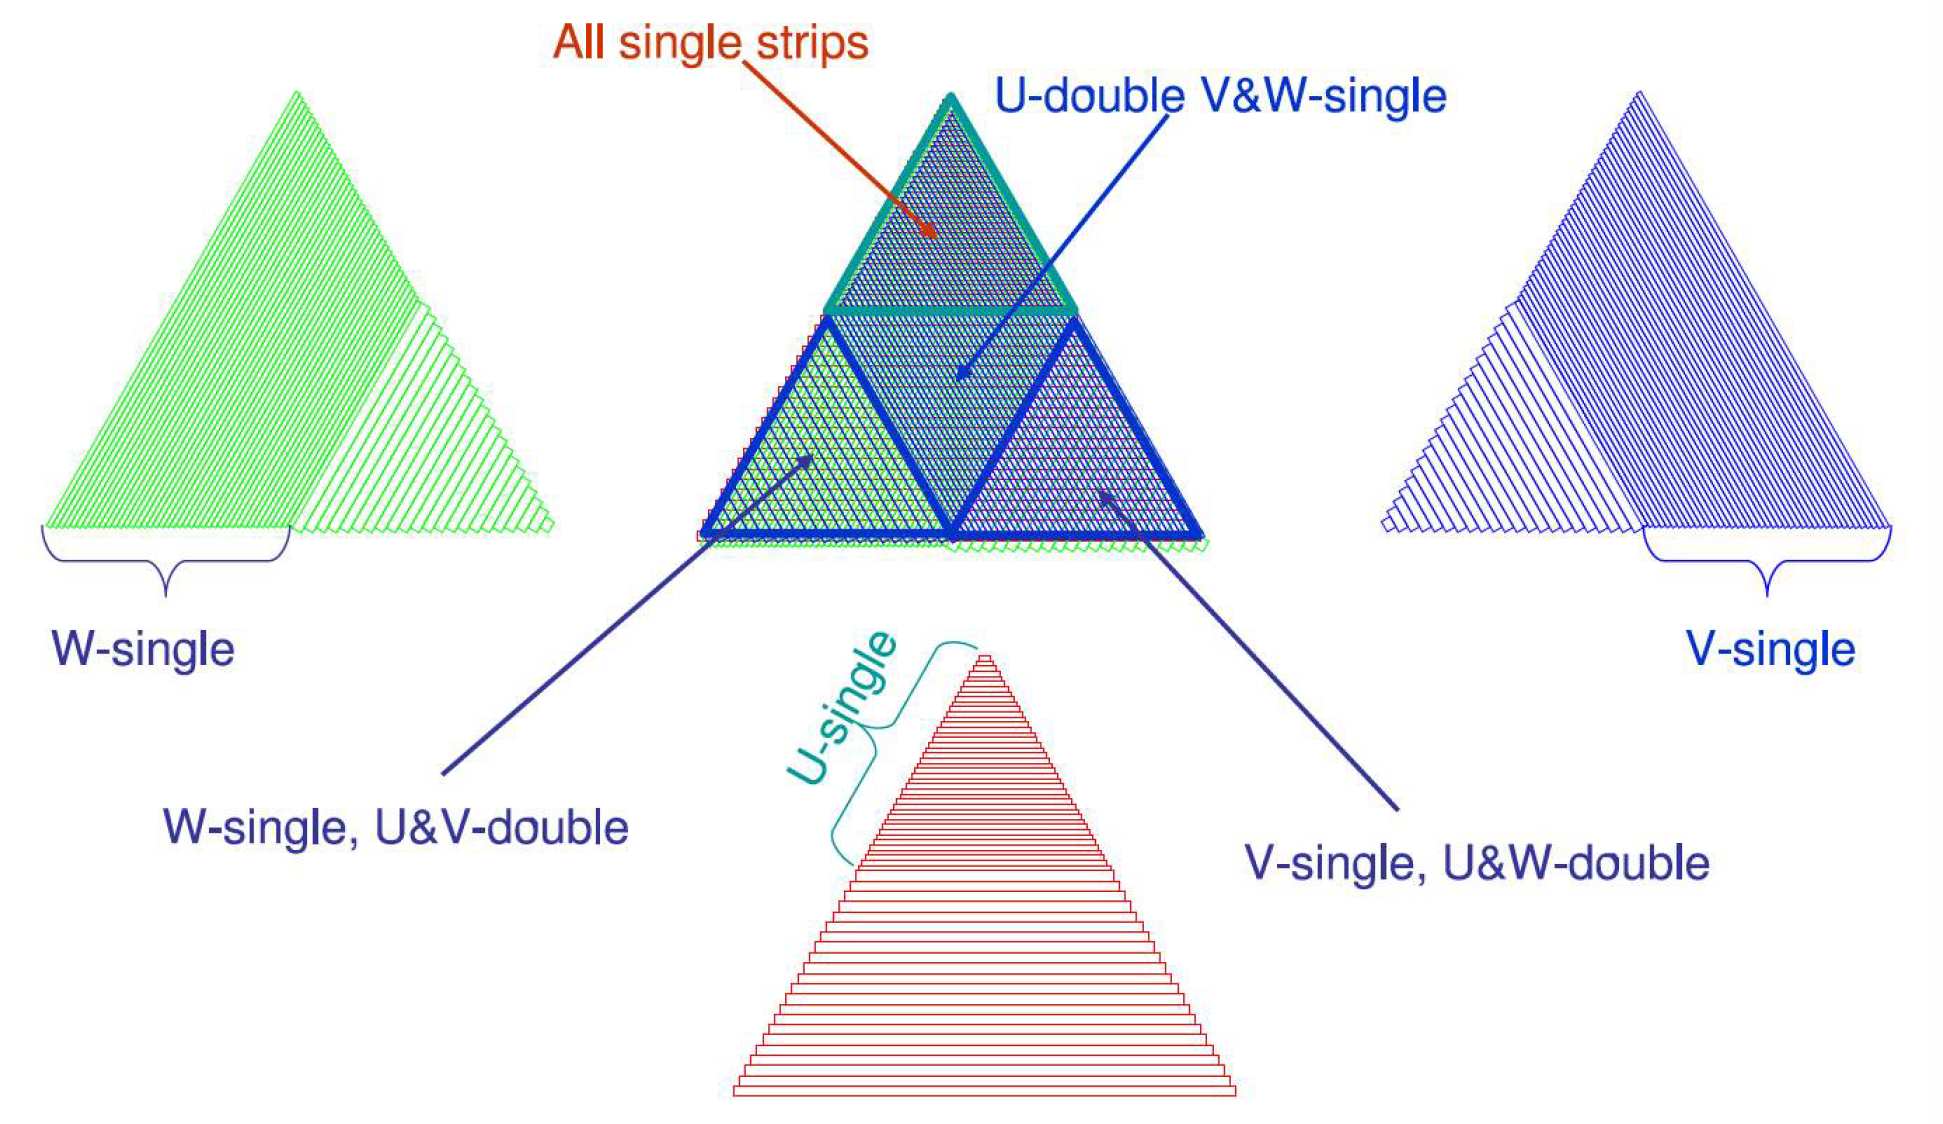
\includegraphics[width= 5in, keepaspectratio = true]{Pcal_geom_fig5}
    \caption{This is a schematic of how each orientation of scintillator is laid out. This figure is also taken directly from
     the PCAL geometry note\cite{bib:geomnote}.}
    \label{fig:geomfig5}
\end{figure}
\FloatBarrier

\FloatBarrier
There are 84 U strips, 77 V strips, and 77 W strips in each corresponding layer. The last 32 U strips are grouped into one PMT
per pair. The first 30 V and W strips are also grouped in pairs within their respective layer. As a consequence 
there is better spatial resolution at low strip numbers in the U layer and at high numbers in the V and W layers. This pattern 
of scintillators can be seen in Fig.~\ref{fig:geomfig5}.

Strips in each view can be numbered for ease. Lower numbered strips are the smaller strips while higher numbered strips are longer.
For example, V1 is the shortest and V62 is the longest strip in the V view. This strip convention is used throughout this
document and is taken from the PCAL geometry note\cite{bib:geomnote}. Using this convention, the layout of the PMT readout 
can easily be understood from Fig.~\ref{fig:PMTreadout} which shows PMT readout of a strip in each view. \textcolor{red}{The 
current analysis extracts calibration information based on 2-strip pixels only.}

\begin{figure}[h]
    \centering
    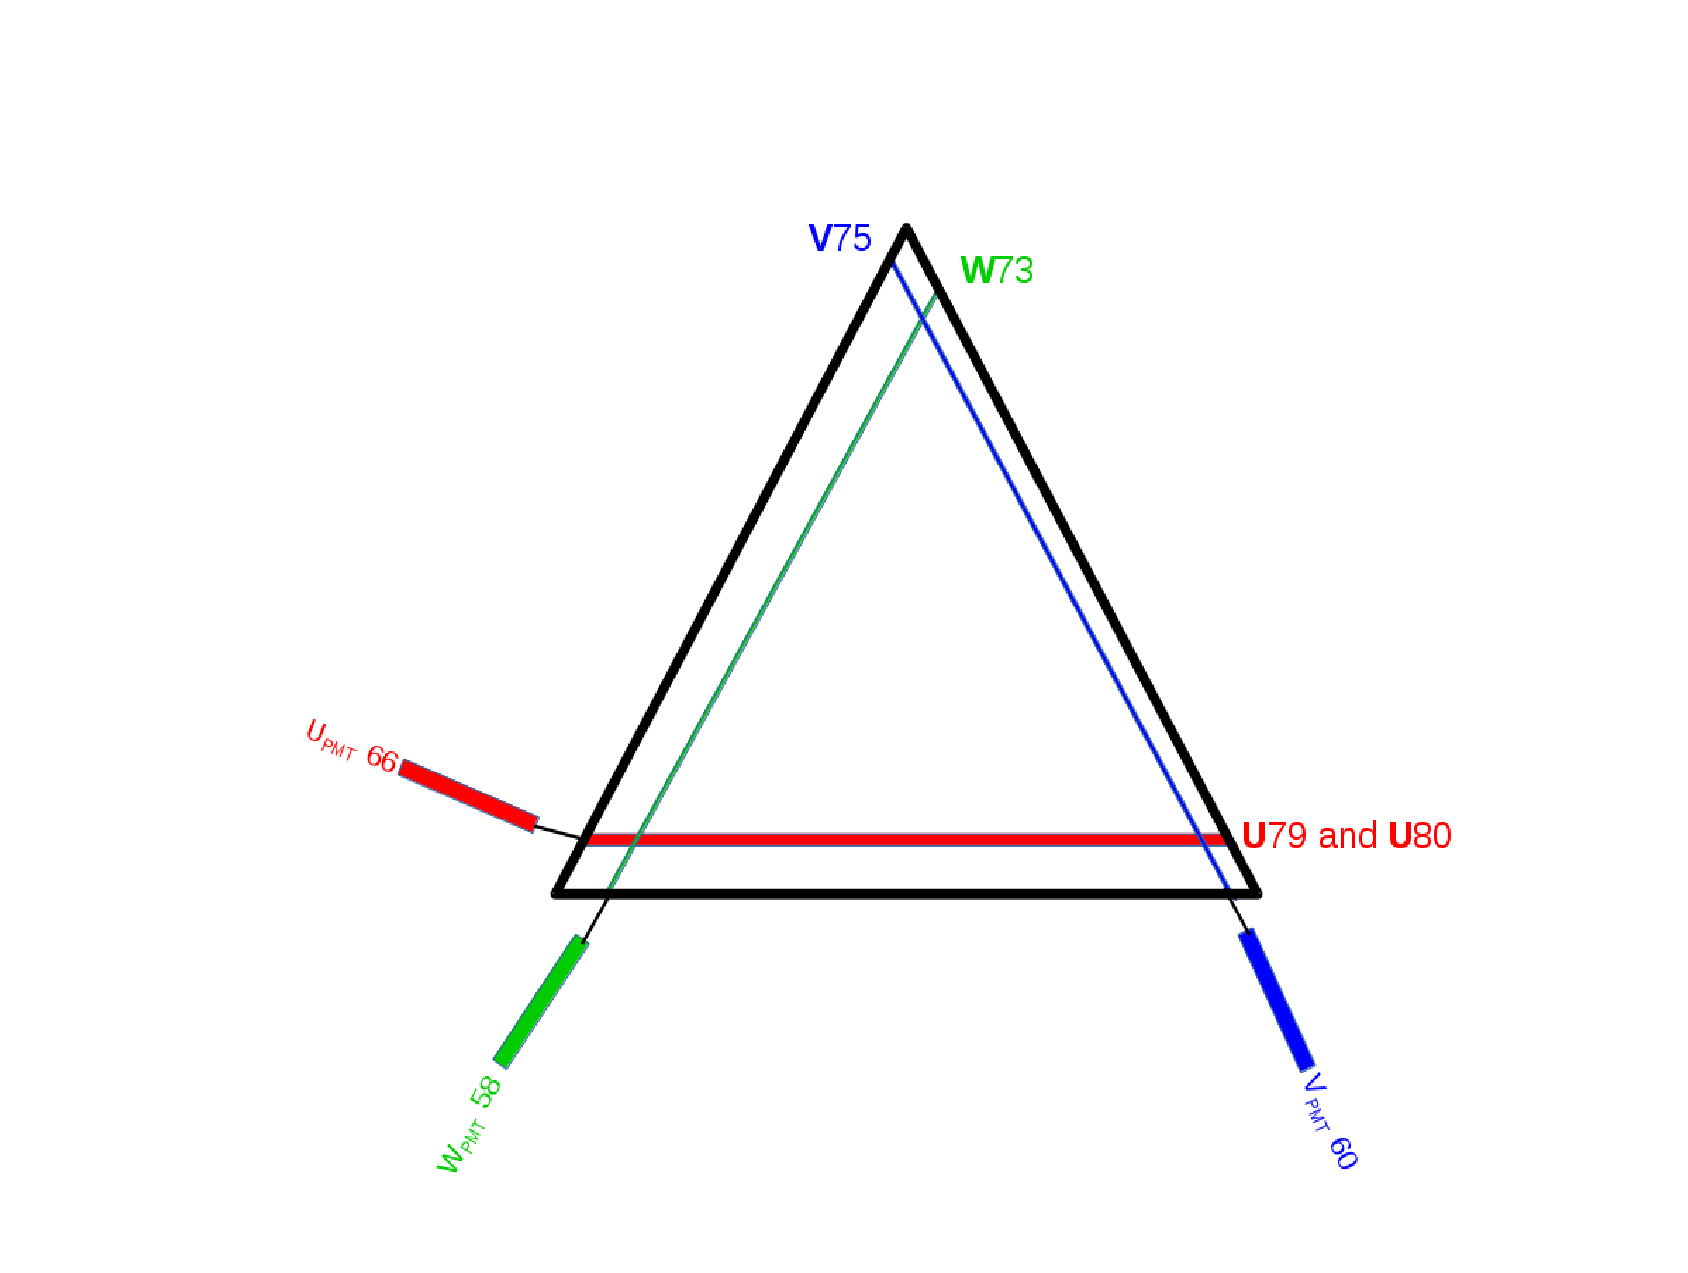
\includegraphics[width= 4.5in, keepaspectratio = true]{PMTreadout}
    \caption{This is a cartoon showing the layout of the PMT readout for different views.}
    \label{fig:PMTreadout}
\end{figure}
\FloatBarrier

\FloatBarrier
\subsection{Overlapping Shapes}
In order to calibrate the PCAL unit of the CLAS12 detector, one can think of dividing each PCAL module into bins based on the 
overlapping shapes. The overlap shapes/pixels are of two types: a 3-strip pixel, shape formed when all 
all the views are superimposed together, and a 2-strip pixel formed from the overlap of two strips where the strips are
part of different views. Maps of different overlap conditions are shown in Fig.~\ref{fig:PCAL_overlap}.


\begin{figure}[h]
  \centering
  \begin{subfigure}[b]{0.45\textwidth}
  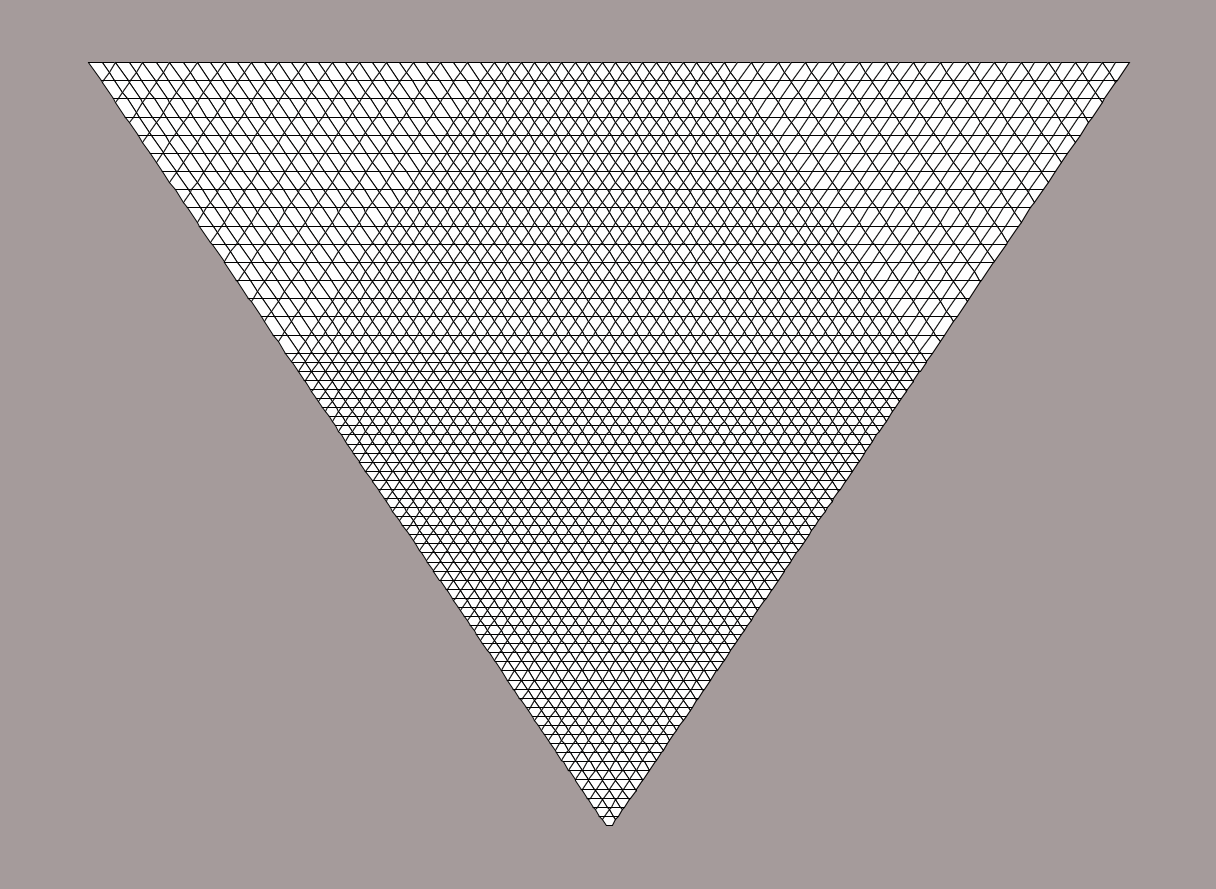
\includegraphics[width= 3in, keepaspectratio = true]{PCAL_pixel_screenshot}
  \caption{Pixel map.}
  %\label{fig:PCAL_pixel_screenshot}
  \end{subfigure}
  ~
  \begin{subfigure}[b]{0.45\textwidth}
  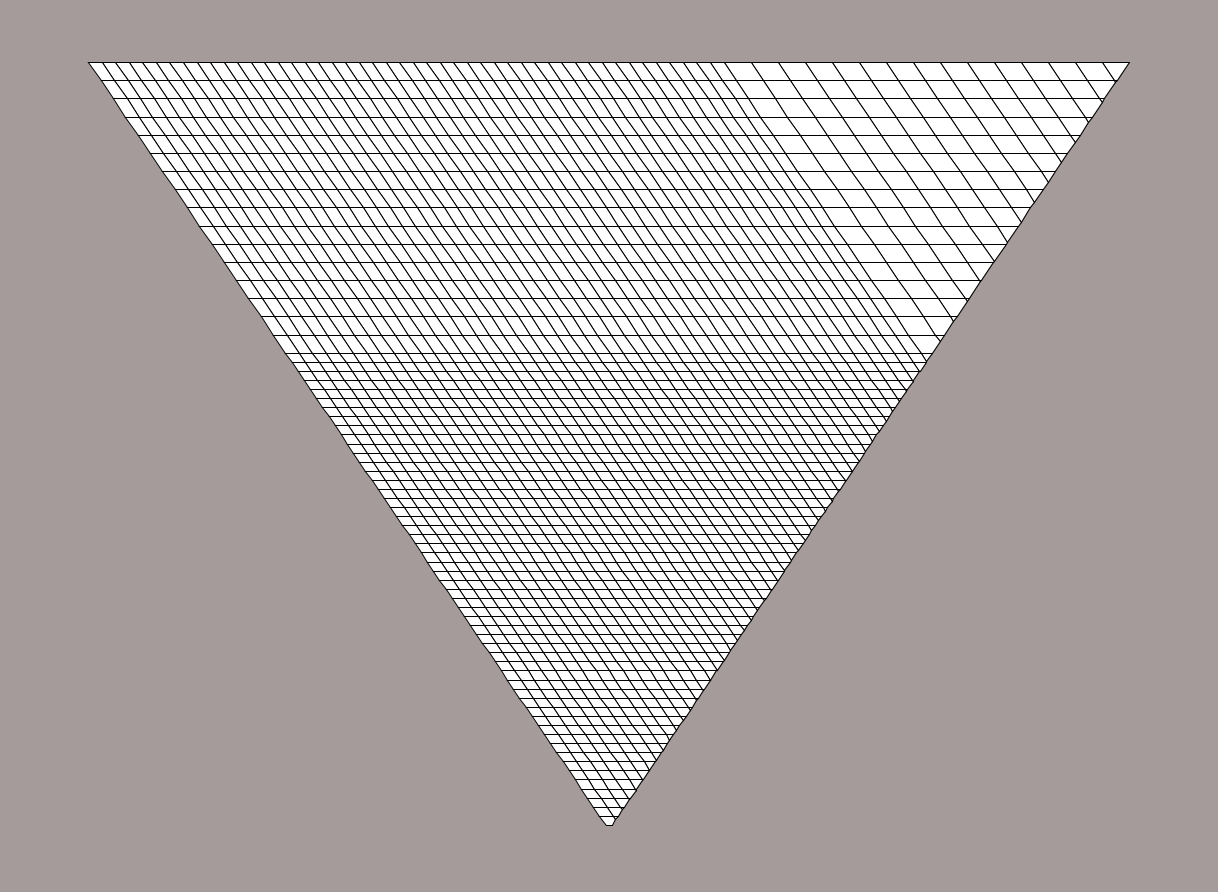
\includegraphics[width= 3in, keepaspectratio = true]{PCAL_UW_screenshot}
  %\caption{$M_{\pi^{+}\pi^{-}}$}
  %\label{fig:geomfig3b}
  \caption{UW overlap map.}
  %\label{fig:PCAL_UW_screenshot}
  \end{subfigure}

  \begin{subfigure}[b]{0.45\textwidth}
  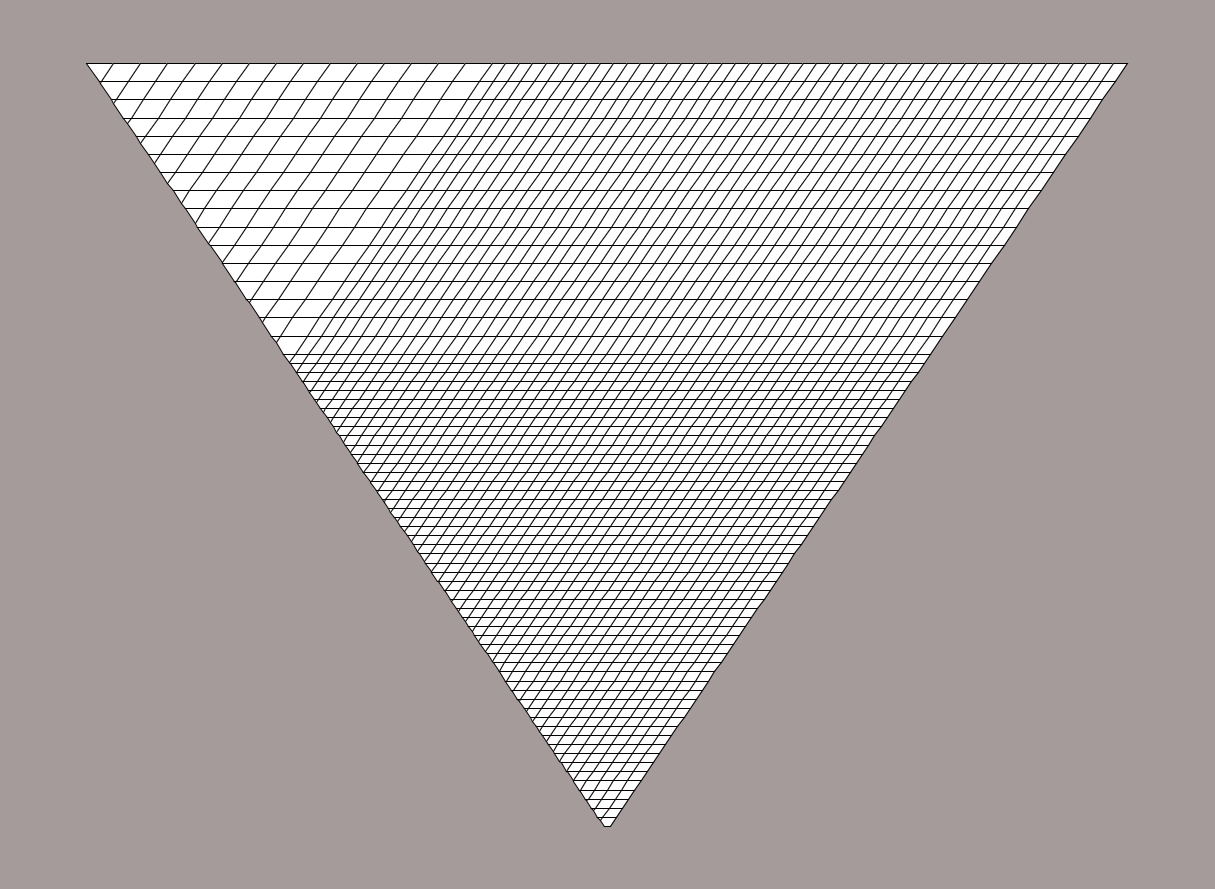
\includegraphics[width= 3in, keepaspectratio = true]{PCAL_UV_screenshot}
  %\caption{$M_{\pi^{+}\pi^{-}}$}
  %\label{fig:geomfig3b}
  \caption{UV overlap map.}
  %\label{fig:PCAL_UV_screenshot}
 \end{subfigure}
  ~
  \begin{subfigure}[b]{0.45\textwidth}
  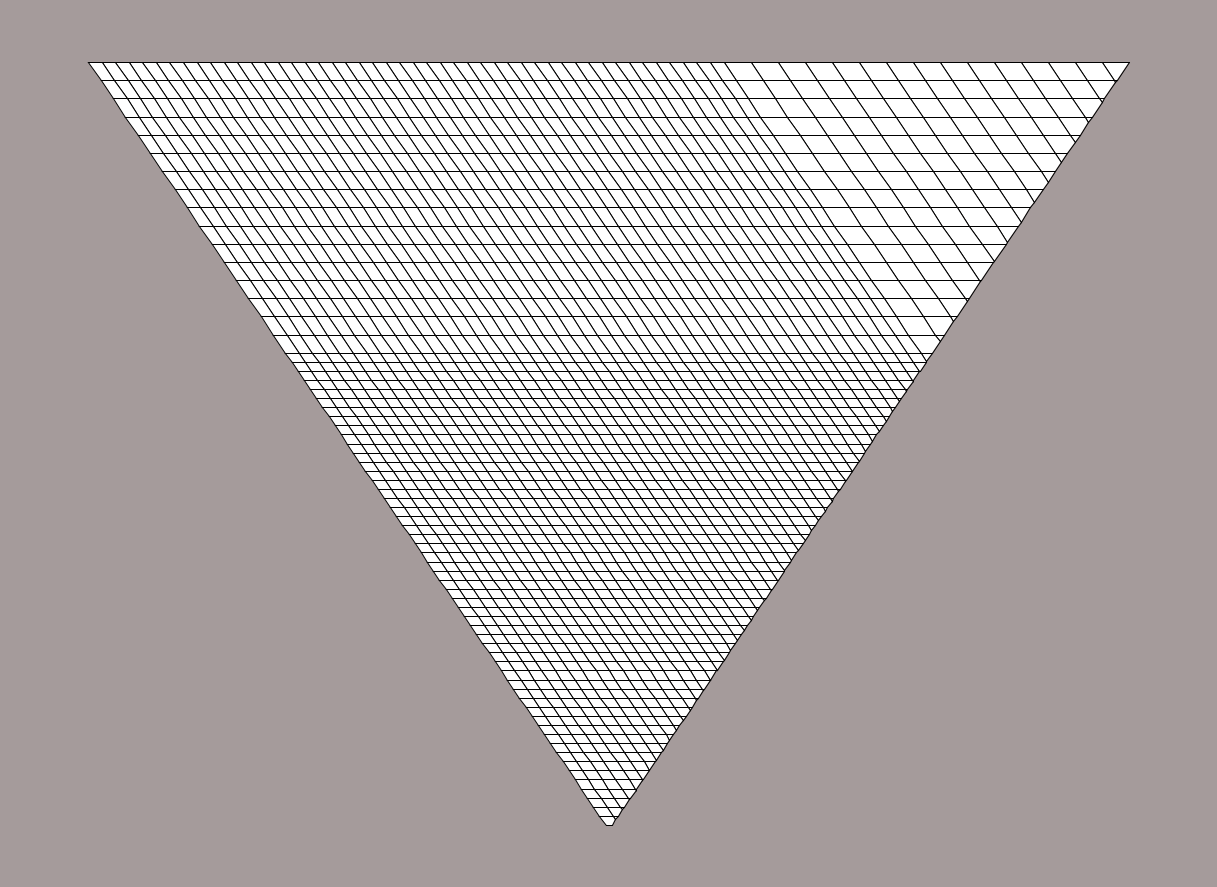
\includegraphics[width= 3in, keepaspectratio = true]{PCAL_WU_screenshot}
  \caption{WU overlap map.}
  %\label{fig:PCAL_WU_screenshot}
  \end{subfigure}
  ~
  \caption{Shown are the different ways overlaps can be considered in a single PCAL module.}
  \label{fig:PCAL_overlap}
\end{figure}
\FloatBarrier

\section{Data and Simulation}
The data used for the calibration was collected for the cosmic ray events before the PCAL unit was installed as a part of the CLAS12
detector subsystem. The collection required a trigger on the W-view meaning that information of cosmic ray tracks that created a PMT pulse of certain 
height were only stored. As the W-view is the last of the views, this trigger would also ensure to a reasonable level that the tracks
were perpendicular to the unit.

The calibration constants are extracted from simulated events as well to check the consistency of calibration code (based on \texttt{C++})
and the method used for the data. A \texttt{JAVA} framework is used for simulation and eventually the data. Details about the generation of 
simulated events and attenuation coefficients' extraction can be found in Section~\ref{Sec:simulation}.
\clearpage


%\section{Overlap Analysis}
In order to calibrate the PCAL unit of the CLAS12 detector, one can think of dividing each PCAL module based on the 
overlapping shapes. One can either consider on the pixel level, where the pixel is a shape formed when all 
all the views are superimposed together or the calibration can be done by considering the strips of one 
view binned in the number of strips in the view which is to be calibrated. Although in general a three layer 
correlated pixel can be odd shaped, a two layer correlation can be straight forward. This section deals with the 
latter case. The general idea is to get the ADC readout pertaining to that overlap shape which is at a certain 
distance from the PMT corresponding to the strip for that particular view. These signals are fit to extract the 
centroids which are further fit as an exponential function of distance to get the calibration coefficients 
or the attenuation coefficients. 

\FloatBarrier
\subsection{Overlap Distance Measurement}
An important parameter in the calibration process is the measurement of distances of the overlap shapes. 
As previously mentioned, the distances are measured from the PMTs. Therefore from the known width of each 
scintillator strip and the number of strips in between an overlap shape and the readout end, it is 
straightforward to calculate the distances for each overlap shape by simple trigonometry. This idea, 
however, assumes that all the strips are of equal width and neglects any physical gap (if any) between strips.

The two layer correlation creates trapezoidal bins formed by the overlap of two different 
strip orientations\footnote{All of the studies in this section were primarily focused on the U-strip 
attenuations, rather than the V or W strips.}. An example of one of these trapezoids outlined in black can be 
seen in figure \ref{fig:trapezoidUWintersection}. Each one of these trapezoids should have a ADC readout value. The width 
of this physical bin can be found by
\begin{eqnarray}
 s = \frac{w}{\sin{\alpha}}    \nonumber\\
\Rightarrow s = \frac{w}{\cos{\beta}},
\end{eqnarray}
where $w$ is a single scintillator strip width ($\approx 4.5$cm) and $\alpha = 62.88904^0$. Statistically one might expect some 
sort of peak describing the distribution of values. The centroid of this distribution is used as a data point 
at that center of that physical bin.
\begin{figure}[t]
\centering
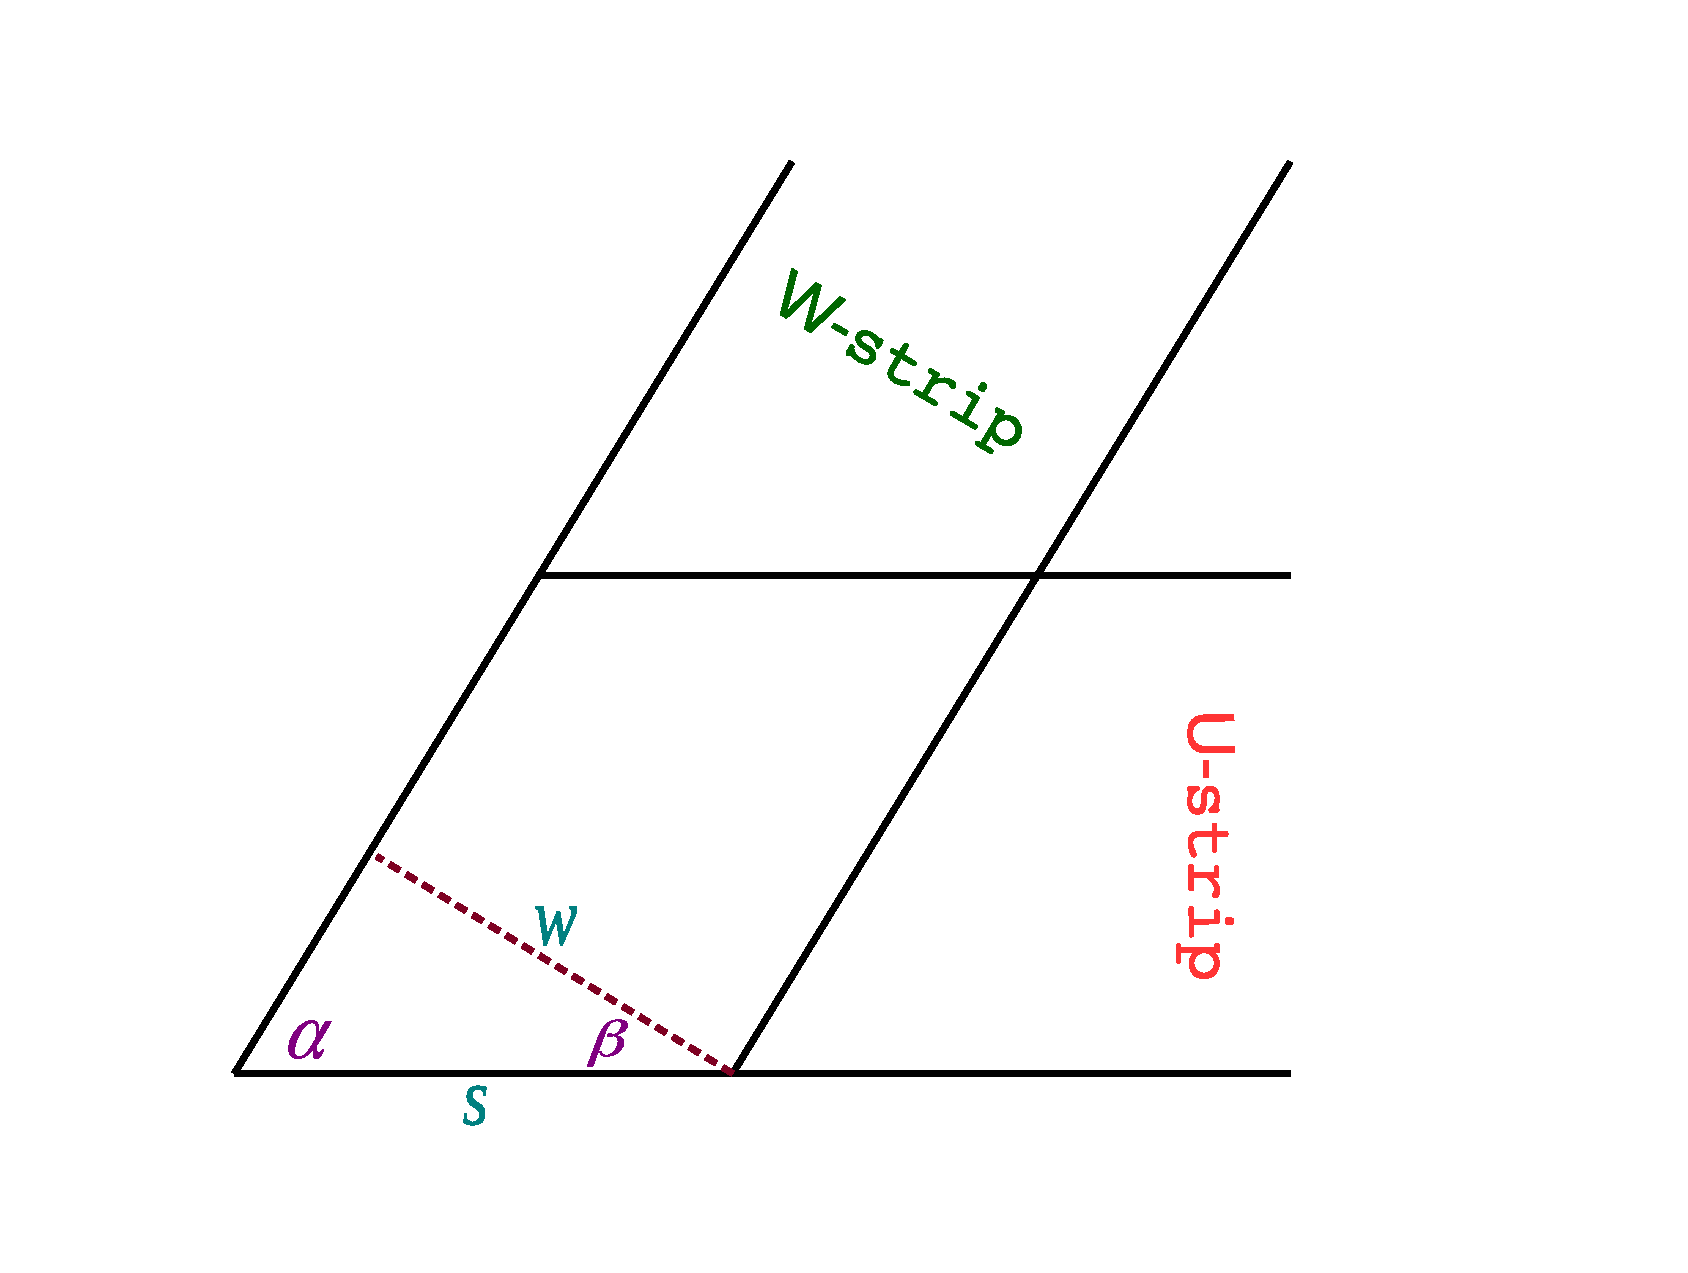
\includegraphics[width= 4in, keepaspectratio = true]{trapezoidUWintersection}
\caption{Shown is an outline of a generic intersection of a U and W strip. The distance between the trapezoidal area and the 
PCAL edge can be represented by a linear function of $s$.}
\label{fig:trapezoidUWintersection}
\end{figure}
\FloatBarrier

\clearpage


\section{Event Selection}

Triggers selected for calibration are restricted to events where only a single pixel is hit by the cosmic muon.  This ensures the muon trajectory is nearly perpendicular and does not undergo multiple scattering.  As a result a uniform distribution of desposited MIP energy is seen by all the PMTs, which provides a more accurate calibration. An intitial skim was used to select events that are most likely to involve a single pixel hit, using a multiplicity cut and a geometrical constraint.

\FloatBarrier
\subsection{Multiplicity Cut}
The multiplicity cut removed any event that contained more than three PMT readouts (one from each layer). This reduces the number of cosmic ray events that are not perpendicular to the face of the PCAL unit.  If a cosmic ray trajectory is not perpendicular to the PCAL face, it can intercept multiple strips in one orientation (e.g. - strip U30 and U31 both receive a signal). Although the accepted range of non-perpendicular angles depends on the size of the strips and their overlapping shape, this effect is expect to average out.  This multiplicity cut also helps to remove events where multiple cosmic rays hit the detector within the same time interval.  Overall this cut removes 95\% of the triggered events. 

\FloatBarrier
\subsection{Dalitz Cut} 
The Dalitz cut relies on the geometry axiom that for any point inside an equilateral triangle, the sum of the distances to each edge of the triangle is constant.  The same result also applies to distances along the edge of the triangle, in which case the constant is equal to two.  Thus only PMT numbers are needed to test the Dalitz cut, rather than calculating the interior x and y coordinate for every hit.  Once the N=3 multiplicity cut is passed, only the Dalitz condition need be tested for the U,V,W combination of hit strips to ensure the combination arises from a single pixel. If this condition is not satisfied, then the hit recorded is most likely electronic noise, an indirect hit, or multiple cosmic ray hits recorded at once.

The relatively simple calculation is given by equations \ref{eq:udist}-\ref{eq:totaldist}.  The calculation uses normalized coordinates calculated from the number of the triggered PMTs, which compensates for the PCAL not being an equilateral triangle.  Examination of Figure \ref{fig:dalitz}~(left) shows that the N=3 multiplicity skim overwhelmingly favors events that produce a pixel, as indicated by the sharp peak at uvw=2 which contains most of the events.  An example of the kind of hit pattern that would cause events outside of the uvw=2 peak is shown in Figure \ref{fig:dalitz}~(right).

\begin{equation}
    dist(u) = \left\{
        \begin{array}{l l}
            u/84.0                       & \quad \text{if $u < 52$}\\
            (52.0 + (u - 52.0)\times2.0)/84.0 & \quad \text{if $u \geq 52$}
        \end{array} \right.{}
         \label{eq:udist}
\end{equation}

\begin{equation}
    dist(v) = \left\{
        \begin{array}{l l}
            2.0 \times v/77.0;                       & \quad \text{if $v < 15$}\\
            (30.0 + (v - 15.0))/77.0                 & \quad \text{if $v \geq 15$}
        \end{array} \right.{}
         \label{eq:vdist}
\end{equation}


\begin{equation}
    dist(w) = \left\{
        \begin{array}{l l}
            2.0 \times w/77.0;                       & \quad \text{if $w < 15$}\\
            (30.0 + (w - 15.0))/77.0                 & \quad \text{if $w \geq 15$}
        \end{array} \right.{}
         \label{eq:wdist}
\end{equation}


\begin{equation} 
    uvw = dist(u) +  dist(v) + dist(w)
    \label{eq:totaldist}
\end{equation}

\begin{figure}[h]
    \centering
    \begin{subfigure}[h]{0.44\textwidth}
        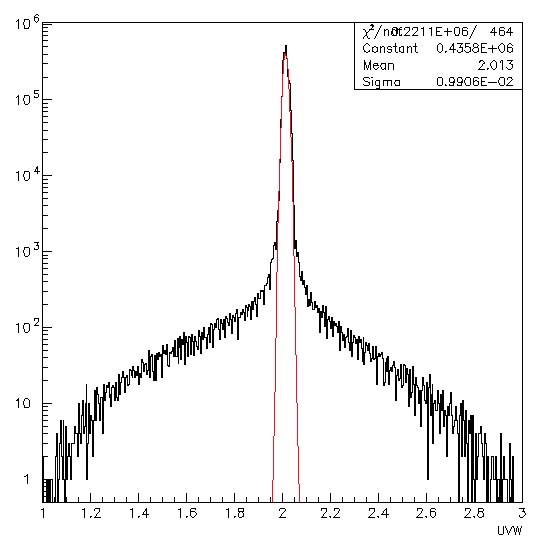
\includegraphics[height= 3in, keepaspectratio = true]{dalitz2}
        \label{fig:dalitz1}
    \end{subfigure}
    \begin{subfigure}[h]{0.55\textwidth}
        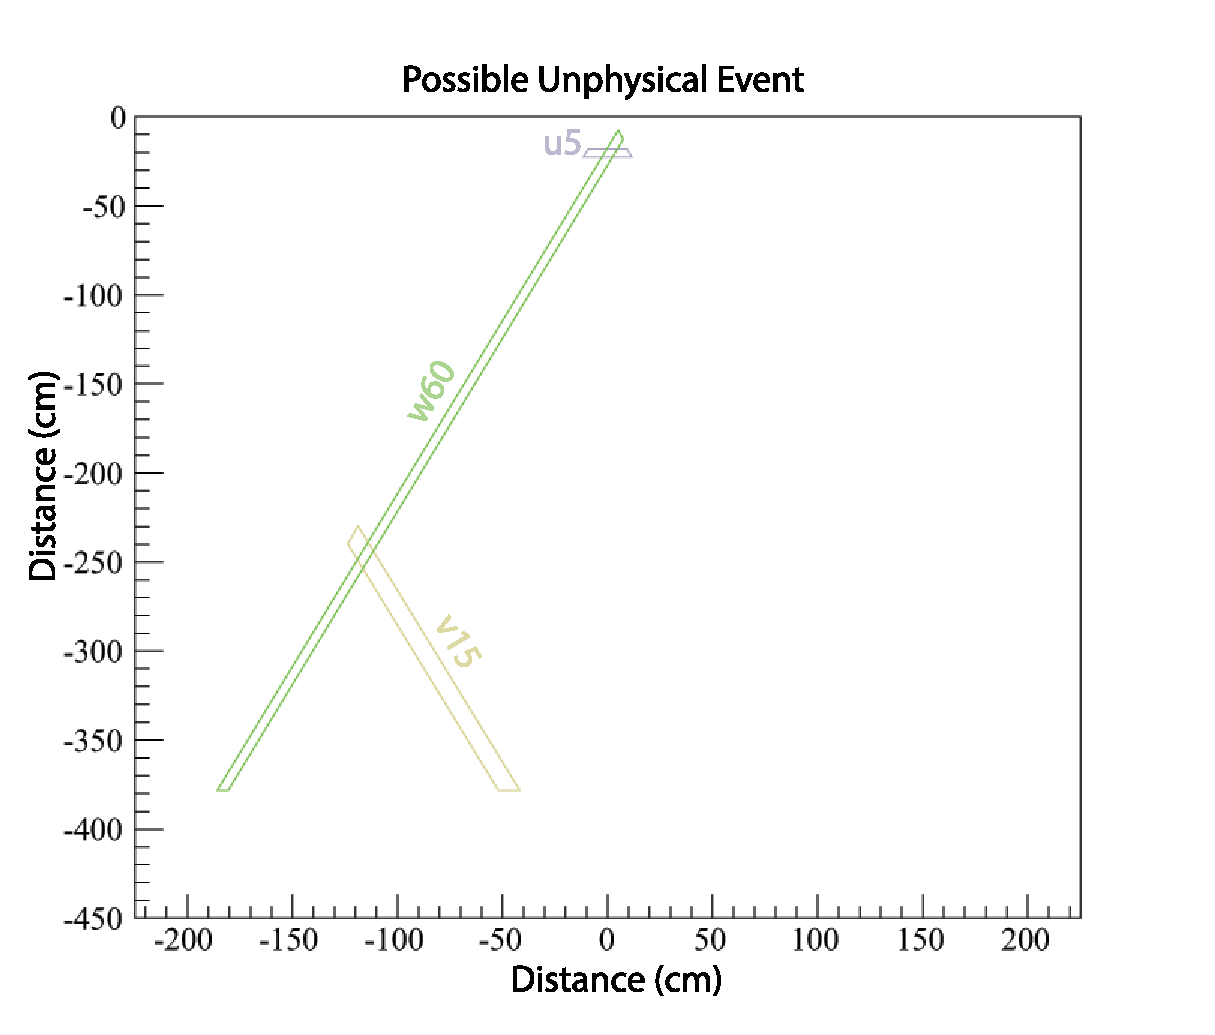
\includegraphics[height=3in, keepaspectratio = true]{unphysical}
        \label{fig:dalitz2}
    \end{subfigure}
\caption{LEFT: Histogram of Dalitz condition (\ref{eq:totaldist}) after multiplicity (N=3) skim of cosmic triggered data.\\ RIGHT: Example of an event that passed the N=3 cut, but fell outside of the Dalitz peak at uvw=2.}
\label{fig:dalitz}
\end{figure} 
\FloatBarrier


\section{Fit to ADC Output}
\label{Sec:fitToADCOutput}
Although in general a 3-strip pixel can be odd shaped, a 2-strip pixel can be straightforward. 
This two layer correlation creates trapezoidal bins formed by the overlap of two different strip 
orientations\footnote{All of the studies in this section were primarily focused on the u strip attenuations, 
rather than the v/w strips.}. An example of one of these trapezoids outlined in black can be seen in Fig.~\ref{fig:stripwidth}. 
Each one of these trapezoids should have a ADC readout value. The width of this physical bin can be found by

\begin{equation}
    s = \frac{w}{\sin{\alpha}}
    \label{eq:s}
\end{equation}
or
\begin{equation}
    s = \frac{w}{\cos{\beta}},
\end{equation}
where $w$ is a single scintillator strip width ($\approx 4.5$cm).
Statistically one might expect some sort of peak describing the distribution of values. The centroid of this 
distribution is used as a data point at that center of that physical bin.

\begin{figure}[h]
\centering
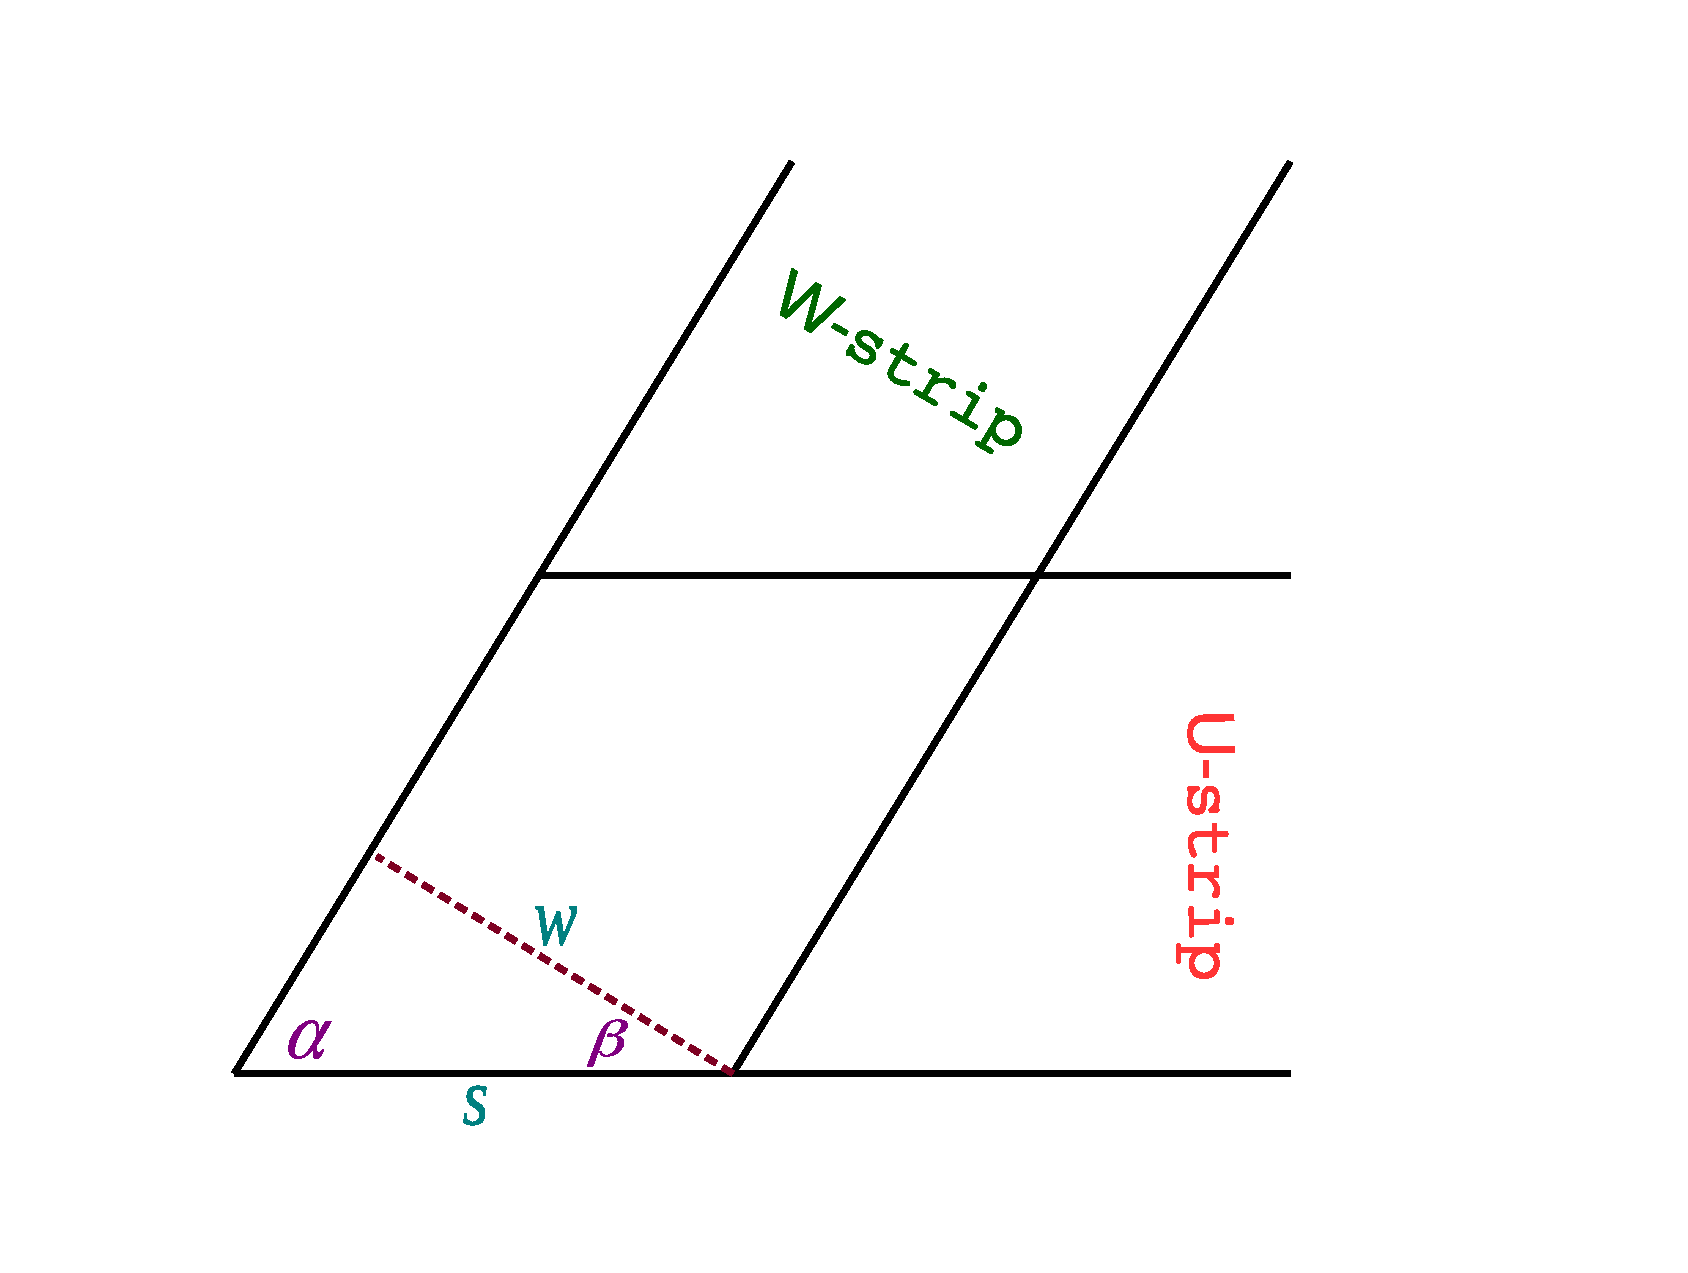
\includegraphics[width= 3in, keepaspectratio = true]{trapezoidUWintersection}%stripwidth
\caption{Shown is an outline of a generic intersection of a u and w strip. The distance between the trapezoidal
 area and the PCAL edge can be represented by a linear function of $s$.}
\label{fig:stripwidth}
\end{figure}

\FloatBarrier
\subsection{Signal Shape}
The desired outcome is to approximate the signal by a simple function, for instance a Gaussian function.
Upon investigation the integrated ADC values appear to be a combination of a Gaussian and exponential fits.

\begin{figure}[h]
    \centering
    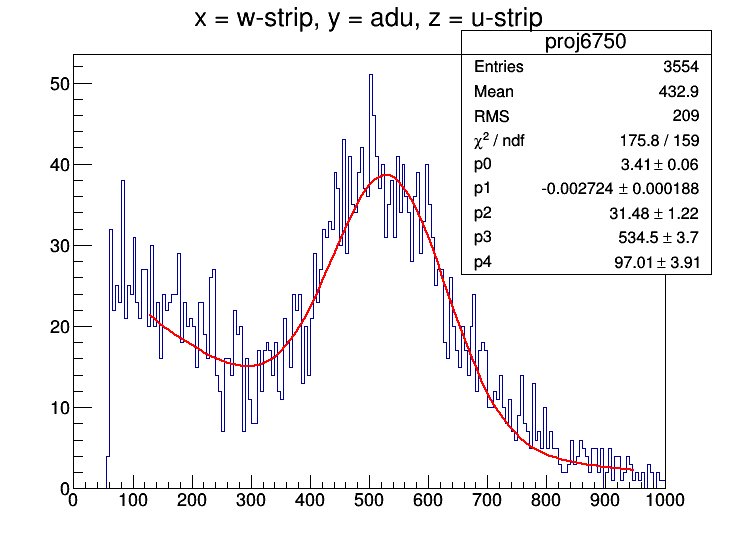
\includegraphics[width= 4in, keepaspectratio = true]{distribution}
    \caption{Shown is an example of the distribution of the ADC readout from one u/w trapezoidal bin 
    (specifically the logical numbers u =67, w=50). The red line is a fit to an exponential combined with 
    a Gaussian distribution.}
    \label{fig:distribution}
\end{figure}

This type of background can be seen for every physical two layered bin along any strip.

\begin{figure}[h]
    \centering
    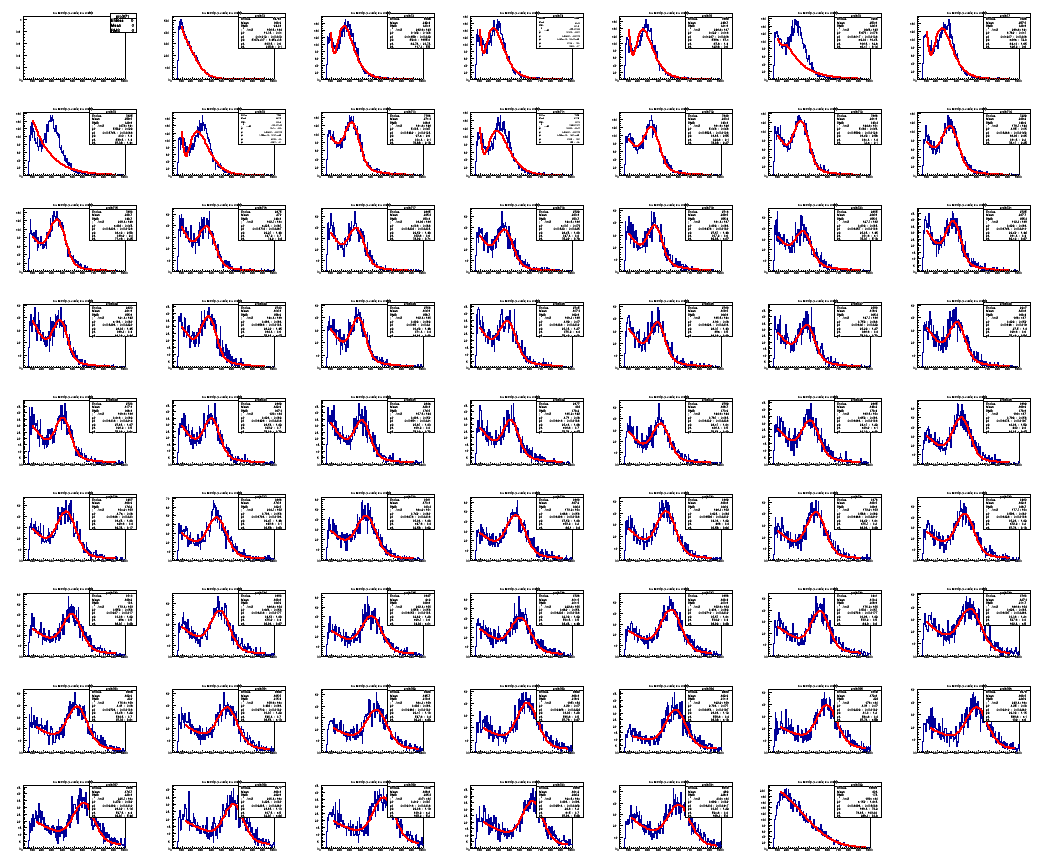
\includegraphics[width= 6in, keepaspectratio = true]{allstrip67}
    \caption{Shown is an example of all the distributions of the ADC readout from the 67th logical u strip.}
    \label{fig:allstrip67}
\end{figure}


\FloatBarrier
\subsubsection{Fit function}
Upon initial inspection the distribution is fit to an exponential and a Gaussian. 
The exponential is background/noise in most cases, whereas the Gaussian represents near perpendicular cosmic ray hits. 
The centroid of the Gaussian is extracted and determined to be the primary light intensity in that trapezoidal bin.

This plan works well for most interior physical bins. However, after looking at the strips corresponding to 
the edges of the PCAL unit, it is realized this can't be all that is done. Two possible improvements are 
utilized to better extend the calibration to the outer edges.

\begin{enumerate}
    \item Cut on each fit Gaussian signal. \\
        Using the fact that each bin in one scintillating strip corresponds to the other two, a cut on one 
        affects the others. By making an iteration over all events a three sigma cut can be placed on each
         signal. This reduces the exponential background. This improves the fits to some of the edges.
    \item Cut on the overall energy deposited. \\
        Assuming that the signal is from the same cosmic ray and if that event doesn't participate in 
        corner clipping, then the event should deposit the same amount of energy into each layer. After
         cutting on the original signal and fitting attenuation curves, individual gains can be 
         approximated. Using the emperically found gains, a cut on the sum of ADC signals can be 
         performed. This also helps the extend good fits to the edges of the pcal unit. This is 
         the case due to the fact that two intersecting medium range strips (other layers) set 
         limits on the possible events on the outer most strips. By improveing the outer most strips,
          they can be used to set limits on the overlapping shorter strips.  
\end{enumerate}

\FloatBarrier
\subsection{Iteration Process}
An iteration process was employed to improve the signal extraction. This process cuts events on
 ADC values determined by either the signal fits or by attenuation fits and then repeats. This 
 allows for a converging result because each cut on one layer affects the other two. Therefore
  the raw signal fit keeps improving as the attenuation fit and gains improve. To illustrate 
  how the process works, each iteration described in this section will describe cuts used when 
  plotting the raw signal. After the cuts are described an illustration of the fit to the signals 
  will be shown with a diverse sampling (as diverse as six options gets). Next an attenuation 
  fit over six of the strips will be shown. This shows how the multiple cuts affect each attenuation 
  fit as a function of strip number. 

\clearpage
\FloatBarrier
\subsubsection{Pass 0}
\begin{itemize}
    \item Multiplicity Cut: Only events where one PMT fired for each strip were allowed.
    \item Dalitz Cut: An empircal distance sum was used to remove events that don't fall into 
    this range determined by Equation \ref{eq:totaldist}.
    \item Valid hit or near neighbor hit: Using generated events on a calculated skeleton of 
    the pcal, each pixel was determined to be valid or not. Extra uncertainty was allowed by 
    also marking nearest neighboring pixels.
\end{itemize}

\begin{figure}[h]
    \centering
    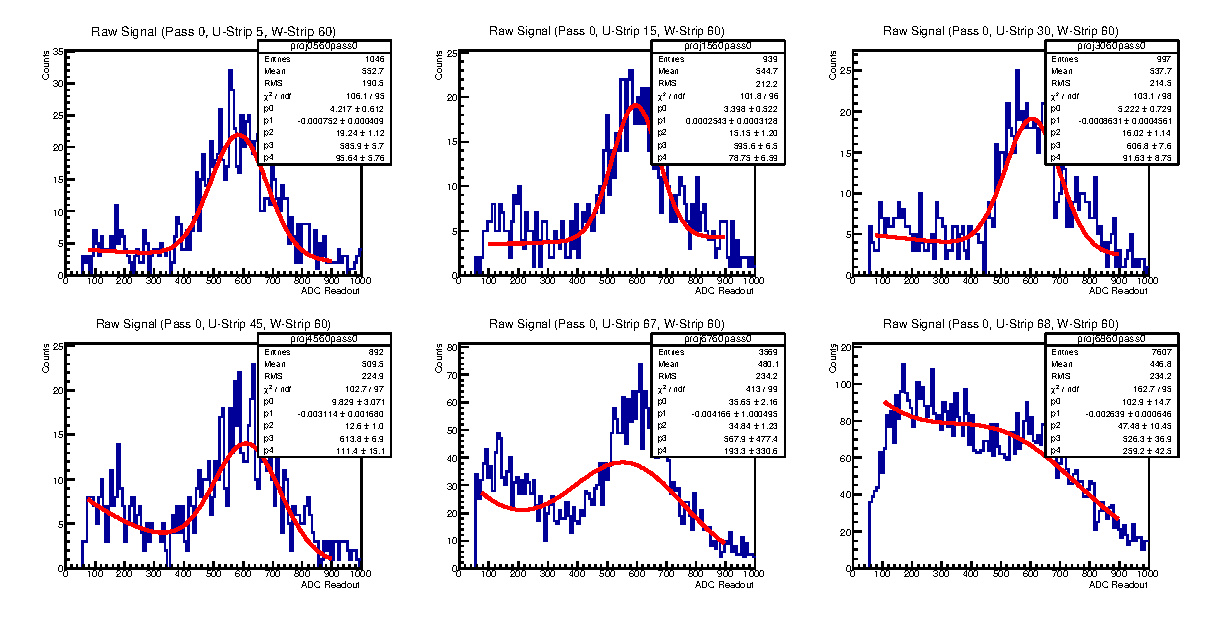
\includegraphics[height= 2.75in, keepaspectratio = true]{pass0}
    \caption{Shown is the ADC signal corresponding to signals from multiple u-strips 
    (5, 15, 30, 45, 67, and 68) and a projection of the w60 strip.}
    \label{fig:pass0}
\end{figure}

\begin{figure}[h]
    \centering
    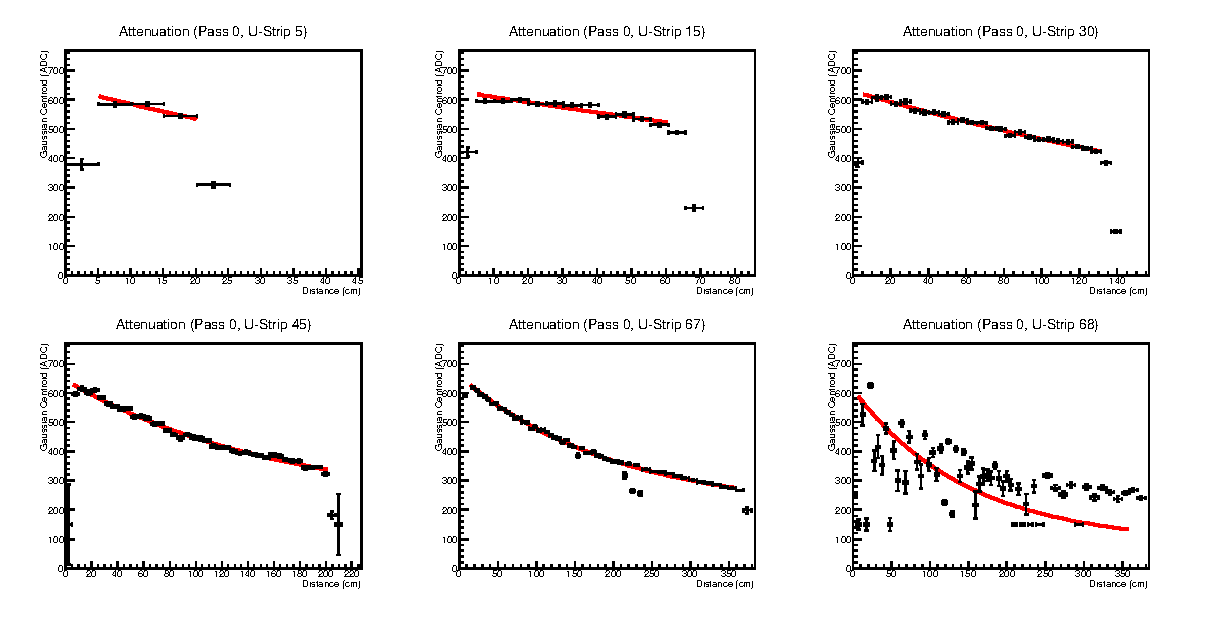
\includegraphics[height= 2.75in, keepaspectratio = true]{atpass0}
    \caption{Shown is the overall attenuation fits to the selected u-strips 
    (5, 15, 30, 45, 67, and 68).}
    \label{fig:atpass0}
\end{figure}


\clearpage
\FloatBarrier
\subsubsection{Pass 1}
\begin{itemize}
    \item Multiplicity Cut: Only events where one PMT fired for each strip were allowed.
    \item Dalitz Cut: An empircal distance sum was used to remove events that don't fall 
    into this range determined by Equation \ref{eq:totaldist}.
    \item Valid hit or near neighbor hit: Using generated events on a calculated skeleton
     of the pcal, each pixel was determined to be valid or not. Extra uncertainty was 
     allowed by also marking nearest neighboring pixels.
    \item 3$\sigma$ Cut on Signal: Each signal was fit to a Gaussian and exponential in 
    pass 0. The parameter $\sigma$ from the Gaussian fit was used to cut out the events
     that did not lie within this function.
\end{itemize}


\begin{figure}[h]
    \centering
    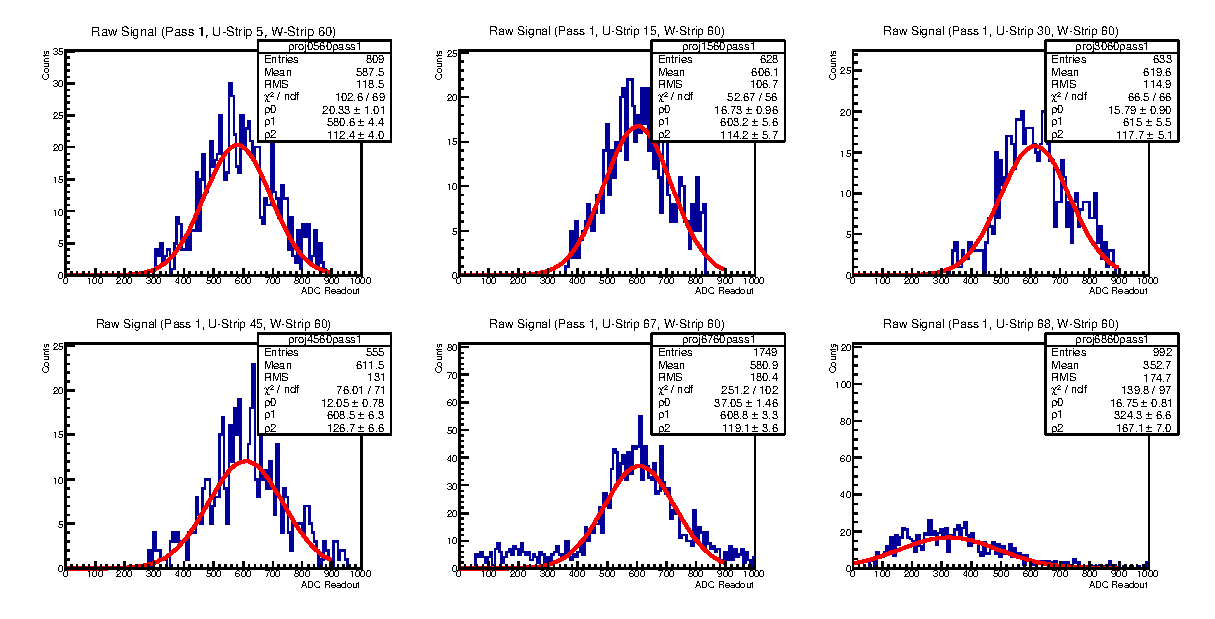
\includegraphics[height= 2.75in, keepaspectratio = true]{pass1}
    \caption{Shown is the ADC signal corresponding to signals from multiple u-strips
     (5, 15, 30, 45, 67, and 68) and a projection of the w60 strip.}
    \label{fig:pass1}
\end{figure}

\begin{figure}[h]
    \centering
    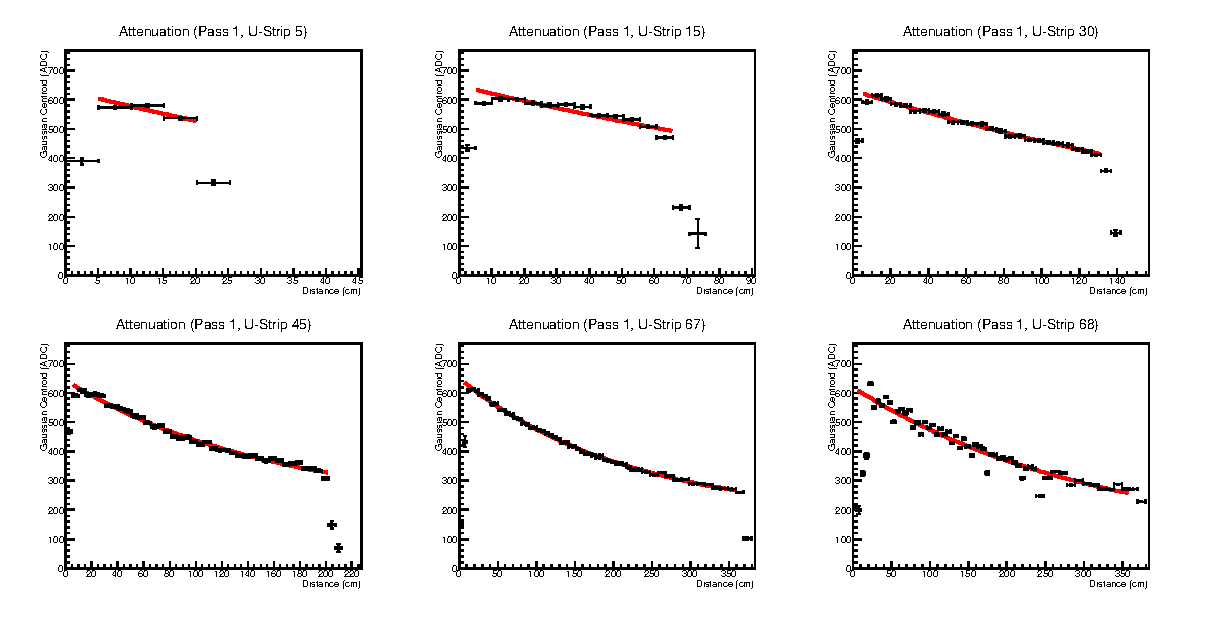
\includegraphics[height= 2.75in, keepaspectratio = true]{atpass1}
    \caption{Shown is the overall attenuation fits to the selected u-strips 
    (5, 15, 30, 45, 67, and 68).}
    \label{fig:atpass1}
\end{figure}



\clearpage
\FloatBarrier
\subsubsection{Pass 2}
\begin{itemize}
    \item Multiplicity Cut: Only events where one PMT fired for each strip were allowed.
    \item Dalitz Cut: An empircal distance sum was used to remove events that don't fall 
    into this range determined by Equation \ref{eq:totaldist}.
    \item Valid hit or near neighbor hit: Using generated events on a calculated skeleton 
    of the pcal, each pixel was determined to be valid or not. Extra uncertainty was allowed 
    by also marking nearest neighboring pixels.
    \item Cut on Attenuation Fits: When the signals where the Gaussian centroid from pass 1 
    were outside an ADC value of $\pm50$ from the attenuation fit, the obtained $\sigma$ was 
    ignored and a new cut about the attenuation fit was employed. If the centroid was close 
    to ADC value from the attenuation fit a 2$\sigma$ cut was used to remove extra background.
\end{itemize}


\begin{figure}[h]
    \centering
    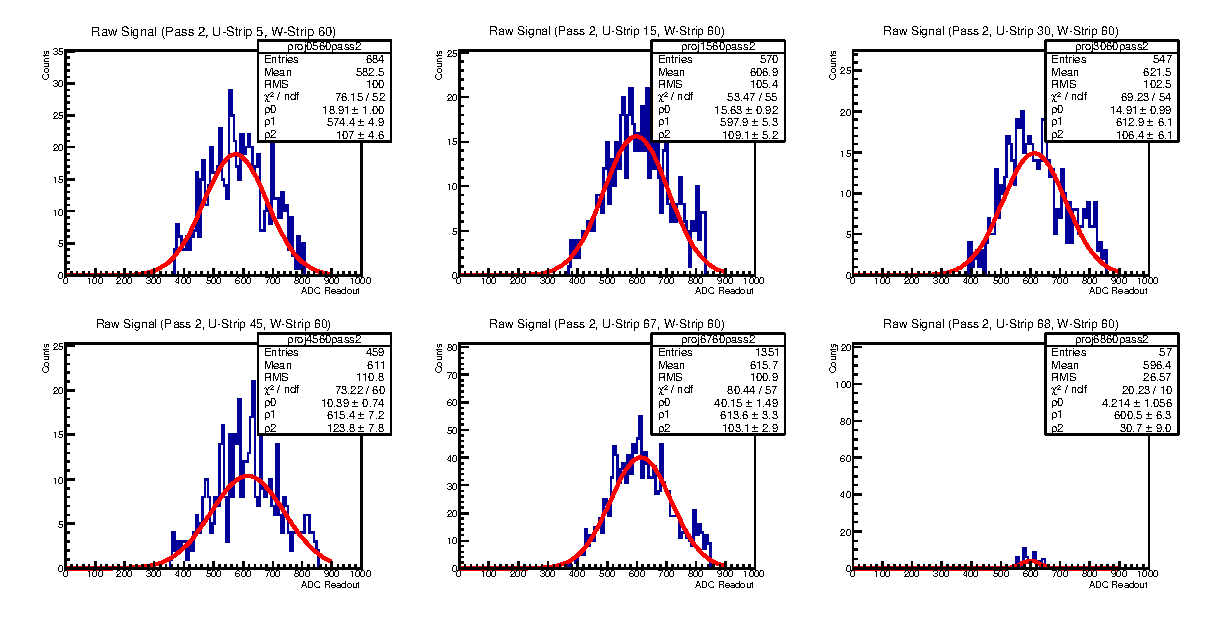
\includegraphics[height= 2.75in, keepaspectratio = true]{pass2}
    \caption{Shown is the ADC signal corresponding to signals from multiple u-strips 
    (5, 15, 30, 45, 67, and 68) and a projection of the w60 strip.}
    \label{fig:pass2}
\end{figure}

\begin{figure}[h]
    \centering
    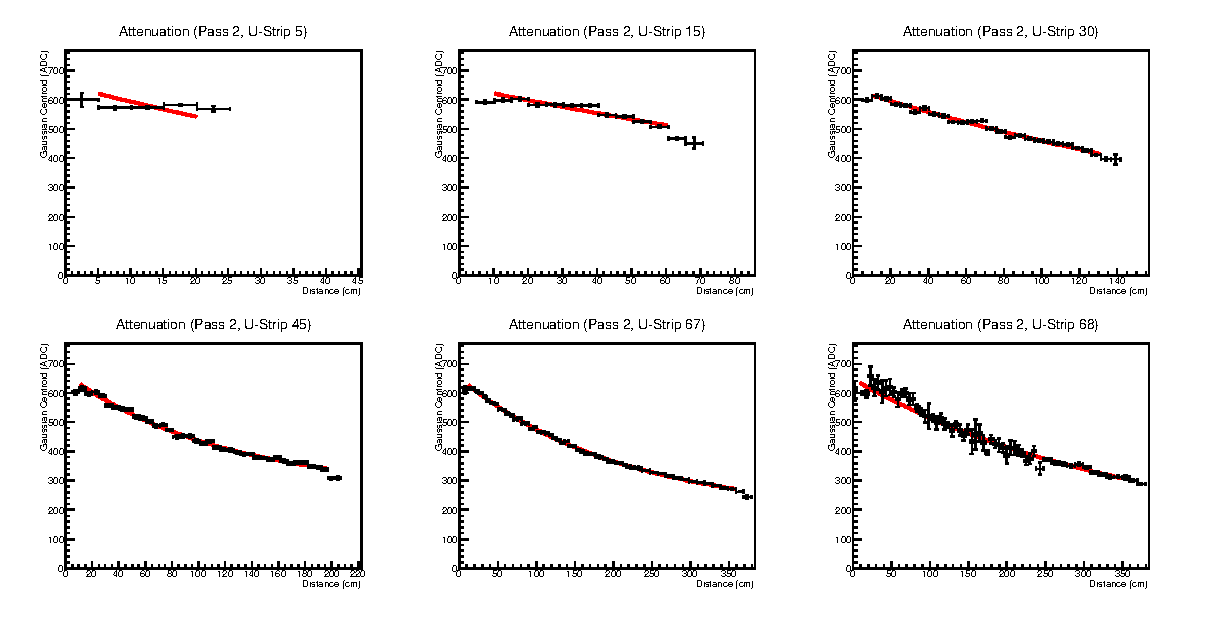
\includegraphics[height= 2.75in, keepaspectratio = true]{atpass2}
    \caption{Shown is the overall attenuation fits to the selected u-strips 
    (5, 15, 30, 45, 67, and 68).}
    \label{fig:atpass2}
\end{figure}



\clearpage
\FloatBarrier
\subsubsection{Pass 3}
\begin{itemize}
    \item Multiplicity Cut: Only events where one PMT fired for each strip were allowed.
    \item Dalitz Cut: An empircal distance sum was used to remove events that don't fall 
    into this range determined by Equation \ref{eq:totaldist}.
    \item Valid hit: Using generated events on a calculated skeleton of the pcal, each 
    pixel was determined to be valid or not.
    \item 3$\sigma$ Cut on Signal: Each signal was fit to a Gaussian in pass 2. The parameter 
    $\sigma$ from the Gaussian fit was used to cut out the events that did not lie within this function.
    \item Attenuation Corrected Intensity Cut: The ADC value measured was corrected with the 
    attenuation curves obtained from pass 2. The corrected value was summed over each layer. 
    A cut on this intensity was placed generously from 1300 to 2700
\end{itemize}

\begin{figure}[h]
    \centering
    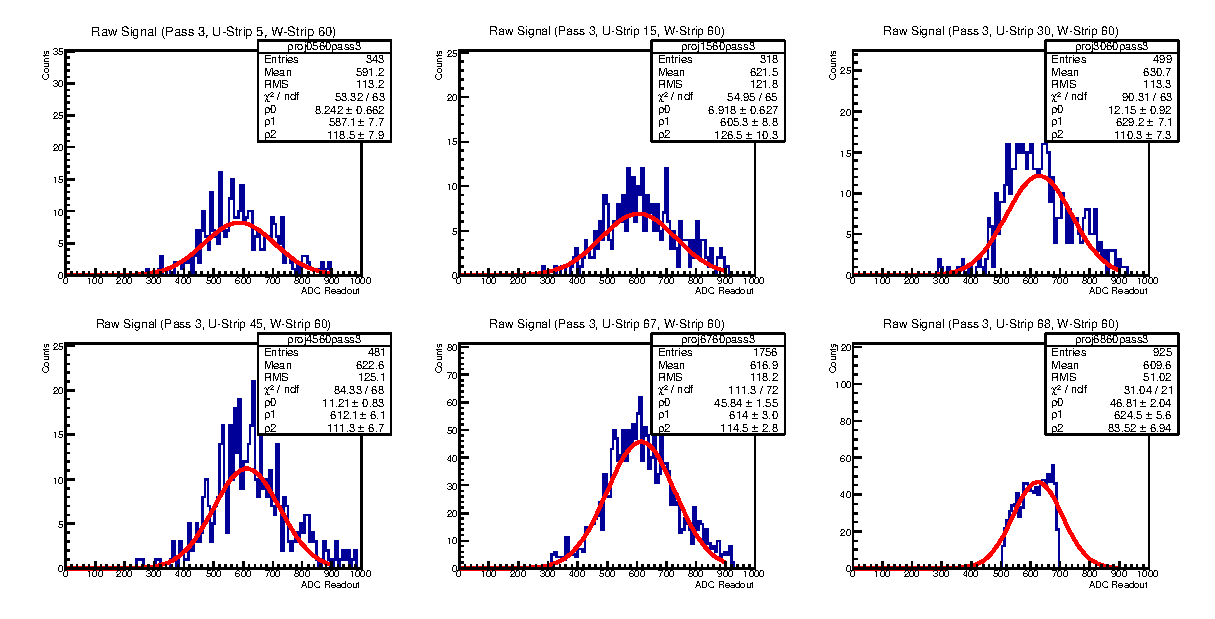
\includegraphics[height= 2.75in, keepaspectratio = true]{pass3}
    \caption{Shown is the ADC signal corresponding to signals from multiple u-strips 
    (5, 15, 30, 45, 67, and 68) and a projection of the w60 strip.}
    \label{fig:pass3}
\end{figure}

\begin{figure}[h]
    \centering
    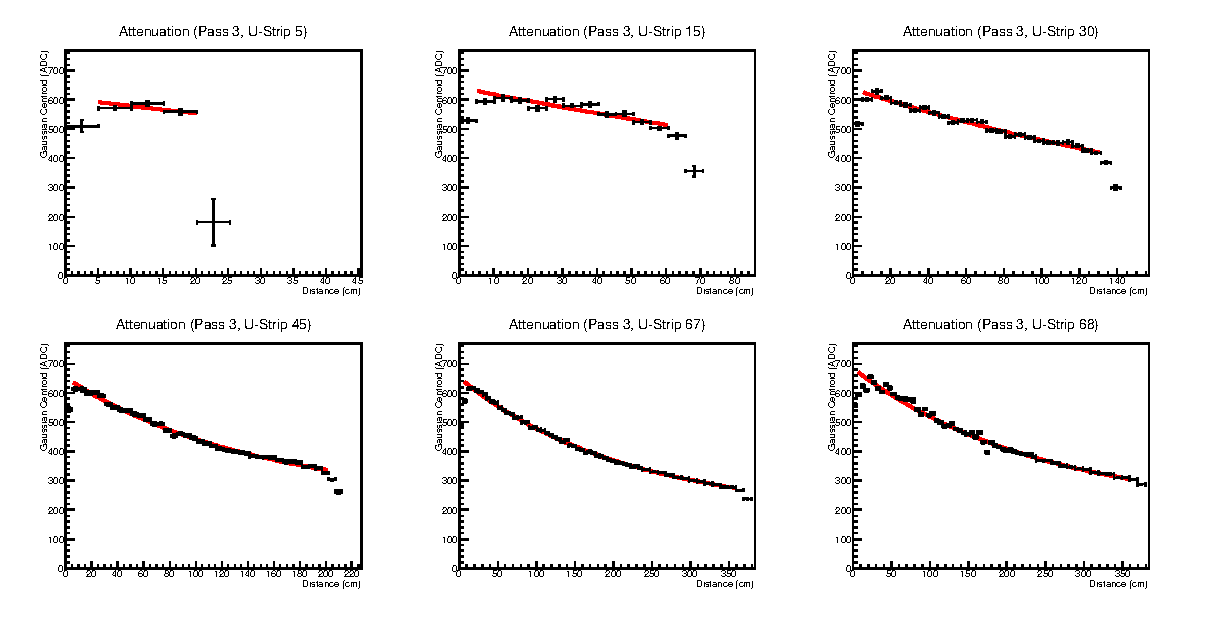
\includegraphics[height= 2.75in, keepaspectratio = true]{atpass3}
    \caption{Shown is the overall attenuation fits to the selected u-strips 
    (5, 15, 30, 45, 67, and 68).}
    \label{fig:atpass3}
\end{figure}

\clearpage
\FloatBarrier
\subsubsection{Pass 4}
\begin{itemize}
    \item Multiplicity Cut: Only events where one PMT fired for each strip were allowed.
    \item Dalitz Cut: An empircal distance sum was used to remove events that don't fall 
    into this range determined by Equation \ref{eq:totaldist}.
    \item Valid hit: Using generated events on a calculated skeleton of the pcal, each 
    pixel was determined to be valid or not.
    \item 3$\sigma$ Cut on Signal: Each signal was fit to a Gaussian in pass 2. The parameter 
    $\sigma$ from the Gaussian fit was used to cut out the events that did not lie within this function.
    \item Attenuation Corrected Intensity Cut: The ADC value measured was corrected with 
    the attenuation curves obtained from pass 2. The corrected value was summed over each 
    layer. A cut on this intensity was placed generously from 1300 to 2700
\end{itemize}


\begin{figure}[h]
    \centering
    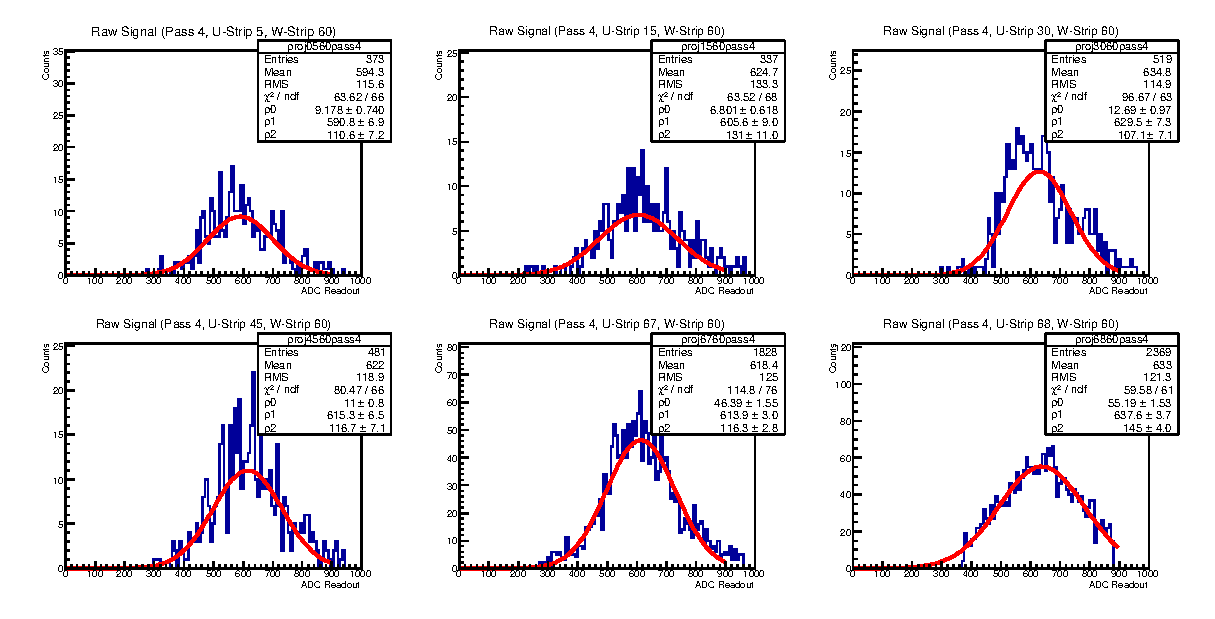
\includegraphics[height= 2.75in, keepaspectratio = true]{pass4}
    \caption{Shown is the ADC signal corresponding to signals from multiple u-strips (5, 15, 30, 45, 67, and 68) and a projection of the w60 strip.}
    \label{fig:pass4}
\end{figure}

\begin{figure}[h]
    \centering
    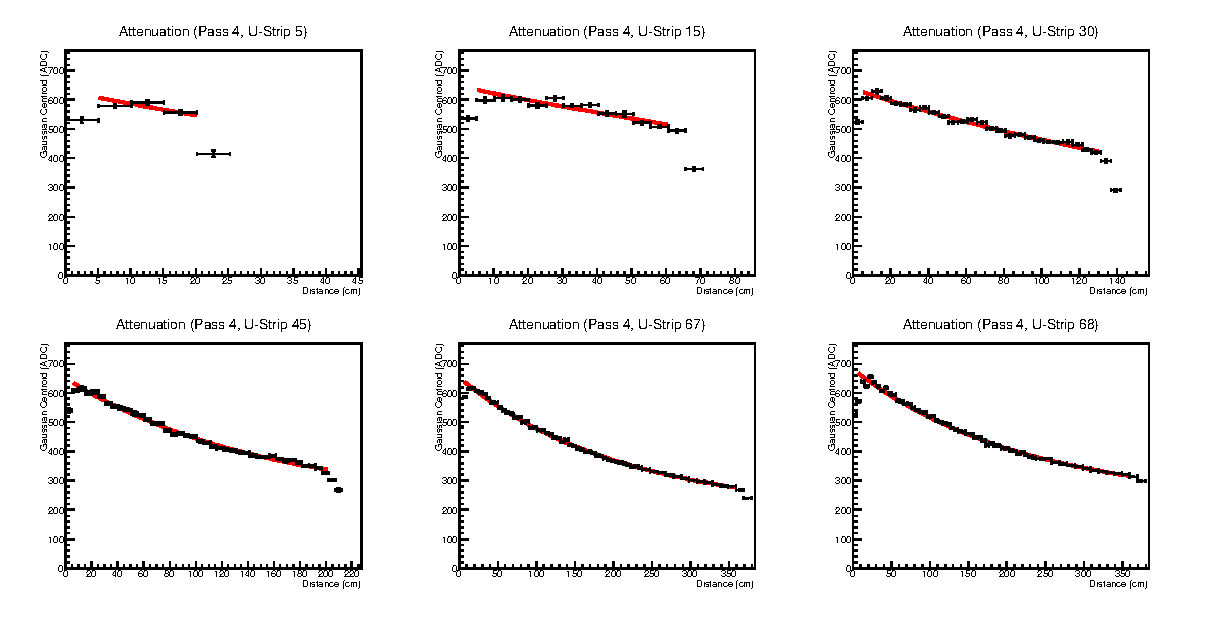
\includegraphics[height= 2.75in, keepaspectratio = true]{atpass4}
    \caption{Shown is the overall attenuation fits to the selected u-strips (5, 15, 30, 45, 67, and 68).}
    \label{fig:atpass4}
\end{figure}


\clearpage
\FloatBarrier
\subsubsection{Pass 5}
\begin{itemize}
    \item Multiplicity Cut: Only events where one PMT fired for each strip were allowed.
    \item Dalitz Cut: An empircal distance sum was used to remove events that don't fall 
    into this range determined by Equation \ref{eq:totaldist}.
    \item Valid hit: Using generated events on a calculated skeleton of the pcal, each pixel 
    was determined to be valid or not.
    \item 3$\sigma$ Cut on Signal: Each signal was fit to a Gaussian in pass 2. The parameter 
    $\sigma$ from the Gaussian fit was used to cut out the events that did not lie within this function.
    \item Attenuation Corrected Intensity Cut: The ADC value measured was corrected with the 
    attenuation curves obtained from pass 2. The corrected value was summed over each layer. 
    A cut on this intensity was placed generously from 1300 to 2700
\end{itemize}
               
               


\begin{figure}[h]
    \centering
    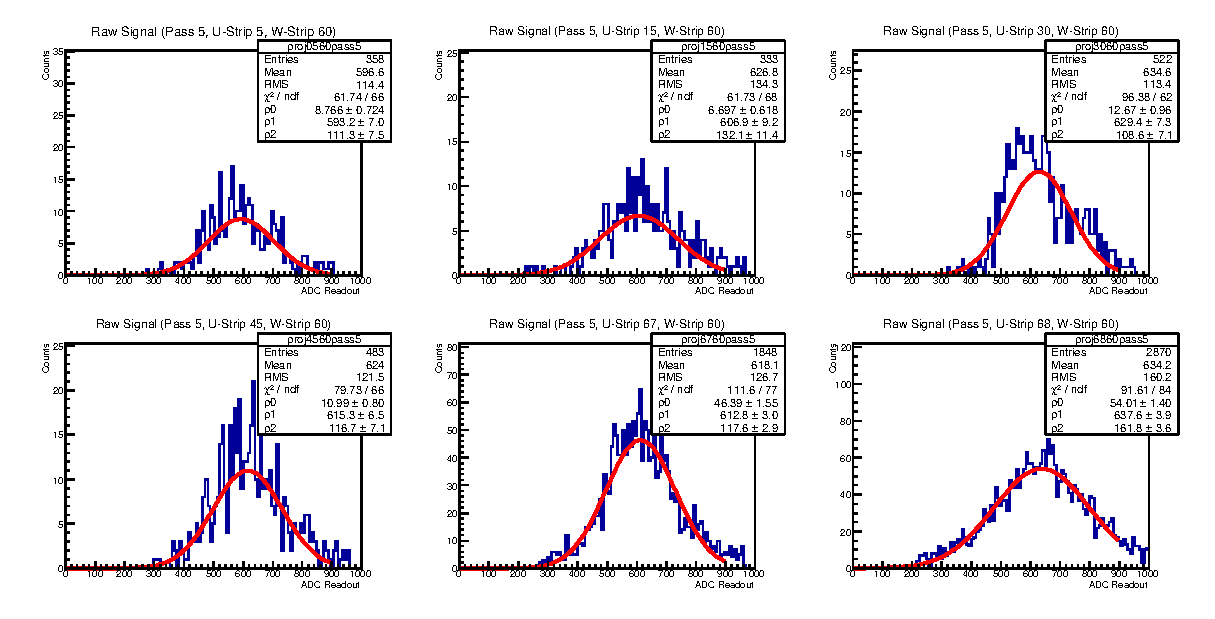
\includegraphics[height= 2.75in, keepaspectratio = true]{pass5}
    \caption{Shown is the ADC signal corresponding to signals from multiple u-strips 
    (5, 15, 30, 45, 67, and 68) and a projection of the w60 strip.}
    \label{fig:pass5}
\end{figure}

\begin{figure}[h]
    \centering
    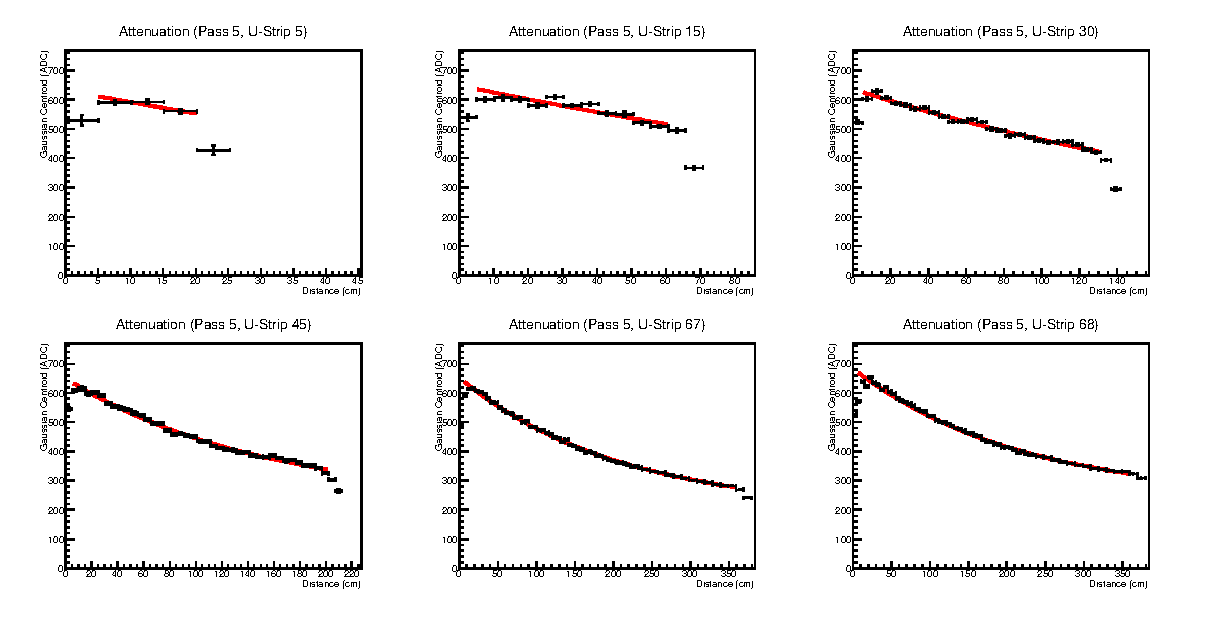
\includegraphics[height= 2.75in, keepaspectratio = true]{atpass5}
    \caption{Shown is the overall attenuation fits to the selected u-strips 
    (5, 15, 30, 45, 67, and 68).}
    \label{fig:atpass5}
\end{figure}


\FloatBarrier


\begin{figure}[h]
    \centering
    \begin{subfigure}[h]{0.3\textwidth}
        \centering
        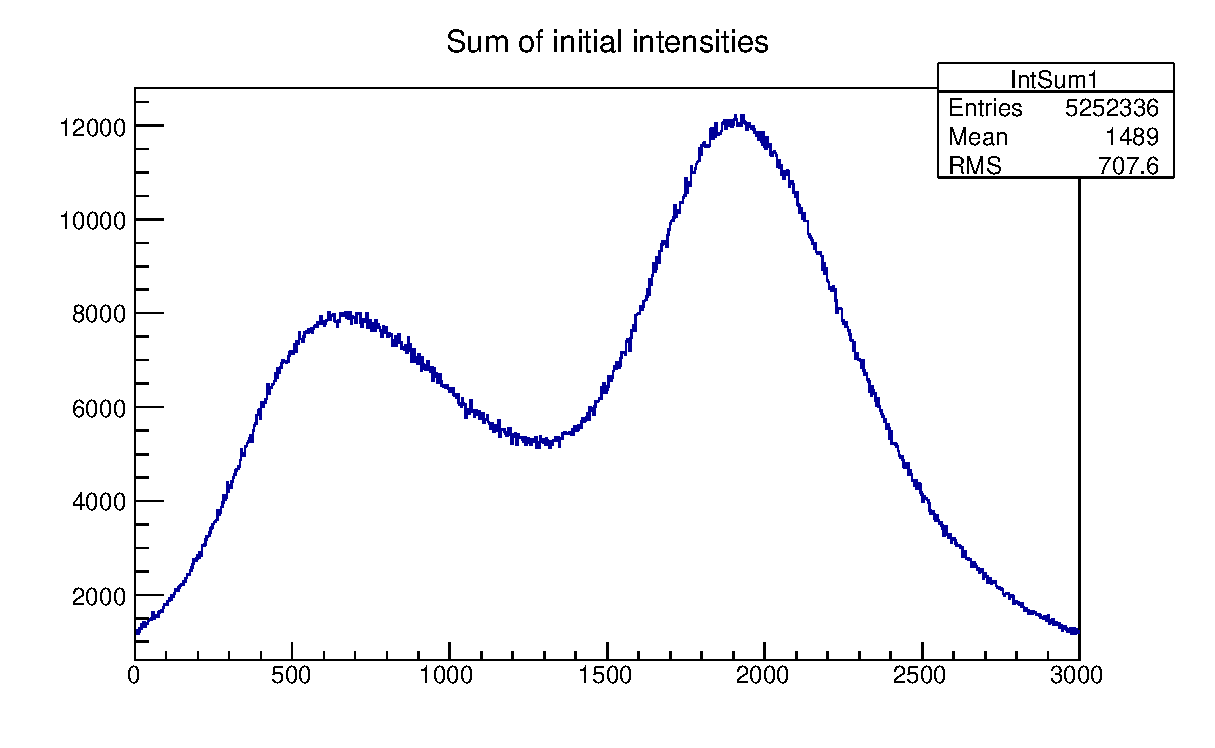
\includegraphics[width=\textwidth, keepaspectratio = true]{nocutsIsum}
        \caption{Sum of all initial intensities. No cuts.}
        \label{fig:nocutsIsum}
    \end{subfigure}
    ~
    \begin{subfigure}[h]{0.3\textwidth}
        \centering
        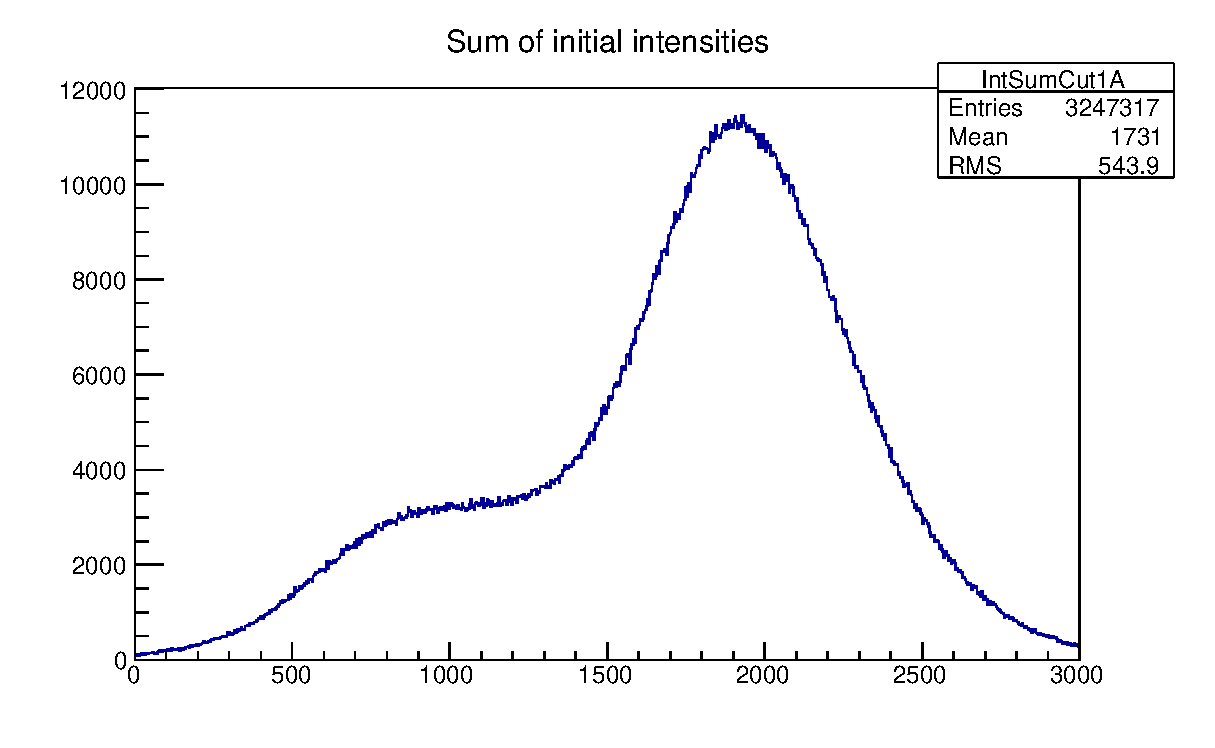
\includegraphics[width=\textwidth, keepaspectratio = true]{3sigcutIsum}
        \caption{Sum of all initial intensities. Three sigma Cut.}
        \label{fig:3sigcutIsum}
    \end{subfigure}
    ~
    \begin{subfigure}[h]{0.3\textwidth}
        \centering
        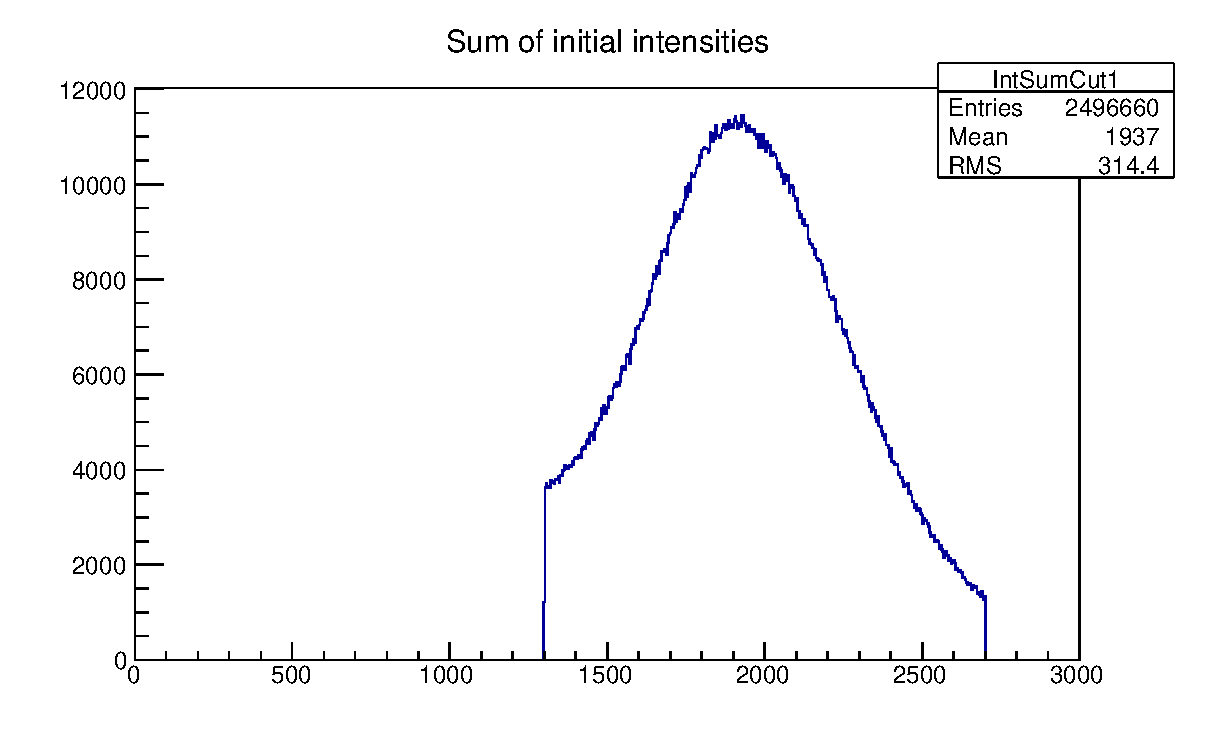
\includegraphics[width=\textwidth, keepaspectratio = true]{allcutsIsum}
        \caption{Sum of all initial intensities. Three sigma and sum Cut.}
        \label{fig:allcutsIsum}
    \end{subfigure}
    \caption{Sum of initial intensities should be near $650 \times 3 = 1950$ (after gain corrections).}
    \label{fig:intensities}
\end{figure}

\FloatBarrier
\subsection{Comparison of Fits}
Possibly the best evidence for needed cuts about each signal in an iterative process 
is seen by looking at the raw signal fits for a w strip with the possible u projections. 
These comparisons can be seen from pass 0 to pass 5 in Figures \ref{fig:w61sigfitpass0} and 
\ref{fig:w61sigfitpass5}. The difference between these signal tends to be cleaned up to a 
more Gaussian signal. By itself it is difficult to remove the backgound, but due to the correlating 
cuts on the u and v layers a reasonable output is produced.

\begin{figure}[h]
    \centering
    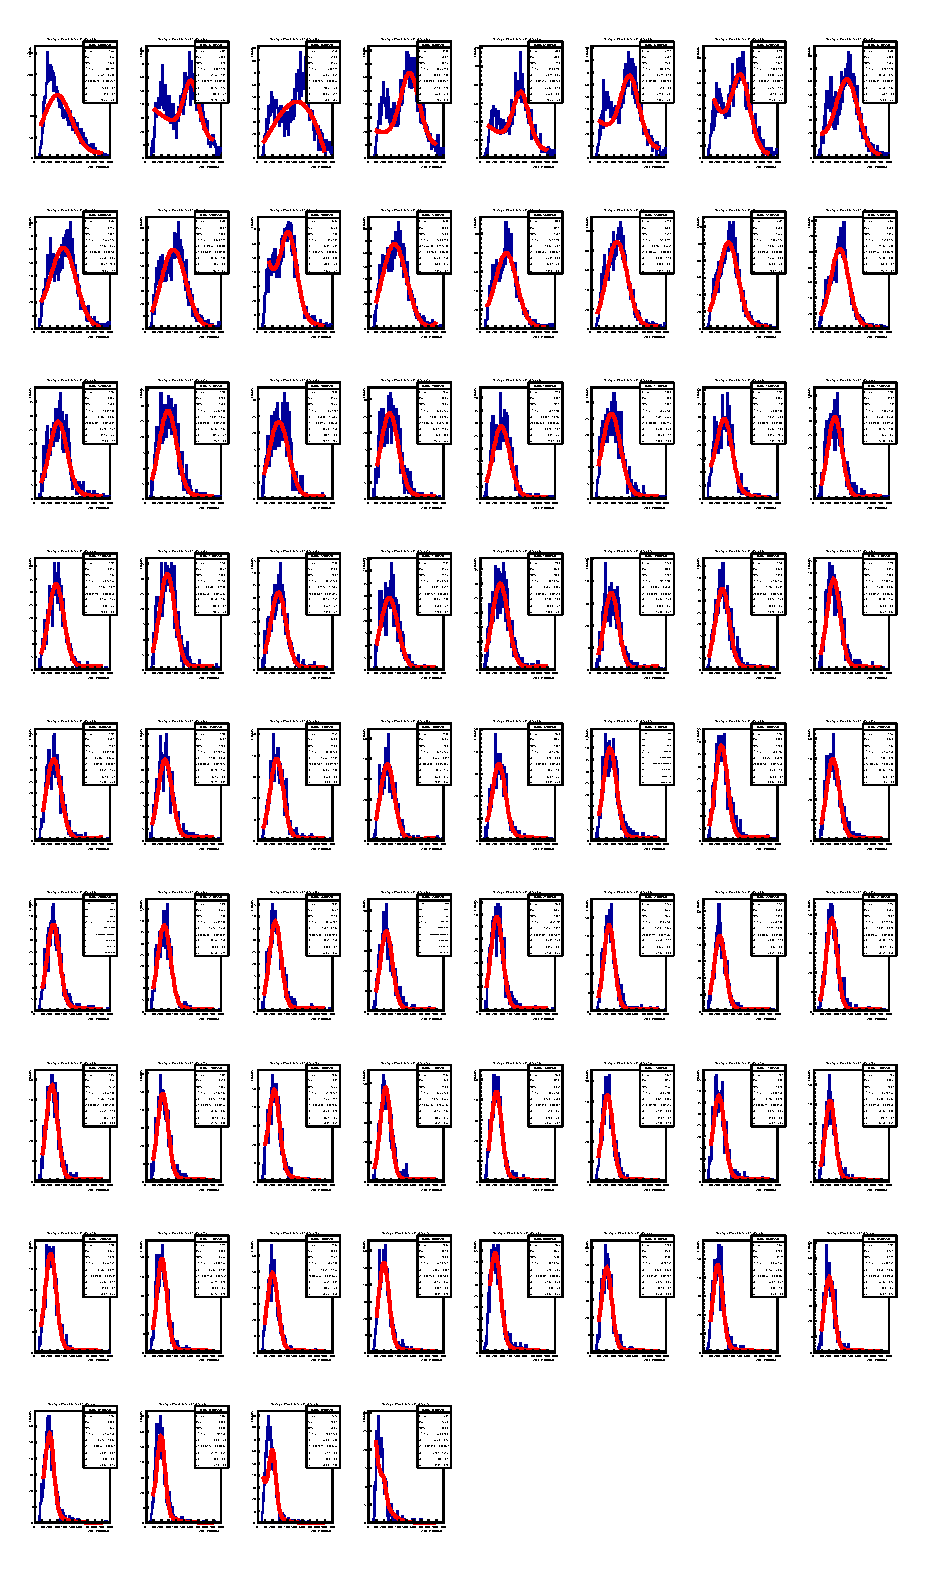
\includegraphics[width=\textwidth, height= 8in, keepaspectratio = true]{w61sigfitpass0}
    \caption{Shown is the ADC signal corresponding to signals from multiple u-strip projections of the w61 strip (pass0).}
    \label{fig:w61sigfitpass0}
\end{figure}

\begin{figure}[h]
    \centering
    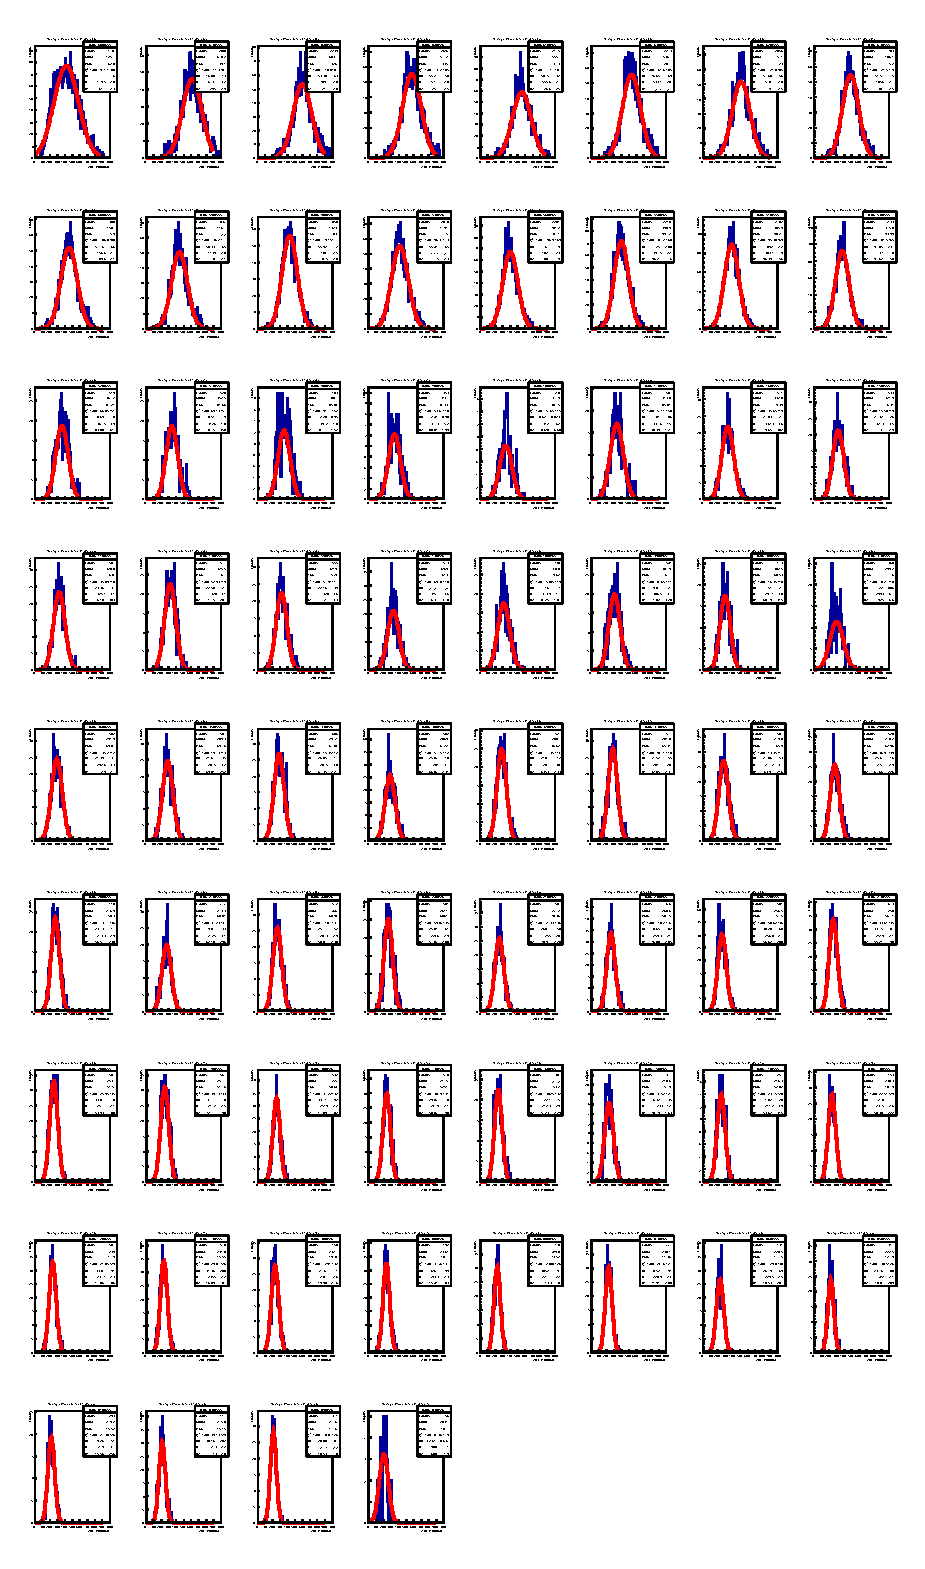
\includegraphics[width=\textwidth, height= 8in, keepaspectratio = true]{w61sigfitpass5}
    \caption{Shown is the ADC signal corresponding to signals from multiple u-strip projections of the w61 strip (pass5).}
    \label{fig:w61sigfitpass5}
\end{figure}


\FloatBarrier



\section{Light Attenuation}

Light attenuation was determined by measuring the MIP energy as a function of distance from the readout edge of each U,V,W view.  Fig.~\ref{fig:attendef} shows a schematic of how crossing strips are used to define the hit distance. The overlap of the measured strip and the crossing strip creates a trapezoidal bin formed by the overlap of two different strip orientations. The width of this physical bin is given by
\begin{equation}
    s = \frac{w}{\sin{\alpha}} = \frac{w}{\cos{\beta}}
    \label{eq:s}
\end{equation}
where $w$ is a single scintillator strip width ($\approx 4.5$cm). The strip number is converted into distance using equations \ref{eq:udist}-\ref{eq:wdist},\ref{eq:s}, plus an offset such that the distance is referenced to the center of the physical bin. 

\begin{figure}[h]
\centering
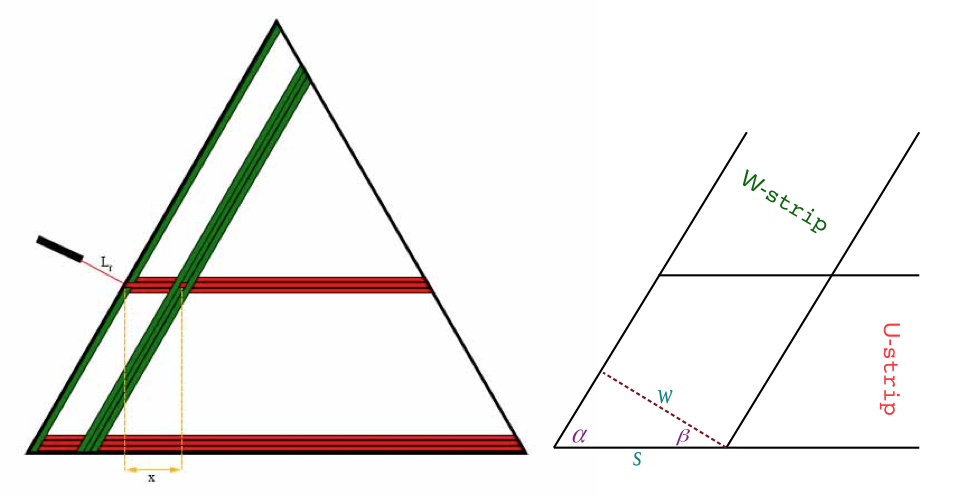
\includegraphics[height= 2in, keepaspectratio = true]{attendef}
\caption{LEFT: Schematic demonstrates the use of crossing strips to measure distance from edge of PCAL triangle. RIGHT: Outline of a generic intersection of a u and w strip. The distance between the trapezoidal
 area and the PCAL edge can be represented by a linear function of $s$.}
\label{fig:attendef}
\end{figure}

Fig.~\ref{fig:adcvdist} shows a 2-D histogram of the measured MIP energy versus the PMT number of the crossing strip.  The data clearly show the decrease in the MIP peak with distance. The next sections describe how the MIP energy for each distance slice is determined, and the fitting function used to describe the attenuation.

\begin{figure}[h]
\centering
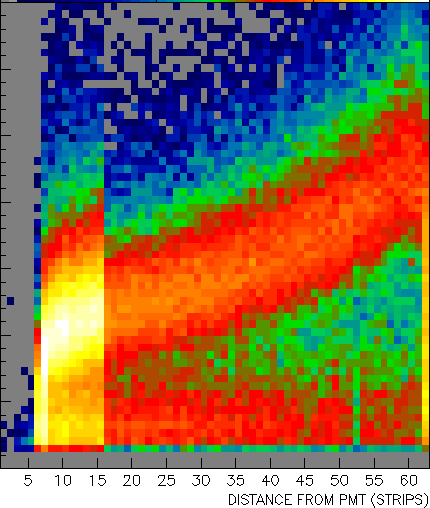
\includegraphics[width= 2.5in, keepaspectratio = true]{adcvdist}
\caption{Cosmic data showing ADC plotted vs crossing strip number.  In this case PMT 62 is closest to the readout end.}
\label{fig:adcvdist}
\end{figure}

\subsection{Fitting to MIP Peaks}
\label{Sec:fitToADCOutput}

Following event selection to isolate single pixel hits, the resulting energy loss distributions show two features:

\begin{enumerate}
\item MIP peak with a mean which is position dependent, corresponding to tracks which pass through all five scintillator layers in the measured pixel.
\item Background which diminishes with increasing pulse height and peaks near the ADC threshold.
\end{enumerate}

Fig.~\ref{fig:distribution} shows an ADC readout histogram for PMT U67, which reads out strips near the bottom edge of the PCAL.  The low energy background likely arises from tracks which partially intercept adjacent pixels but fail to exceed the threshold in those pixels.  As a result the Dalitz cut fails to exclude these tracks and incomplete collection of light occurs in the measured pixel.  The background contamination is maximum for edge strips, since there is no adjacent strip to veto 'corner clipping' muon trajectories.  The next section outlines the fitting strategy used to minimize background contributions.
	
\begin{figure}[h]
    \centering
    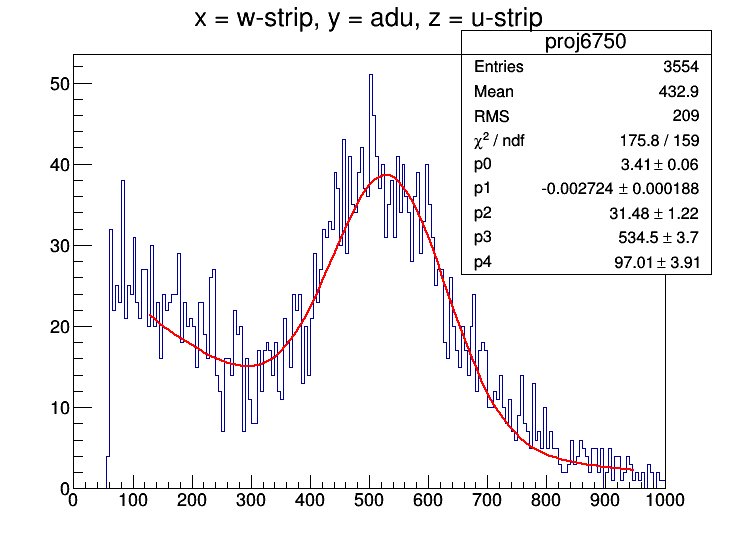
\includegraphics[width= 4in, keepaspectratio = true]{distribution}
    \caption{Example of ADC readout histogram from one U/W trapezoidal bin (U=67 W=50).  The red line is an exponential+gaussian fit.}
    \label{fig:distribution}
\end{figure}

\subsection{Fitting Strategy}

The Dalitz pixel cut works best when ADC threshold cuts can be placed close to the onset of the MIP peak in all three PMTs which view a given readout pixel.  This depends on all PMTs being well gain-matched and requires a knowledge of the light attenuation correction.  Since this is only approximately the case at the start of calibration, an iterative approach was used to progressively improve the MIP fit accuracy. 

For each iterative step, cuts to isolate the MIP peak energy are optimized using two cuts:
\begin{enumerate}
    \item Cuts on U,V,W MIP energy: A $3\sigma$ cut is placed on each MIP peak for PMTs contributing to the readout pixel based on gaussian fits.  The overall effect is to reduce the exponential background in the readout pixel. This improves the fits to some of the edges.
    \item Cuts on U+V+W MIP energy sum: The desired muon trajectory should deposit the same amount of energy into each U,V,W layer. After the initial $3\sigma$ cuts and fitting attenuation curves, individual gains can be estimated. Using the emperically found gains, a cut on the U,V,W sum of ADC signals is used to eliminate events whose partial U,V,W energies could not contribute to the sum.\end{enumerate}

\begin{figure}[h]
    \centering
    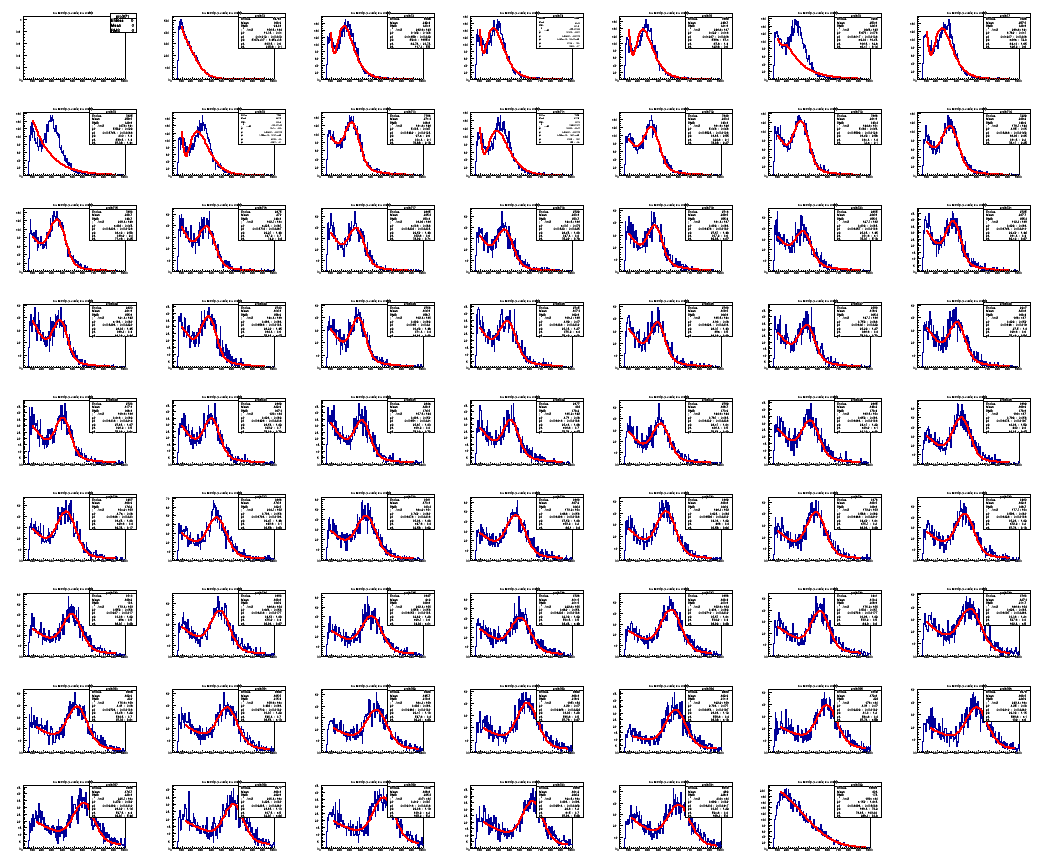
\includegraphics[width= 6in, keepaspectratio = true]{allstrip67}
    \caption{Example of all W crossing strip slices of the ADC readout from PMT U67.}
    \label{fig:allstrip67}
\end{figure}

\FloatBarrier
\subsection{Iteration Process}
For each iteration pass a $3\sigma$ cut on ADC distributions are made around the MIP peaks, determined by either the MIP signal fits or by attenuation fits.  This allows for a converging result because each cut on one U,V,W layer affects the other two. Therefore the MIP signal fits keeps improving as the attenuation fit and gains improve. 

To illustrate how the process works, the following section shows each pass of a typical iteration.  For each pass the cuts are described, followed by MIP fit plots for six representative U PMTs and a fixed crossing strip (W60).  Finally attenuation fits for each PMT are shown, which show how the multiple cuts affect each attenuation fit as a function of strip number. 

\clearpage
\FloatBarrier
\subsubsection{Pass 0}
\begin{itemize}
    \item Multiplicity Cut: Only events where one PMT fired for each strip were allowed.
    \item Dalitz Cut: An empircal distance sum was used to remove events that don't fall into 
    this range determined by Equation \ref{eq:totaldist}.
    \item Valid hit or near neighbor hit: Using generated events on a calculated skeleton of 
    the pcal, each pixel was determined to be valid or not. Extra uncertainty was allowed by 
    also marking nearest neighboring pixels.
\end{itemize}

\begin{figure}[h]
    \centering
    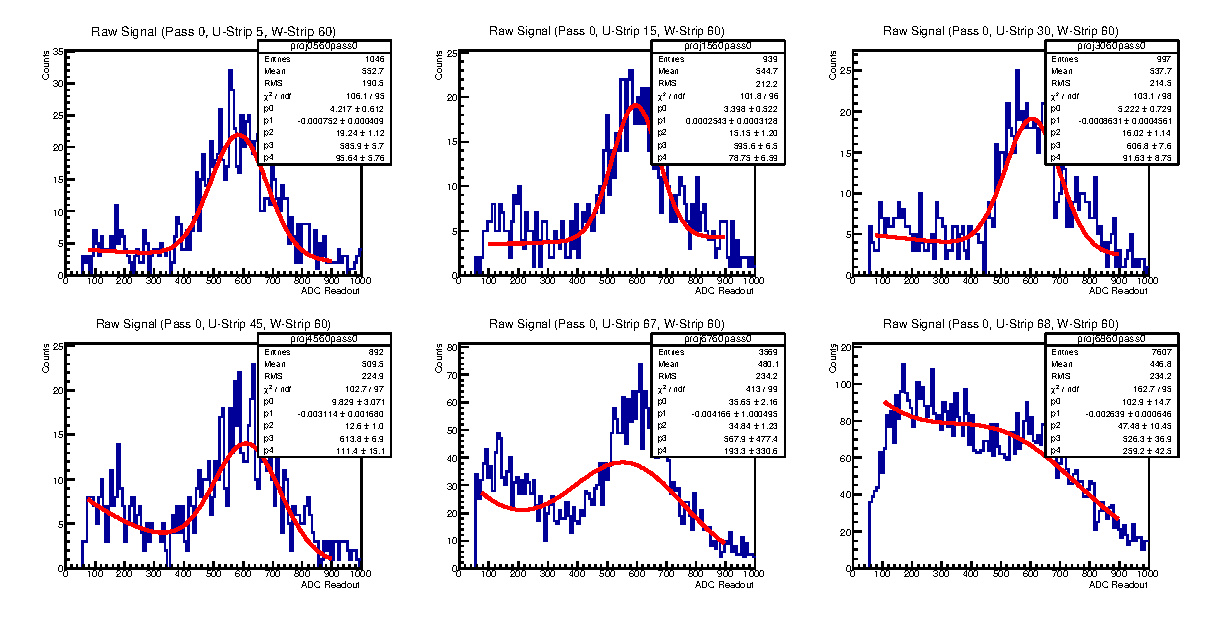
\includegraphics[height= 2.75in, keepaspectratio = true]{pass0}
    \caption{Shown is the ADC signal corresponding to signals from multiple u-strips 
    (5, 15, 30, 45, 67, and 68) and a projection of the w60 strip.}
    \label{fig:pass0}
\end{figure}

\begin{figure}[h]
    \centering
    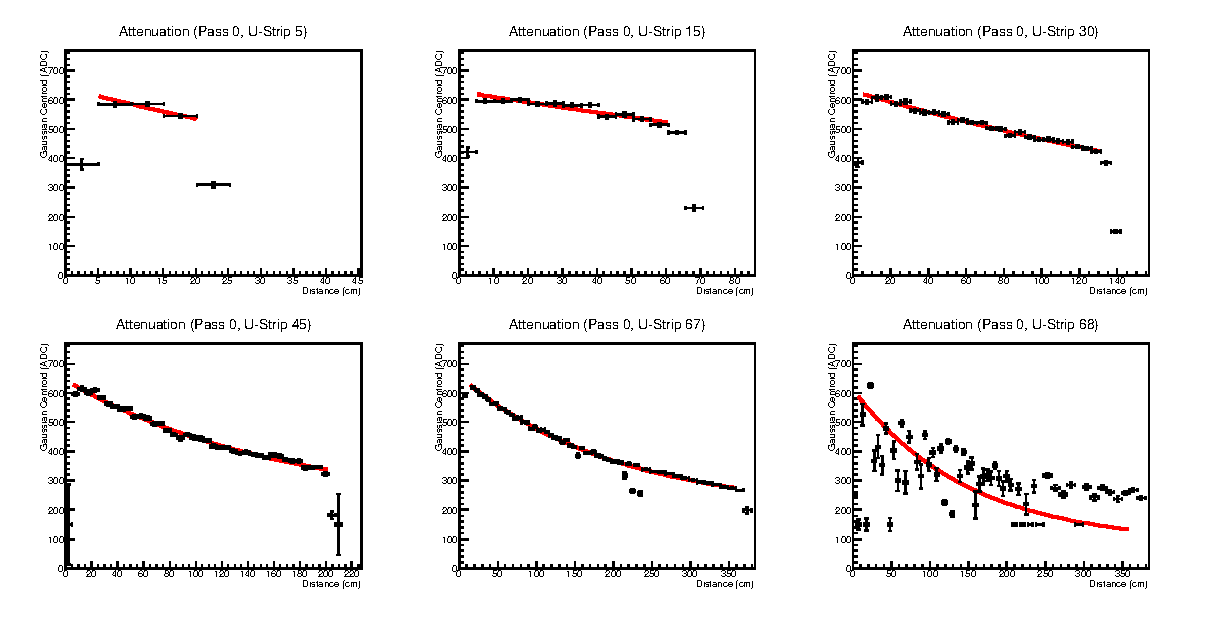
\includegraphics[height= 2.75in, keepaspectratio = true]{atpass0}
    \caption{Shown is the overall attenuation fits to the selected u-strips 
    (5, 15, 30, 45, 67, and 68).}
    \label{fig:atpass0}
\end{figure}


\clearpage
\FloatBarrier
\subsubsection{Pass 1}
\begin{itemize}
    \item Multiplicity Cut: Only events where one PMT fired for each strip were allowed.
    \item Dalitz Cut: An empircal distance sum was used to remove events that don't fall 
    into this range determined by Equation \ref{eq:totaldist}.
    \item Valid hit or near neighbor hit: Using generated events on a calculated skeleton
     of the pcal, each pixel was determined to be valid or not. Extra uncertainty was 
     allowed by also marking nearest neighboring pixels.
    \item 3$\sigma$ Cut on Signal: Each signal was fit to a Gaussian and exponential in 
    pass 0. The parameter $\sigma$ from the Gaussian fit was used to cut out the events
     that did not lie within this function.
\end{itemize}


\begin{figure}[h]
    \centering
    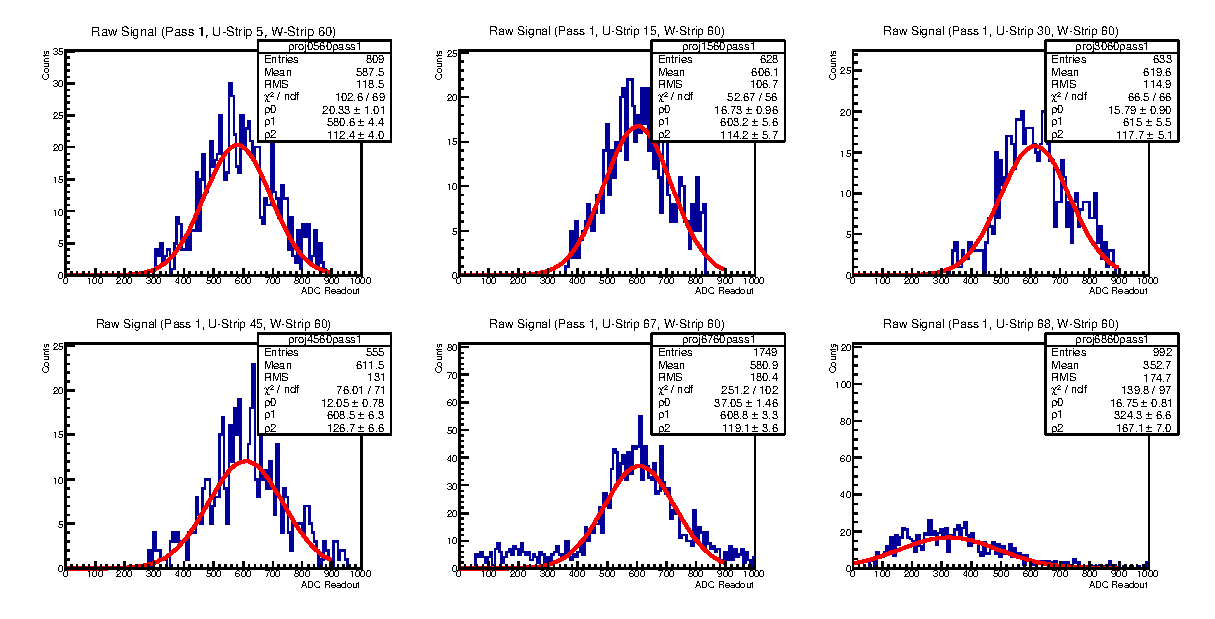
\includegraphics[height= 2.75in, keepaspectratio = true]{pass1}
    \caption{Shown is the ADC signal corresponding to signals from multiple u-strips
     (5, 15, 30, 45, 67, and 68) and a projection of the w60 strip.}
    \label{fig:pass1}
\end{figure}

\begin{figure}[h]
    \centering
    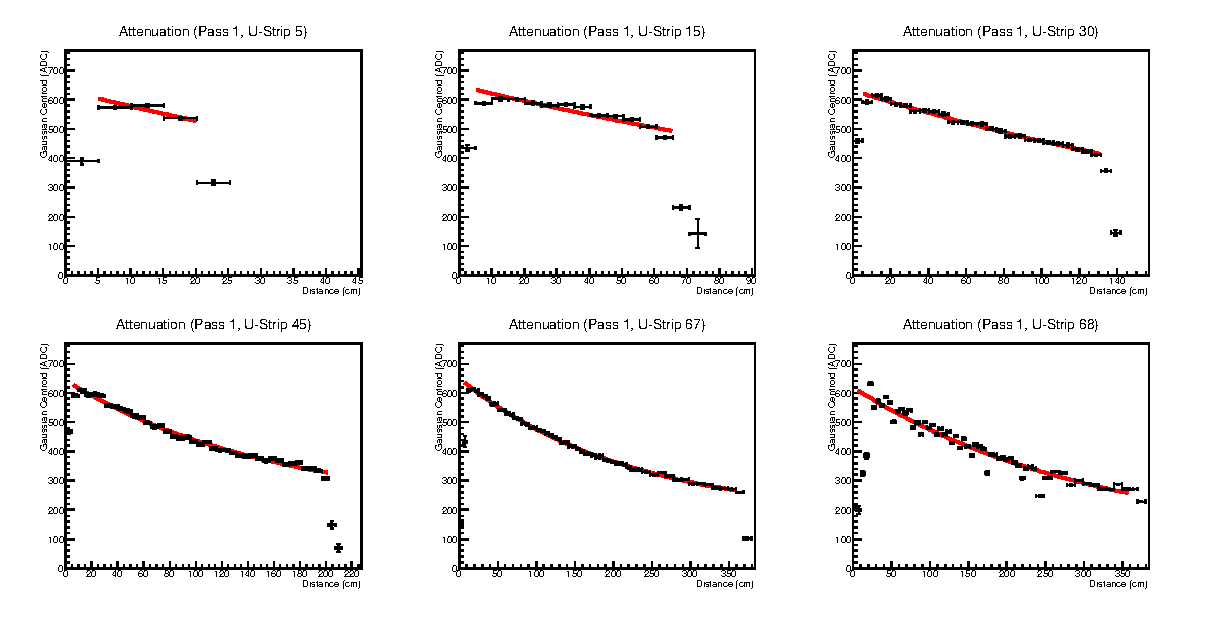
\includegraphics[height= 2.75in, keepaspectratio = true]{atpass1}
    \caption{Shown is the overall attenuation fits to the selected u-strips 
    (5, 15, 30, 45, 67, and 68).}
    \label{fig:atpass1}
\end{figure}



\clearpage
\FloatBarrier
\subsubsection{Pass 2}
\begin{itemize}
    \item Multiplicity Cut: Only events where one PMT fired for each strip were allowed.
    \item Dalitz Cut: An empircal distance sum was used to remove events that don't fall 
    into this range determined by Equation \ref{eq:totaldist}.
    \item Valid hit or near neighbor hit: Using generated events on a calculated skeleton 
    of the pcal, each pixel was determined to be valid or not. Extra uncertainty was allowed 
    by also marking nearest neighboring pixels.
    \item Cut on Attenuation Fits: When the signals where the Gaussian centroid from pass 1 
    were outside an ADC value of $\pm50$ from the attenuation fit, the obtained $\sigma$ was 
    ignored and a new cut about the attenuation fit was employed. If the centroid was close 
    to ADC value from the attenuation fit a 2$\sigma$ cut was used to remove extra background.
\end{itemize}


\begin{figure}[h]
    \centering
    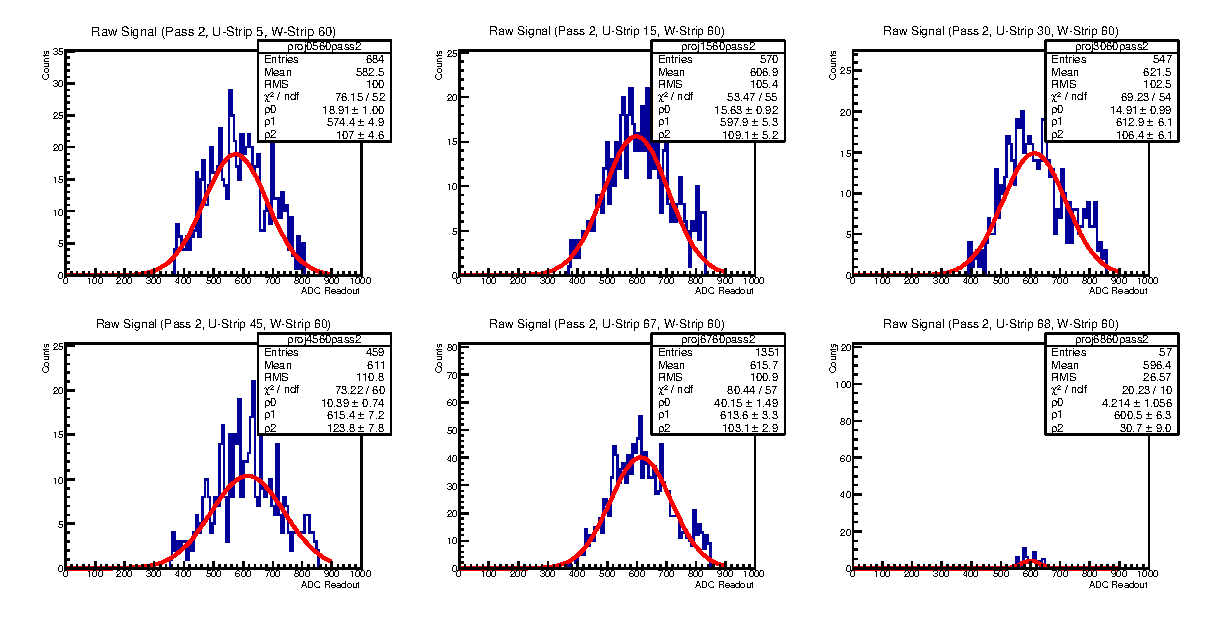
\includegraphics[height= 2.75in, keepaspectratio = true]{pass2}
    \caption{Shown is the ADC signal corresponding to signals from multiple u-strips 
    (5, 15, 30, 45, 67, and 68) and a projection of the w60 strip.}
    \label{fig:pass2}
\end{figure}

\begin{figure}[h]
    \centering
    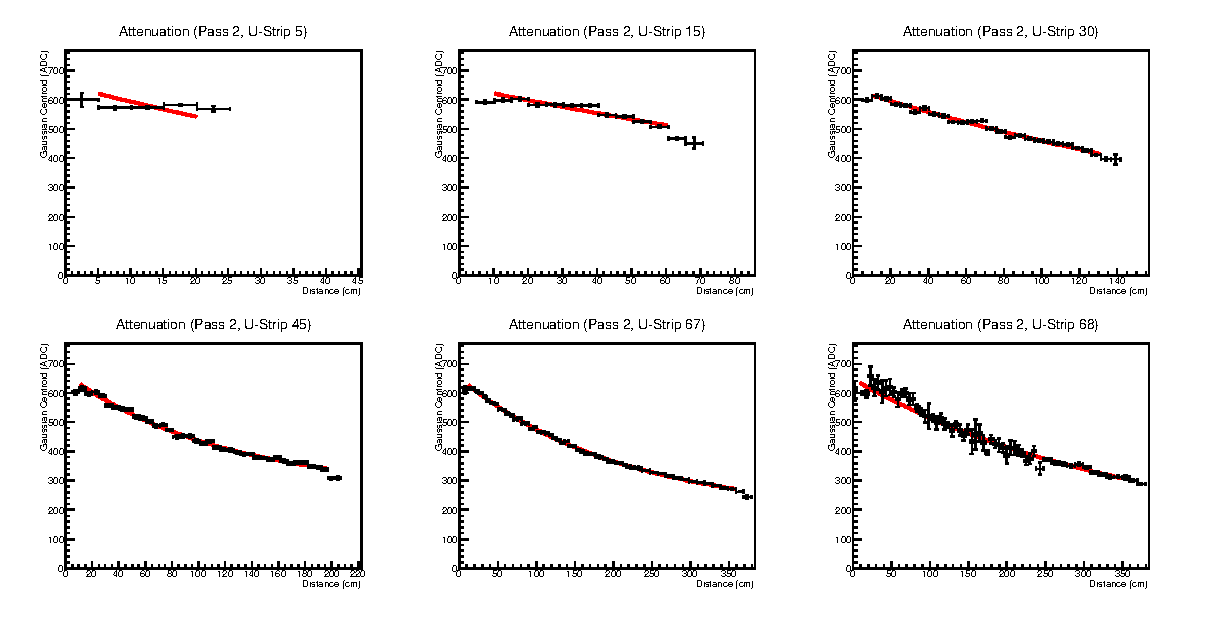
\includegraphics[height= 2.75in, keepaspectratio = true]{atpass2}
    \caption{Shown is the overall attenuation fits to the selected u-strips 
    (5, 15, 30, 45, 67, and 68).}
    \label{fig:atpass2}
\end{figure}



\clearpage
\FloatBarrier
\subsubsection{Pass 3}
\begin{itemize}
    \item Multiplicity Cut: Only events where one PMT fired for each strip were allowed.
    \item Dalitz Cut: An empircal distance sum was used to remove events that don't fall 
    into this range determined by Equation \ref{eq:totaldist}.
    \item Valid hit: Using generated events on a calculated skeleton of the pcal, each 
    pixel was determined to be valid or not.
    \item 3$\sigma$ Cut on Signal: Each signal was fit to a Gaussian in pass 2. The parameter 
    $\sigma$ from the Gaussian fit was used to cut out the events that did not lie within this function.
    \item Attenuation Corrected Intensity Cut: The ADC value measured was corrected with the 
    attenuation curves obtained from pass 2. The corrected value was summed over each layer. 
    A cut on this intensity was placed generously from 1300 to 2700
\end{itemize}

\begin{figure}[h]
    \centering
    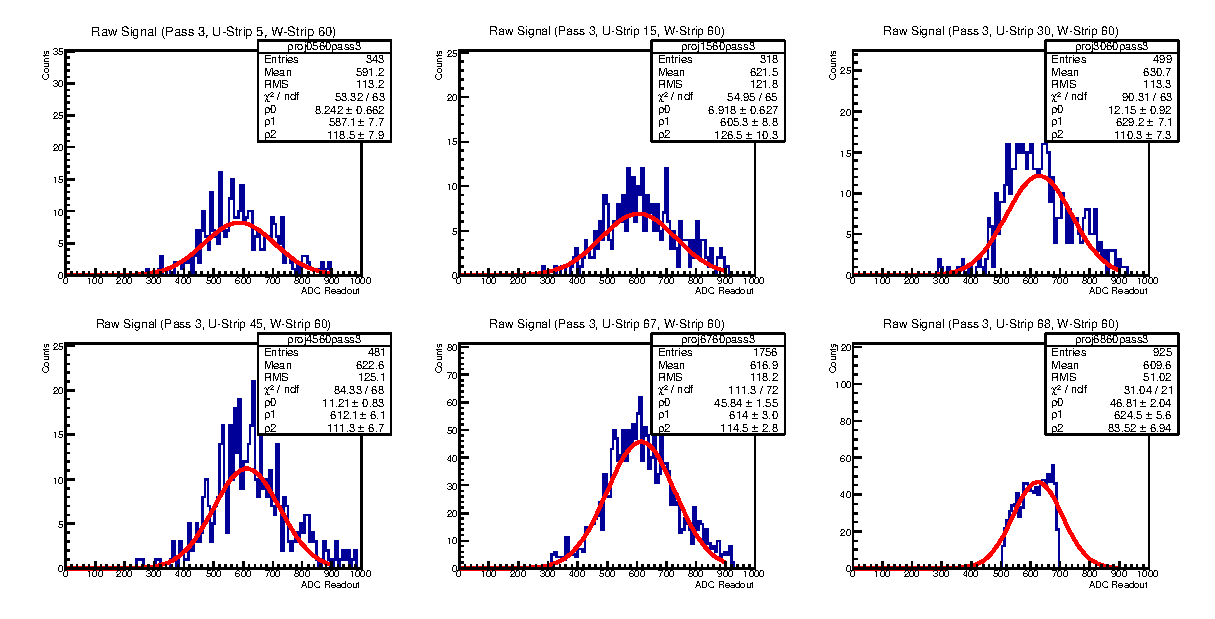
\includegraphics[height= 2.75in, keepaspectratio = true]{pass3}
    \caption{Shown is the ADC signal corresponding to signals from multiple u-strips 
    (5, 15, 30, 45, 67, and 68) and a projection of the w60 strip.}
    \label{fig:pass3}
\end{figure}

\begin{figure}[h]
    \centering
    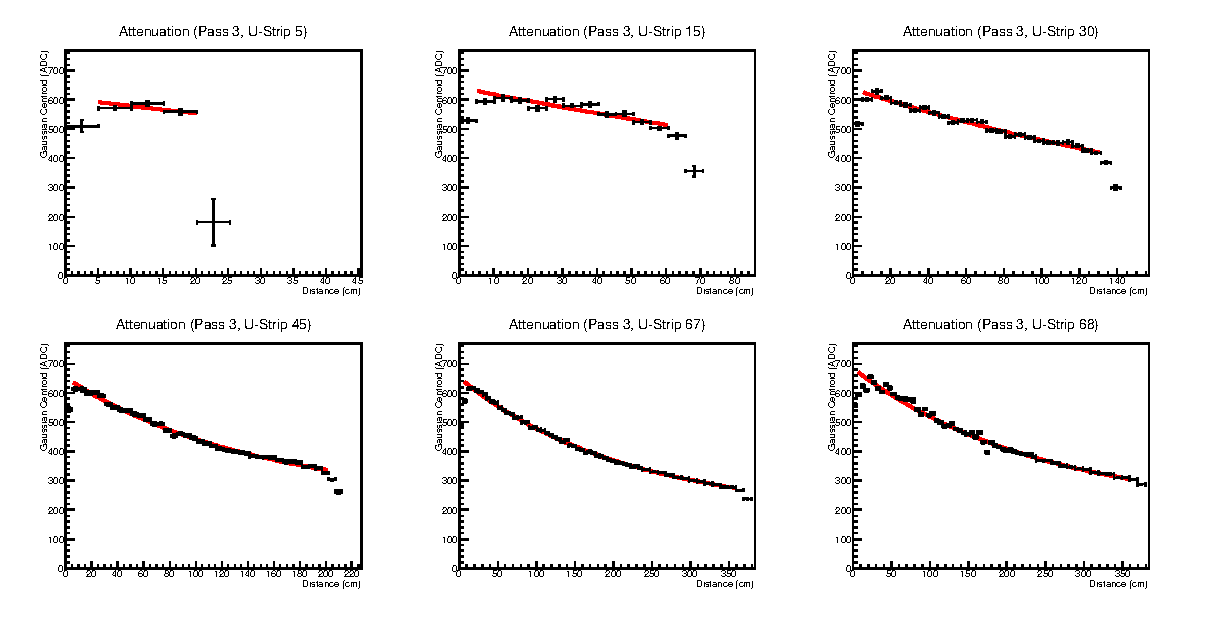
\includegraphics[height= 2.75in, keepaspectratio = true]{atpass3}
    \caption{Shown is the overall attenuation fits to the selected u-strips 
    (5, 15, 30, 45, 67, and 68).}
    \label{fig:atpass3}
\end{figure}

\clearpage
\FloatBarrier
\subsubsection{Pass 4}
\begin{itemize}
    \item Multiplicity Cut: Only events where one PMT fired for each strip were allowed.
    \item Dalitz Cut: An empircal distance sum was used to remove events that don't fall 
    into this range determined by Equation \ref{eq:totaldist}.
    \item Valid hit: Using generated events on a calculated skeleton of the pcal, each 
    pixel was determined to be valid or not.
    \item 3$\sigma$ Cut on Signal: Each signal was fit to a Gaussian in pass 2. The parameter 
    $\sigma$ from the Gaussian fit was used to cut out the events that did not lie within this function.
    \item Attenuation Corrected Intensity Cut: The ADC value measured was corrected with 
    the attenuation curves obtained from pass 2. The corrected value was summed over each 
    layer. A cut on this intensity was placed generously from 1300 to 2700
\end{itemize}


\begin{figure}[h]
    \centering
    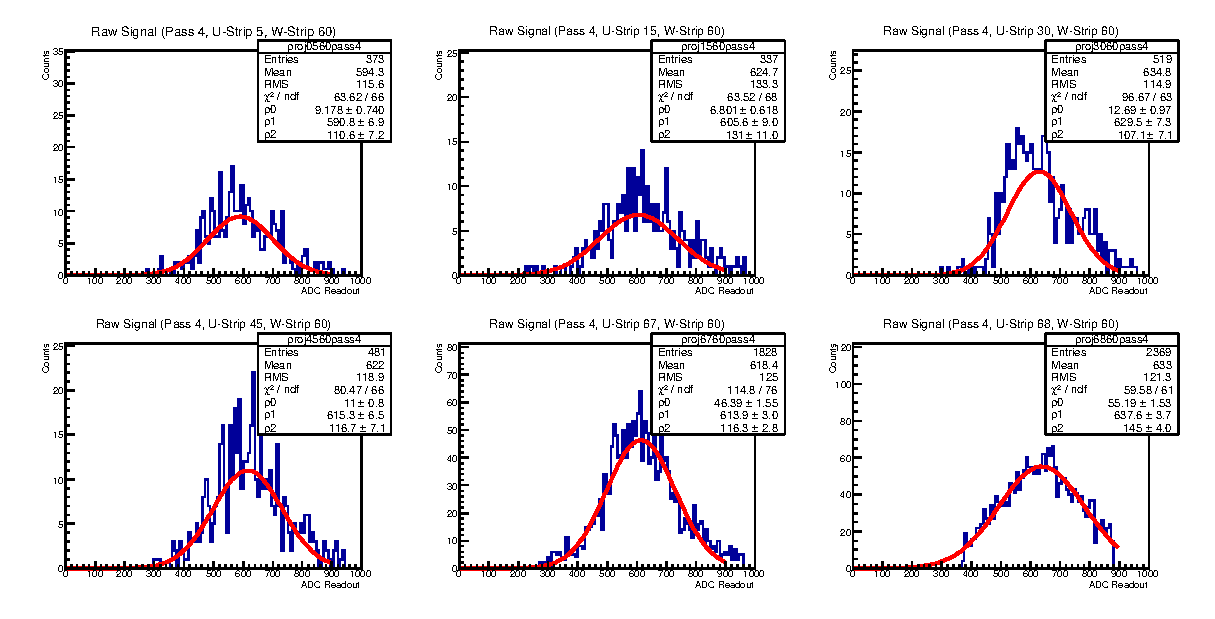
\includegraphics[height= 2.75in, keepaspectratio = true]{pass4}
    \caption{Shown is the ADC signal corresponding to signals from multiple u-strips (5, 15, 30, 45, 67, and 68) and a projection of the w60 strip.}
    \label{fig:pass4}
\end{figure}

\begin{figure}[h]
    \centering
    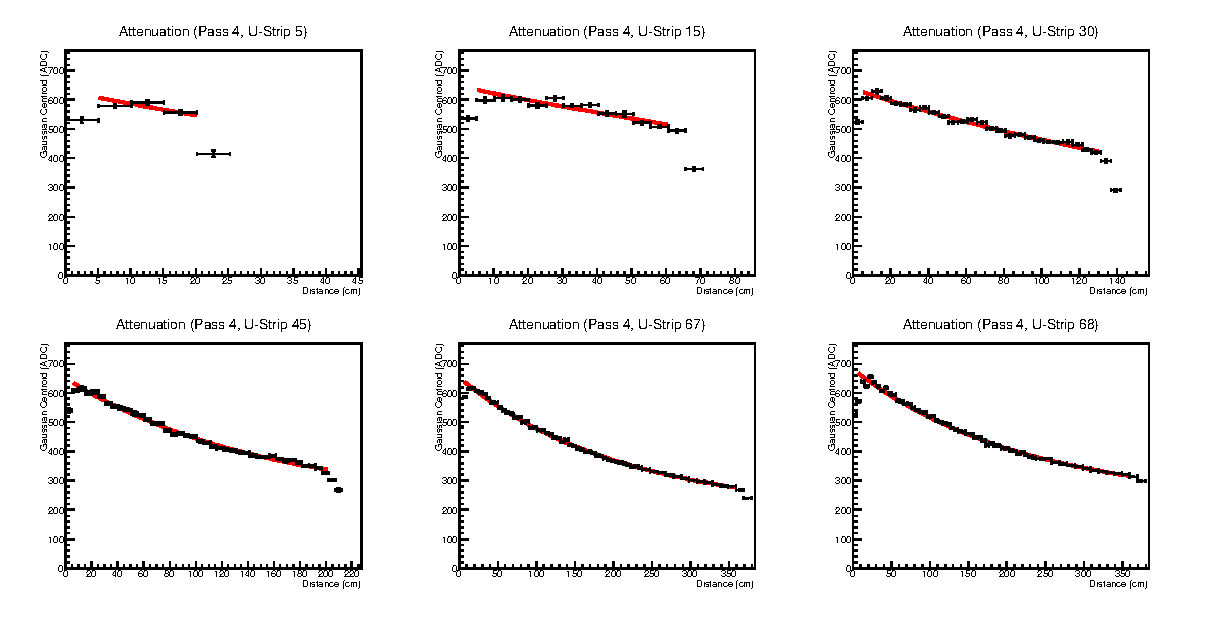
\includegraphics[height= 2.75in, keepaspectratio = true]{atpass4}
    \caption{Shown is the overall attenuation fits to the selected u-strips (5, 15, 30, 45, 67, and 68).}
    \label{fig:atpass4}
\end{figure}


\clearpage
\FloatBarrier
\subsubsection{Pass 5}
\begin{itemize}
    \item Multiplicity Cut: Only events where one PMT fired for each strip were allowed.
    \item Dalitz Cut: An empircal distance sum was used to remove events that don't fall 
    into this range determined by Equation \ref{eq:totaldist}.
    \item Valid hit: Using generated events on a calculated skeleton of the pcal, each pixel 
    was determined to be valid or not.
    \item 3$\sigma$ Cut on Signal: Each signal was fit to a Gaussian in pass 2. The parameter 
    $\sigma$ from the Gaussian fit was used to cut out the events that did not lie within this function.
    \item Attenuation Corrected Intensity Cut: The ADC value measured was corrected with the 
    attenuation curves obtained from pass 2. The corrected value was summed over each layer. 
    A cut on this intensity was placed generously from 1300 to 2700
\end{itemize}
               
               


\begin{figure}[h]
    \centering
    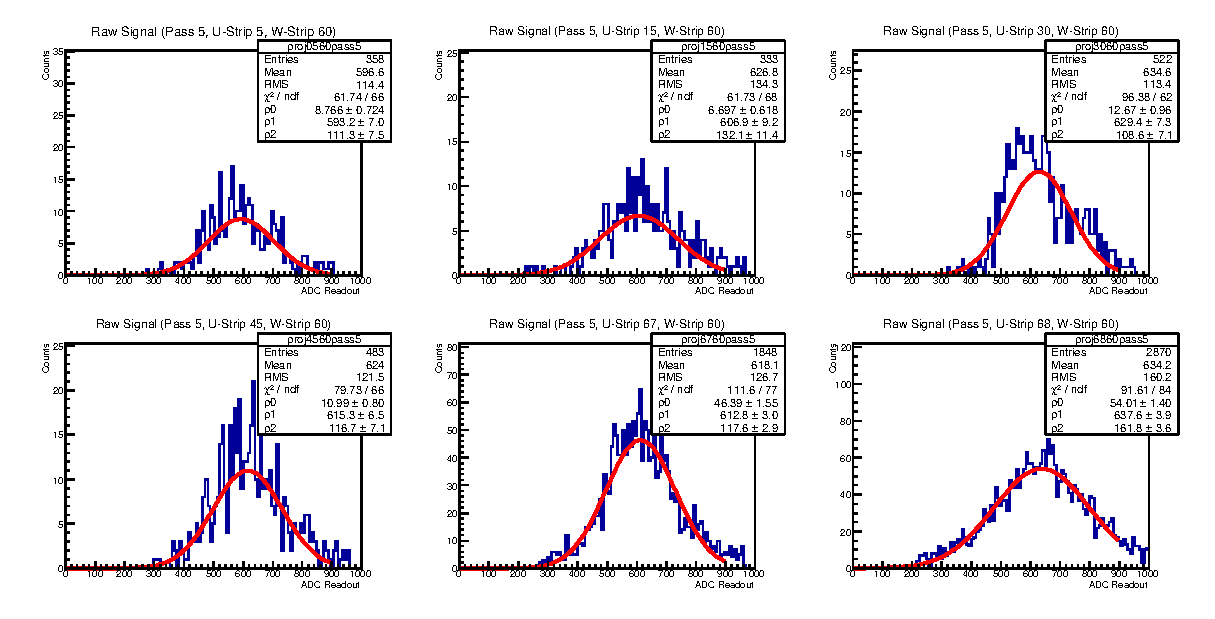
\includegraphics[height= 2.75in, keepaspectratio = true]{pass5}
    \caption{Shown is the ADC signal corresponding to signals from multiple u-strips 
    (5, 15, 30, 45, 67, and 68) and a projection of the w60 strip.}
    \label{fig:pass5}
\end{figure}

\begin{figure}[h]
    \centering
    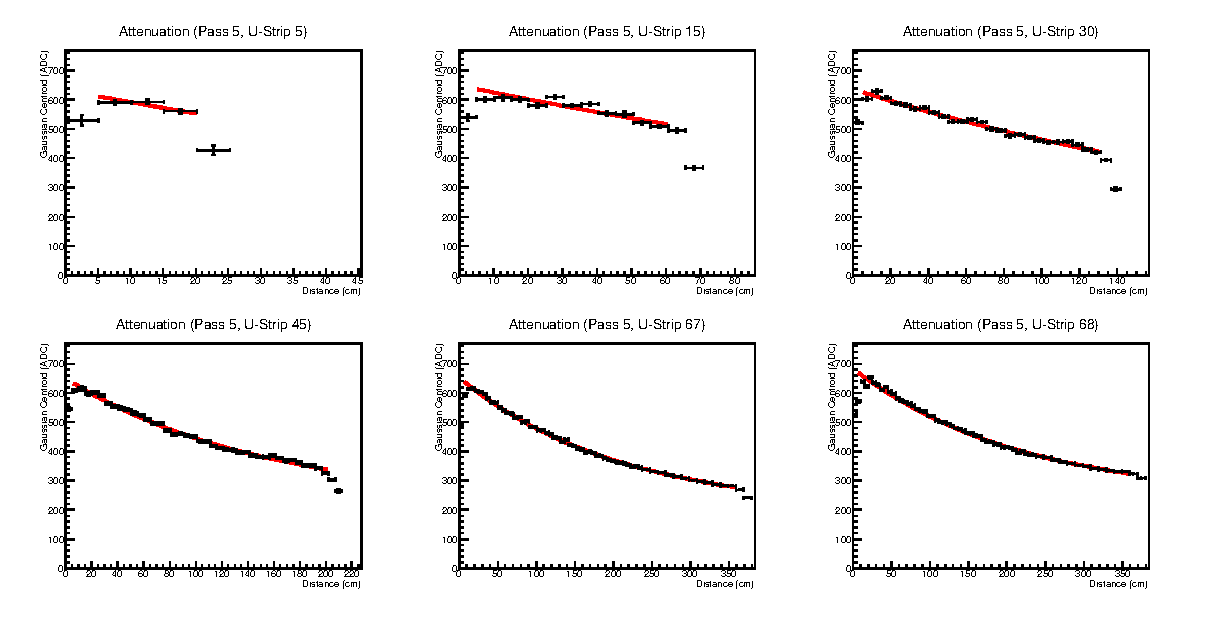
\includegraphics[height= 2.75in, keepaspectratio = true]{atpass5}
    \caption{Shown is the overall attenuation fits to the selected u-strips 
    (5, 15, 30, 45, 67, and 68).}
    \label{fig:atpass5}
\end{figure}


\FloatBarrier


\begin{figure}[h]
    \centering
    \begin{subfigure}[h]{0.3\textwidth}
        \centering
        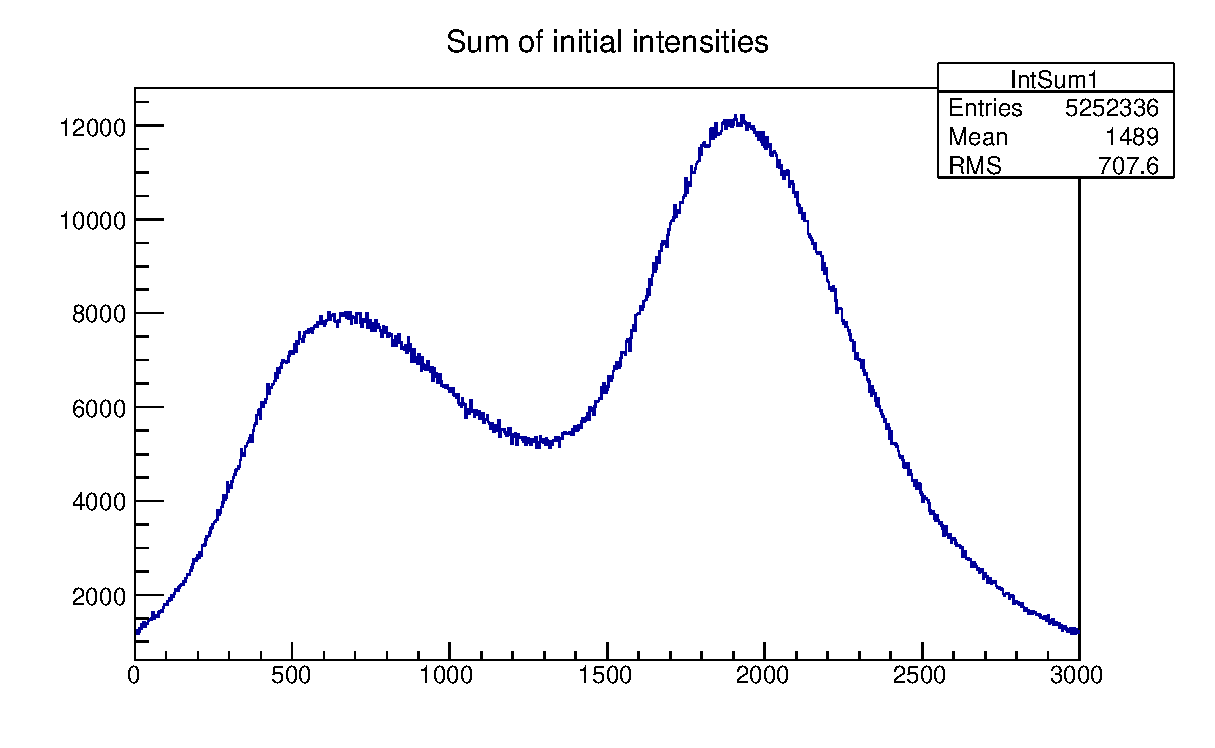
\includegraphics[width=\textwidth, keepaspectratio = true]{nocutsIsum}
        \caption{Sum of all initial intensities. No cuts.}
        \label{fig:nocutsIsum}
    \end{subfigure}
    ~
    \begin{subfigure}[h]{0.3\textwidth}
        \centering
        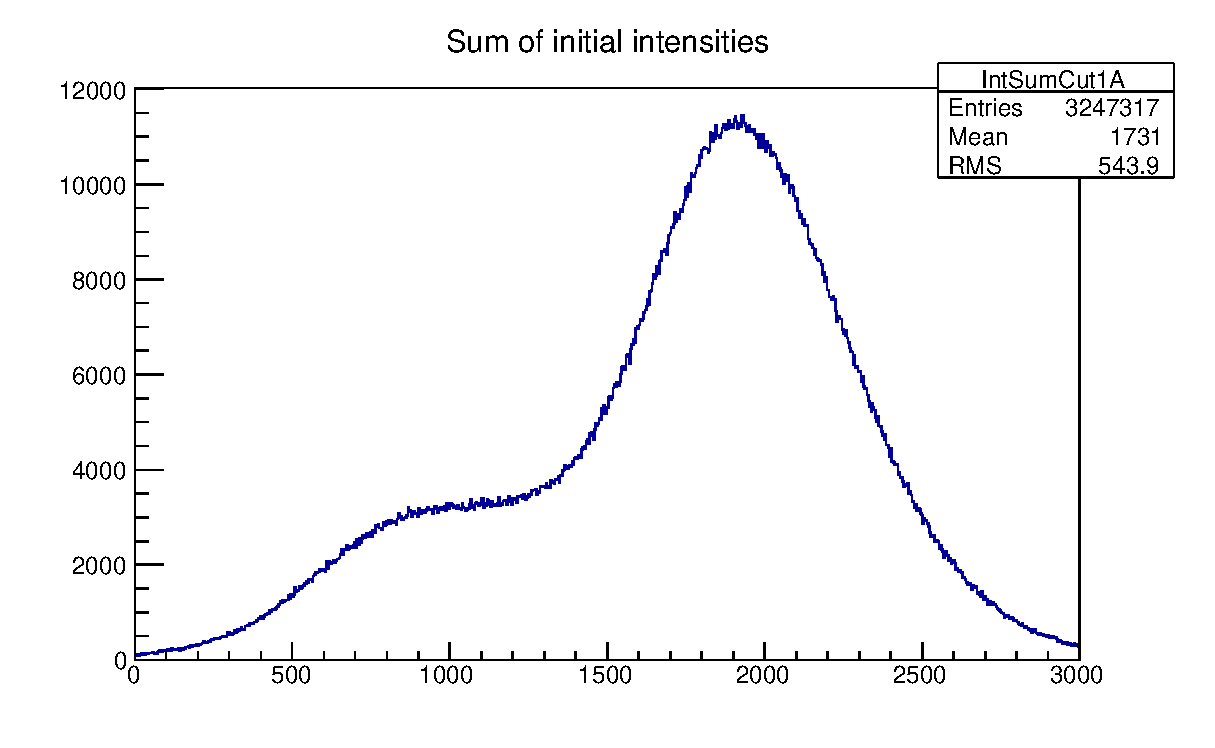
\includegraphics[width=\textwidth, keepaspectratio = true]{3sigcutIsum}
        \caption{Sum of all initial intensities. Three sigma Cut.}
        \label{fig:3sigcutIsum}
    \end{subfigure}
    ~
    \begin{subfigure}[h]{0.3\textwidth}
        \centering
        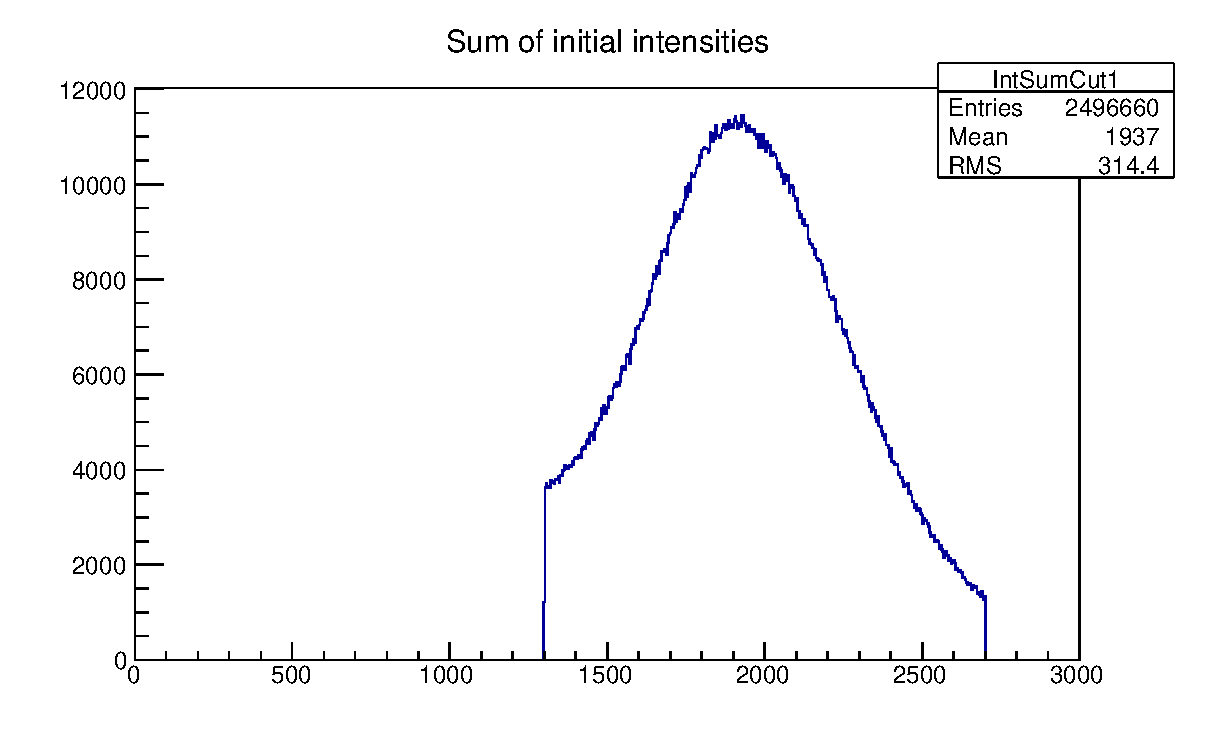
\includegraphics[width=\textwidth, keepaspectratio = true]{allcutsIsum}
        \caption{Sum of all initial intensities. Three sigma and sum Cut.}
        \label{fig:allcutsIsum}
    \end{subfigure}
    \caption{Sum of initial intensities should be near $650 \times 3 = 1950$ (after gain corrections).}
    \label{fig:intensities}
\end{figure}

\FloatBarrier
\subsection{Comparison of Fits}
Possibly the best evidence for needed cuts about each signal in an iterative process 
is seen by looking at the raw signal fits for a w strip with the possible u projections. 
These comparisons can be seen from pass 0 to pass 5 in Figures \ref{fig:w61sigfitpass0} and 
\ref{fig:w61sigfitpass5}. The difference between these signal tends to be cleaned up to a 
more Gaussian signal. By itself it is difficult to remove the backgound, but due to the correlating 
cuts on the u and v layers a reasonable output is produced.

\begin{figure}[h]
    \centering
    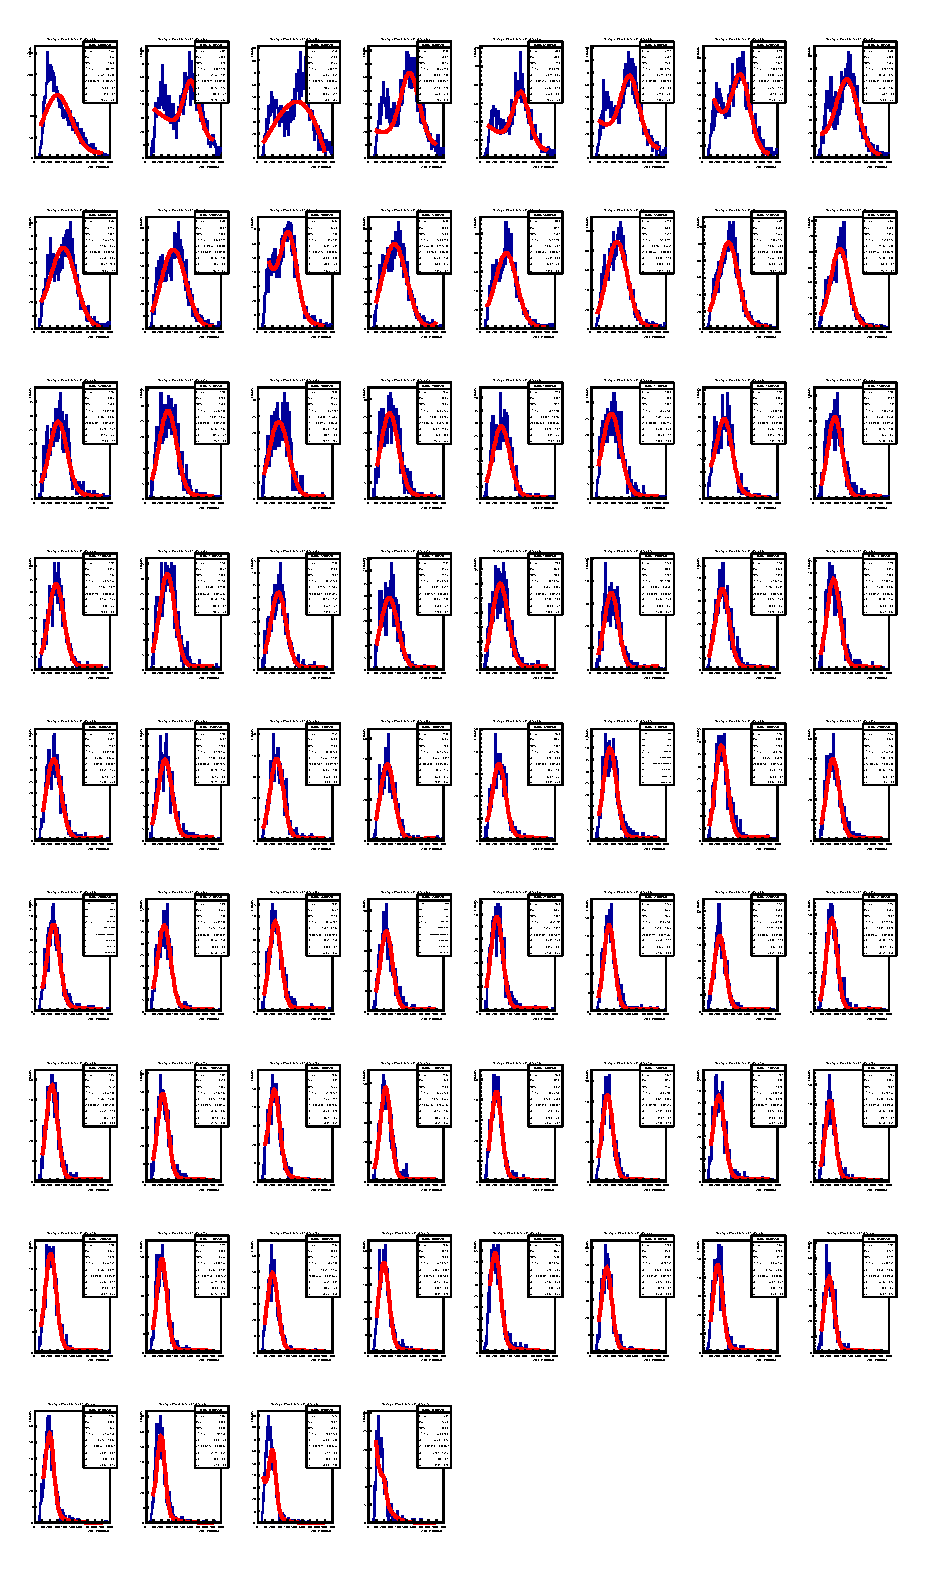
\includegraphics[width=\textwidth, height= 8in, keepaspectratio = true]{w61sigfitpass0}
    \caption{Shown is the ADC signal corresponding to signals from multiple u-strip projections of the w61 strip (pass0).}
    \label{fig:w61sigfitpass0}
\end{figure}

\begin{figure}[h]
    \centering
    \includegraphics[width=\textwidth, height= 8in, keepaspectratio = true]{w61sigfitpass5}
    \caption{Shown is the ADC signal corresponding to signals from multiple u-strip projections of the w61 strip (pass5).}
    \label{fig:w61sigfitpass5}
\end{figure}


\FloatBarrier









\FloatBarrier
\subsection{Fit Function}
\FloatBarrier
The fit function suggested in the geometry note is an  exponential (equation \ref{eq:exp}).
It is also suggested that here the distance, $L$, should include the distance from the end of the strip 
to the cosmic ray track, $L_{s}$, as well as the extra fiber length, $L_{f}$.
In other words $L = L_{s} + L_{f}$.
However to analyze the quality of fit $L_{f}$ can be treated as a constant and absorbed into the parameter 
$a$ in equation \ref{eq:exp}.

\begin{equation}
    I = e^{a + bL}
    \label{eq:exp}
\end{equation}

\begin{figure}[h]
    \centering
 %   \begin{subfigure}[h]{0.4\textwidth}
        \includegraphics[width= \textwidth, keepaspectratio = true]{exponetial67}
        \caption{Shown is a fit with equation \ref{eq:exp}, where the y axis is the ADC value and the x axis is $L_{s}$.}
        \label{fig:exponential67}
%    \end{subfigure}
    ~
%    \begin{subfigure}[h]{0.4\textwidth}
%        \includegraphics[width= \textwidth, keepaspectratio = true]{exponetialwfib67}
%        \caption{Shown is a fit with equation \ref{eq:exp}, where the y axis is the ADC value and the x axis is $L_{s} + L_{f}$.}
%        \label{fig:exponentialwfib67}
%    \end{subfigure}
%    \caption{Plotted is the fit of equation \ref{eq:exp}, where $L = L_{s}$ (a) and $L = L_{s} + L_{f}$ (b).}
%    \label{fig:expfit}
\end{figure}

As seen by figure \ref{fig:expfit}, a single exponential may not be the best fit for the data.
One might suggest a fitting function similar to equation \ref{eq:try1}, in order to separate the fiber 
attenuation from the scintillator attenuation.
However this function again can reduce to equation \ref{eq:exp} because $L_{f}$ is a constant for each 
scintillator strip and is seen not to be a good fit.


%\begin{equation}
%    \begin{split}
%        I &= a_{1}e^{b_{1}(L_{s} + L_{f})}e^{b_{2}L_{s}} \\
%          &= a_{1}e^{b_{1}(L_{s} + L_{f}) + b_{2}L_{s}} \\
%          &= a_{1}e^{(b_{1} + b_{2})L_{s} + b_{1}L_{f}} \\
%          &= a_{1}e^{b_{1}L_{f}}e^{(b_{1} + b_{2})L_{s}} \\
%          &= e^{a}e^{(b_{1} + b_{2})L_{s}} \\
%          &= e^{a}e^{bL_{s}} \\
%          &= e^{a + bL_{s}} \\
%    \end{split}
%    \label{eq:try1}
%\end{equation}

\begin{comment}
\begin{equation}
    I(L_{s})= ae^{(b_{1} + b_{2})L_{s} + b_{1}L_{f}}
    \label{eq:try1mid}
\end{equation}

\FloatBarrier
\begin{figure}[h]
    \centering
    \includegraphics[width= 3in, keepaspectratio = true]{exponential67eq9}
    \caption{Plotted is the fit of equation \ref{eq:try1mid} as a function of $L_{s}$.}
    \label{fig:try1mid}
\end{figure}
\end{comment}
\FloatBarrier


Other functional forms that could represent the data should be similar to that of an exponential.
A couple of these forms include an exponential plus a constant or a sum of exponentials.
In both cases, some considerations have to be made on the domain of the function.
The sum of two exponentials was considered to have some portion of the attenuation in the fibers to 
be different than inside the scintillator. This does not get a better fit, and does not allow any more 
information to be extracted. Therefore the function used in fitting the attenuation was chosen to be 
an exponential with an added constant as seen by Equation \ref{eq:expplusconst}.

\begin{equation}
    I(L_{s}) = ae^{bL_{s}}+c
    \label{eq:expplusconst}
\end{equation}


\FloatBarrier
\subsection{Calibration Constants}
A table of constants can be uploaded to the clas12 database once the fitting procedure is complete.
%To get the calibration constants below, parameter limits were set on equation \ref{eq:expplusconst} 
%for $200.0 < a < 900.0$, $-0.009 < b < -0.0005$, and $0.0 < c < 700.0$, based on qualitative observation on a global fit.
For strips where fewer than five points were available for fitting, either 
a single exponential or a constant term was used for the fitting function. This was done to avoid overconstraining the fit. All the fits shown are for Sector One of the PCAL.
\FloatBarrier
\vspace{5mm}

%Ufits:
\begin{figure}[h]
    \centering
    \includegraphics[width= 6.5in, height = 8in, keepaspectratio = true]{allustrips}
    \caption{Attenuation fits for U strips with U68 in the upper left hand corner. Y-axis is linear ranging from 0 to 850. X-axis varies 
    depending on the number of points in the plot.}
    \label{fig:allustrips}
\end{figure}

\FloatBarrier
%Vfits:
\begin{figure}[h]
    \centering
    \includegraphics[width= 6.5in, height = 8in, keepaspectratio = true]{allvstrips}
    \caption{Attenuation fits for V strips V62 in the upper left hand corner. Y-axis is linear ranging from 0 to 850. X-axis varies 
    depending on the number of points in the plot.}
    \label{fig:allvstrips}
\end{figure}


\FloatBarrier

%Wfits:
\begin{figure}[h]
    \centering
    \includegraphics[width= 6.5in, height = 8in, keepaspectratio = true]{allwstrips}
    \caption{Attenuation fits for V strips V62 in the upper left hand corner. Y-axis is linear ranging from 0 to 850. X-axis varies 
    depending on the number of points in the plot.}
    \label{fig:allustrips}
\end{figure}

\FloatBarrier
\begin{table}[h]
        \centering{}
        \scalebox{0.75}{
        \begin{tabular}{|c|c|c|c|}
            \hline
            U-Strip &  Parameter $a$  &Parameter $b$  & Parameter $c$ \\ \hline
1   &   650   &   0   &   0  \\  \hline  
2   &   650   &   0   &   0  \\  \hline  
3   &   650   &   -0.009   &   0  \\  \hline  
4   &   650   &   -0.009   &   0  \\  \hline  
5   &   616.113   &   -0.00639717   &   33.8858  \\  \hline  
6   &   649.996   &   -0.00717551   &   0.0046356  \\  \hline  
7   &   649.968   &   -0.00318808   &   0.0319326  \\  \hline  
8   &   649.972   &   -0.00232476   &   0.0273016  \\  \hline  
9   &   649.146   &   -0.00112904   &   0.854413  \\  \hline  
10   &   649.999   &   -0.00281005   &   0.000286188  \\  \hline  
11   &   649.993   &   -0.00286292   &   0.00718601  \\  \hline  
12   &   650   &   -0.0041656   &   0.000445736  \\  \hline  
13   &   650   &   -0.003283   &   0.000103724  \\  \hline  
14   &   649.997   &   -0.00376077   &   5.37227e-06  \\  \hline  
15   &   650.001   &   -0.00339912   &   6.96689e-06  \\  \hline  
16   &   649.997   &   -0.00305411   &   8.14649e-06  \\  \hline  
17   &   649.999   &   -0.00345134   &   9.95183e-09  \\  \hline  
18   &   649.998   &   -0.00310718   &   4.19396e-07  \\  \hline  
19   &   650   &   -0.00311517   &   5.01049e-06  \\  \hline  
20   &   650   &   -0.00281725   &   6.09084e-06  \\  \hline  
21   &   650   &   -0.00315783   &   3.38135e-05  \\  \hline  
22   &   650   &   -0.00328681   &   2.55834e-08  \\  \hline  
23   &   650   &   -0.00316776   &   2.15877e-05  \\  \hline  
24   &   649.999   &   -0.00317021   &   4.66803e-05  \\  \hline  
25   &   650   &   -0.00327065   &   5.9556e-06  \\  \hline  
26   &   650.001   &   -0.00309179   &   1.40689e-08  \\  \hline  
27   &   551.087   &   -0.00385902   &   98.9141  \\  \hline  
28   &   649.997   &   -0.00307714   &   7.49416e-05  \\  \hline  
29   &   419.522   &   -0.00552754   &   230.477  \\  \hline  
30   &   650   &   -0.00316014   &   0.000130702  \\  \hline  
31   &   650.001   &   -0.00312815   &   2.25921e-06  \\  \hline  
32   &   585.658   &   -0.00373922   &   64.3455  \\  \hline  
33   &   581.001   &   -0.00374214   &   68.997  \\  \hline  
34   &   650.002   &   -0.00328878   &   0.000131253  \\  \hline  
35   &   650   &   -0.00332314   &   1.43305e-05  \\  \hline  
36   &   649.998   &   -0.00340294   &   1.07435e-07  \\  \hline  
37   &   556.399   &   -0.00428136   &   93.5991  \\  \hline  
38   &   483.854   &   -0.00534903   &   166.146  \\  \hline  
39   &   482.458   &   -0.00431684   &   167.541  \\  \hline  
40   &   392.765   &   -0.00669036   &   257.235  \\  \hline  
41   &   499.22   &   -0.00443664   &   150.78  \\  \hline  
42   &   513.839   &   -0.00445738   &   136.164  \\  \hline  
43   &   581.507   &   -0.00388427   &   68.4914  \\  \hline  
44   &   391.463   &   -0.00757633   &   258.536  \\  \hline  
45   &   434.393   &   -0.00632194   &   215.608  \\  \hline  
46   &   463.813   &   -0.00513914   &   186.187  \\  \hline  
47   &   413.809   &   -0.00605594   &   236.189  \\  \hline  
48   &   442.234   &   -0.00592955   &   207.766  \\  \hline  
49   &   509.976   &   -0.00449146   &   140.024  \\  \hline  
50   &   443.895   &   -0.00614484   &   206.105  \\  \hline  
51   &   425.765   &   -0.00641114   &   224.233  \\  \hline  
52   &   504.812   &   -0.00511618   &   145.188  \\  \hline  
53   &   454.838   &   -0.0061679   &   195.162  \\  \hline  
54   &   406.411   &   -0.00766326   &   243.589  \\  \hline  
55   &   415.976   &   -0.00690821   &   234.026  \\  \hline  
56   &   421.326   &   -0.00710769   &   228.675  \\  \hline  
57   &   435.635   &   -0.00660386   &   214.362  \\  \hline  
58   &   411.518   &   -0.00663318   &   238.483  \\  \hline  
59   &   438.882   &   -0.00625669   &   211.118  \\  \hline  
60   &   423.763   &   -0.00618908   &   226.238  \\  \hline  
61   &   444.671   &   -0.0063621   &   205.328  \\  \hline  
62   &   438.481   &   -0.00674885   &   211.519  \\  \hline  
63   &   437.138   &   -0.00564978   &   212.862  \\  \hline  
64   &   482.525   &   -0.00495599   &   167.473  \\  \hline  
65   &   473.388   &   -0.00516614   &   176.613  \\  \hline  
66   &   465.633   &   -0.00500512   &   184.367  \\  \hline  
67   &   455.941   &   -0.00479029   &   194.059  \\  \hline  
68   &   410.201   &   -0.00506009   &   239.798  \\  \hline  
        \end{tabular}
        }
        \caption{Calibration Constants for the U layer.}
        \label{tab:UattenC}
\end{table}


\begin{table}[h]
        \centering
        \scalebox{0.75}{
        \begin{tabular}{|c|c|c|c|}
            \hline
            V-Strip &  Parameter $a$  &Parameter $b$  & Parameter $c$ \\ \hline
1   &   650.002   &   0   &   0  \\  \hline  
2   &   649.999   &   0   &   0  \\  \hline  
3   &   650.001   &   -0.009   &   0  \\  \hline  
4   &   650.001   &   -0.009   &   8.41036e-07  \\  \hline  
5   &   650   &   -0.00794645   &   5.04738e-06  \\  \hline  
6   &   649.225   &   -0.00402729   &   0.773706  \\  \hline  
7   &   341.165   &   -0.009   &   308.835  \\  \hline  
8   &   649.999   &   -0.0043402   &   0.000921065  \\  \hline  
9   &   650   &   -0.00346629   &   0.00030414  \\  \hline  
10   &   409.661   &   -0.0073313   &   240.338  \\  \hline  
11   &   650   &   -0.0036951   &   0.000157707  \\  \hline  
12   &   543.255   &   -0.00487653   &   106.745  \\  \hline  
13   &   385.429   &   -0.00755387   &   264.571  \\  \hline  
14   &   462.536   &   -0.00523798   &   187.463  \\  \hline  
15   &   490.318   &   -0.00478212   &   159.682  \\  \hline  
16   &   409.407   &   -0.00682511   &   240.592  \\  \hline  
17   &   644.496   &   -0.00311038   &   5.50402  \\  \hline  
18   &   649.997   &   -0.00345834   &   1.60129e-06  \\  \hline  
19   &   650   &   -0.00314254   &   4.40293e-06  \\  \hline  
20   &   476.84   &   -0.00525174   &   173.161  \\  \hline  
21   &   504.696   &   -0.00482932   &   145.304  \\  \hline  
22   &   501.641   &   -0.00447931   &   148.359  \\  \hline  
23   &   427.011   &   -0.00618067   &   222.989  \\  \hline  
24   &   532.597   &   -0.00429752   &   117.404  \\  \hline  
25   &   452.731   &   -0.00555935   &   197.267  \\  \hline  
26   &   514.63   &   -0.00444436   &   135.371  \\  \hline  
27   &   562.158   &   -0.00411837   &   87.8438  \\  \hline  
28   &   552.525   &   -0.00397784   &   97.4754  \\  \hline  
29   &   505.009   &   -0.00490977   &   144.992  \\  \hline  
30   &   545.684   &   -0.00417772   &   104.316  \\  \hline  
31   &   520.37   &   -0.00441109   &   129.628  \\  \hline  
32   &   545.125   &   -0.00412529   &   104.875  \\  \hline  
33   &   454.001   &   -0.00531295   &   195.999  \\  \hline  
34   &   430.052   &   -0.00591867   &   219.949  \\  \hline  
35   &   472.603   &   -0.00523221   &   177.394  \\  \hline  
36   &   479.173   &   -0.0044464   &   170.826  \\  \hline  
37   &   472.073   &   -0.00500161   &   177.926  \\  \hline  
38   &   521.65   &   -0.00433543   &   128.35  \\  \hline  
39   &   523.67   &   -0.00413843   &   126.33  \\  \hline  
40   &   475.448   &   -0.00450584   &   174.551  \\  \hline  
41   &   463.401   &   -0.0051012   &   186.6  \\  \hline  
42   &   486.03   &   -0.0046867   &   163.97  \\  \hline  
43   &   474.905   &   -0.00454652   &   175.094  \\  \hline  
44   &   512.336   &   -0.00460079   &   137.664  \\  \hline  
45   &   518.211   &   -0.00460405   &   131.79  \\  \hline  
46   &   503.032   &   -0.00487218   &   146.968  \\  \hline  
47   &   501.666   &   -0.00500745   &   148.335  \\  \hline  
48   &   488.139   &   -0.00450074   &   161.861  \\  \hline  
49   &   479.791   &   -0.00489837   &   170.209  \\  \hline  
50   &   487.47   &   -0.00479649   &   162.531  \\  \hline  
51   &   516.592   &   -0.0043148   &   133.409  \\  \hline  
52   &   504.835   &   -0.0045441   &   145.166  \\  \hline  
53   &   516.386   &   -0.00442848   &   133.615  \\  \hline  
54   &   493.162   &   -0.0051403   &   156.838  \\  \hline  
55   &   475.544   &   -0.00530062   &   174.455  \\  \hline  
56   &   483.85   &   -0.00428974   &   166.15  \\  \hline  
57   &   493.428   &   -0.00469419   &   156.572  \\  \hline  
58   &   485.197   &   -0.00470872   &   164.802  \\  \hline  
59   &   484.814   &   -0.00529538   &   165.185  \\  \hline  
60   &   492.715   &   -0.00499336   &   157.285  \\  \hline  
61   &   496.221   &   -0.00497787   &   153.779  \\  \hline  
62   &   472.264   &   -0.00469273   &   177.736  \\  \hline    
        \end{tabular}
        }
        \caption{Calibration Constants for the V layer.}
        \label{tab:VattenC}
\end{table}


\begin{table}[h]
        \centering
        \scalebox{0.75}{
        \begin{tabular}{|c|c|c|c|}
            \hline
            W-Strip &  Parameter $a$  &Parameter $b$  & Parameter $c$ \\ \hline
1   &   650   &   0   &   0  \\  \hline  
0   &   650   &   0   &   0  \\  \hline  
0   &   650   &   -0.009   &   0  \\  \hline  
0   &   649.996   &   -0.00691378   &   0.00571745  \\  \hline  
0   &   650   &   -0.00558302   &   0.000738429  \\  \hline  
0   &   649.98   &   -0.00407219   &   0.0177906  \\  \hline  
0   &   422.924   &   -0.0082021   &   227.077  \\  \hline  
0   &   505.741   &   -0.00555023   &   144.259  \\  \hline  
0   &   372.286   &   -0.00737429   &   277.714  \\  \hline  
0   &   649.979   &   -0.00366028   &   0.0192191  \\  \hline  
0   &   650.001   &   -0.00372954   &   0.00118075  \\  \hline  
0   &   342.164   &   -0.009   &   307.836  \\  \hline  
0   &   355.773   &   -0.00855197   &   294.227  \\  \hline  
0   &   363.361   &   -0.00666561   &   286.64  \\  \hline  
0   &   434.311   &   -0.00525056   &   215.689  \\  \hline  
0   &   556.671   &   -0.00394053   &   93.3294  \\  \hline  
0   &   649.998   &   -0.00335208   &   7.53184e-06  \\  \hline  
0   &   650.001   &   -0.00360869   &   0.000280125  \\  \hline  
0   &   650   &   -0.00315057   &   1.4947e-05  \\  \hline  
0   &   650   &   -0.00319373   &   1.11969e-05  \\  \hline  
0   &   527.95   &   -0.00400632   &   122.05  \\  \hline  
0   &   618.622   &   -0.00362112   &   31.3758  \\  \hline  
0   &   500.057   &   -0.00478853   &   149.941  \\  \hline  
0   &   548.15   &   -0.00446747   &   101.85  \\  \hline  
0   &   479.19   &   -0.00563269   &   170.81  \\  \hline  
0   &   577.911   &   -0.00381978   &   72.0904  \\  \hline  
0   &   571.915   &   -0.00386651   &   78.0872  \\  \hline  
0   &   650   &   -0.00301759   &   6.97793e-06  \\  \hline  
0   &   476.296   &   -0.00466684   &   173.704  \\  \hline  
0   &   469.596   &   -0.0056956   &   180.406  \\  \hline  
0   &   483.094   &   -0.00545448   &   166.906  \\  \hline  
0   &   648.632   &   -0.0033354   &   1.3664  \\  \hline  
0   &   496.17   &   -0.00515118   &   153.83  \\  \hline  
0   &   487.383   &   -0.00461829   &   162.617  \\  \hline  
0   &   506.497   &   -0.00489625   &   143.503  \\  \hline  
0   &   517.17   &   -0.00494086   &   132.832  \\  \hline  
0   &   464.957   &   -0.00562927   &   185.046  \\  \hline  
0   &   481.521   &   -0.00435674   &   168.479  \\  \hline  
0   &   461.989   &   -0.00582562   &   188.011  \\  \hline  
0   &   499.489   &   -0.00442904   &   150.51  \\  \hline  
0   &   506.749   &   -0.00475107   &   143.248  \\  \hline  
0   &   502.841   &   -0.00434983   &   147.157  \\  \hline  
0   &   469.808   &   -0.00484038   &   180.192  \\  \hline  
0   &   527.099   &   -0.00412014   &   122.901  \\  \hline  
0   &   486.457   &   -0.00490661   &   163.543  \\  \hline  
0   &   489.691   &   -0.00510504   &   160.309  \\  \hline  
0   &   471.254   &   -0.00553953   &   178.746  \\  \hline  
0   &   472.808   &   -0.0050091   &   177.192  \\  \hline  
0   &   509.753   &   -0.00440386   &   140.247  \\  \hline  
0   &   487.851   &   -0.00484449   &   162.148  \\  \hline  
0   &   484.151   &   -0.0047396   &   165.851  \\  \hline  
0   &   479.294   &   -0.00498712   &   170.706  \\  \hline  
0   &   468.169   &   -0.00519666   &   181.83  \\  \hline  
0   &   427.693   &   -0.00598915   &   222.306  \\  \hline  
0   &   491.659   &   -0.00526729   &   158.341  \\  \hline  
0   &   514.732   &   -0.0050567   &   135.269  \\  \hline  
0   &   475.716   &   -0.00527028   &   174.285  \\  \hline  
0   &   500.373   &   -0.00518313   &   149.628  \\  \hline  
0   &   496.167   &   -0.00495883   &   153.833  \\  \hline  
0   &   475.153   &   -0.00531751   &   174.847  \\  \hline  
0   &   476.541   &   -0.00557183   &   173.458  \\  \hline  
0   &   371.958   &   -0.00688108   &   278.043  \\  \hline   
        \end{tabular}
        }
        \caption{Calibration Constants for the W layer.}
        \label{tab:WattenC}
\end{table}


\FloatBarrier
\begin{table}[h]
    \begin{subtable}[h]{2in}
        \centering{}
        \scalebox{.7}{
        \begin{tabular}{|c|c|}
            \hline
            U-Strip & Gain\\ \hline
68   &   0.919826  \\  \hline  
67   &   0.994387  \\  \hline  
66   &   0.996668  \\  \hline  
65   &   1.13365  \\  \hline  
64   &   1.0289  \\  \hline  
63   &   0.988108  \\  \hline  
62   &   1.05729  \\  \hline  
61   &   1.00024  \\  \hline  
60   &   0.918702  \\  \hline  
59   &   0.937388  \\  \hline  
58   &   0.971579  \\  \hline  
57   &   0.968278  \\  \hline  
56   &   0.9886  \\  \hline  
55   &   1.01584  \\  \hline  
54   &   0.972431  \\  \hline  
53   &   0.985789  \\  \hline  
52   &   1.06724  \\  \hline  
51   &   1.06537  \\  \hline  
50   &   1.15373  \\  \hline  
49   &   1.05132  \\  \hline  
48   &   1.05095  \\  \hline  
47   &   0.990354  \\  \hline  
46   &   1.05387  \\  \hline  
45   &   1.00345  \\  \hline  
44   &   0.90308  \\  \hline  
43   &   1.05416  \\  \hline  
42   &   1.03789  \\  \hline  
41   &   1.08503  \\  \hline  
40   &   0.964149  \\  \hline  
39   &   0.984689  \\  \hline  
38   &   1.07509  \\  \hline  
37   &   1.02063  \\  \hline  
36   &   0.973037  \\  \hline  
35   &   0.960093  \\  \hline  
34   &   0.999216  \\  \hline  
33   &   1.01442  \\  \hline  
32   &   0.966014  \\  \hline  
31   &   1.01264  \\  \hline  
30   &   1.01884  \\  \hline  
29   &   0.99361  \\  \hline  
28   &   1.12513  \\  \hline  
27   &   1.11908  \\  \hline  
26   &   1.14991  \\  \hline  
25   &   0.99626  \\  \hline  
24   &   1.01688  \\  \hline  
23   &   1.04101  \\  \hline  
22   &   0.993246  \\  \hline  
21   &   1.00052  \\  \hline  
20   &   0.927249  \\  \hline  
19   &   0.943803  \\  \hline  
18   &   0.975746  \\  \hline  
17   &   1.0319  \\  \hline  
16   &   1.05238  \\  \hline  
15   &   1.03268  \\  \hline  
14   &   0.999323  \\  \hline  
13   &   1.07013  \\  \hline  
12   &   0.974823  \\  \hline  
11   &   1.02237  \\  \hline  
10   &   1.0473  \\  \hline  
9   &   1.00103  \\  \hline  
8   &   1.13001  \\  \hline  
7   &   0.979758  \\  \hline  
6   &   0.945828  \\  \hline  
5   &   1.06426  \\  \hline  
4   &   1.08689  \\  \hline  
3   &   1.00753  \\  \hline  
2   &   1.03341  \\  \hline  
1   &   2.38937  \\  \hline   
        \end{tabular}
        }
        \caption{Gains for the U layer.}
    \end{subtable}
    \quad
    \begin{subtable}[h]{2in}
        \centering{}
        \scalebox{.7}{
        \begin{tabular}{|c|c|}
            \hline
            V-Strip & Gain \\ \hline
62   &   0.856903  \\  \hline  
61   &   0.975891  \\  \hline  
60   &   0.957263  \\  \hline  
59   &   0.984709  \\  \hline  
58   &   0.945978  \\  \hline  
57   &   0.94414  \\  \hline  
56   &   0.929243  \\  \hline  
55   &   0.981845  \\  \hline  
54   &   1.00783  \\  \hline  
53   &   0.970635  \\  \hline  
52   &   0.99664  \\  \hline  
51   &   0.984337  \\  \hline  
50   &   0.9841  \\  \hline  
49   &   1.02766  \\  \hline  
48   &   0.972439  \\  \hline  
47   &   1.05155  \\  \hline  
46   &   1.03861  \\  \hline  
45   &   0.98368  \\  \hline  
44   &   1.00809  \\  \hline  
43   &   0.991325  \\  \hline  
42   &   0.989896  \\  \hline  
41   &   0.965113  \\  \hline  
40   &   0.939102  \\  \hline  
39   &   1.05284  \\  \hline  
38   &   1.04087  \\  \hline  
37   &   0.972662  \\  \hline  
36   &   0.980653  \\  \hline  
35   &   0.993551  \\  \hline  
34   &   0.961802  \\  \hline  
33   &   1.01387  \\  \hline  
32   &   1.03706  \\  \hline  
31   &   1.04414  \\  \hline  
30   &   1.00396  \\  \hline  
29   &   0.994342  \\  \hline  
28   &   0.993199  \\  \hline  
27   &   1.00151  \\  \hline  
26   &   1.04742  \\  \hline  
25   &   1.05564  \\  \hline  
24   &   1.08135  \\  \hline  
23   &   0.971184  \\  \hline  
22   &   0.916638  \\  \hline  
21   &   1.026  \\  \hline  
20   &   0.978999  \\  \hline  
19   &   1.0785  \\  \hline  
18   &   1.03334  \\  \hline  
17   &   1.00605  \\  \hline  
16   &   1.02326  \\  \hline  
15   &   0.947529  \\  \hline  
14   &   0.943325  \\  \hline  
13   &   0.978369  \\  \hline  
12   &   0.965212  \\  \hline  
11   &   0.94848  \\  \hline  
10   &   1.05385  \\  \hline  
9   &   0.960673  \\  \hline  
8   &   1.04593  \\  \hline  
7   &   0.965207  \\  \hline  
6   &   0.930664  \\  \hline  
5   &   0.924364  \\  \hline  
4   &   0.906707  \\  \hline  
3   &   0.994952  \\  \hline  
2   &   1.11947  \\  \hline  
1   &   1.16553  \\  \hline  
        \end{tabular}
        }
        \caption{Gains for the V layer.}
    \end{subtable}
    \quad
    \begin{subtable}[h]{2in}
        \centering{}
        \scalebox{0.7}{
        \begin{tabular}{|c|c|}
            \hline
            W-Strip & Gain  \\ \hline
62   &   0.984625  \\  \hline  
61   &   1.04515  \\  \hline  
60   &   0.984452  \\  \hline  
59   &   1.05211  \\  \hline  
58   &   1.01464  \\  \hline  
57   &   1.01152  \\  \hline  
56   &   1.12032  \\  \hline  
55   &   1.08628  \\  \hline  
54   &   1.04743  \\  \hline  
53   &   1.03443  \\  \hline  
52   &   0.973068  \\  \hline  
51   &   0.986971  \\  \hline  
50   &   1.0584  \\  \hline  
49   &   1.02468  \\  \hline  
48   &   1.00968  \\  \hline  
47   &   1.03928  \\  \hline  
46   &   1.1033  \\  \hline  
45   &   1.00978  \\  \hline  
44   &   1.01194  \\  \hline  
43   &   0.991657  \\  \hline  
42   &   1.04533  \\  \hline  
41   &   1.07685  \\  \hline  
40   &   1.0462  \\  \hline  
39   &   1.01952  \\  \hline  
38   &   1.04494  \\  \hline  
37   &   0.940542  \\  \hline  
36   &   1.07141  \\  \hline  
35   &   1.02338  \\  \hline  
34   &   1.01296  \\  \hline  
33   &   0.977284  \\  \hline  
32   &   1.11503  \\  \hline  
31   &   0.955289  \\  \hline  
30   &   1.00997  \\  \hline  
29   &   0.980596  \\  \hline  
28   &   0.999784  \\  \hline  
27   &   1.0662  \\  \hline  
26   &   1.01917  \\  \hline  
25   &   0.998049  \\  \hline  
24   &   1.07542  \\  \hline  
23   &   1.01097  \\  \hline  
22   &   1.00608  \\  \hline  
21   &   0.995989  \\  \hline  
20   &   1.00445  \\  \hline  
19   &   1.04812  \\  \hline  
18   &   1.05886  \\  \hline  
17   &   1.00316  \\  \hline  
16   &   1.00583  \\  \hline  
15   &   0.920611  \\  \hline  
14   &   0.95728  \\  \hline  
13   &   0.928774  \\  \hline  
12   &   0.932801  \\  \hline  
11   &   0.975309  \\  \hline  
10   &   1.02923  \\  \hline  
9   &   0.969189  \\  \hline  
8   &   0.978204  \\  \hline  
7   &   0.927413  \\  \hline  
6   &   1.01355  \\  \hline  
5   &   1.00309  \\  \hline  
4   &   0.965665  \\  \hline  
3   &   0.959464  \\  \hline  
2   &   1.1257  \\  \hline  
1   &   1  \\  \hline  
        \end{tabular}
        }
        \caption{Gains for the W layer.}
    \end{subtable}
    \caption{Preliminary Gains}
\end{table}








\section{Calibration Studies}

\FloatBarrier
\subsection{Optimal ADC Bin Size}
\label{sec:OptimalBin}
A study was performed to view an optimal binning of the ADC readout. 
The ADC readout was plotted from zero to one thousand. 
This study looked at the effect from variation of the number of bins. 
The final Gaussian fit was used on each signal pixel when finding differences. 
It is clear that the optimal binsize is limited by the small pixel readouts, or the portion of the detector nearest the beam line. Therefore a reasonable limit on the smallest bin size (for these statistics) was estimated to be around $\frac{1000}{200}=5$ on the ADC readout. To get more trustworthy fits a choice was made of bin size to be $\frac{1000}{125}=8$ on the ADC readout.


\FloatBarrier
\subsection{Minimum Statistics}
A minor study was conducted to determine the minimum statistics needed for calibration of the PCAL unit.
However, this is tangled into multiple different components.
Adjusting the bin size might affect the total statistics needed.
This study only focuses on the optimal bin size determined by section \ref{sec:OptimalBin}.
Another factor for the amount of statistics needed is the physical bin size.
This limits the overall statisics to the lowest number needed to calibrate the shortest strips (i.e. low u strip number, high w/v strip number).
Figure \ref{fig:statstud1} shows the first few u-strips (strips 3 through 8), that are physically binned by the w-strips.

If these strips are to be calibrated and the ADC bin size is to stay the same, then based on these plots the minimum statistics needed is roughly equal to the data obtained currently.
This analysis contains 5.2 billion post-skimmed events.
This equilavates to a days worth of data with the PCAL unit laid out horizontally.
Due to the decrease of the cosmic ray flux when the unit is vertically aligned, a larger time scale will be needed.
\FloatBarrier{}


\begin{figure}
    \centering
    \begin{subfigure}[h]{0.4\textwidth}
        \includegraphics[width= \textwidth, keepaspectratio = true]{ustrip3}
        \caption{Shown are all of the w projections onto u-strip 3. The distribution shown peaks around 15 counts.}
        \label{fig:ustrip3}
    \end{subfigure}
    ~
    \begin{subfigure}[h]{0.4\textwidth}
        \includegraphics[width= \textwidth, keepaspectratio = true]{ustrip4}
        \caption{Shown are all of the w projections onto u-strip 4. The distribution shown peaks around 15 counts.}
        \label{fig:ustrip4}
    \end{subfigure}
    ~
    \begin{subfigure}[h]{0.4\textwidth}
        \includegraphics[width= \textwidth, keepaspectratio = true]{ustrip5}
        \caption{Shown are all of the w projections onto u-strip 5. The distribution shown peaks around 15 counts.}
        \label{fig:ustrip5}
    \end{subfigure}
    ~
    \begin{subfigure}[h]{0.4\textwidth}
        \includegraphics[width= \textwidth, keepaspectratio = true]{ustrip6}
        \caption{Shown are all of the w projections onto u-strip 6. The distribution shown peaks around 15 counts.}
        \label{fig:ustrip6}
    \end{subfigure}
    ~
    \begin{subfigure}[h]{0.4\textwidth}
        \includegraphics[width= \textwidth, keepaspectratio = true]{ustrip7}
        \caption{Shown are all of the w projections onto u-strip 7. The distribution shown peaks around 15 counts.}
        \label{fig:ustrip7}
    \end{subfigure}
    ~
    \begin{subfigure}[h]{0.4\textwidth}
        \includegraphics[width= \textwidth, keepaspectratio = true]{ustrip8}
        \caption{Shown are all of the w projections onto u-strip 8. The distribution shown peaks around 15 counts.}
        \label{fig:ustrip8}
    \end{subfigure}
    \caption{Plotted are a six of the short scintillator strips. Each subfigure shows projections of the last 9 w-strips. Therefore these plot axises are counts versus ADC value detected by the u layer PMT.}
    \label{fig:statstud1}
\end{figure}


\FloatBarrier


\section{Simulation}
\label{Sec:simulation}
This section deals with extraction of the attenuation coefficients in the \texttt{JAVA} framework. Generation of simulated events is
discussed, followed by a brief description of the cuts that are applied. Then the ADC signals are fit for each overlap shape
at a specific distance from the PMT ends to extract the coefficients.

\FloatBarrier
\subsection{GEMC: Event Generation}
Events are generated using the GEMC software which uses a \textit{gcard}:
\begin{verbatim}
       gemc gcard/fc-ecpcsc-s2.gcard -RUNNO=12 -N=5000000 -USE_GUI=0
\end{verbatim}
The attenuation constants extracted from the data are saved in the database as CCDB constants. These constants 
(with gains normalized) are picked up by the \textit{gcard} with \texttt{RUNN0=12}. When executed with the above command, 
5,000,000 events are produced. A snapshot of the code snippet is shown in Fig.~\ref{fig:gcard}. A total of 3 million events are
generated in module 2 of the PCAL unit in order to do the simulation studies.

\begin{figure}[h]
    \centering
    \includegraphics[width= 7in, keepaspectratio = true]{gcard}
    \caption{Snippet of the code to produce simulated events using GEMC. The graphic shows two muon tracks passing from 
    right to left.}
    \label{fig:gcard}
\end{figure}
\FloatBarrier

\subsection{Input: Generation coefficient}
The attenuation coefficients given in Tables~\ref{tab:UattenC},~\ref{tab:VattenC} and \ref{tab:WattenC} are used as the generation
coefficients. In the attenuation equation,
\begin{equation}
y = A e^{Bx} + C
\label{eq:attn}
\end{equation}
$A$, $B$ and $C$ are the attenuation coefficients and $A+C$ is defined as the gain. The gain was normalized to an \textit{ad hoc} MeV
muon. The normalized values are fed as the generation input, which, as previously mentioned, are picked up by the
\textit{gcard}. Here distance is the variable $x$.

\subsection{Cuts Applied}
Different cuts wherever relevant should be applied to ensure a more accurate calibration. The ADC distributions of the 
generated events are much cleaner as they contain no background. However, they do contain corner clippers. Therefore, to be consistent 
with the method used for the calibration of the data, two cuts are made so far: the multiplicity cut and the valid pixel cut.
These cuts are discussed below:

\subsubsection{Multiplicity Cut}
Only events with exactly one U-hit, one V-hit and one W-hit are selected. This will also help to reduce/remove events which are not
relatively perpendicular to the surface of the PCAL module. Events which do not pass this cut are removed from the analysis.

\subsubsection{Valid Pixel Cut}
Another condition required for the events to be selected is that they are within the physical shape made by the overlap. 
The database geometry provides with the coordinates of the vertices of the PCAL module which can be used to construct 
pixel and overlap shapes. Events with only one hit in these shapes in each view is only taken into account. The shapes 
which pass this cut are termed as the valid pixel/overlap shapes. Events that do not fall within these shapes are removed 
from the analysis. In other words, this cut ensures the signal track was physically valid and relatively perpendicular
with respect to the face of the PCAL module.

\FloatBarrier
\subsection{ADC signals and fits}
The events that passed the cuts are binned according to which strip is being calibrated. For example, to calibrate U-strips, bins of W
cross-strips are used. In most of these bins a Gaussian function describes the ADC distribution reasonably well. The centroids for such bins
are approximated from the Gaussian fits. However, it is also found that some bins have very small number of counts and the Gaussian
funtion can not define the distribution accurately. To account for that a fit condition is employed. If the number of events is less 
than 20, the statitical mean is used as the centroid. The process is repeated for every strip in each view. The ADC distributions and the Gaussian
fits for U67 are shown in Figures~\ref{fig:adcU1}-\ref{fig:adcU5}.
\begin{figure}[h]
    \centering
    \begin{subfigure}[h]{0.3\textwidth}
        \centering
        \includegraphics[width=\textwidth, keepaspectratio = true]{adcU67_02}
        \caption{adcU6702}
        \label{fig:adcU67_02}
    \end{subfigure}
    ~
    \begin{subfigure}[h]{0.3\textwidth}
        \centering
        \includegraphics[width=\textwidth, keepaspectratio = true]{adcU67_03}
        \caption{adcU6703}
        \label{fig:adcU67_03}
    \end{subfigure}
    ~
    \begin{subfigure}[h]{0.3\textwidth}
        \centering
        \includegraphics[width=\textwidth, keepaspectratio = true]{adcU67_04}
        \caption{adcU6704}
        \label{fig:adcU67_04}
    \end{subfigure}
    \\
    \begin{subfigure}[h]{0.3\textwidth}
        \centering
        \includegraphics[width=\textwidth, keepaspectratio = true]{adcU67_05}
        \caption{adcU6705}
        \label{fig:adcU67_05}
    \end{subfigure}
    ~
    \begin{subfigure}[h]{0.3\textwidth}
        \centering
        \includegraphics[width=\textwidth, keepaspectratio = true]{adcU67_06}
        \caption{adcU6706}
        \label{fig:adcU67_06}
    \end{subfigure}
    ~
    \begin{subfigure}[h]{0.3\textwidth}
        \centering
        \includegraphics[width=\textwidth, keepaspectratio = true]{adcU67_07}
        \caption{adcU6707}
        \label{fig:adcU67_07}
    \end{subfigure}
    \\
    \begin{subfigure}[h]{0.3\textwidth}
        \centering
        \includegraphics[width=\textwidth, keepaspectratio = true]{adcU67_08}
        \caption{adcU6708}
        \label{fig:adcU67_08}
    \end{subfigure}
    ~
    \begin{subfigure}[h]{0.3\textwidth}
        \centering
        \includegraphics[width=\textwidth, keepaspectratio = true]{adcU67_09}
        \caption{adcU6709}
        \label{fig:adcU67_09}
    \end{subfigure}
    ~
    \begin{subfigure}[h]{0.3\textwidth}
        \centering
        \includegraphics[width=\textwidth, keepaspectratio = true]{adcU67_10}
        \caption{adcU6710}
        \label{fig:adcU67_10}
    \end{subfigure}
    \caption{ADC distribution for U67. The last two digits in the caption of each figure represent the bin number based on the W strip.
    Blue curve is the Gaussian fit.}
    \label{fig:adcU1}
\end{figure}

\begin{figure}[h]
    \centering
    \begin{subfigure}[h]{0.3\textwidth}
        \centering
        \includegraphics[width=\textwidth, keepaspectratio = true]{adcU67_11}
        \caption{adcU6711}
        \label{fig:adcU67_11}
    \end{subfigure}
    ~
    \begin{subfigure}[h]{0.3\textwidth}
        \centering
        \includegraphics[width=\textwidth, keepaspectratio = true]{adcU67_12}
        \caption{adcU6712}
        \label{fig:adcU67_12}
    \end{subfigure}
    ~
    \begin{subfigure}[h]{0.3\textwidth}
        \centering
        \includegraphics[width=\textwidth, keepaspectratio = true]{adcU67_13}
        \caption{adcU6713}
        \label{fig:adcU67_13}
    \end{subfigure}
    \\
    \begin{subfigure}[h]{0.3\textwidth}
        \centering
        \includegraphics[width=\textwidth, keepaspectratio = true]{adcU67_14}
        \caption{adcU6714}
        \label{fig:adcU67_14}
    \end{subfigure}
    ~
    \begin{subfigure}[h]{0.3\textwidth}
        \centering
        \includegraphics[width=\textwidth, keepaspectratio = true]{adcU67_15}
        \caption{adcU6715}
        \label{fig:adcU67_15}
    \end{subfigure}
    ~
    \begin{subfigure}[h]{0.3\textwidth}
        \centering
        \includegraphics[width=\textwidth, keepaspectratio = true]{adcU67_16}
        \caption{adcU6716}
        \label{fig:adcU67_16}
    \end{subfigure}
    \\
    \begin{subfigure}[h]{0.3\textwidth}
        \centering
        \includegraphics[width=\textwidth, keepaspectratio = true]{adcU67_17}
        \caption{adcU6717}
        \label{fig:adcU67_17}
    \end{subfigure}
    ~
    \begin{subfigure}[h]{0.3\textwidth}
        \centering
        \includegraphics[width=\textwidth, keepaspectratio = true]{adcU67_18}
        \caption{adcU6718}
        \label{fig:adcU67_18}
    \end{subfigure}
    ~
    \begin{subfigure}[h]{0.3\textwidth}
        \centering
        \includegraphics[width=\textwidth, keepaspectratio = true]{adcU67_19}
        \caption{adcU6718}
        \label{fig:adcU67_18}
    \end{subfigure}
    \\
    \begin{subfigure}[h]{0.3\textwidth}
        \centering
        \includegraphics[width=\textwidth, keepaspectratio = true]{adcU67_20}
        \caption{adcU6720}
        \label{fig:adcU67_20}
    \end{subfigure}
    ~
    \begin{subfigure}[h]{0.3\textwidth}
        \centering
        \includegraphics[width=\textwidth, keepaspectratio = true]{adcU67_21}
        \caption{adcU6721}
        \label{fig:adcU67_21}
    \end{subfigure}
    ~
    \begin{subfigure}[h]{0.3\textwidth}
        \centering
        \includegraphics[width=\textwidth, keepaspectratio = true]{adcU67_22}
        \caption{adcU6722}
        \label{fig:adcU67_22}
    \end{subfigure}
    \\
    \begin{subfigure}[h]{0.3\textwidth}
        \centering
        \includegraphics[width=\textwidth, keepaspectratio = true]{adcU67_23}
        \caption{adcU6723}
        \label{fig:adcU67_23}
    \end{subfigure}
    ~
    \begin{subfigure}[h]{0.3\textwidth}
        \centering
        \includegraphics[width=\textwidth, keepaspectratio = true]{adcU67_24}
        \caption{adcU6724}
        \label{fig:adcU67_24}
    \end{subfigure}
    ~
    \begin{subfigure}[h]{0.3\textwidth}
        \centering
        \includegraphics[width=\textwidth, keepaspectratio = true]{adcU67_25}
        \caption{adcU6725}
        \label{fig:adcU67_25}
    \end{subfigure}
    \caption{ADC distribution for U67. The last two digits in the caption of each figure represent the bin number based on the W strip.
    Blue curve is the Gaussian fit.}
    \label{fig:adcU2}
\end{figure}

\begin{figure}[h]
    \centering
    \begin{subfigure}[h]{0.3\textwidth}
        \centering
        \includegraphics[width=\textwidth, keepaspectratio = true]{adcU67_26}
        \caption{adcU6726}
        \label{fig:adcU67_26}
    \end{subfigure}
    ~
    \begin{subfigure}[h]{0.3\textwidth}
        \centering
        \includegraphics[width=\textwidth, keepaspectratio = true]{adcU67_27}
        \caption{adcU6727}
        \label{fig:adcU67_27}
    \end{subfigure}
    ~
    \begin{subfigure}[h]{0.3\textwidth}
        \centering
        \includegraphics[width=\textwidth, keepaspectratio = true]{adcU67_28}
        \caption{adcU6728}
        \label{fig:adcU67_28}
    \end{subfigure}
    \\
    \begin{subfigure}[h]{0.3\textwidth}
        \centering
        \includegraphics[width=\textwidth, keepaspectratio = true]{adcU67_29}
        \caption{adcU6729}
        \label{fig:adcU67_29}
    \end{subfigure}
    ~
    \begin{subfigure}[h]{0.3\textwidth}
        \centering
        \includegraphics[width=\textwidth, keepaspectratio = true]{adcU67_30}
        \caption{adcU6730}
        \label{fig:adcU67_30}
    \end{subfigure}
    ~
    \begin{subfigure}[h]{0.3\textwidth}
        \centering
        \includegraphics[width=\textwidth, keepaspectratio = true]{adcU67_31}
        \caption{adcU6731}
        \label{fig:adcU67_31}
    \end{subfigure}
    \\
    \begin{subfigure}[h]{0.3\textwidth}
        \centering
        \includegraphics[width=\textwidth, keepaspectratio = true]{adcU67_32}
        \caption{adcU6732}
        \label{fig:adcU67_32}
    \end{subfigure}
    ~
    \begin{subfigure}[h]{0.3\textwidth}
        \centering
        \includegraphics[width=\textwidth, keepaspectratio = true]{adcU67_33}
        \caption{adcU6733}
        \label{fig:adcU67_33}
    \end{subfigure}
    ~
    \begin{subfigure}[h]{0.3\textwidth}
        \centering
        \includegraphics[width=\textwidth, keepaspectratio = true]{adcU67_34}
        \caption{adcU6734}
        \label{fig:adcU67_34}
    \end{subfigure}
    \\
    \begin{subfigure}[h]{0.3\textwidth}
        \centering
        \includegraphics[width=\textwidth, keepaspectratio = true]{adcU67_35}
        \caption{adcU6735}
        \label{fig:adcU67_35}
    \end{subfigure}
    ~
    \begin{subfigure}[h]{0.3\textwidth}
        \centering
        \includegraphics[width=\textwidth, keepaspectratio = true]{adcU67_36}
        \caption{adcU6736}
        \label{fig:adcU67_36}
    \end{subfigure}
    ~
    \begin{subfigure}[h]{0.3\textwidth}
        \centering
        \includegraphics[width=\textwidth, keepaspectratio = true]{adcU67_37}
        \caption{adcU6737}
        \label{fig:adcU67_37}
    \end{subfigure}
    \\
    \begin{subfigure}[h]{0.3\textwidth}
        \centering
        \includegraphics[width=\textwidth, keepaspectratio = true]{adcU67_38}
        \caption{adcU6738}
        \label{fig:adcU67_38}
    \end{subfigure}
    ~
    \begin{subfigure}[h]{0.3\textwidth}
        \centering
        \includegraphics[width=\textwidth, keepaspectratio = true]{adcU67_39}
        \caption{adcU6739}
        \label{fig:adcU67_39}
    \end{subfigure}
    ~
    \begin{subfigure}[h]{0.3\textwidth}
        \centering
        \includegraphics[width=\textwidth, keepaspectratio = true]{adcU67_40}
        \caption{adcU6740}
        \label{fig:adcU67_40}
    \end{subfigure}
    \caption{ADC distribution for U67. The last two digits in the caption of each figure represent the bin number based on the W strip.
    Blue curve is the Gaussian fit.}
    \label{fig:adcU3}
\end{figure}

\begin{figure}[h]
    \centering
    \begin{subfigure}[h]{0.3\textwidth}
        \centering
        \includegraphics[width=\textwidth, keepaspectratio = true]{adcU67_41}
        \caption{adcU6741}
        \label{fig:adcU67_41}
    \end{subfigure}
    ~
    \begin{subfigure}[h]{0.3\textwidth}
        \centering
        \includegraphics[width=\textwidth, keepaspectratio = true]{adcU67_42}
        \caption{adcU6742}
        \label{fig:adcU67_42}
    \end{subfigure}
    ~
    \begin{subfigure}[h]{0.3\textwidth}
        \centering
        \includegraphics[width=\textwidth, keepaspectratio = true]{adcU67_43}
        \caption{adcU6743}
        \label{fig:adcU67_43}
    \end{subfigure}
    \\
    \begin{subfigure}[h]{0.3\textwidth}
        \centering
        \includegraphics[width=\textwidth, keepaspectratio = true]{adcU67_44}
        \caption{adcU6744}
        \label{fig:adcU67_44}
    \end{subfigure}
    ~
    \begin{subfigure}[h]{0.3\textwidth}
        \centering
        \includegraphics[width=\textwidth, keepaspectratio = true]{adcU67_45}
        \caption{adcU6745}
        \label{fig:adcU67_45}
    \end{subfigure}
    ~
    \begin{subfigure}[h]{0.3\textwidth}
        \centering
        \includegraphics[width=\textwidth, keepaspectratio = true]{adcU67_46}
        \caption{adcU6746}
        \label{fig:adcU67_46}
    \end{subfigure}
    \\
    \begin{subfigure}[h]{0.3\textwidth}
        \centering
        \includegraphics[width=\textwidth, keepaspectratio = true]{adcU67_47}
        \caption{adcU6747}
        \label{fig:adcU67_47}
    \end{subfigure}
    ~
    \begin{subfigure}[h]{0.3\textwidth}
        \centering
        \includegraphics[width=\textwidth, keepaspectratio = true]{adcU67_48}
        \caption{adcU6748}
        \label{fig:adcU67_48}
    \end{subfigure}
    ~
    \begin{subfigure}[h]{0.3\textwidth}
        \centering
        \includegraphics[width=\textwidth, keepaspectratio = true]{adcU67_49}
        \caption{adcU6749}
        \label{fig:adcU67_49}
    \end{subfigure}
    \\
    \begin{subfigure}[h]{0.3\textwidth}
        \centering
        \includegraphics[width=\textwidth, keepaspectratio = true]{adcU67_50}
        \caption{adcU6750}
        \label{fig:adcU67_50}
    \end{subfigure}
    ~
    \begin{subfigure}[h]{0.3\textwidth}
        \centering
        \includegraphics[width=\textwidth, keepaspectratio = true]{adcU67_51}
        \caption{adcU6751}
        \label{fig:adcU67_51}
    \end{subfigure}
    ~
    \begin{subfigure}[h]{0.3\textwidth}
        \centering
        \includegraphics[width=\textwidth, keepaspectratio = true]{adcU67_52}
        \caption{adcU6752}
        \label{fig:adcU67_52}
    \end{subfigure}
    \\
    \begin{subfigure}[h]{0.3\textwidth}
        \centering
        \includegraphics[width=\textwidth, keepaspectratio = true]{adcU67_53}
        \caption{adcU6753}
        \label{fig:adcU67_53}
    \end{subfigure}
    ~
    \begin{subfigure}[h]{0.3\textwidth}
        \centering
        \includegraphics[width=\textwidth, keepaspectratio = true]{adcU67_54}
        \caption{adcU6754}
        \label{fig:adcU67_54}
    \end{subfigure}
    ~
    \begin{subfigure}[h]{0.3\textwidth}
        \centering
        \includegraphics[width=\textwidth, keepaspectratio = true]{adcU67_55}
        \caption{adcU6755}
        \label{fig:adcU67_55}
    \end{subfigure}
    \caption{ADC distribution for U67. The last two digits in the caption of each figure represent the bin number based on the W strip.
    Blue curve is the Gaussian fit.}
    \label{fig:adcU4}
\end{figure}

\begin{figure}[h]
    \centering
    \begin{subfigure}[h]{0.3\textwidth}
        \centering
        \includegraphics[width=\textwidth, keepaspectratio = true]{adcU67_56}
        \caption{adcU6756}
        \label{fig:adcU67_56}
    \end{subfigure}
    ~
    \begin{subfigure}[h]{0.3\textwidth}
        \centering
        \includegraphics[width=\textwidth, keepaspectratio = true]{adcU67_57}
        \caption{adcU6757}
        \label{fig:adcU67_57}
    \end{subfigure}
    ~
    \begin{subfigure}[h]{0.3\textwidth}
        \centering
        \includegraphics[width=\textwidth, keepaspectratio = true]{adcU67_58}
        \caption{adcU6758}
        \label{fig:adcU67_58}
    \end{subfigure}
    \\
    \begin{subfigure}[h]{0.3\textwidth}
        \centering
        \includegraphics[width=\textwidth, keepaspectratio = true]{adcU67_59}
        \caption{adcU6759}
        \label{fig:adcU67_59}
    \end{subfigure}
    ~
    \begin{subfigure}[h]{0.3\textwidth}
        \centering
        \includegraphics[width=\textwidth, keepaspectratio = true]{adcU67_60}
        \caption{adcU6760}
        \label{fig:adcU67_60}
    \end{subfigure}
    ~
    \begin{subfigure}[h]{0.3\textwidth}
        \centering
        \includegraphics[width=\textwidth, keepaspectratio = true]{adcU67_61}
        \caption{adcU6761}
        \label{fig:adcU67_61}
    \end{subfigure}
    \\
    \begin{subfigure}[h]{0.3\textwidth}
        \centering
        \includegraphics[width=\textwidth, keepaspectratio = true]{adcU67_62}
        \caption{adcU6762}
        \label{fig:adcU67_62}
    \end{subfigure}
    \caption{ADC distribution for U67. The last two digits in the caption of each figure represent the bin number based on the W strip.
    Blue curve is the Gaussian fit.}
    \label{fig:adcU5}
\end{figure}
\FloatBarrier
In the similar way centroids for other U-strips are extracted and stored. The correspoding distances from the center of these bins
are also evaluated. The next section deals with the exponential fits using these values to extract the calibration constants.

\FloatBarrier
\subsection{Exponential fits}
The centroid of each bin is plotted as a function of distance between the bin center to the PMT ends. An exponential funtion of the
form given in Eq.~\ref{eq:attn} is used to fit these points. The fit parameters are then extracted which are the required attenuation
 coefficients ($A$, $B$ and $C$). This process is repeated for each strip in each view so that a set of 68 U, 62 V and W coefficients 
 are recorded. To illustrate the process, the fits for ten U-strips (U51- U59 and U67) are shown in Figures~\ref{fig:expfit1}-
\ref{fig:expfit2}. As a comparison, the CCDB constants are also drawn (red curves).
\begin{figure}[h]
    \centering
    \begin{subfigure}[h]{0.44\textwidth}
        \centering
        \includegraphics[width=\textwidth, keepaspectratio = true]{expfit_U51}
        \caption{expfitU51}
        \label{fig:expfit_U51}
    \end{subfigure}
    ~
    \begin{subfigure}[h]{0.44\textwidth}
        \centering
        \includegraphics[width=\textwidth, keepaspectratio = true]{expfit_U52}
        \caption{expfitU52}
        \label{fig:expfit_U52}
    \end{subfigure}
    
    \begin{subfigure}[h]{0.44\textwidth}
        \centering
        \includegraphics[width=\textwidth, keepaspectratio = true]{expfit_U53}
        \caption{expfitU53}
        \label{fig:expfit_U53}
    \end{subfigure}
    ~
    \begin{subfigure}[h]{0.44\textwidth}
        \centering
        \includegraphics[width=\textwidth, keepaspectratio = true]{expfit_U54}
        \caption{expfitU54}
        \label{fig:expfit_U54}
    \end{subfigure}
    \caption{Exponential fits for strips U51-U54. The first set of three coeffcients are from the fit and the next set of three are
     the coefficients used in the event generation.}
    \label{fig:expfit1}
\end{figure}

\begin{figure}[h]
    \centering
    \begin{subfigure}[h]{0.44\textwidth}
        \centering
        \includegraphics[width=\textwidth, keepaspectratio = true]{expfit_U55}
        \caption{expfitU55}
        \label{fig:expfit_U55}
    \end{subfigure}
    ~
    \begin{subfigure}[h]{0.44\textwidth}
        \centering
        \includegraphics[width=\textwidth, keepaspectratio = true]{expfit_U56}
        \caption{expfitU56}
        \label{fig:expfit_U56}
    \end{subfigure}
    
    \begin{subfigure}[h]{0.44\textwidth}
        \centering
        \includegraphics[width=\textwidth, keepaspectratio = true]{expfit_U57}
        \caption{expfitU57}
        \label{fig:expfit_U57}
    \end{subfigure}
    ~
    \begin{subfigure}[h]{0.44\textwidth}
        \centering
        \includegraphics[width=\textwidth, keepaspectratio = true]{expfit_U58}
        \caption{expfitU58}
        \label{fig:expfit_U58}
    \end{subfigure}
    
    \begin{subfigure}[h]{0.44\textwidth}
        \centering
        \includegraphics[width=\textwidth, keepaspectratio = true]{expfit_U59}
        \caption{expfitU59}
        \label{fig:expfit_U59}
    \end{subfigure}
    ~
    \begin{subfigure}[h]{0.44\textwidth}
        \centering
        \includegraphics[width=\textwidth, keepaspectratio = true]{expfit_U67}
        \caption{expfitU67}
        \label{fig:expfit_U67}
    \end{subfigure}
    \caption{Exponential fits for strips U55-U59 and U67. The first set of three coeffcients are from the fit and the next set of three are
     the coefficients used in the event generation.}
    \label{fig:expfit2}
\end{figure}
\FloatBarrier

\FloatBarrier
\subsection{Attenuation Coeffiecients}
The attenuation coefficients for all the strips extracted using overlap shapes are listed in Tables~\ref{tab:UattenCSimulation},
~\ref{tab:VattenCSimulation} and ~\ref{tab:WattenCSimulation} respectively for the U, V and W views.
\begin{table}[h]
        \centering{}
        \scalebox{0.75}{
        \begin{tabular}{|c|c|c|c|}
            \hline
            U-Strip &  Parameter $A$  &Parameter $B$  & Parameter $C$ \\ \hline
1 & 51.6222 & 0 & 0 \\ \hline 
2 & 87.6722 & 0 & 0 \\ \hline 
3 & 75.2066 & 0 & 0 \\ \hline 
4 & 0 & 0 & 0 \\ \hline 
5 & 115.642 & -0.0227617 & 1.31895e-05 \\ \hline 
6 & 25.9129 & 0.0573538 & 1.84741e-11 \\ \hline 
7 & 92.8515 & -0.0111834 & 8.87529 \\ \hline 
8 & 99.9122 & -0.0071888 & 0.000272534 \\ \hline 
9 & 98.7009 & -0.00673623 & 5.30282e-05 \\ \hline 
10 & 95.7012 & -0.00501738 & 3.87816e-06 \\ \hline 
11 & 99.5796 & -0.00600944 & 5.70812e-05 \\ \hline 
12 & 101.893 & -0.0068082 & 7.35174e-05 \\ \hline 
13 & 98.5639 & -0.00536148 & 4.98004e-05 \\ \hline 
14 & 100.276 & -0.00639663 & 5.58738e-05 \\ \hline 
15 & 99.7085 & -0.00501107 & 5.66326e-05 \\ \hline 
16 & 100.059 & -0.00515426 & 5.60184e-05 \\ \hline 
17 & 98.1727 & -0.00350673 & 4.48953e-05 \\ \hline 
18 & 95.789 & -0.00272249 & 7.85182e-06 \\ \hline 
19 & 99.1342 & -0.00377288 & 5.03733e-05 \\ \hline 
20 & 100.051 & -0.00427194 & 5.98579e-05 \\ \hline 
21 & 99.1343 & -0.00399251 & 4.8361e-05 \\ \hline 
22 & 99.2099 & -0.00426886 & 4.78836e-05 \\ \hline 
23 & 99.6019 & -0.00407383 & 3.86109e-05 \\ \hline 
24 & 99.9645 & -0.00461704 & 5.33197e-05 \\ \hline 
25 & 98.7092 & -0.00440979 & 3.91902e-05 \\ \hline 
26 & 100.775 & -0.00416001 & 6.2126e-05 \\ \hline 
27 & 99.3643 & -0.00397178 & 4.43273e-05 \\ \hline 
28 & 99.8181 & -0.00397622 & 5.15282e-05 \\ \hline 
29 & 97.8789 & -0.00332809 & 2.01511e-05 \\ \hline 
30 & 99.9657 & -0.00359143 & 5.95054e-05 \\ \hline 
31 & 99.7239 & -0.00366359 & 4.3584e-05 \\ \hline 
32 & 98.0351 & -0.00356509 & 4.60719e-07 \\ \hline 
33 & 99.4801 & -0.00364831 & 4.0398e-05 \\ \hline 
34 & 99.3881 & -0.00371637 & 2.09242e-05 \\ \hline 
35 & 101.015 & -0.00372339 & 5.36132e-05 \\ \hline 
36 & 98.1016 & -0.00366948 & 0.766677 \\ \hline 
37 & 100.265 & -0.00380836 & 5.16826e-05 \\ \hline 
38 & 84.1899 & -0.00488329 & 15.3043 \\ \hline 
39 & 98.6384 & -0.00380455 & 4.01091e-07 \\ \hline 
40 & 97.8206 & -0.00349042 & 0.0308864 \\ \hline 
41 & 96.808 & -0.00352197 & 2.07162e-06 \\ \hline 
42 & 86.4983 & -0.00420312 & 11.2017 \\ \hline 
43 & 99.1538 & -0.00374538 & 1.95099e-06 \\ \hline 
44 & 98.6514 & -0.00371103 & 1.79772e-07 \\ \hline 
45 & 96.0939 & -0.00402188 & 2.2359 \\ \hline 
46 & 87.9136 & -0.00497247 & 12.1946 \\ \hline 
47 & 86.9237 & -0.00479709 & 12.3982 \\ \hline 
48 & 97.3443 & -0.00364544 & 2.5916e-07 \\ \hline 
49 & 92.823 & -0.00404197 & 6.66571 \\ \hline 
50 & 72.8505 & -0.00625032 & 24.4329 \\ \hline 
51 & 96.9279 & -0.00346737 & 7.73055e-08 \\ \hline 
52 & 95.0006 & -0.00369719 & 3.85976 \\ \hline 
53 & 83.6568 & -0.00451389 & 15.1452 \\ \hline 
54 & 70.2157 & -0.0064378 & 30.153 \\ \hline 
55 & 75.5933 & -0.00561765 & 23.3705 \\ \hline 
56 & 75.558 & -0.00589872 & 26.069 \\ \hline 
57 & 72.3298 & -0.00582056 & 25.8846 \\ \hline 
58 & 70.319 & -0.00644272 & 30.1952 \\ \hline 
59 & 73.4248 & -0.00540184 & 25.6676 \\ \hline 
60 & 75.9223 & -0.00532469 & 22.5712 \\ \hline 
61 & 90.9427 & -0.00271026 & 1.37682e-07 \\ \hline 
62 & 75.5486 & -0.00468108 & 23.8171 \\ \hline 
63 & 77.8982 & -0.00465535 & 22.7054 \\ \hline 
64 & 78.8414 & -0.00434455 & 20.5445 \\ \hline 
65 & 82.9688 & -0.0039061 & 18.0106 \\ \hline 
66 & 89.8554 & -0.00247545 & 2.51534e-08 \\ \hline 
67 & 77.6047 & -0.00440715 & 21.8361 \\ \hline 
68 & 75.2323 & -0.00463455 & 25.3975 \\ \hline  
        \end{tabular}
        }
        \caption{Calibration Constants for the U layer.}
        \label{tab:UattenCSimulation}
\end{table}

\begin{table}[h]
        \centering
        \scalebox{0.75}{
        \begin{tabular}{|c|c|c|c|}
            \hline
            V-Strip &  Parameter $A$  &Parameter $B$  & Parameter $C$ \\ \hline
1 & 81.3251 & 0 & 0 \\ \hline 
2 & 93.8447 & 0 & 0 \\ \hline 
3 & 89.258 & 0 & 0 \\ \hline 
4 & 0 & 0 & 0 \\ \hline 
5 & 112.714 & -0.0116148 & 0.000140092 \\ \hline 
6 & 108.147 & -0.00753567 & 8.66376e-09 \\ \hline 
7 & 104.461 & -0.00518872 & 2.50789e-06 \\ \hline 
8 & 45.7132 & -0.0283992 & 67.1725 \\ \hline 
9 & 99.9987 & -0.00409683 & 0.654341 \\ \hline 
10 & 103.367 & -0.00490372 & 2.64129e-07 \\ \hline 
11 & 101.999 & -0.00448106 & 8.5592e-06 \\ \hline 
12 & 101.161 & -0.00434226 & 5.51421e-06 \\ \hline 
13 & 89.4121 & -0.00480225 & 12.9398 \\ \hline 
14 & 98.3878 & -0.00325741 & 0.624151 \\ \hline 
15 & 72.3921 & -0.00538143 & 27.9022 \\ \hline 
16 & 98.7883 & -0.00352409 & 6.08974e-08 \\ \hline 
17 & 99.6729 & -0.00356374 & 3.38963e-07 \\ \hline 
18 & 100.02 & -0.0036647 & 1.82501e-07 \\ \hline 
19 & 101.396 & -0.00337965 & 3.62534e-08 \\ \hline 
20 & 89.5551 & -0.00406814 & 10.8602 \\ \hline 
21 & 100.24 & -0.00320595 & 3.83976e-07 \\ \hline 
22 & 79.997 & -0.00447596 & 21.0638 \\ \hline 
23 & 79.5925 & -0.00469138 & 21.4686 \\ \hline 
24 & 84.2625 & -0.00430666 & 16.033 \\ \hline 
25 & 87.2411 & -0.00406931 & 12.8588 \\ \hline 
26 & 99.4143 & -0.00322608 & 2.38418e-06 \\ \hline 
27 & 99.0414 & -0.00328074 & 2.68513e-08 \\ \hline 
28 & 90.6274 & -0.00369328 & 9.22529 \\ \hline 
29 & 90.2512 & -0.00396402 & 9.83799 \\ \hline 
30 & 81.0107 & -0.00490791 & 20.333 \\ \hline 
31 & 80.4556 & -0.00436419 & 18.046 \\ \hline 
32 & 95.7675 & -0.0036954 & 5.01714 \\ \hline 
33 & 86.3945 & -0.00415465 & 14.1529 \\ \hline 
34 & 81.9767 & -0.00475111 & 18.6153 \\ \hline 
35 & 86.444 & -0.00400936 & 13.1011 \\ \hline 
36 & 98.1088 & -0.00321114 & 1.63514 \\ \hline 
37 & 91.1958 & -0.00427169 & 8.74885 \\ \hline 
38 & 87.556 & -0.00374749 & 10.6152 \\ \hline 
39 & 84.6679 & -0.00480555 & 16.3922 \\ \hline 
40 & 86.1274 & -0.00410958 & 13.1448 \\ \hline 
41 & 79.803 & -0.00479862 & 21.4568 \\ \hline 
42 & 82.7876 & -0.00421391 & 17.9667 \\ \hline 
43 & 77.6727 & -0.00477563 & 24.3102 \\ \hline 
44 & 82.7088 & -0.00433188 & 17.2481 \\ \hline 
45 & 81.0337 & -0.00505961 & 20.0948 \\ \hline 
46 & 83.7595 & -0.00407532 & 14.8532 \\ \hline 
47 & 81.9191 & -0.00453048 & 18.6102 \\ \hline 
48 & 86.6122 & -0.00409001 & 14.6335 \\ \hline 
49 & 84.7559 & -0.00461439 & 16.8 \\ \hline 
50 & 84.9907 & -0.00415237 & 16.3736 \\ \hline 
51 & 82.6795 & -0.00486204 & 18.6174 \\ \hline 
52 & 85.7642 & -0.00455222 & 15.118 \\ \hline 
53 & 85.23 & -0.00445134 & 15.377 \\ \hline 
54 & 84.2234 & -0.00451731 & 17.081 \\ \hline 
55 & 83.6998 & -0.00428485 & 16.7591 \\ \hline 
56 & 84.6766 & -0.00440632 & 14.549 \\ \hline 
57 & 84.574 & -0.00386128 & 15.0527 \\ \hline 
58 & 86.9262 & -0.00392846 & 12.2401 \\ \hline 
59 & 82.764 & -0.00404404 & 15.0655 \\ \hline 
60 & 85.8456 & -0.00382857 & 12.7791 \\ \hline 
61 & 84.1674 & -0.00396819 & 15.3756 \\ \hline 
62 & 77.0637 & -0.00309805 & 8.36148 \\ \hline 
        \end{tabular}
        }
        \caption{Calibration Constants for the V layer.}
        \label{tab:VattenCSimulation}
\end{table}

\begin{table}[h]
        \centering
        \scalebox{0.75}{
        \begin{tabular}{|c|c|c|c|}
            \hline
            W-Strip &  Parameter $A$  &Parameter $B$  & Parameter $C$ \\ \hline
1 & 76.5834 & 0 & 0 \\ \hline 
2 & 94.6674 & 0 & 0 \\ \hline 
3 & 0 & 0 & 0 \\ \hline 
4 & 109.142 & -0.0130086 & 0.00015922 \\ \hline 
5 & 107.035 & -0.00894442 & 8.24225e-07 \\ \hline 
6 & 105.492 & -0.00708408 & 1.33493e-05 \\ \hline 
7 & 96.1992 & -0.00724769 & 11.9308 \\ \hline 
8 & 98.279 & -0.00491833 & 1.82152 \\ \hline 
9 & 49.0971 & -0.0127096 & 55.5526 \\ \hline 
10 & 94.9267 & -0.00399965 & 5.86104 \\ \hline 
11 & 102.166 & -0.00463505 & 7.03285e-06 \\ \hline 
12 & 102.1 & -0.00427262 & 1.17733e-06 \\ \hline 
13 & 88.889 & -0.00478508 & 12.4618 \\ \hline 
14 & 95.8496 & -0.00374209 & 5.45295 \\ \hline 
15 & 77.3844 & -0.00529214 & 25.067 \\ \hline 
16 & 100.583 & -0.00404282 & 2.15117e-07 \\ \hline 
17 & 96.9804 & -0.0038156 & 1.44707e-05 \\ \hline 
18 & 99.9379 & -0.00396405 & 2.17298e-05 \\ \hline 
19 & 75.9695 & -0.00514872 & 21.2028 \\ \hline 
20 & 71.233 & -0.00617771 & 28.0456 \\ \hline 
21 & 77.7536 & -0.00547851 & 23.1228 \\ \hline 
22 & 99.7207 & -0.00369463 & 1.71972e-05 \\ \hline 
23 & 98.6427 & -0.00343161 & 1.23854e-06 \\ \hline 
24 & 100.039 & -0.00387015 & 3.2979e-06 \\ \hline 
25 & 82.408 & -0.00501709 & 16.3269 \\ \hline 
26 & 99.6441 & -0.00372218 & 1.05835e-07 \\ \hline 
27 & 93.5772 & -0.00365972 & 5.49534 \\ \hline 
28 & 91.8945 & -0.00409323 & 8.37447 \\ \hline 
29 & 86.8697 & -0.00452968 & 14.2807 \\ \hline 
30 & 84.8415 & -0.00458064 & 15.0535 \\ \hline 
31 & 79.2046 & -0.00520979 & 22.875 \\ \hline 
32 & 77.2896 & -0.00508816 & 23.2359 \\ \hline 
33 & 82.1087 & -0.00533502 & 19.7361 \\ \hline 
34 & 89.4605 & -0.00406 & 10.7605 \\ \hline 
35 & 88.6131 & -0.00375663 & 10.4811 \\ \hline 
36 & 97.2606 & -0.0033744 & 2.02937 \\ \hline 
37 & 86.0419 & -0.00461505 & 14.1821 \\ \hline 
38 & 83.2823 & -0.00477393 & 18.1849 \\ \hline 
39 & 80.9365 & -0.00487184 & 19.3808 \\ \hline 
40 & 86.8735 & -0.00415256 & 13.2762 \\ \hline 
41 & 86.8237 & -0.00428351 & 14.3152 \\ \hline 
42 & 87.9619 & -0.00388999 & 11.4198 \\ \hline 
43 & 83.4599 & -0.00446605 & 16.7767 \\ \hline 
44 & 84.7084 & -0.00409597 & 14.6483 \\ \hline 
45 & 85.7983 & -0.00418715 & 14.7523 \\ \hline 
46 & 78.5469 & -0.0046913 & 22.0838 \\ \hline 
47 & 80.8861 & -0.00455342 & 19.7712 \\ \hline 
48 & 85.9249 & -0.00390414 & 14.0986 \\ \hline 
49 & 84.238 & -0.00427813 & 14.5056 \\ \hline 
50 & 80.7529 & -0.00426804 & 18.3437 \\ \hline 
51 & 81.6971 & -0.00434176 & 16.7262 \\ \hline 
52 & 73.9153 & -0.00529965 & 27.8944 \\ \hline 
53 & 83.048 & -0.00254593 & 7.55929e-09 \\ \hline 
54 & 81.2306 & -0.00447303 & 18.2888 \\ \hline 
55 & 85.9745 & -0.00421353 & 12.3989 \\ \hline 
56 & 80.6208 & -0.00523589 & 22.6337 \\ \hline 
57 & 87.486 & -0.00368434 & 9.59789 \\ \hline 
58 & 81.3392 & -0.00504944 & 21.1264 \\ \hline 
59 & 86.0705 & -0.00417194 & 12.3202 \\ \hline 
60 & 84.3917 & -0.00441815 & 14.8435 \\ \hline 
61 & 77.2549 & -0.0049831 & 23.2266 \\ \hline 
62 & 78.4089 & -0.00232346 & 8.83974e-07 \\ \hline  
        \end{tabular}
        }
        \caption{Calibration Constants for the W layer.}
        \label{tab:WattenCSimulation}
\end{table}
\FloatBarrier


\section{Reproducibility}
The attenuation coefficients found in the previous section is from the simulated events with given CCDB constants as input.
One way to test the result is to compare the input and the output coefficients. However, the coefficents cannot be directly
compared to one another as different coefficients can define the same exponential form (Eq.~\ref{eq:attn}) reasonably. Therefore, 
the better way of comparison is to compare the exponential forms they define as a function of distance.

\FloatBarrier
\subsection{Without Iteration}
Figure \ref{fig:compGenCalcU} shows the difference of the $y$ values calculated from the generated and calculated coefficients
for a given distance for the U-view. Similar plot for the V- and W-views are shown in Figures~\ref{fig:compGenCalcV} and 
\ref{fig:compGenCalcW} respectively. It can be seen that the coefficients are reproduced within 5\% for longer strips
in each views. The shorter strips are not reproduced that well. One reason is very low number of events in each bin for
short strips.

\begin{figure}[h]
\centering
\includegraphics[width= 7in, keepaspectratio = true]{diffU}
\caption{Shown is the difference of the generated and calculated attenuation curves as a function of distance for all U-strips}
\label{fig:compGenCalcU}
\end{figure}

\begin{figure}[h]
\centering
\includegraphics[width= 6in, keepaspectratio = true]{diffV}
\caption{Shown is the difference of the generated and calculated attenuation curves as a function of distance for all V-strips}
\label{fig:compGenCalcV}
\end{figure}

\begin{figure}[h]
\centering
\includegraphics[width= 6in, keepaspectratio = true]{diffW}
\caption{Shown is the difference of the generated and calculated attenuation curves as a function of distance for all W-strips}
\label{fig:compGenCalcW}
\end{figure}
\FloatBarrier

\FloatBarrier
\subsection{With Iteration}
Another way to test the extracted calibration constants with respect to the generated coefficients is to compare
results with and without iterations. The iterations are explained in Section~\ref{Sec:fitToADCOutput}.  Figures~\ref{fig:diffU}-\ref{fig:diffW}
 show the comparison. The plots on the left are without iterations while those on the right correspond to the 
 coefficients produced from iterations. Comparisons of few longer strips for each view are only shown. The iterations are capable of
 reclaiming bad initial fits.
\begin{figure}[h]
    \centering
    \begin{subfigure}[h]{0.44\textwidth}
        \centering
        \includegraphics[width=\textwidth, keepaspectratio = true]{diffUMean_6}
        \caption{diffU6mean}
        \label{fig:diffU6mean}
    \end{subfigure}
    ~
    \begin{subfigure}[h]{0.44\textwidth}
        \centering
        \includegraphics[width=\textwidth, keepaspectratio = true]{diffURoot_6}
        \caption{diffU6root}
        \label{fig:diffU6root}
    \end{subfigure}
    
    \begin{subfigure}[h]{0.44\textwidth}
        \centering
        \includegraphics[width=\textwidth, keepaspectratio = true]{diffUMean_7}
        \caption{diffU7mean}
        \label{fig:diffU7mean}
    \end{subfigure}
    ~
    \begin{subfigure}[h]{0.44\textwidth}
        \centering
        \includegraphics[width=\textwidth, keepaspectratio = true]{diffURoot_7}
        \caption{diffU7root}
        \label{fig:diffU7root}
    \end{subfigure}
    \caption{The plots on the left are based on coefficients extracted without any iteration while those on the right correspond to with 
    iterations. U-strips 51-68 are compared.}
    \label{fig:diffU}
\end{figure}
    
\begin{figure}[h]
    \centering
    \begin{subfigure}[h]{0.44\textwidth}
        \centering
        \includegraphics[width=\textwidth, keepaspectratio = true]{diffVMean_6}
        \caption{diffV6mean}
        \label{fig:diffV6mean}
    \end{subfigure}
    ~
    \begin{subfigure}[h]{0.44\textwidth}
        \centering
        \includegraphics[width=\textwidth, keepaspectratio = true]{diffVRoot_6}
        \caption{diffV6root}
        \label{fig:diffV6root}
    \end{subfigure}
    
    \begin{subfigure}[h]{0.44\textwidth}
        \centering
        \includegraphics[width=\textwidth, keepaspectratio = true]{diffVMean_7}
        \caption{diffV7mean}
        \label{fig:diffV7mean}
    \end{subfigure}
    ~
    \begin{subfigure}[h]{0.44\textwidth}
        \centering
        \includegraphics[width=\textwidth, keepaspectratio = true]{diffVRoot_7}
        \caption{diffV7root}
        \label{fig:diffV7root}
    \end{subfigure}
    \caption{The plots on the left are based on coefficients extracted without any iteration while those on the right correspond to with 
    iterations. V-strips 51-62 are compared.}
    \label{fig:diffV}
\end{figure}

\begin{figure}[h]
    \centering
    \begin{subfigure}[h]{0.44\textwidth}
        \centering
        \includegraphics[width=\textwidth, keepaspectratio = true]{diffWMean_6}
        \caption{diffW6mean}
        \label{fig:diffW6mean}
    \end{subfigure}
    ~
    \begin{subfigure}[h]{0.44\textwidth}
        \centering
        \includegraphics[width=\textwidth, keepaspectratio = true]{diffWRoot_6}
        \caption{diffW6root}
        \label{fig:diffW6root}
    \end{subfigure}
    
    \begin{subfigure}[h]{0.44\textwidth}
        \centering
        \includegraphics[width=\textwidth, keepaspectratio = true]{diffWMean_7}
        \caption{diffW7mean}
        \label{fig:diffW7mean}
    \end{subfigure}
    ~
    \begin{subfigure}[h]{0.44\textwidth}
        \centering
        \includegraphics[width=\textwidth, keepaspectratio = true]{diffWRoot_7}
        \caption{diffW7root}
        \label{fig:diffW7root}
    \end{subfigure}
    \caption{The plots on the left are based on coefficients extracted without any iteration while those on the right correspond to with 
    iterations. W-strips 51-62 are compared.}
    \label{fig:diffW}
\end{figure}
\FloatBarrier
%\section{Acceptance}


\section{Systematic Studies}
Systematic uncertainties are discussed in this section. 
Variation in specific cuts may affect the result. Due to a
large variation of statistical uncertainty involved in this analysis, 
a point to point systematic approach is not realistic. Therefore, 
an estimation on the systematic errors is made varying each cut 
and taking the average relative difference in the final result. 
The systematic uncertainty is quoted based as the shift of the 
average of the relative differences from zero. The average values
are ``Mean'' values shown in the statistical box of each relative difference plot.
The relative difference is given by
\begin{equation}
 Relative~Difference = \frac{R_{Nominal} - R_{variation}}{R_{Nominal}}
\end{equation}
where $R_{Nominal}$ is the differential cross section quoted and $R_{variation}$ 
is the differential cross section (unless mentioned otherwise in the text) 
calculated by varying any specific cut. The systematic uncertainties 
are discussed in the following sections.

\subsection{Fitting function}
\label{Sec:SysSecDep}
This includes the systematic effect based on different modules/sectors of the PCAL. The systematic
studies are completed for all modules/sectors with their respective runs to analyze the effect
upon switching to Landau function from Gaussian function to fit the signal.

Nominally, the ADC distribution is fit using a Gaussian function. The fit function was changed to
a Landau function which also has three parameters similar to that of a Gaussian function. The events
undergo similar fitting procedure after the centroids are extracted. Both sets of attenuation coefficients
are then compared. As there are three coefficients, the gain ($A+C$) is used to compare. An average systematic effect for this variation for all layers and all sectors is found to
be $\sim7\%$. For each module and layer, the systematic variation is summarized in Table~\ref{sysTab1}.
For run 4416 (Module 6, Sector 5), the systematic variation for U-layer is shown in Fig.~\ref{fig:lanVgaus4416}.

\FloatBarrier
\begin{table}[h]
        \centering{}
        \scalebox{1.0}{
	\begin{tabular}{|c|c|c|c|c|c|c|c|c|c|c|c|}
	\hline
\multirow{2}{*}{Module} & \multirow{2}{*}{Sector} & \multirow{2}{*}{Run} & \multicolumn{3}{c|}{Systematics U-strip (\%)}        & \multicolumn{3}{c|}{Systematics V-strip (\%)}         & \multicolumn{3}{c|}{Systematics W-strip (\%)}          \\ \cline{4-12} 
                        &                         &                      & run  & average               & U-strip               & run   & average               & V-strip               & run   & average                & W-strip               \\ \hline
\multirow{2}{*}{1}      & \multirow{2}{*}{4}      & 4103                 & 1.64 & \multirow{2}{*}{1.76} & \multirow{8}{*}{3.92} & 1.76     & \multirow{2}{*}{6.69} & \multirow{8}{*}{10.35} & 29.44 & \multirow{2}{*}{21.56} & \multirow{8}{*}{7.24} \\ \cline{3-4} \cline{7-7} \cline{10-10}
                        &                         & 4108                 & 1.89 &                       &                       & 12.95 &                       &                       & 13.68 &                        &                       \\ \cline{1-5} \cline{7-8} \cline{10-11}
2                       & 3                       & 4167                 & 9.66 & 9.66                  &                       & 36.17 & 36.17                 &                       & 13.61 & 13.61                  &                       \\ \cline{1-5} \cline{7-8} \cline{10-11}
3                       & 2                       & 4250                 & 6.31 & 6.31                  &                       & 16.95 & 16.95                 &                       & 2.47  & 2.47                   &                       \\ \cline{1-5} \cline{7-8} \cline{10-11}
\multirow{2}{*}{4}      & \multirow{2}{*}{1}      & 4285                 & 2.90 & \multirow{2}{*}{2.21} &                       & 0.17  & \multirow{2}{*}{0.32} &                       & 3.00  & \multirow{2}{*}{2.20}  &                       \\ \cline{3-4} \cline{7-7} \cline{10-10}
                        &                         & 4289                 & 1.53 &                       &                       & 0.47  &                       &                       & 1.39  &                        &                       \\ \cline{1-5} \cline{7-8} \cline{10-11}
5                       & 6                       & 4294                 & 3.04 & 3.04                  &                       & 1.45  & 1.45                  &                       & 2.34  & 2.34                   &                       \\ \cline{1-5} \cline{7-8} \cline{10-11}
6                       & 5                       & 4416                 & 0.51 & 0.51                  &                       & 0.54  & 0.54                  &                       & 1.26  & 1.26                   &                       \\ \hline
	\end{tabular}
        }
	\label{sysTab1}
        \caption{Sytematics for the attentuation co-efficients.}
\end{table}

\begin{figure}[h]
  \centering
  \includegraphics[width=\textwidth, height = 2.5in, keepaspectratio = true]{lanVgausU-mod6sec5-4416}
  \caption{Shown in the systematic effect in the gain when using a Landau function over all passes relative to when using a Gaussian function for U-layers in run 4416.}
  \label{fig:lanVgaus}
  % plot created using /home/chetry/EC_PCAL/PCALanalysis_inC_taya/com/sys.c
\end{figure}



\section{Attenuation Tables}
A complete list of all the calibration constants or attentuation co-efficients are outlined in
the tables starting from module 1 to 6 for all run files. Each module has different run files
to give different calibration constants and gain values. Module 1 (Sector 4) has two run files, 
4103 and 4108. Similarly, Module 4 (Sector 1) runs two files, 4285 and 4289. The remaining
modules, Module 2 (Sector 3), Module 3 (Sector 2), Module 5 (Sector 6) and Module 6 (Sector 5),
have one run file each, 4167, 4205, 4294 and 4416, respectively. For each run file, tables with
attenuation co-efficients for U, V and W strips are followed by the tables with gain for all
three strips.


\FloatBarrier
\begin{table}[h]
        \centering{}
        \scalebox{0.75}{
        \begin{tabular}{|c|c|c|c|}
            \hline
U-Strip &  Parameter $a$  &Parameter $b$  & Parameter $c$ \\ \hline
1	&	122.919	&	0	&	0	\\	\hline
2	&	170.211	&	0	&	0	\\	\hline
3	&	134.41	&	0	&	0	\\	\hline
4	&	636.938	&	-0.009	&	0	\\	\hline
5	&	538.232	&	-0.009	&	1.64457e-06	\\	\hline
6	&	200	&	-0.0005	&	262.637	\\	\hline
7	&	200	&	-0.0005	&	164.737	\\	\hline
8	&	379.842	&	-0.009	&	2.98428e-10	\\	\hline
9	&	497.1	&	-0.009	&	3.65389e-07	\\	\hline
10	&	343.835	&	-0.009	&	2.84148e-09	\\	\hline
11	&	312.303	&	-0.009	&	1.48162e-08	\\	\hline
12	&	382.428	&	-0.009	&	1.46257e-08	\\	\hline
13	&	200	&	-0.00251878	&	1.56529e-08	\\	\hline
14	&	200	&	-0.0005	&	169.104	\\	\hline
15	&	313.186	&	-0.009	&	1.20941e-07	\\	\hline
16	&	477.021	&	-0.009	&	1.17817e-07	\\	\hline
17	&	599.937	&	-0.009	&	8.32089e-09	\\	\hline
18	&	546.97	&	-0.009	&	1.41572e-08	\\	\hline
19	&	404.648	&	-0.009	&	1.44318e-10	\\	\hline
20	&	200	&	-0.0005	&	88.5146	\\	\hline
21	&	200	&	-0.0005	&	193.11	\\	\hline
22	&	588.217	&	-0.009	&	3.59823e-11	\\	\hline
23	&	619.742	&	-0.009	&	2.70314e-08	\\	\hline
24	&	389.67	&	-0.009	&	167.58	\\	\hline
25	&	200	&	-0.0005	&	163.247	\\	\hline
26	&	607.979	&	-0.009	&	3.80002e-09	\\	\hline
27	&	492.374	&	-0.009	&	111.779	\\	\hline
28	&	652.037	&	-0.009	&	1.32103e-06	\\	\hline
29	&	316.124	&	-0.009	&	242.654	\\	\hline
30	&	650.022	&	-0.00523806	&	2.66878e-08	\\	\hline
31	&	633.879	&	-0.00796825	&	1.4336e-06	\\	\hline
32	&	200	&	-0.0005	&	169.514	\\	\hline
33	&	736.983	&	-0.009	&	6.87175e-07	\\	\hline
34	&	420.706	&	-0.009	&	207.207	\\	\hline
35	&	499.938	&	-0.0020609	&	5.61255e-06	\\	\hline
36	&	554.087	&	-0.00327593	&	1.0091e-09	\\	\hline
37	&	643.934	&	-0.00388434	&	5.43388e-10	\\	\hline
38	&	586.879	&	-0.00403669	&	6.24297e-09	\\	\hline
39	&	590.012	&	-0.00352399	&	8.00508e-07	\\	\hline
40	&	502.916	&	-0.00545295	&	81.1385	\\	\hline
41	&	484.107	&	-0.00546465	&	103.657	\\	\hline
42	&	649.429	&	-0.009	&	36.9958	\\	\hline
43	&	607.301	&	-0.00386563	&	2.68119e-09	\\	\hline
44	&	584.986	&	-0.00367039	&	3.81919e-07	\\	\hline
45	&	406.447	&	-0.009	&	211.783	\\	\hline
46	&	436.438	&	-0.00694662	&	163.005	\\	\hline
47	&	581.851	&	-0.0037314	&	5.20197e-07	\\	\hline
48	&	529.846	&	-0.0038352	&	2.23485e-06	\\	\hline
49	&	588.834	&	-0.003449	&	6.80012e-12	\\	\hline
50	&	429.14	&	-0.00668199	&	193.774	\\	\hline
51	&	428.968	&	-0.00703646	&	189.579	\\	\hline
52	&	514.185	&	-0.0056529	&	138.219	\\	\hline
53	&	468.638	&	-0.00575677	&	144.055	\\	\hline
54	&	507.678	&	-0.00494635	&	111.451	\\	\hline
55	&	459.58	&	-0.00555016	&	129.946	\\	\hline
56	&	444.378	&	-0.00826014	&	222.978	\\	\hline
57	&	334.845	&	-0.009	&	256.869	\\	\hline
58	&	308.021	&	-0.009	&	268.212	\\	\hline
59	&	291.445	&	-0.009	&	293.055	\\	\hline
60	&	339.499	&	-0.009	&	289.448	\\	\hline
61	&	389.202	&	-0.00683806	&	236.559	\\	\hline
62	&	221.645	&	-0.009	&	329.138	\\	\hline
63	&	234.622	&	-0.009	&	331.453	\\	\hline
64	&	409.819	&	-0.00467626	&	204.614	\\	\hline
65	&	434.932	&	-0.00532401	&	212.368	\\	\hline
66	&	462.129	&	-0.0047376	&	211.515	\\	\hline
67	&	434.272	&	-0.00531021	&	233.238	\\	\hline
68	&	429.352	&	-0.00447256	&	177.397	\\	\hline 
        \end{tabular}
        }
        \caption{Calibration Constants for Module 1 (Sector 4), run 4103, for the U layer.}
\end{table}


\begin{table}[h]
        \centering
        \scalebox{0.75}{
        \begin{tabular}{|c|c|c|c|}
            \hline
            V-Strip &  Parameter $a$  &Parameter $b$  & Parameter $c$ \\ \hline
1	&	721.712	&	0	&	0	\\	\hline
2	&	688.145	&	0	&	0	\\	\hline
3	&	669.612	&	-0.009	&	0	\\	\hline
4	&	702.387	&	-0.00833129	&	0.00208185	\\	\hline
5	&	634.601	&	-0.00592179	&	0.000143512	\\	\hline
6	&	294.523	&	-0.009	&	364.599	\\	\hline
7	&	419.932	&	-0.00887951	&	247.011	\\	\hline
8	&	288.797	&	-0.009	&	378.556	\\	\hline
9	&	247.065	&	-0.009	&	392.266	\\	\hline
10	&	256.083	&	-0.009	&	393.87	\\	\hline
11	&	337.366	&	-0.009	&	309.14	\\	\hline
12	&	724.169	&	-0.009	&	1.37957e-09	\\	\hline
13	&	0	&	0	&	0	\\	\hline
14	&	790.996	&	-0.00623021	&	5.04187e-08	\\	\hline
15	&	389.412	&	-0.00766484	&	286.259	\\	\hline
16	&	447.905	&	-0.00475777	&	219.696	\\	\hline
17	&	200	&	-0.0005	&	272.667	\\	\hline
18	&	679.321	&	-0.00338733	&	3.70535e-07	\\	\hline
19	&	626.44	&	-0.00271378	&	4.60523e-08	\\	\hline
20	&	640.943	&	-0.00257519	&	6.60412e-06	\\	\hline
21	&	619.976	&	-0.00522484	&	2.54537e-05	\\	\hline
22	&	638.817	&	-0.00264483	&	2.83097e-07	\\	\hline
23	&	330.172	&	-0.00803744	&	325.128	\\	\hline
24	&	900	&	-0.009	&	28.5122	\\	\hline
25	&	900	&	-0.009	&	142.777	\\	\hline
26	&	900	&	-0.009	&	57.5868	\\	\hline
27	&	502.654	&	-0.009	&	117.063	\\	\hline
28	&	900	&	-0.009	&	71.5666	\\	\hline
29	&	200	&	-0.0005	&	242.385	\\	\hline
30	&	499.55	&	-0.00321249	&	114.187	\\	\hline
31	&	472.167	&	-0.00332002	&	147.06	\\	\hline
32	&	740.569	&	-0.009	&	105.17	\\	\hline
33	&	728.693	&	-0.00396597	&	8.24451e-08	\\	\hline
34	&	613.404	&	-0.00287418	&	7.35164e-07	\\	\hline
35	&	618.249	&	-0.00328545	&	9.45962e-09	\\	\hline
36	&	517.185	&	-0.00256241	&	3.32563e-06	\\	\hline
37	&	900	&	-0.009	&	60.6102	\\	\hline
38	&	900	&	-0.009	&	75.6021	\\	\hline
39	&	668.812	&	-0.00377814	&	1.10815e-09	\\	\hline
40	&	595.781	&	-0.00307427	&	1.73931e-09	\\	\hline
41	&	471.192	&	-0.00345981	&	8.34379e-07	\\	\hline
42	&	771.199	&	-0.009	&	95.885	\\	\hline
43	&	712.64	&	-0.00360942	&	2.85527e-10	\\	\hline
44	&	504.661	&	-0.00414149	&	6.95722e-09	\\	\hline
45	&	281.254	&	-0.00345844	&	5.32433	\\	\hline
46	&	643.982	&	-0.00338139	&	7.47274e-10	\\	\hline
47	&	216.969	&	-0.00389014	&	15.2388	\\	\hline
48	&	511.946	&	-0.00617187	&	59.2696	\\	\hline
49	&	695.483	&	-0.009	&	96.8114	\\	\hline
50	&	454.592	&	-0.00509546	&	44.941	\\	\hline
51	&	505.219	&	-0.00446108	&	10.8093	\\	\hline
52	&	477.181	&	-0.00505983	&	36.0631	\\	\hline
53	&	540.662	&	-0.00448072	&	8.00055e-09	\\	\hline
54	&	493.471	&	-0.00602185	&	58.6526	\\	\hline
55	&	603.9	&	-0.00687467	&	63.3494	\\	\hline
56	&	488.022	&	-0.00529448	&	38.976	\\	\hline
57	&	479.215	&	-0.00508524	&	40.0499	\\	\hline
58	&	371.612	&	-0.00543032	&	49.2879	\\	\hline
59	&	440.89	&	-0.00549248	&	49.9105	\\	\hline
60	&	348.798	&	-0.00576967	&	67.5463	\\	\hline
61	&	331.62	&	-0.00710202	&	77.3937	\\	\hline
62	&	661.879	&	-0.00506947	&	126.243	\\	\hline
        \end{tabular}
        }
        \caption{Calibration Constants for Module 1 (Sector 4), run 4103, for the V layer.}
\end{table}


\begin{table}[h]
        \centering
        \scalebox{0.75}{
        \begin{tabular}{|c|c|c|c|}
            \hline
            W-Strip &  Parameter $a$  &Parameter $b$  & Parameter $c$ \\ \hline
1	&	100	&	0	&	0	\\	\hline
2	&	153.059	&	0	&	0	\\	\hline
3	&	234.242	&	-0.009	&	0	\\	\hline
4	&	238.387	&	-0.009	&	2.3695e-07	\\	\hline
5	&	244.004	&	-0.009	&	2.13188e-08	\\	\hline
6	&	200	&	-0.0073104	&	48.4674	\\	\hline
7	&	200.001	&	-0.00625744	&	105.239	\\	\hline
8	&	200	&	-0.0062554	&	95.9087	\\	\hline
9	&	215.738	&	-0.009	&	146.661	\\	\hline
10	&	279.316	&	-0.009	&	161.298	\\	\hline
11	&	737.347	&	-0.009	&	1.18033e-08	\\	\hline
12	&	209.873	&	-0.009	&	162.405	\\	\hline
13	&	228.721	&	-0.00354697	&	1.45925e-07	\\	\hline
14	&	266.376	&	-0.00342787	&	4.68197e-08	\\	\hline
15	&	582.158	&	-0.00387303	&	2.66805e-05	\\	\hline
16	&	433.923	&	-0.00493116	&	131.061	\\	\hline
17	&	664.935	&	-0.00450098	&	9.56624e-08	\\	\hline
18	&	624.029	&	-0.00372951	&	7.96718e-07	\\	\hline
19	&	577.703	&	-0.00318365	&	2.57077e-05	\\	\hline
20	&	390.865	&	-0.00400947	&	1.38893e-09	\\	\hline
21	&	605.036	&	-0.00346134	&	4.91876e-06	\\	\hline
22	&	643.931	&	-0.00297016	&	7.63712e-06	\\	\hline
23	&	563.762	&	-0.00280454	&	1.87505e-07	\\	\hline
24	&	401.297	&	-0.00309037	&	1.54905e-06	\\	\hline
25	&	612.286	&	-0.00329452	&	1.10818e-05	\\	\hline
26	&	596.098	&	-0.00306233	&	4.2817e-06	\\	\hline
27	&	564.301	&	-0.00279965	&	7.55089e-07	\\	\hline
28	&	200	&	-0.0040586	&	54.2147	\\	\hline
29	&	505.871	&	-0.00313302	&	2.01627e-05	\\	\hline
30	&	900	&	-0.009	&	63.8264	\\	\hline
31	&	322.261	&	-0.00359346	&	24.4391	\\	\hline
32	&	609.453	&	-0.00333409	&	3.83943e-07	\\	\hline
33	&	594.897	&	-0.00344158	&	22.5944	\\	\hline
34	&	579.898	&	-0.00231484	&	1.06355e-06	\\	\hline
35	&	458.857	&	-0.0044528	&	77.8388	\\	\hline
36	&	399.429	&	-0.00582731	&	157.807	\\	\hline
37	&	200	&	-0.009	&	49.6128	\\	\hline
38	&	421.394	&	-0.00456611	&	134.548	\\	\hline
39	&	484.138	&	-0.00507459	&	110.956	\\	\hline
40	&	583.452	&	-0.00354279	&	4.85929e-07	\\	\hline
41	&	566.237	&	-0.00415224	&	63.7083	\\	\hline
42	&	664.576	&	-0.00341765	&	7.02217e-08	\\	\hline
43	&	659.615	&	-0.00325873	&	5.60832e-08	\\	\hline
44	&	210.031	&	-0.00754509	&	142.303	\\	\hline
45	&	250.381	&	-0.00545277	&	105.081	\\	\hline
46	&	603.651	&	-0.00315088	&	23.8037	\\	\hline
47	&	663.001	&	-0.00390872	&	1.47578e-08	\\	\hline
48	&	672.98	&	-0.00370536	&	2.37194e-07	\\	\hline
49	&	579.404	&	-0.00346268	&	4.61473e-08	\\	\hline
50	&	610.141	&	-0.00328729	&	4.20661e-08	\\	\hline
51	&	618.714	&	-0.00357835	&	3.00507e-09	\\	\hline
52	&	776.823	&	-0.009	&	41.0151	\\	\hline
53	&	594.703	&	-0.00316763	&	2.90679e-07	\\	\hline
54	&	569.717	&	-0.00320478	&	7.38687e-10	\\	\hline
55	&	543.709	&	-0.00329961	&	4.23843e-08	\\	\hline
56	&	574.331	&	-0.00308953	&	74.4554	\\	\hline
57	&	609.224	&	-0.0031328	&	7.53064e-11	\\	\hline
58	&	675.91	&	-0.00321222	&	1.40277e-11	\\	\hline
59	&	610.831	&	-0.00326458	&	1.58085e-09	\\	\hline
60	&	558.451	&	-0.00362162	&	6.13176e-11	\\	\hline
61	&	890.876	&	-0.009	&	85.3766	\\	\hline
62	&	349.985	&	-0.00180254	&	9.02455e-07	\\	\hline
        \end{tabular}
        }
        \caption{Calibration Constants for Module 1 (Sector 4), run 4103, for the W layer.}
\end{table}

\FloatBarrier
\begin{table}[h]
    \begin{subtable}[h]{2in}
        \centering{}
        \scalebox{.7}{
        \begin{tabular}{|c|c|}
            \hline
            U-Strip & Gain\\ \hline
1	&	1	\\	\hline
2	&	3.81879	\\	\hline
3	&	4.83594	\\	\hline
4	&	2.91286	\\	\hline
5	&	3.43911	\\	\hline
6	&	3.63298	\\	\hline
7	&	4.82627	\\	\hline
8	&	1	\\	\hline
9	&	3.65488	\\	\hline
10	&	1	\\	\hline
11	&	1	\\	\hline
12	&	4.9521	\\	\hline
13	&	1	\\	\hline
14	&	4.46197	\\	\hline
15	&	1	\\	\hline
16	&	4.02406	\\	\hline
17	&	3.36795	\\	\hline
18	&	3.50586	\\	\hline
19	&	4.86641	\\	\hline
20	&	1	\\	\hline
21	&	1	\\	\hline
22	&	3.45526	\\	\hline
23	&	3.19184	\\	\hline
24	&	3.4239	\\	\hline
25	&	1	\\	\hline
26	&	3.20661	\\	\hline
27	&	3.02631	\\	\hline
28	&	3.23985	\\	\hline
29	&	3.50609	\\	\hline
30	&	3.18651	\\	\hline
31	&	3.04769	\\	\hline
32	&	1	\\	\hline
33	&	2.68237	\\	\hline
34	&	3.22264	\\	\hline
35	&	4.08461	\\	\hline
36	&	3.66181	\\	\hline
37	&	3.21601	\\	\hline
38	&	3.206	\\	\hline
39	&	3.44208	\\	\hline
40	&	3.23465	\\	\hline
41	&	3.24525	\\	\hline
42	&	2.84919	\\	\hline
43	&	3.16476	\\	\hline
44	&	3.10894	\\	\hline
45	&	3.11703	\\	\hline
46	&	3.29504	\\	\hline
47	&	3.25768	\\	\hline
48	&	3.987	\\	\hline
49	&	3.39002	\\	\hline
50	&	3.08467	\\	\hline
51	&	2.97364	\\	\hline
52	&	3.19168	\\	\hline
53	&	3.00106	\\	\hline
54	&	3.11819	\\	\hline
55	&	3.21882	\\	\hline
56	&	2.95675	\\	\hline
57	&	2.95326	\\	\hline
58	&	3.01392	\\	\hline
59	&	3.061	\\	\hline
60	&	2.97423	\\	\hline
61	&	3.02203	\\	\hline
62	&	3.04216	\\	\hline
63	&	3.14504	\\	\hline
64	&	3.12582	\\	\hline
65	&	3.01092	\\	\hline
66	&	3.0842	\\	\hline
67	&	2.95239	\\	\hline
68	&	2.70132	\\	\hline
        \end{tabular}
        }
        \caption{Gains for the U layer.}
    \end{subtable}
    \quad
    \begin{subtable}[h]{2in}
        \centering{}
        \scalebox{.7}{
        \begin{tabular}{|c|c|}
            \hline
            V-Strip & Gain \\ \hline
1	&	3.47703	\\	\hline
2	&	2.84451	\\	\hline
3	&	2.95879	\\	\hline
4	&	2.82315	\\	\hline
5	&	2.98264	\\	\hline
6	&	3.12223	\\	\hline
7	&	3.01069	\\	\hline
8	&	3.11587	\\	\hline
9	&	3.14962	\\	\hline
10	&	3.13113	\\	\hline
11	&	3.0073	\\	\hline
12	&	2.77256	\\	\hline
13	&	1	\\	\hline
14	&	2.64809	\\	\hline
15	&	3.00291	\\	\hline
16	&	3.16427	\\	\hline
17	&	4.46934	\\	\hline
18	&	3.03055	\\	\hline
19	&	3.08713	\\	\hline
20	&	3.15771	\\	\hline
21	&	3.14581	\\	\hline
22	&	3.07285	\\	\hline
23	&	3.02816	\\	\hline
24	&	1.52845	\\	\hline
25	&	1.37937	\\	\hline
26	&	1.48126	\\	\hline
27	&	2.35661	\\	\hline
28	&	1.42363	\\	\hline
29	&	4.42301	\\	\hline
30	&	3.26498	\\	\hline
31	&	3.41153	\\	\hline
32	&	1.70937	\\	\hline
33	&	2.72648	\\	\hline
34	&	3.27334	\\	\hline
35	&	3.17678	\\	\hline
36	&	3.20314	\\	\hline
37	&	1.57908	\\	\hline
38	&	1.50941	\\	\hline
39	&	3.00326	\\	\hline
40	&	3.12431	\\	\hline
41	&	2.98599	\\	\hline
42	&	1.6979	\\	\hline
43	&	2.96433	\\	\hline
44	&	2.94073	\\	\hline
45	&	3.02475	\\	\hline
46	&	3.11073	\\	\hline
47	&	3.14928	\\	\hline
48	&	2.66121	\\	\hline
49	&	1.88076	\\	\hline
50	&	3.0029	\\	\hline
51	&	2.93165	\\	\hline
52	&	2.94277	\\	\hline
53	&	2.84107	\\	\hline
54	&	2.75406	\\	\hline
55	&	2.27261	\\	\hline
56	&	2.86452	\\	\hline
57	&	2.91202	\\	\hline
58	&	2.85741	\\	\hline
59	&	2.84149	\\	\hline
60	&	2.78951	\\	\hline
61	&	2.57193	\\	\hline
62	&	2.49442	\\	\hline
        \end{tabular}
        }
        \caption{Gains for the V layer.}
    \end{subtable}
    \quad
    \begin{subtable}[h]{2in}
        \centering{}
        \scalebox{0.7}{
        \begin{tabular}{|c|c|}
            \hline
            W-Strip & Gain  \\ \hline
1	&	1	\\	\hline
2	&	4.24673	\\	\hline
3	&	2.77491	\\	\hline
4	&	2.72666	\\	\hline
5	&	2.66389	\\	\hline
6	&	2.61604	\\	\hline
7	&	2.9901	\\	\hline
8	&	2.94595	\\	\hline
9	&	2.96998	\\	\hline
10	&	2.81373	\\	\hline
11	&	1.80932	\\	\hline
12	&	2.87777	\\	\hline
13	&	3.01098	\\	\hline
14	&	3.04083	\\	\hline
15	&	2.99707	\\	\hline
16	&	3.10269	\\	\hline
17	&	3.06057	\\	\hline
18	&	3.07685	\\	\hline
19	&	3.16351	\\	\hline
20	&	2.99682	\\	\hline
21	&	3.11864	\\	\hline
22	&	2.94609	\\	\hline
23	&	3.30204	\\	\hline
24	&	3.08613	\\	\hline
25	&	3.08863	\\	\hline
26	&	3.10163	\\	\hline
27	&	3.59663	\\	\hline
28	&	3.0056	\\	\hline
29	&	3.27932	\\	\hline
30	&	1.5749	\\	\hline
31	&	3.13959	\\	\hline
32	&	3.55845	\\	\hline
33	&	3.38057	\\	\hline
34	&	3.31071	\\	\hline
35	&	3.30424	\\	\hline
36	&	3.22506	\\	\hline
37	&	1.79788	\\	\hline
38	&	3.14317	\\	\hline
39	&	3.18239	\\	\hline
40	&	3.25527	\\	\hline
41	&	3.14052	\\	\hline
42	&	3.11249	\\	\hline
43	&	3.17459	\\	\hline
44	&	2.9689	\\	\hline
45	&	2.99289	\\	\hline
46	&	3.14517	\\	\hline
47	&	2.79994	\\	\hline
48	&	3.1107	\\	\hline
49	&	3.14789	\\	\hline
50	&	3.2324	\\	\hline
51	&	3.11499	\\	\hline
52	&	2.18463	\\	\hline
53	&	2.99545	\\	\hline
54	&	3.03174	\\	\hline
55	&	3.05023	\\	\hline
56	&	2.44198	\\	\hline
57	&	2.9599	\\	\hline
58	&	2.85447	\\	\hline
59	&	2.92453	\\	\hline
60	&	2.4382	\\	\hline
61	&	1.45023	\\	\hline
62	&	2.35691	\\	\hline
        \end{tabular}
        }
        \caption{Gains for the W layer.}
    \end{subtable}
    \caption{Preliminary Gains for Module 1 (Sector 4), run 4103}
\end{table}

\FloatBarrier
\begin{table}[h]
        \centering{}
        \scalebox{0.75}{
        \begin{tabular}{|c|c|c|c|}
            \hline
            U-Strip &  Parameter $a$  &Parameter $b$  & Parameter $c$ \\ \hline
1	&	143.835	&	0	&	0	\\	\hline
2	&	523.036	&	0	&	0	\\	\hline
3	&	480.933	&	-0.0005	&	0	\\	\hline
4	&	299.297	&	-0.009	&	0	\\	\hline
5	&	200.024	&	-0.0005	&	17.2218	\\	\hline
6	&	200	&	-0.0005	&	132.482	\\	\hline
7	&	557.429	&	-0.009	&	3.19175e-08	\\	\hline
8	&	200	&	-0.0005	&	287.046	\\	\hline
9	&	440.838	&	-0.009	&	1.10278e-10	\\	\hline
10	&	530.619	&	-0.009	&	2.79388e-08	\\	\hline
11	&	326.277	&	-0.009	&	1.05965e-10	\\	\hline
12	&	449.886	&	-0.009	&	1.19887e-08	\\	\hline
13	&	460.927	&	-0.009	&	1.82321e-10	\\	\hline
14	&	369.278	&	-0.009	&	1.17926e-09	\\	\hline
15	&	318.954	&	-0.00846496	&	7.71819e-05	\\	\hline
16	&	626.05	&	-0.009	&	4.76047e-10	\\	\hline
17	&	513.384	&	-0.009	&	6.18616e-11	\\	\hline
18	&	200	&	-0.0005	&	194.585	\\	\hline
19	&	574.29	&	-0.009	&	9.64101e-10	\\	\hline
20	&	693.588	&	-0.009	&	7.87498e-08	\\	\hline
21	&	501.034	&	-0.009	&	1.09501e-10	\\	\hline
22	&	628.354	&	-0.009	&	5.25368e-08	\\	\hline
23	&	200	&	-0.0005	&	106.619	\\	\hline
24	&	218.034	&	-0.009	&	331.531	\\	\hline
25	&	704.809	&	-0.00645322	&	3.70613e-07	\\	\hline
26	&	586.709	&	-0.00387375	&	2.29543e-06	\\	\hline
27	&	219.938	&	-0.009	&	225.38	\\	\hline
28	&	651.733	&	-0.009	&	2.26413e-08	\\	\hline
29	&	759.171	&	-0.009	&	1.64765e-09	\\	\hline
30	&	584.146	&	-0.009	&	181.934	\\	\hline
31	&	351.866	&	-0.009	&	272.827	\\	\hline
32	&	323.605	&	-0.009	&	294.144	\\	\hline
33	&	761.836	&	-0.009	&	1.07508e-09	\\	\hline
34	&	729.04	&	-0.009	&	5.71093e-09	\\	\hline
35	&	343.407	&	-0.00843989	&	259.231	\\	\hline
36	&	613.001	&	-0.00449851	&	6.33153e-07	\\	\hline
37	&	528.301	&	-0.00339273	&	3.30561e-06	\\	\hline
38	&	621.286	&	-0.00443757	&	8.31238e-09	\\	\hline
39	&	433.052	&	-0.009	&	269.706	\\	\hline
40	&	649.065	&	-0.00472175	&	8.97824e-08	\\	\hline
41	&	639.129	&	-0.00474603	&	3.66629e-07	\\	\hline
42	&	829.943	&	-0.00835753	&	8.64959e-09	\\	\hline
43	&	614.929	&	-0.00414999	&	3.40335e-07	\\	\hline
44	&	597.928	&	-0.00402958	&	2.6364e-06	\\	\hline
45	&	493.062	&	-0.00562377	&	121.047	\\	\hline
46	&	436.856	&	-0.00822734	&	197.862	\\	\hline
47	&	415.468	&	-0.009	&	225.913	\\	\hline
48	&	452.524	&	-0.00819704	&	205.03	\\	\hline
49	&	315.083	&	-0.009	&	242.625	\\	\hline
50	&	420.094	&	-0.00870093	&	253.266	\\	\hline
51	&	394.26	&	-0.009	&	244.082	\\	\hline
52	&	395.638	&	-0.0087492	&	237.509	\\	\hline
53	&	607.254	&	-0.00346527	&	1.84569e-06	\\	\hline
54	&	447.933	&	-0.00679573	&	204.688	\\	\hline
55	&	475.048	&	-0.00620687	&	169.678	\\	\hline
56	&	427.92	&	-0.00778427	&	229.213	\\	\hline
57	&	365.618	&	-0.00888713	&	267.291	\\	\hline
58	&	351.937	&	-0.009	&	273.142	\\	\hline
59	&	356.925	&	-0.00856824	&	281.053	\\	\hline
60	&	468.722	&	-0.00427971	&	133.734	\\	\hline
61	&	718.507	&	-0.009	&	107.514	\\	\hline
62	&	449.906	&	-0.00468636	&	212.094	\\	\hline
63	&	454.016	&	-0.00407119	&	154.15	\\	\hline
64	&	421.075	&	-0.00485588	&	227.233	\\	\hline
65	&	534.139	&	-0.00327026	&	68.1576	\\	\hline
66	&	642.115	&	-0.00337631	&	9.01501e-11	\\	\hline
67	&	552.732	&	-0.00236193	&	4.52488e-07	\\	\hline
68	&	598.553	&	-0.00232345	&	18.6094	\\	\hline

 \end{tabular}
        }
        \caption{Calibration Constants for Module 1 (Sector 4), run 4108, for the U layer.}
\end{table}


\begin{table}[h]
        \centering
        \scalebox{0.75}{
        \begin{tabular}{|c|c|c|c|}
            \hline
            V-Strip &  Parameter $a$  &Parameter $b$  & Parameter $c$ \\ \hline
1	&	643.381	&	0	&	0	\\	\hline
2	&	654.699	&	0	&	0	\\	\hline
3	&	691.369	&	-0.009	&	0	\\	\hline
4	&	697.255	&	-0.009	&	3.7912e-08	\\	\hline
5	&	642.514	&	-0.009	&	2.22206e-08	\\	\hline
6	&	646.652	&	-0.009	&	0.000180075	\\	\hline
7	&	585.804	&	-0.009	&	95.3576	\\	\hline
8	&	900	&	-0.009	&	180.983	\\	\hline
9	&	453.745	&	-0.009	&	210.924	\\	\hline
10	&	392.326	&	-0.009	&	239.799	\\	\hline
11	&	356.776	&	-0.009	&	224.214	\\	\hline
12	&	358.05	&	-0.009	&	257.872	\\	\hline
13	&	417.925	&	-0.009	&	240.99	\\	\hline
14	&	378.902	&	-0.009	&	268.004	\\	\hline
15	&	382.811	&	-0.009	&	276.085	\\	\hline
16	&	301.703	&	-0.009	&	302.578	\\	\hline
17	&	228.089	&	-0.009	&	339.732	\\	\hline
18	&	241.368	&	-0.00868235	&	352.328	\\	\hline
19	&	507.924	&	-0.00242882	&	6.81543e-06	\\	\hline
20	&	408.689	&	-0.00442566	&	213.212	\\	\hline
21	&	345.887	&	-0.00318034	&	98.9582	\\	\hline
22	&	900	&	-0.009	&	134.168	\\	\hline
23	&	900	&	-0.009	&	146.499	\\	\hline
24	&	900	&	-0.009	&	59.6248	\\	\hline
25	&	429.268	&	-0.00235161	&	1.0209e-07	\\	\hline
26	&	243.661	&	-0.00342341	&	201.68	\\	\hline
27	&	900	&	-0.009	&	176.289	\\	\hline
28	&	518.291	&	-0.00201728	&	4.71936e-08	\\	\hline
29	&	284.765	&	-0.009	&	272.048	\\	\hline
30	&	359.204	&	-0.009	&	296.754	\\	\hline
31	&	432.516	&	-0.00325907	&	137.063	\\	\hline
32	&	342.713	&	-0.00291617	&	123.449	\\	\hline
33	&	442.971	&	-0.00307829	&	95.7587	\\	\hline
34	&	579.116	&	-0.00276474	&	4.8772e-09	\\	\hline
35	&	550.12	&	-0.00293216	&	2.50608e-07	\\	\hline
36	&	572.083	&	-0.00290748	&	7.34693e-07	\\	\hline
37	&	863.922	&	-0.009	&	79.9638	\\	\hline
38	&	326.015	&	-0.00319228	&	33.2891	\\	\hline
39	&	398.052	&	-0.00288368	&	2.1835e-06	\\	\hline
40	&	674.768	&	-0.00375798	&	1.55431e-13	\\	\hline
41	&	341.598	&	-0.00189925	&	1.32185e-08	\\	\hline
42	&	672.417	&	-0.00334483	&	1.94662e-09	\\	\hline
43	&	721.41	&	-0.00415344	&	2.5045e-09	\\	\hline
44	&	653.113	&	-0.0032662	&	3.74824e-07	\\	\hline
45	&	706.158	&	-0.0037053	&	4.23308e-07	\\	\hline
46	&	437.149	&	-0.00613031	&	80.5674	\\	\hline
47	&	433.444	&	-0.00476978	&	1.08678e-07	\\	\hline
48	&	531.51	&	-0.00388482	&	76.4718	\\	\hline
49	&	708.373	&	-0.00389859	&	1.65183e-07	\\	\hline
50	&	429.984	&	-0.00548643	&	68.1921	\\	\hline
51	&	600.799	&	-0.0033113	&	1.46675e-07	\\	\hline
52	&	271.703	&	-0.00385337	&	61.747	\\	\hline
53	&	782.718	&	-0.00426289	&	4.18664e-08	\\	\hline
54	&	684.559	&	-0.00375141	&	9.51142e-09	\\	\hline
55	&	294.48	&	-0.00344461	&	6.04603	\\	\hline
56	&	700.575	&	-0.00383927	&	6.27091e-08	\\	\hline
57	&	255.121	&	-0.00438687	&	55.1511	\\	\hline
58	&	223.885	&	-0.00431944	&	42.3133	\\	\hline
59	&	296.765	&	-0.00429595	&	42.6211	\\	\hline
60	&	232.622	&	-0.00348821	&	28.4694	\\	\hline
61	&	248.44	&	-0.00393876	&	25.5028	\\	\hline
62	&	522.423	&	-0.00552146	&	171.298	\\	\hline
  \end{tabular}
        }
        \caption{Calibration Constants for Module 1 (Sector 4), run 4108, for the V layer.}
\end{table}


\begin{table}[h]
        \centering
        \scalebox{0.75}{
        \begin{tabular}{|c|c|c|c|}
            \hline
            W-Strip &  Parameter $a$  &Parameter $b$  & Parameter $c$ \\ \hline
1	&	100.749	&	0	&	0	\\	\hline
2	&	293.003	&	0	&	0	\\	\hline
3	&	900	&	-0.009	&	0	\\	\hline
4	&	719.463	&	-0.009	&	0	\\	\hline
5	&	617.917	&	-0.009	&	1.06456e-08	\\	\hline
6	&	557.431	&	-0.009	&	1.09863e-06	\\	\hline
7	&	561.214	&	-0.00301226	&	0.000297266	\\	\hline
8	&	507.9	&	-0.00171322	&	0.123464	\\	\hline
9	&	702.932	&	-0.009	&	2.52856e-05	\\	\hline
10	&	512.385	&	-0.009	&	4.44513e-07	\\	\hline
11	&	411.77	&	-0.00401682	&	1.91188e-06	\\	\hline
12	&	406.866	&	-0.00410644	&	6.31447e-07	\\	\hline
13	&	900	&	-0.009	&	35.0441	\\	\hline
14	&	342.503	&	-0.00697382	&	193.744	\\	\hline
15	&	900	&	-0.009	&	137.108	\\	\hline
16	&	576.87	&	-0.00322663	&	0.000161216	\\	\hline
17	&	900	&	-0.009	&	90.9112	\\	\hline
18	&	264.248	&	-0.009	&	257.952	\\	\hline
19	&	405.525	&	-0.005441	&	186.012	\\	\hline
20	&	614.564	&	-0.00352483	&	3.34494e-07	\\	\hline
21	&	383.014	&	-0.00573746	&	161.66	\\	\hline
22	&	373.409	&	-0.00381054	&	90.2539	\\	\hline
23	&	537.244	&	-0.00364829	&	68.7928	\\	\hline
24	&	371.079	&	-0.006491	&	182.762	\\	\hline
25	&	900	&	-0.00886881	&	119.728	\\	\hline
26	&	900	&	-0.00891164	&	79.0437	\\	\hline
27	&	445.686	&	-0.0036765	&	33.3837	\\	\hline
28	&	900	&	-0.009	&	92.0292	\\	\hline
29	&	900	&	-0.009	&	79.2775	\\	\hline
30	&	784.679	&	-0.009	&	98.5903	\\	\hline
31	&	670.316	&	-0.009	&	136.537	\\	\hline
32	&	472.91	&	-0.00285111	&	47.4468	\\	\hline
33	&	392.224	&	-0.00493975	&	111.597	\\	\hline
34	&	407.186	&	-0.00439527	&	93.7536	\\	\hline
35	&	500.285	&	-0.00306952	&	4.1789e-08	\\	\hline
36	&	463.001	&	-0.00401282	&	116.796	\\	\hline
37	&	530.547	&	-0.00276338	&	6.81561e-08	\\	\hline
38	&	243.604	&	-0.00535931	&	203.005	\\	\hline
39	&	515.732	&	-0.00375221	&	4.66294e-13	\\	\hline
40	&	504.706	&	-0.00349874	&	8.77689e-08	\\	\hline
41	&	583.052	&	-0.00359822	&	2.33147e-13	\\	\hline
42	&	560.2	&	-0.00360053	&	2.38971e-08	\\	\hline
43	&	624.973	&	-0.00324374	&	15.4546	\\	\hline
44	&	882.48	&	-0.009	&	64.5712	\\	\hline
45	&	560.997	&	-0.00341581	&	3.26794e-10	\\	\hline
46	&	525.758	&	-0.00341288	&	2.20895e-09	\\	\hline
47	&	641.943	&	-0.00321396	&	5.82867e-12	\\	\hline
48	&	746.637	&	-0.00458177	&	9.92972e-10	\\	\hline
49	&	494.623	&	-0.0034812	&	2.4907e-07	\\	\hline
50	&	579.795	&	-0.00352952	&	1.58011e-08	\\	\hline
51	&	633.978	&	-0.00331733	&	1.2722e-10	\\	\hline
52	&	605.355	&	-0.00309428	&	2.62795e-10	\\	\hline
53	&	619.443	&	-0.00348782	&	1.18661e-08	\\	\hline
54	&	600.224	&	-0.00341956	&	2.30319e-07	\\	\hline
55	&	610.382	&	-0.00346158	&	6.27903e-10	\\	\hline
56	&	543.785	&	-0.0028682	&	1.25705e-09	\\	\hline
57	&	900	&	-0.00751866	&	77.6103	\\	\hline
58	&	674.54	&	-0.00318577	&	3.66013e-08	\\	\hline
59	&	637.56	&	-0.00327993	&	7.2326e-10	\\	\hline
60	&	626.508	&	-0.00337474	&	1.11469e-08	\\	\hline
61	&	596.866	&	-0.00310263	&	3.06977e-12	\\	\hline
62	&	627.843	&	-0.003355	&	6.1679e-10	\\	\hline
  \end{tabular}
        }
        \caption{Calibration Constants for Module 1 (Sector 4), run 4108, for the W layer.}
\end{table}

\FloatBarrier
\begin{table}[h]
    \begin{subtable}[h]{2in}
        \centering{}
        \scalebox{.7}{
        \begin{tabular}{|c|c|}
            \hline
            U-Strip & Gain\\ \hline
1	&	4.51908	\\	\hline
2	&	1	\\	\hline
3	&	3.10899	\\	\hline
4	&	1	\\	\hline
5	&	1	\\	\hline
6	&	1	\\	\hline
7	&	3.25252	\\	\hline
8	&	3.94487	\\	\hline
9	&	4.2401	\\	\hline
10	&	3.71641	\\	\hline
11	&	1	\\	\hline
12	&	4.69563	\\	\hline
13	&	3.70581	\\	\hline
14	&	4.83512	\\	\hline
15	&	1	\\	\hline
16	&	3.17234	\\	\hline
17	&	3.15672	\\	\hline
18	&	1	\\	\hline
19	&	3.67845	\\	\hline
20	&	3.04576	\\	\hline
21	&	4.11963	\\	\hline
22	&	2.95227	\\	\hline
23	&	1	\\	\hline
24	&	3.84394	\\	\hline
25	&	3.21139	\\	\hline
26	&	3.60061	\\	\hline
27	&	3.44642	\\	\hline
28	&	3.05553	\\	\hline
29	&	2.67706	\\	\hline
30	&	3.11714	\\	\hline
31	&	3.11791	\\	\hline
32	&	3.21789	\\	\hline
33	&	2.71413	\\	\hline
34	&	2.74659	\\	\hline
35	&	3.2355	\\	\hline
36	&	3.21822	\\	\hline
37	&	3.69162	\\	\hline
38	&	2.96307	\\	\hline
39	&	2.84652	\\	\hline
40	&	2.94528	\\	\hline
41	&	3.00281	\\	\hline
42	&	2.29152	\\	\hline
43	&	3.10857	\\	\hline
44	&	2.9961	\\	\hline
45	&	2.98439	\\	\hline
46	&	2.87728	\\	\hline
47	&	2.92845	\\	\hline
48	&	2.93576	\\	\hline
49	&	3.39359	\\	\hline
50	&	2.92384	\\	\hline
51	&	2.75993	\\	\hline
52	&	2.90355	\\	\hline
53	&	3.03064	\\	\hline
54	&	2.99622	\\	\hline
55	&	3.00891	\\	\hline
56	&	2.96358	\\	\hline
57	&	2.89249	\\	\hline
58	&	2.91648	\\	\hline
59	&	2.94334	\\	\hline
60	&	3.0845	\\	\hline
61	&	1.77394	\\	\hline
62	&	3.03415	\\	\hline
63	&	3.07948	\\	\hline
64	&	3.00524	\\	\hline
65	&	3.05104	\\	\hline
66	&	2.95896	\\	\hline
67	&	3.36045	\\	\hline
68	&	2.79868	\\	\hline
        \end{tabular}
        }
        \caption{Gains for the U layer.}
    \end{subtable}
    \quad
    \begin{subtable}[h]{2in}
        \centering{}
        \scalebox{.7}{
        \begin{tabular}{|c|c|}
            \hline
            V-Strip & Gain \\ \hline
1	&	3.60716	\\	\hline
2	&	2.60454	\\	\hline
3	&	2.52465	\\	\hline
4	&	2.4809	\\	\hline
5	&	2.50434	\\	\hline
6	&	2.36951	\\	\hline
7	&	2.616	\\	\hline
8	&	1.37382	\\	\hline
9	&	2.6187	\\	\hline
10	&	2.68837	\\	\hline
11	&	2.77923	\\	\hline
12	&	2.69826	\\	\hline
13	&	2.61871	\\	\hline
14	&	2.65985	\\	\hline
15	&	2.73353	\\	\hline
16	&	2.84599	\\	\hline
17	&	3.09028	\\	\hline
18	&	3.0217	\\	\hline
19	&	2.95951	\\	\hline
20	&	3.1127	\\	\hline
21	&	3.08993	\\	\hline
22	&	1.35753	\\	\hline
23	&	1.37262	\\	\hline
24	&	1.81067	\\	\hline
25	&	3.05702	\\	\hline
26	&	3.11472	\\	\hline
27	&	1.61739	\\	\hline
28	&	3.0718	\\	\hline
29	&	3.04913	\\	\hline
30	&	2.87712	\\	\hline
31	&	3.17109	\\	\hline
32	&	3.12622	\\	\hline
33	&	3.20516	\\	\hline
34	&	3.20015	\\	\hline
35	&	3.14863	\\	\hline
36	&	3.04497	\\	\hline
37	&	1.54976	\\	\hline
38	&	3.18984	\\	\hline
39	&	3.22542	\\	\hline
40	&	2.78959	\\	\hline
41	&	3.32834	\\	\hline
42	&	2.94402	\\	\hline
43	&	2.72751	\\	\hline
44	&	2.99794	\\	\hline
45	&	3.0196	\\	\hline
46	&	2.82043	\\	\hline
47	&	2.87516	\\	\hline
48	&	3.11671	\\	\hline
49	&	2.79597	\\	\hline
50	&	2.89624	\\	\hline
51	&	3.14847	\\	\hline
52	&	3.13501	\\	\hline
53	&	2.89625	\\	\hline
54	&	3.00618	\\	\hline
55	&	3.14991	\\	\hline
56	&	2.98841	\\	\hline
57	&	3.2036	\\	\hline
58	&	3.15787	\\	\hline
59	&	3.14735	\\	\hline
60	&	3.25835	\\	\hline
61	&	3.23047	\\	\hline
62	&	2.77094	\\	\hline
        \end{tabular}
        }
        \caption{Gains for the V layer.}
    \end{subtable}
    \quad
    \begin{subtable}[h]{2in}
        \centering{}
        \scalebox{0.7}{
        \begin{tabular}{|c|c|}
            \hline
            W-Strip & Gain  \\ \hline
1	&	1	\\	\hline
2	&	1	\\	\hline
3	&	3.47229	\\	\hline
4	&	2.76516	\\	\hline
5	&	2.90499	\\	\hline
6	&	1.94185	\\	\hline
7	&	3.12662	\\	\hline
8	&	3.4412	\\	\hline
9	&	2.37837	\\	\hline
10	&	2.3941	\\	\hline
11	&	2.90791	\\	\hline
12	&	2.847	\\	\hline
13	&	1.93018	\\	\hline
14	&	2.82682	\\	\hline
15	&	1.69587	\\	\hline
16	&	3.09007	\\	\hline
17	&	1.58958	\\	\hline
18	&	2.83461	\\	\hline
19	&	2.98676	\\	\hline
20	&	2.95963	\\	\hline
21	&	2.8933	\\	\hline
22	&	2.7974	\\	\hline
23	&	2.90325	\\	\hline
24	&	2.89172	\\	\hline
25	&	1.59593	\\	\hline
26	&	1.36143	\\	\hline
27	&	3.14634	\\	\hline
28	&	1.47922	\\	\hline
29	&	1.55877	\\	\hline
30	&	1.70421	\\	\hline
31	&	1.9377	\\	\hline
32	&	3.66876	\\	\hline
33	&	3.19237	\\	\hline
34	&	3.02719	\\	\hline
35	&	3.3262	\\	\hline
36	&	3.158	\\	\hline
37	&	3.15144	\\	\hline
38	&	3.09486	\\	\hline
39	&	3.10345	\\	\hline
40	&	3.1168	\\	\hline
41	&	3.09749	\\	\hline
42	&	3.03981	\\	\hline
43	&	3.15333	\\	\hline
44	&	1.44136	\\	\hline
45	&	2.93659	\\	\hline
46	&	2.85255	\\	\hline
47	&	3.12865	\\	\hline
48	&	2.56826	\\	\hline
49	&	2.97699	\\	\hline
50	&	2.89976	\\	\hline
51	&	3.03284	\\	\hline
52	&	3.46208	\\	\hline
53	&	2.6833	\\	\hline
54	&	2.85716	\\	\hline
55	&	2.84134	\\	\hline
56	&	2.17425	\\	\hline
57	&	1.44334	\\	\hline
58	&	2.7371	\\	\hline
59	&	2.75463	\\	\hline
60	&	2.51837	\\	\hline
61	&	2.94775	\\	\hline
62	&	2.0396	\\	\hline
        \end{tabular}
        }
        \caption{Gains for the W layer.}
    \end{subtable}
    \caption{Preliminary Gains for Module 1 (Sector 4), run 4108}
\end{table}


\FloatBarrier
\begin{table}[h]
        \centering{}
        \scalebox{0.75}{
        \begin{tabular}{|c|c|c|c|}
            \hline
            U-Strip &  Parameter $a$  &Parameter $b$  & Parameter $c$ \\ \hline
1	&	100	&	0	&	0	\\	\hline
2	&	106.015	&	0	&	0	\\	\hline
3	&	200	&	-0.009	&	0	\\	\hline
4	&	222.547	&	-0.009	&	0	\\	\hline
5	&	200	&	-0.009	&	7.91223e-10	\\	\hline
6	&	200	&	-0.009	&	1.29707e-10	\\	\hline
7	&	200	&	-0.009	&	1.06498e-09	\\	\hline
8	&	207.471	&	-0.009	&	1.21817e-07	\\	\hline
9	&	200	&	-0.00568862	&	4.59649e-10	\\	\hline
10	&	727.444	&	-0.009	&	6.80584e-08	\\	\hline
11	&	200	&	-0.00383487	&	8.74842e-08	\\	\hline
12	&	200	&	-0.0005	&	308.883	\\	\hline
13	&	200.001	&	-0.0005	&	223.84	\\	\hline
14	&	644.778	&	-0.0065943	&	6.822e-06	\\	\hline
15	&	678.402	&	-0.00219688	&	2.94698e-08	\\	\hline
16	&	686.409	&	-0.009	&	2.08889e-07	\\	\hline
17	&	475.505	&	-0.00555936	&	166.709	\\	\hline
18	&	503.46	&	-0.00430446	&	1.45817e-05	\\	\hline
19	&	300.242	&	-0.009	&	292.576	\\	\hline
20	&	519.511	&	-0.00301526	&	5.33278e-07	\\	\hline
21	&	566.876	&	-0.00212009	&	1.49976e-06	\\	\hline
22	&	534.572	&	-0.00615942	&	155.731	\\	\hline
23	&	633.631	&	-0.00285646	&	2.23599e-09	\\	\hline
24	&	801.633	&	-0.00802202	&	7.73892e-10	\\	\hline
25	&	623.872	&	-0.00342762	&	1.06249e-05	\\	\hline
26	&	598.956	&	-0.00255051	&	7.92842e-06	\\	\hline
27	&	324.217	&	-0.00697475	&	259.627	\\	\hline
28	&	280.375	&	-0.009	&	332.891	\\	\hline
29	&	592.54	&	-0.0031876	&	2.81706e-06	\\	\hline
30	&	553.109	&	-0.00285859	&	1.03373e-05	\\	\hline
31	&	495.812	&	-0.00364553	&	1.01768e-05	\\	\hline
32	&	560.869	&	-0.00410755	&	9.86002e-08	\\	\hline
33	&	594.736	&	-0.00343421	&	8.89715e-07	\\	\hline
34	&	764.915	&	-0.00721763	&	5.15844e-08	\\	\hline
35	&	417.546	&	-0.00524939	&	179.691	\\	\hline
36	&	368.841	&	-0.00649767	&	201.866	\\	\hline
37	&	354.789	&	-0.009	&	255.756	\\	\hline
38	&	364.066	&	-0.00682907	&	205.109	\\	\hline
39	&	366.285	&	-0.00809671	&	239.497	\\	\hline
40	&	601.04	&	-0.00409142	&	8.77977e-09	\\	\hline
41	&	620.856	&	-0.00363532	&	7.21858e-08	\\	\hline
42	&	456.083	&	-0.00612037	&	161.439	\\	\hline
43	&	503.658	&	-0.00584428	&	126.314	\\	\hline
44	&	494.508	&	-0.00361799	&	7.70892e-08	\\	\hline
45	&	388.672	&	-0.009	&	244.912	\\	\hline
46	&	512.74	&	-0.00302008	&	5.85754e-09	\\	\hline
47	&	751.816	&	-0.009	&	2.0754e-07	\\	\hline
48	&	471.791	&	-0.00501251	&	47.3784	\\	\hline
49	&	432.869	&	-0.00397653	&	99.2629	\\	\hline
50	&	366.1	&	-0.00727868	&	209.41	\\	\hline
51	&	346.12	&	-0.00609262	&	172.808	\\	\hline
52	&	347.914	&	-0.00588884	&	158.8	\\	\hline
53	&	314.233	&	-0.00600732	&	168.396	\\	\hline
54	&	281.067	&	-0.009	&	227.58	\\	\hline
55	&	331.63	&	-0.00783946	&	202.07	\\	\hline
56	&	353	&	-0.00508272	&	114.267	\\	\hline
57	&	313.787	&	-0.009	&	245.757	\\	\hline
58	&	368.713	&	-0.00872115	&	257.219	\\	\hline
59	&	311.56	&	-0.009	&	240.013	\\	\hline
60	&	324.432	&	-0.009	&	222.062	\\	\hline
61	&	299.173	&	-0.00838666	&	240.557	\\	\hline
62	&	306.996	&	-0.00828553	&	267.27	\\	\hline
63	&	300.977	&	-0.009	&	284.533	\\	\hline
64	&	370.911	&	-0.00565648	&	216.91	\\	\hline
65	&	369.572	&	-0.00546778	&	225.382	\\	\hline
66	&	375.714	&	-0.00695281	&	250.178	\\	\hline
67	&	549.579	&	-0.00264292	&	1.78224e-08	\\	\hline
68	&	342.417	&	-0.00706987	&	262.465	\\	\hline

 \end{tabular}
        }
        \caption{Calibration Constants for Module 2 (Sector 3), run 4167, for the U layer.}
\end{table}


\begin{table}[h]
        \centering
        \scalebox{0.75}{
        \begin{tabular}{|c|c|c|c|}
            \hline
            V-Strip &  Parameter $a$  &Parameter $b$  & Parameter $c$ \\ \hline
1	&	100	&	0	&	0	\\	\hline
2	&	623.449	&	0	&	0	\\	\hline
3	&	313.057	&	-0.0005	&	0	\\	\hline
4	&	472.46	&	-0.009	&	6.23833e-07	\\	\hline
5	&	638.967	&	-0.009	&	4.51858e-09	\\	\hline
6	&	612.949	&	-0.009	&	1.28176e-06	\\	\hline
7	&	301.495	&	-0.00899995	&	312.318	\\	\hline
8	&	423.791	&	-0.009	&	219.003	\\	\hline
9	&	293.3	&	-0.009	&	341.37	\\	\hline
10	&	320.743	&	-0.009	&	308.421	\\	\hline
11	&	624.007	&	-0.00481531	&	1.09566e-05	\\	\hline
12	&	416.401	&	-0.009	&	233.579	\\	\hline
13	&	422.961	&	-0.009	&	251.939	\\	\hline
14	&	303.996	&	-0.009	&	255.661	\\	\hline
15	&	399.514	&	-0.0064604	&	197.014	\\	\hline
16	&	541.271	&	-0.00421944	&	29.7844	\\	\hline
17	&	200	&	-0.0005	&	298.812	\\	\hline
18	&	295.048	&	-0.00773128	&	236.898	\\	\hline
19	&	329.568	&	-0.009	&	187.559	\\	\hline
20	&	480.42	&	-0.00477516	&	108.525	\\	\hline
21	&	518.094	&	-0.009	&	226.994	\\	\hline
22	&	374.485	&	-0.009	&	156.83	\\	\hline
23	&	361.452	&	-0.00779841	&	147.344	\\	\hline
24	&	368.968	&	-0.009	&	222.17	\\	\hline
25	&	420.157	&	-0.00342195	&	6.90356e-05	\\	\hline
26	&	414.605	&	-0.00812132	&	235.705	\\	\hline
27	&	527.552	&	-0.00496323	&	124.549	\\	\hline
28	&	534.838	&	-0.00425766	&	82.3235	\\	\hline
29	&	501.185	&	-0.00409156	&	1.73482e-07	\\	\hline
30	&	462.499	&	-0.00413767	&	108.505	\\	\hline
31	&	610.064	&	-0.0033456	&	1.38944e-06	\\	\hline
32	&	351.475	&	-0.00495086	&	97.2416	\\	\hline
33	&	372.414	&	-0.00340461	&	12.1861	\\	\hline
34	&	511.572	&	-0.00422503	&	3.25112e-09	\\	\hline
35	&	488.839	&	-0.00420475	&	3.48283e-10	\\	\hline
36	&	513.866	&	-0.00426976	&	9.24019e-08	\\	\hline
37	&	580.7	&	-0.00315053	&	4.85565e-07	\\	\hline
38	&	485.621	&	-0.00542479	&	42.744	\\	\hline
39	&	476.351	&	-0.00428617	&	5.21666e-10	\\	\hline
40	&	501.72	&	-0.00732616	&	171.668	\\	\hline
41	&	514.221	&	-0.00398234	&	8.97105e-07	\\	\hline
42	&	480.121	&	-0.0056927	&	159.797	\\	\hline
43	&	372.779	&	-0.00382615	&	64.749	\\	\hline
44	&	457.354	&	-0.00321157	&	6.44081e-07	\\	\hline
45	&	452.642	&	-0.00418941	&	2.2911e-09	\\	\hline
46	&	486.807	&	-0.00415953	&	1.99496e-10	\\	\hline
47	&	561.894	&	-0.00270574	&	2.36851e-08	\\	\hline
48	&	381.406	&	-0.0052281	&	105.898	\\	\hline
49	&	501.106	&	-0.00449436	&	9.37482	\\	\hline
50	&	467.457	&	-0.00409336	&	5.98566e-10	\\	\hline
51	&	412.631	&	-0.0047145	&	98.6027	\\	\hline
52	&	462.226	&	-0.00364707	&	27.8252	\\	\hline
53	&	306.022	&	-0.00309774	&	1.3967e-07	\\	\hline
54	&	559.854	&	-0.00345255	&	29.062	\\	\hline
55	&	380.194	&	-0.00384931	&	1.14418e-06	\\	\hline
56	&	662.403	&	-0.00338031	&	5.95084e-07	\\	\hline
57	&	396.163	&	-0.00398316	&	2.4037	\\	\hline
58	&	243.044	&	-0.00371007	&	11.7261	\\	\hline
59	&	426.747	&	-0.00474235	&	21.8144	\\	\hline
60	&	242.13	&	-0.00408511	&	32.6531	\\	\hline
61	&	370.848	&	-0.00438518	&	23.9245	\\	\hline
62	&	718.602	&	-0.00746355	&	172.774	\\	\hline
  \end{tabular}
        }
        \caption{Calibration Constants for Module 2 (Sector 3), run 4167, for the V layer.}
\end{table}


\begin{table}[h]
        \centering
        \scalebox{0.75}{
        \begin{tabular}{|c|c|c|c|}
            \hline
            W-Strip &  Parameter $a$  &Parameter $b$  & Parameter $c$ \\ \hline
1	&	138.864	&	0	&	0	\\	\hline
2	&	862.864	&	0	&	0	\\	\hline
3	&	866.991	&	0	&	0	\\	\hline
4	&	593.842	&	-0.0005	&	0	\\	\hline
5	&	577.956	&	-0.009	&	9.36473e-12	\\	\hline
6	&	663.963	&	-0.00680358	&	0.000885092	\\	\hline
7	&	900	&	-0.009	&	104.303	\\	\hline
8	&	546.322	&	-0.00371961	&	0.000195832	\\	\hline
9	&	200	&	-0.0005	&	318.564	\\	\hline
10	&	511.012	&	-0.00209622	&	0.000150996	\\	\hline
11	&	900	&	-0.009	&	1.79324e-08	\\	\hline
12	&	900	&	-0.009	&	14.9514	\\	\hline
13	&	900	&	-0.00721659	&	4.47035	\\	\hline
14	&	588.429	&	-0.009	&	1.91103e-10	\\	\hline
15	&	757.936	&	-0.009	&	1.20778e-07	\\	\hline
16	&	565.189	&	-0.009	&	44.172	\\	\hline
17	&	646.26	&	-0.00622467	&	6.87096e-06	\\	\hline
18	&	649.333	&	-0.00452579	&	2.81504e-07	\\	\hline
19	&	772.417	&	-0.00517187	&	2.04365e-09	\\	\hline
20	&	689.813	&	-0.00422365	&	2.25813e-06	\\	\hline
21	&	900	&	-0.009	&	131.821	\\	\hline
22	&	682.062	&	-0.00478347	&	9.32587e-13	\\	\hline
23	&	673.028	&	-0.00413934	&	1.19735e-07	\\	\hline
24	&	387.551	&	-0.009	&	259.197	\\	\hline
25	&	426.436	&	-0.00721777	&	195.853	\\	\hline
26	&	428.044	&	-0.00415233	&	6.51825e-08	\\	\hline
27	&	308.453	&	-0.00596883	&	76.5293	\\	\hline
28	&	500.743	&	-0.0041319	&	6.68423e-07	\\	\hline
29	&	386.553	&	-0.00398999	&	56.5683	\\	\hline
30	&	362.503	&	-0.00443706	&	81.2497	\\	\hline
31	&	513.925	&	-0.00431622	&	1.22121e-06	\\	\hline
32	&	453.215	&	-0.00505259	&	148.935	\\	\hline
33	&	621.096	&	-0.00344444	&	6.29625e-08	\\	\hline
34	&	601.638	&	-0.00383018	&	1.06307e-06	\\	\hline
35	&	607.431	&	-0.00308086	&	6.10619e-06	\\	\hline
36	&	507.196	&	-0.00307613	&	1.0479e-06	\\	\hline
37	&	608.392	&	-0.009	&	159.788	\\	\hline
38	&	505.221	&	-0.00428509	&	1.16228e-09	\\	\hline
39	&	492.911	&	-0.00573014	&	49.7152	\\	\hline
40	&	510.771	&	-0.00371838	&	3.81195e-11	\\	\hline
41	&	453.769	&	-0.00482642	&	102.364	\\	\hline
42	&	522.022	&	-0.00399225	&	74.124	\\	\hline
43	&	548.893	&	-0.00374861	&	65.2152	\\	\hline
44	&	596.418	&	-0.00359014	&	1.67319e-06	\\	\hline
45	&	582.089	&	-0.00357546	&	30.8869	\\	\hline
46	&	668.782	&	-0.009	&	105.598	\\	\hline
47	&	555.636	&	-0.00428739	&	109.773	\\	\hline
48	&	680.768	&	-0.009	&	99.1	\\	\hline
49	&	515.108	&	-0.00393736	&	79.1448	\\	\hline
50	&	583.897	&	-0.00306568	&	1.63968e-09	\\	\hline
51	&	573.019	&	-0.00369314	&	89.8409	\\	\hline
52	&	825.318	&	-0.009	&	168.864	\\	\hline
53	&	604.5	&	-0.0069737	&	127.558	\\	\hline
54	&	577.245	&	-0.00371405	&	80.5334	\\	\hline
55	&	752.232	&	-0.009	&	116.984	\\	\hline
56	&	631.925	&	-0.00345537	&	6.81514e-08	\\	\hline
57	&	736.186	&	-0.00764947	&	139.883	\\	\hline
58	&	843.395	&	-0.009	&	117.486	\\	\hline
59	&	594.345	&	-0.00319411	&	5.24996e-09	\\	\hline
60	&	480.084	&	-0.00599904	&	170.12	\\	\hline
61	&	476.606	&	-0.00200941	&	5.50318e-07	\\	\hline
62	&	493.511	&	-0.00396762	&	53.5903	\\	\hline
  \end{tabular}
        }
        \caption{Calibration Constants for Module 2 (Sector 3), run 4167, for the W layer.}
\end{table}

\FloatBarrier
\begin{table}[h]
    \begin{subtable}[h]{2in}
        \centering{}
        \scalebox{.7}{
        \begin{tabular}{|c|c|}
            \hline
            U-Strip & Gain\\ \hline
1	&	1	\\	\hline
2	&	1	\\	\hline
3	&	3.25	\\	\hline
4	&	2.92074	\\	\hline
5	&	3.25	\\	\hline
6	&	3.25	\\	\hline
7	&	3.25	\\	\hline
8	&	3.13296	\\	\hline
9	&	3.25	\\	\hline
10	&	2.97629	\\	\hline
11	&	3.25	\\	\hline
12	&	4.05376	\\	\hline
13	&	4.9842	\\	\hline
14	&	3.27632	\\	\hline
15	&	3.55747	\\	\hline
16	&	2.9198	\\	\hline
17	&	3.28939	\\	\hline
18	&	3.40489	\\	\hline
19	&	3.16614	\\	\hline
20	&	3.36206	\\	\hline
21	&	3.38186	\\	\hline
22	&	3.0212	\\	\hline
23	&	3.33395	\\	\hline
24	&	2.63525	\\	\hline
25	&	3.34728	\\	\hline
26	&	3.39922	\\	\hline
27	&	3.12428	\\	\hline
28	&	3.10571	\\	\hline
29	&	3.173	\\	\hline
30	&	3.38545	\\	\hline
31	&	3.34017	\\	\hline
32	&	2.92936	\\	\hline
33	&	3.21109	\\	\hline
34	&	2.49958	\\	\hline
35	&	3.307	\\	\hline
36	&	3.25559	\\	\hline
37	&	3.21383	\\	\hline
38	&	3.00569	\\	\hline
39	&	3.06434	\\	\hline
40	&	3.12175	\\	\hline
41	&	3.09595	\\	\hline
42	&	3.02781	\\	\hline
43	&	2.97809	\\	\hline
44	&	3.13937	\\	\hline
45	&	3.02817	\\	\hline
46	&	3.26751	\\	\hline
47	&	2.59186	\\	\hline
48	&	2.99435	\\	\hline
49	&	3.24595	\\	\hline
50	&	2.9783	\\	\hline
51	&	3.17559	\\	\hline
52	&	3.05594	\\	\hline
53	&	3.06284	\\	\hline
54	&	2.99142	\\	\hline
55	&	2.9559	\\	\hline
56	&	3.07947	\\	\hline
57	&	2.90267	\\	\hline
58	&	2.86074	\\	\hline
59	&	2.87519	\\	\hline
60	&	2.83213	\\	\hline
61	&	2.94396	\\	\hline
62	&	2.93373	\\	\hline
63	&	3.00032	\\	\hline
64	&	3.03691	\\	\hline
65	&	3.07766	\\	\hline
66	&	2.97189	\\	\hline
67	&	3.24445	\\	\hline
68	&	2.62156	\\	\hline
        \end{tabular}
        }
        \caption{Gains for the U layer.}
    \end{subtable}
    \quad
    \begin{subtable}[h]{2in}
        \centering{}
        \scalebox{.7}{
        \begin{tabular}{|c|c|}
            \hline
            V-Strip & Gain \\ \hline
1	&	1	\\	\hline
2	&	3.0209	\\	\hline
3	&	4.36089	\\	\hline
4	&	2.96593	\\	\hline
5	&	2.70819	\\	\hline
6	&	2.72557	\\	\hline
7	&	3.02719	\\	\hline
8	&	2.83768	\\	\hline
9	&	3.00864	\\	\hline
10	&	2.98207	\\	\hline
11	&	2.91172	\\	\hline
12	&	2.86801	\\	\hline
13	&	2.82908	\\	\hline
14	&	2.93147	\\	\hline
15	&	2.9599	\\	\hline
16	&	3.01159	\\	\hline
17	&	3.67056	\\	\hline
18	&	2.99934	\\	\hline
19	&	2.95158	\\	\hline
20	&	3.05238	\\	\hline
21	&	2.41122	\\	\hline
22	&	2.6293	\\	\hline
23	&	3.05134	\\	\hline
24	&	3.01577	\\	\hline
25	&	3.11566	\\	\hline
26	&	2.99299	\\	\hline
27	&	3.00385	\\	\hline
28	&	3.09066	\\	\hline
29	&	3.01586	\\	\hline
30	&	3.17496	\\	\hline
31	&	3.14157	\\	\hline
32	&	2.99368	\\	\hline
33	&	3.03136	\\	\hline
34	&	2.921	\\	\hline
35	&	3.09294	\\	\hline
36	&	2.92049	\\	\hline
37	&	3.26148	\\	\hline
38	&	2.78292	\\	\hline
39	&	2.99522	\\	\hline
40	&	2.69217	\\	\hline
41	&	3.05129	\\	\hline
42	&	2.82324	\\	\hline
43	&	3.1853	\\	\hline
44	&	3.24149	\\	\hline
45	&	2.9324	\\	\hline
46	&	2.88245	\\	\hline
47	&	3.53063	\\	\hline
48	&	3.02224	\\	\hline
49	&	2.95523	\\	\hline
50	&	2.98019	\\	\hline
51	&	3.22735	\\	\hline
52	&	3.33998	\\	\hline
53	&	3.36281	\\	\hline
54	&	3.18328	\\	\hline
55	&	3.02328	\\	\hline
56	&	3.15778	\\	\hline
57	&	2.95187	\\	\hline
58	&	3.07449	\\	\hline
59	&	2.77519	\\	\hline
60	&	3.08989	\\	\hline
61	&	2.84072	\\	\hline
62	&	2.12531	\\	\hline
        \end{tabular}
        }
        \caption{Gains for the V layer.}
    \end{subtable}
    \quad
    \begin{subtable}[h]{2in}
        \centering{}
        \scalebox{0.7}{
        \begin{tabular}{|c|c|}
            \hline
            W-Strip & Gain  \\ \hline
1	&	4.68085	\\	\hline
2	&	2.98923	\\	\hline
3	&	3.33275	\\	\hline
4	&	3.17316	\\	\hline
5	&	2.95384	\\	\hline
6	&	2.54335	\\	\hline
7	&	1.59274	\\	\hline
8	&	2.98361	\\	\hline
9	&	3.38636	\\	\hline
10	&	3.381	\\	\hline
11	&	1.52184	\\	\hline
12	&	1.91781	\\	\hline
13	&	1.96672	\\	\hline
14	&	3.07268	\\	\hline
15	&	2.38381	\\	\hline
16	&	2.90922	\\	\hline
17	&	2.75258	\\	\hline
18	&	2.77377	\\	\hline
19	&	2.50684	\\	\hline
20	&	2.77961	\\	\hline
21	&	1.86975	\\	\hline
22	&	2.67044	\\	\hline
23	&	2.84125	\\	\hline
24	&	2.95966	\\	\hline
25	&	2.91232	\\	\hline
26	&	2.91057	\\	\hline
27	&	2.98019	\\	\hline
28	&	2.90872	\\	\hline
29	&	3.0546	\\	\hline
30	&	2.95213	\\	\hline
31	&	3.00758	\\	\hline
32	&	3.04104	\\	\hline
33	&	2.95612	\\	\hline
34	&	3.01196	\\	\hline
35	&	3.17628	\\	\hline
36	&	3.13322	\\	\hline
37	&	2.28381	\\	\hline
38	&	2.97306	\\	\hline
39	&	2.80423	\\	\hline
40	&	2.96636	\\	\hline
41	&	3.02615	\\	\hline
42	&	3.06773	\\	\hline
43	&	3.06334	\\	\hline
44	&	3.03346	\\	\hline
45	&	3.14406	\\	\hline
46	&	1.94762	\\	\hline
47	&	3.10607	\\	\hline
48	&	1.94615	\\	\hline
49	&	3.13491	\\	\hline
50	&	3.15235	\\	\hline
51	&	3.1394	\\	\hline
52	&	1.84569	\\	\hline
53	&	2.46366	\\	\hline
54	&	3.12028	\\	\hline
55	&	1.80282	\\	\hline
56	&	3.01781	\\	\hline
57	&	2.06183	\\	\hline
58	&	1.66725	\\	\hline
59	&	3.12168	\\	\hline
60	&	2.94824	\\	\hline
61	&	4.06043	\\	\hline
62	&	2.75788	\\	\hline
        \end{tabular}
        }
        \caption{Gains for the W layer.}
    \end{subtable}
    \caption{Preliminary Gains for Module 2 (Sector 3), run 4167}
\end{table}


\FloatBarrier
\begin{table}[h]
        \centering{}
        \scalebox{0.75}{
        \begin{tabular}{|c|c|c|c|}
            \hline
            U-Strip &  Parameter $a$  &Parameter $b$  & Parameter $c$ \\ \hline
1	&	111.977	&	0	&	0	\\	\hline
2	&	198.195	&	0	&	0	\\	\hline
3	&	199.034	&	0	&	0	\\	\hline
4	&	176.805	&	0	&	0	\\	\hline
5	&	208.003	&	-0.00821558	&	0	\\	\hline
6	&	766.642	&	0	&	0	\\	\hline
7	&	658.109	&	-0.009	&	0	\\	\hline
8	&	627.265	&	-0.0005	&	0	\\	\hline
9	&	649.001	&	-0.009	&	5.6659e-05	\\	\hline
10	&	575.834	&	-0.00265277	&	8.28884	\\	\hline
11	&	465.748	&	-0.00520289	&	7.24073e-05	\\	\hline
12	&	719.571	&	-0.009	&	2.07334e-05	\\	\hline
13	&	574.767	&	-0.009	&	9.35317e-07	\\	\hline
14	&	200	&	-0.0005	&	294.995	\\	\hline
15	&	200.001	&	-0.0005	&	435.078	\\	\hline
16	&	508.448	&	-0.00414656	&	0.000130974	\\	\hline
17	&	200	&	-0.00739639	&	8.55707e-09	\\	\hline
18	&	200	&	-0.00482288	&	1.03897e-07	\\	\hline
19	&	673.897	&	-0.00746848	&	2.49358e-07	\\	\hline
20	&	642.284	&	-0.00486672	&	6.05598e-05	\\	\hline
21	&	556.413	&	-0.00334381	&	7.53488e-05	\\	\hline
22	&	574.436	&	-0.00396779	&	8.26542e-06	\\	\hline
23	&	382.787	&	-0.00584529	&	133.17	\\	\hline
24	&	500.42	&	-0.00463087	&	1.18381e-05	\\	\hline
25	&	604.871	&	-0.00317148	&	7.46497e-05	\\	\hline
26	&	559.849	&	-0.00314078	&	8.63242e-09	\\	\hline
27	&	716.973	&	-0.00381671	&	1.38623e-05	\\	\hline
28	&	403.231	&	-0.009	&	250.97	\\	\hline
29	&	845.96	&	-0.009	&	94.0071	\\	\hline
30	&	307.805	&	-0.00890703	&	293.825	\\	\hline
31	&	370.744	&	-0.009	&	347.178	\\	\hline
32	&	376.489	&	-0.009	&	406.897	\\	\hline
33	&	538.252	&	-0.00258909	&	3.45389e-07	\\	\hline
34	&	425.56	&	-0.00393234	&	6.62861e-06	\\	\hline
35	&	441.314	&	-0.00342122	&	4.61713e-06	\\	\hline
36	&	359.271	&	-0.00453005	&	39.7737	\\	\hline
37	&	424.097	&	-0.00368011	&	1.80627e-07	\\	\hline
38	&	400.823	&	-0.00843365	&	317.139	\\	\hline
39	&	592.5	&	-0.00328745	&	4.04665e-05	\\	\hline
40	&	281.959	&	-0.00745876	&	128.162	\\	\hline
41	&	558.996	&	-0.00416495	&	19.1454	\\	\hline
42	&	413.419	&	-0.00588732	&	200.114	\\	\hline
43	&	407.221	&	-0.00497997	&	135.274	\\	\hline
44	&	386.394	&	-0.0060567	&	167.013	\\	\hline
45	&	379.657	&	-0.00706719	&	189.507	\\	\hline
46	&	389.322	&	-0.00614572	&	189.429	\\	\hline
47	&	429.415	&	-0.00769142	&	225.331	\\	\hline
48	&	441.102	&	-0.00684681	&	209.978	\\	\hline
49	&	372.181	&	-0.009	&	247.576	\\	\hline
50	&	405.42	&	-0.0075461	&	228.372	\\	\hline
51	&	422.968	&	-0.00543167	&	161.682	\\	\hline
52	&	439.026	&	-0.00616777	&	170.762	\\	\hline
53	&	441.89	&	-0.00620014	&	161.227	\\	\hline
54	&	401.408	&	-0.00655113	&	170.072	\\	\hline
55	&	443.924	&	-0.00736677	&	198.804	\\	\hline
56	&	451.871	&	-0.006565	&	173.982	\\	\hline
57	&	364.886	&	-0.00796642	&	205.579	\\	\hline
58	&	425.071	&	-0.0074611	&	228.311	\\	\hline
59	&	374.696	&	-0.009	&	247.127	\\	\hline
60	&	363.754	&	-0.00889098	&	261.775	\\	\hline
61	&	442.759	&	-0.00638877	&	204.599	\\	\hline
62	&	200	&	-0.009	&	433.317	\\	\hline
63	&	299.704	&	-0.009	&	261.286	\\	\hline
64	&	468.665	&	-0.00593615	&	206.218	\\	\hline
65	&	467.066	&	-0.00458646	&	164.622	\\	\hline
66	&	465.553	&	-0.00452262	&	173.53	\\	\hline
67	&	458.281	&	-0.00436011	&	168.923	\\	\hline
68	&	601.789	&	-0.00261346	&	3.48596e-06	\\	\hline
            \end{tabular}
        }
        \caption{Calibration Constants for Module 3 (Sector 2), run 4205, for the U layer.}
\end{table}


\begin{table}[h]
        \centering
        \scalebox{0.75}{
        \begin{tabular}{|c|c|c|c|}
            \hline
            V-Strip &  Parameter $a$  &Parameter $b$  & Parameter $c$ \\ \hline
1	&	593.079	&	0	&	0	\\	\hline
2	&	547.481	&	0	&	0	\\	\hline
3	&	582.365	&	-0.009	&	0	\\	\hline
4	&	631.979	&	-0.009	&	4.06864e-07	\\	\hline
5	&	632.857	&	-0.009	&	3.18245e-07	\\	\hline
6	&	202.566	&	-0.0044593	&	146.408	\\	\hline
7	&	538.33	&	-0.00411387	&	0.00425658	\\	\hline
8	&	353.224	&	-0.00816352	&	240.38	\\	\hline
9	&	325.437	&	-0.00840534	&	272.696	\\	\hline
10	&	612.133	&	-0.00383695	&	0.00458371	\\	\hline
11	&	564.586	&	-0.00431863	&	2.06497e-06	\\	\hline
12	&	388.135	&	-0.006255	&	191.159	\\	\hline
13	&	351.309	&	-0.00692572	&	239.668	\\	\hline
14	&	552.098	&	-0.00390993	&	51.2056	\\	\hline
15	&	200	&	-0.0005	&	372.9	\\	\hline
16	&	343.74	&	-0.009	&	294.103	\\	\hline
17	&	513.89	&	-0.00211886	&	6.96445e-06	\\	\hline
18	&	341.374	&	-0.00657087	&	242.539	\\	\hline
19	&	310.631	&	-0.0084288	&	280.894	\\	\hline
20	&	461.51	&	-0.00490955	&	147.491	\\	\hline
21	&	433.12	&	-0.00516368	&	215.427	\\	\hline
22	&	543.489	&	-0.00296287	&	0.000111566	\\	\hline
23	&	440.955	&	-0.00699786	&	254.032	\\	\hline
24	&	312.373	&	-0.009	&	276.744	\\	\hline
25	&	399.295	&	-0.00730804	&	256.101	\\	\hline
26	&	488.763	&	-0.00525642	&	197.507	\\	\hline
27	&	316.16	&	-0.009	&	260.806	\\	\hline
28	&	464.823	&	-0.00663017	&	246.731	\\	\hline
29	&	374.629	&	-0.00712077	&	200.417	\\	\hline
30	&	328.664	&	-0.00552548	&	82.7293	\\	\hline
31	&	472.504	&	-0.00673489	&	229.81	\\	\hline
32	&	436.391	&	-0.00766396	&	231.17	\\	\hline
33	&	249.159	&	-0.00471731	&	47.2843	\\	\hline
34	&	258.426	&	-0.0047295	&	43.0609	\\	\hline
35	&	290.421	&	-0.00359905	&	3.19187	\\	\hline
36	&	432.547	&	-0.00702218	&	207.318	\\	\hline
37	&	496.214	&	-0.00396044	&	2.07831	\\	\hline
38	&	425.008	&	-0.00749978	&	211.705	\\	\hline
39	&	472.318	&	-0.0065334	&	163.244	\\	\hline
40	&	518.746	&	-0.00398101	&	6.46318e-09	\\	\hline
41	&	441.194	&	-0.00595444	&	198.364	\\	\hline
42	&	465.129	&	-0.00443765	&	125.98	\\	\hline
43	&	532.938	&	-0.0042598	&	5.15595e-08	\\	\hline
44	&	203.103	&	-0.00348718	&	4.86796e-07	\\	\hline
45	&	453.982	&	-0.00493057	&	141.808	\\	\hline
46	&	338.339	&	-0.00672175	&	202.751	\\	\hline
47	&	566.433	&	-0.00494713	&	23.7651	\\	\hline
48	&	701.576	&	-0.00340741	&	5.80481e-09	\\	\hline
49	&	530.684	&	-0.00542534	&	190.439	\\	\hline
50	&	532.288	&	-0.00402589	&	1.11248e-05	\\	\hline
51	&	711.654	&	-0.00339038	&	5.16206e-08	\\	\hline
52	&	200	&	-0.00774479	&	49.3877	\\	\hline
53	&	504.388	&	-0.00555646	&	162.931	\\	\hline
54	&	511.254	&	-0.00387948	&	2.30693e-08	\\	\hline
55	&	352.521	&	-0.00490138	&	117.68	\\	\hline
56	&	435.427	&	-0.00447843	&	45.3039	\\	\hline
57	&	455.583	&	-0.00460524	&	45.1249	\\	\hline
58	&	473.244	&	-0.00475077	&	44.8508	\\	\hline
59	&	438.926	&	-0.00478093	&	61.2683	\\	\hline
60	&	200	&	-0.009	&	65.7628	\\	\hline
61	&	433.687	&	-0.00539031	&	77.3644	\\	\hline
62	&	592.105	&	-0.00287537	&	4.90518e-08	\\	\hline
            \end{tabular}
        }
        \caption{Calibration Constants for Module 3 (Sector 2), run 4205, for the V layer.}
\end{table}


\begin{table}[h]
        \centering
        \scalebox{0.75}{
        \begin{tabular}{|c|c|c|c|}
            \hline
            W-Strip &  Parameter $a$  &Parameter $b$  & Parameter $c$ \\ \hline
1	&	190.644	&	0	&	0	\\	\hline
2	&	792.152	&	0	&	0	\\	\hline
3	&	788.057	&	0	&	0	\\	\hline
4	&	981.147	&	0	&	0	\\	\hline
5	&	666.992	&	-0.0005	&	0	\\	\hline
6	&	683.485	&	-0.009	&	3.75987e-07	\\	\hline
7	&	563.919	&	-0.009	&	4.18958e-08	\\	\hline
8	&	487.241	&	-0.00255771	&	37.467	\\	\hline
9	&	693.841	&	-0.009	&	5.36747e-08	\\	\hline
10	&	657.81	&	-0.00415804	&	1.56871e-05	\\	\hline
11	&	869.859	&	-0.009	&	4.29379e-11	\\	\hline
12	&	808.906	&	-0.009	&	7.46269e-07	\\	\hline
13	&	360.369	&	-0.009	&	253.034	\\	\hline
14	&	853.847	&	-0.00668269	&	8.19849e-07	\\	\hline
15	&	566.643	&	-0.00514644	&	1.83516e-06	\\	\hline
16	&	480.886	&	-0.00486747	&	86.6267	\\	\hline
17	&	621.645	&	-0.00417486	&	8.55769e-05	\\	\hline
18	&	544.267	&	-0.00477506	&	9.82271e-09	\\	\hline
19	&	278.462	&	-0.00883585	&	149.845	\\	\hline
20	&	571.474	&	-0.00350622	&	3.39999e-05	\\	\hline
21	&	497.713	&	-0.00358954	&	1.47427e-06	\\	\hline
22	&	513.701	&	-0.00430634	&	105.862	\\	\hline
23	&	605.295	&	-0.00340512	&	2.5996e-05	\\	\hline
24	&	572.554	&	-0.00332802	&	1.43233e-07	\\	\hline
25	&	536.34	&	-0.0034033	&	8.78165e-06	\\	\hline
26	&	469.742	&	-0.00555793	&	143.946	\\	\hline
27	&	703.547	&	-0.00488097	&	0.000160275	\\	\hline
28	&	600.45	&	-0.00334896	&	3.48359e-07	\\	\hline
29	&	497.644	&	-0.00480334	&	144.375	\\	\hline
30	&	900	&	-0.0088299	&	145.733	\\	\hline
31	&	548.111	&	-0.0041126	&	89.1983	\\	\hline
32	&	636.238	&	-0.00331682	&	1.76881e-10	\\	\hline
33	&	643.434	&	-0.00326257	&	2.99779e-08	\\	\hline
34	&	674.469	&	-0.00409555	&	3.03707e-07	\\	\hline
35	&	505.261	&	-0.00368532	&	81.7252	\\	\hline
36	&	626.723	&	-0.00597979	&	153.177	\\	\hline
37	&	632.983	&	-0.0032144	&	2.93022e-08	\\	\hline
38	&	607.465	&	-0.00335812	&	4.30762e-06	\\	\hline
39	&	520.851	&	-0.00470186	&	133.18	\\	\hline
40	&	502.915	&	-0.00492507	&	114.857	\\	\hline
41	&	567.082	&	-0.00460153	&	6.20788e-09	\\	\hline
42	&	580.584	&	-0.00471121	&	6.14929e-08	\\	\hline
43	&	563.621	&	-0.00441236	&	1.53962e-06	\\	\hline
44	&	655.224	&	-0.00320636	&	1.25168e-05	\\	\hline
45	&	583.299	&	-0.00602714	&	51.1472	\\	\hline
46	&	453.218	&	-0.009	&	247.826	\\	\hline
47	&	531.26	&	-0.00458362	&	131.628	\\	\hline
48	&	504.705	&	-0.00262695	&	27.0317	\\	\hline
49	&	550.86	&	-0.00631233	&	166.145	\\	\hline
50	&	528.944	&	-0.00419641	&	2.98069e-07	\\	\hline
51	&	563.185	&	-0.00506795	&	20.4956	\\	\hline
52	&	527.481	&	-0.0024289	&	5.00061e-10	\\	\hline
53	&	481.632	&	-0.00570076	&	197.52	\\	\hline
54	&	484.164	&	-0.00399908	&	103.512	\\	\hline
55	&	493.493	&	-0.00504576	&	164.278	\\	\hline
56	&	467.162	&	-0.00443498	&	166.651	\\	\hline
57	&	488.389	&	-0.0054651	&	168.822	\\	\hline
58	&	519	&	-0.00459248	&	139.201	\\	\hline
59	&	487.448	&	-0.00209066	&	7.31848e-07	\\	\hline
60	&	743.05	&	-0.009	&	127.17	\\	\hline
61	&	470.629	&	-0.00543416	&	165.048	\\	\hline
62	&	520.079	&	-0.00481371	&	133.562	\\	\hline
              \end{tabular}
        }
        \caption{Calibration Constants for Module 3 (Sector 2), run 4205, for the W layer.}
\end{table}

\FloatBarrier
\begin{table}[h]
    \begin{subtable}[h]{2in}
        \centering{}
        \scalebox{.7}{
        \begin{tabular}{|c|c|}
            \hline
            U-Strip & Gain\\ \hline
1	&	1	\\	\hline
2	&	3.2796	\\	\hline
3	&	3.26577	\\	\hline
4	&	3.67637	\\	\hline
5	&	3.12496	\\	\hline
6	&	3.92113	\\	\hline
7	&	3.16729	\\	\hline
8	&	3.45576	\\	\hline
9	&	2.77245	\\	\hline
10	&	3.29583	\\	\hline
11	&	2.98692	\\	\hline
12	&	2.66322	\\	\hline
13	&	2.34792	\\	\hline
14	&	3.5292	\\	\hline
15	&	3.26299	\\	\hline
16	&	2.9647	\\	\hline
17	&	2.64062	\\	\hline
18	&	2.64062	\\	\hline
19	&	2.62995	\\	\hline
20	&	2.9069	\\	\hline
21	&	2.95961	\\	\hline
22	&	2.86104	\\	\hline
23	&	3.14835	\\	\hline
24	&	2.72923	\\	\hline
25	&	3.01129	\\	\hline
26	&	3.02531	\\	\hline
27	&	2.94641	\\	\hline
28	&	2.83453	\\	\hline
29	&	3.12217	\\	\hline
30	&	2.86786	\\	\hline
31	&	2.94252	\\	\hline
32	&	3.09085	\\	\hline
33	&	3.2074	\\	\hline
34	&	2.82754	\\	\hline
35	&	2.83631	\\	\hline
36	&	2.92876	\\	\hline
37	&	2.90789	\\	\hline
38	&	2.94236	\\	\hline
39	&	2.96114	\\	\hline
40	&	2.81979	\\	\hline
41	&	2.89996	\\	\hline
42	&	2.96058	\\	\hline
43	&	2.92991	\\	\hline
44	&	2.84747	\\	\hline
45	&	2.83952	\\	\hline
46	&	2.9748	\\	\hline
47	&	2.82005	\\	\hline
48	&	2.88788	\\	\hline
49	&	2.7608	\\	\hline
50	&	2.92766	\\	\hline
51	&	3.04204	\\	\hline
52	&	2.88177	\\	\hline
53	&	2.95816	\\	\hline
54	&	2.89961	\\	\hline
55	&	2.94947	\\	\hline
56	&	2.9479	\\	\hline
57	&	3.00126	\\	\hline
58	&	2.97285	\\	\hline
59	&	2.87356	\\	\hline
60	&	3.00336	\\	\hline
61	&	2.97395	\\	\hline
62	&	3.06368	\\	\hline
63	&	2.87924	\\	\hline
64	&	2.89113	\\	\hline
65	&	3.04828	\\	\hline
66	&	3.02265	\\	\hline
67	&	2.81104	\\	\hline
68	&	2.53481	\\	\hline
        \end{tabular}
        }
        \caption{Gains for the U layer.}
    \end{subtable}
    \quad
    \begin{subtable}[h]{2in}
        \centering{}
        \scalebox{.7}{
        \begin{tabular}{|c|c|}
            \hline
            V-Strip & Gain \\ \hline
1	&	2.83978	\\	\hline
2	&	3.23417	\\	\hline
3	&	3.00392	\\	\hline
4	&	2.83936	\\	\hline
5	&	2.41725	\\	\hline
6	&	1	\\	\hline
7	&	3.0295	\\	\hline
8	&	3.02552	\\	\hline
9	&	2.91005	\\	\hline
10	&	2.97141	\\	\hline
11	&	2.88145	\\	\hline
12	&	2.94889	\\	\hline
13	&	2.94389	\\	\hline
14	&	3.02664	\\	\hline
15	&	3.10431	\\	\hline
16	&	2.97109	\\	\hline
17	&	3.62756	\\	\hline
18	&	2.95362	\\	\hline
19	&	2.92173	\\	\hline
20	&	3.03135	\\	\hline
21	&	3.06512	\\	\hline
22	&	3.40039	\\	\hline
23	&	2.97712	\\	\hline
24	&	2.8533	\\	\hline
25	&	3.01	\\	\hline
26	&	3.07823	\\	\hline
27	&	2.93847	\\	\hline
28	&	2.96886	\\	\hline
29	&	3.04624	\\	\hline
30	&	2.97323	\\	\hline
31	&	3.00792	\\	\hline
32	&	2.88892	\\	\hline
33	&	2.9563	\\	\hline
34	&	2.89417	\\	\hline
35	&	3.06297	\\	\hline
36	&	2.96487	\\	\hline
37	&	3.00708	\\	\hline
38	&	2.78966	\\	\hline
39	&	2.80112	\\	\hline
40	&	2.83343	\\	\hline
41	&	2.88221	\\	\hline
42	&	2.94287	\\	\hline
43	&	2.76845	\\	\hline
44	&	2.95536	\\	\hline
45	&	3.09771	\\	\hline
46	&	2.99973	\\	\hline
47	&	2.55041	\\	\hline
48	&	3.04883	\\	\hline
49	&	2.92946	\\	\hline
50	&	2.74412	\\	\hline
51	&	2.99256	\\	\hline
52	&	2.21017	\\	\hline
53	&	2.87604	\\	\hline
54	&	2.87731	\\	\hline
55	&	2.92183	\\	\hline
56	&	2.88597	\\	\hline
57	&	2.81749	\\	\hline
58	&	2.75273	\\	\hline
59	&	2.81543	\\	\hline
60	&	1.98828	\\	\hline
61	&	2.70076	\\	\hline
62	&	2.72679	\\	\hline
        \end{tabular}
        }
        \caption{Gains for the V layer.}
    \end{subtable}
    \quad
    \begin{subtable}[h]{2in}
        \centering{}
        \scalebox{0.7}{
        \begin{tabular}{|c|c|}
            \hline
            W-Strip & Gain  \\ \hline
1	&	3.40949	\\	\hline
2	&	3.41026	\\	\hline
3	&	3.60948	\\	\hline
4	&	3.14303	\\	\hline
5	&	3.16721	\\	\hline
6	&	2.21576	\\	\hline
7	&	2.28245	\\	\hline
8	&	3.05707	\\	\hline
9	&	2.71595	\\	\hline
10	&	2.90111	\\	\hline
11	&	2.42856	\\	\hline
12	&	2.25951	\\	\hline
13	&	2.81157	\\	\hline
14	&	2.4741	\\	\hline
15	&	2.68962	\\	\hline
16	&	2.86831	\\	\hline
17	&	2.86311	\\	\hline
18	&	2.82027	\\	\hline
19	&	2.75918	\\	\hline
20	&	2.97483	\\	\hline
21	&	3.0732	\\	\hline
22	&	2.95792	\\	\hline
23	&	2.98769	\\	\hline
24	&	2.97877	\\	\hline
25	&	3.09912	\\	\hline
26	&	2.88247	\\	\hline
27	&	2.59371	\\	\hline
28	&	3.08015	\\	\hline
29	&	3.08741	\\	\hline
30	&	1.77552	\\	\hline
31	&	3.02128	\\	\hline
32	&	3.06893	\\	\hline
33	&	3.08934	\\	\hline
34	&	2.77658	\\	\hline
35	&	3.23125	\\	\hline
36	&	2.53853	\\	\hline
37	&	2.99015	\\	\hline
38	&	3.14197	\\	\hline
39	&	2.97749	\\	\hline
40	&	3.0514	\\	\hline
41	&	2.72567	\\	\hline
42	&	2.68233	\\	\hline
43	&	2.61275	\\	\hline
44	&	3.0695	\\	\hline
45	&	2.45042	\\	\hline
46	&	2.83627	\\	\hline
47	&	3.05368	\\	\hline
48	&	3.67021	\\	\hline
49	&	2.88188	\\	\hline
50	&	2.8508	\\	\hline
51	&	2.63554	\\	\hline
52	&	3.67972	\\	\hline
53	&	3.0723	\\	\hline
54	&	3.18956	\\	\hline
55	&	3.01376	\\	\hline
56	&	3.16357	\\	\hline
57	&	3.04273	\\	\hline
58	&	3.09339	\\	\hline
59	&	3.98314	\\	\hline
60	&	1.80503	\\	\hline
61	&	3.08001	\\	\hline
62	&	2.37144	\\	\hline
        \end{tabular}
        }
        \caption{Gains for the W layer.}
    \end{subtable}
    \caption{Preliminary Gains for Module 3 (Sector 2), run 4205}
\end{table}

\FloatBarrier
\begin{table}[h]
        \centering{}
        \scalebox{0.75}{
        \begin{tabular}{|c|c|c|c|}
            \hline
            U-Strip &  Parameter $a$  &Parameter $b$  & Parameter $c$ \\ \hline
1	&	779.134	&	0	&	0	\\	\hline
2	&	653.679	&	0	&	0	\\	\hline
3	&	657.55	&	0	&	0	\\	\hline
4	&	650.951	&	-0.00855307	&	0	\\	\hline
5	&	550.845	&	-0.00899836	&	108.62	\\	\hline
6	&	658.623	&	-0.009	&	1.57254e-05	\\	\hline
7	&	645.115	&	-0.009	&	2.05761e-08	\\	\hline
8	&	643.478	&	-0.00369346	&	0.207046	\\	\hline
9	&	651.914	&	-0.00459315	&	0.000708448	\\	\hline
10	&	653.537	&	-0.00533849	&	1.07209e-05	\\	\hline
11	&	632.45	&	-0.0020429	&	2.78552e-08	\\	\hline
12	&	662.64	&	-0.00455261	&	3.38594e-05	\\	\hline
13	&	654.141	&	-0.00303651	&	3.08039e-05	\\	\hline
14	&	662.611	&	-0.00439854	&	4.20625e-06	\\	\hline
15	&	639.024	&	-0.00355127	&	0.000149625	\\	\hline
16	&	650.663	&	-0.00363549	&	2.21028e-05	\\	\hline
17	&	650.034	&	-0.00280929	&	1.69718e-06	\\	\hline
18	&	654.027	&	-0.00329741	&	3.57812e-06	\\	\hline
19	&	642.123	&	-0.00320033	&	9.78874e-07	\\	\hline
20	&	654.297	&	-0.00364035	&	4.9269e-06	\\	\hline
21	&	658.851	&	-0.00368412	&	2.56562e-05	\\	\hline
22	&	650.295	&	-0.00368353	&	7.25695e-06	\\	\hline
23	&	653.767	&	-0.00384955	&	1.03074e-07	\\	\hline
24	&	647.306	&	-0.0043189	&	5.45605e-06	\\	\hline
25	&	653.035	&	-0.00404118	&	5.87228e-07	\\	\hline
26	&	656.183	&	-0.00380635	&	3.30382e-07	\\	\hline
27	&	653.422	&	-0.00363127	&	2.25593e-08	\\	\hline
28	&	652.585	&	-0.00357877	&	5.81701e-10	\\	\hline
29	&	657.641	&	-0.00339957	&	4.10567e-05	\\	\hline
30	&	649.348	&	-0.00349377	&	1.53261e-06	\\	\hline
31	&	652.145	&	-0.00359151	&	2.17143e-05	\\	\hline
32	&	585.151	&	-0.00396193	&	70.007	\\	\hline
33	&	649.097	&	-0.00346952	&	4.72498e-05	\\	\hline
34	&	616.479	&	-0.00410946	&	38.0547	\\	\hline
35	&	650.542	&	-0.00351248	&	1.65763e-07	\\	\hline
36	&	556.081	&	-0.0046285	&	94.4623	\\	\hline
37	&	652.708	&	-0.00370724	&	3.28408e-06	\\	\hline
38	&	449.818	&	-0.00652085	&	199.702	\\	\hline
39	&	475.514	&	-0.00596164	&	176.682	\\	\hline
40	&	440.414	&	-0.00573611	&	170.589	\\	\hline
41	&	511.177	&	-0.00523001	&	139.988	\\	\hline
42	&	563.334	&	-0.00428811	&	86.6237	\\	\hline
43	&	645.904	&	-0.00378512	&	2.39278	\\	\hline
44	&	592.609	&	-0.00434662	&	58.1099	\\	\hline
45	&	469.891	&	-0.00645805	&	182.054	\\	\hline
46	&	521.575	&	-0.005632	&	130.026	\\	\hline
47	&	500.548	&	-0.0057163	&	150.206	\\	\hline
48	&	563.844	&	-0.00452225	&	85.927	\\	\hline
49	&	537.908	&	-0.00464968	&	113.677	\\	\hline
50	&	465.68	&	-0.00706215	&	185.048	\\	\hline
51	&	606.838	&	-0.00398066	&	46.565	\\	\hline
52	&	593.111	&	-0.00399605	&	59.5544	\\	\hline
53	&	525.41	&	-0.00516285	&	125.991	\\	\hline
54	&	454.067	&	-0.00680474	&	196.875	\\	\hline
55	&	502.671	&	-0.00582941	&	149.157	\\	\hline
56	&	447.407	&	-0.00672716	&	205.817	\\	\hline
57	&	466.199	&	-0.00652013	&	184.717	\\	\hline
58	&	469.628	&	-0.00642358	&	180.666	\\	\hline
59	&	478.669	&	-0.00598436	&	171.314	\\	\hline
60	&	499.431	&	-0.00579114	&	154.883	\\	\hline
61	&	478.103	&	-0.00564893	&	174.821	\\	\hline
62	&	505.788	&	-0.00470686	&	146.944	\\	\hline
63	&	512.366	&	-0.00458175	&	139.275	\\	\hline
64	&	509.704	&	-0.00457119	&	140.536	\\	\hline
65	&	564.438	&	-0.00371674	&	85.2902	\\	\hline
66	&	568.023	&	-0.00380376	&	81.2587	\\	\hline
67	&	497.857	&	-0.0046089	&	152.209	\\	\hline
68	&	454.876	&	-0.00474773	&	189.125	\\	\hline
            \end{tabular}
        }
        \caption{Calibration Constants for Module 4 (Sector 1), run 4285, for the U layer.}
\end{table}


\begin{table}[h]
        \centering
        \scalebox{0.75}{
        \begin{tabular}{|c|c|c|c|}
            \hline
            V-Strip &  Parameter $a$  &Parameter $b$  & Parameter $c$ \\ \hline
1	&	647.742	&	0	&	0	\\	\hline
2	&	636.018	&	0	&	0	\\	\hline
3	&	647.553	&	-0.009	&	0	\\	\hline
4	&	647.732	&	-0.009	&	1.1331e-06	\\	\hline
5	&	655.382	&	-0.00882402	&	0.000661766	\\	\hline
6	&	652.861	&	-0.00620595	&	4.61066e-05	\\	\hline
7	&	650.941	&	-0.00472933	&	0.00260951	\\	\hline
8	&	405.823	&	-0.009	&	251.741	\\	\hline
9	&	374.083	&	-0.00899999	&	278.157	\\	\hline
10	&	461.441	&	-0.00691183	&	189.349	\\	\hline
11	&	430.767	&	-0.00784409	&	217.748	\\	\hline
12	&	401.875	&	-0.00843953	&	246.174	\\	\hline
13	&	497.695	&	-0.00586793	&	153.661	\\	\hline
14	&	460.515	&	-0.00574799	&	188.531	\\	\hline
15	&	395.589	&	-0.00758324	&	254.414	\\	\hline
16	&	403.155	&	-0.0072536	&	243.925	\\	\hline
17	&	596.583	&	-0.00407901	&	49.7137	\\	\hline
18	&	426.893	&	-0.00699051	&	228.206	\\	\hline
19	&	447.192	&	-0.00569883	&	198.926	\\	\hline
20	&	595.415	&	-0.00382787	&	55.2964	\\	\hline
21	&	561.097	&	-0.00379108	&	87.0405	\\	\hline
22	&	613.818	&	-0.00344972	&	33.6538	\\	\hline
23	&	544.59	&	-0.00449466	&	103.958	\\	\hline
24	&	522.526	&	-0.00488227	&	131.2	\\	\hline
25	&	516.333	&	-0.0050014	&	133.003	\\	\hline
26	&	507.375	&	-0.00474901	&	140.477	\\	\hline
27	&	543.075	&	-0.00443188	&	109.653	\\	\hline
28	&	467.631	&	-0.00571319	&	184.499	\\	\hline
29	&	507.235	&	-0.00507056	&	141.889	\\	\hline
30	&	472.95	&	-0.00593921	&	179.09	\\	\hline
31	&	515.543	&	-0.00500542	&	133.059	\\	\hline
32	&	534.347	&	-0.00475995	&	117.975	\\	\hline
33	&	553.268	&	-0.00415789	&	96.9269	\\	\hline
34	&	543.764	&	-0.00461449	&	106.003	\\	\hline
35	&	564.395	&	-0.00419136	&	84.9742	\\	\hline
36	&	514.886	&	-0.00486165	&	135.576	\\	\hline
37	&	542.746	&	-0.00521469	&	109.705	\\	\hline
38	&	490.067	&	-0.00550706	&	158.344	\\	\hline
39	&	505.567	&	-0.00564256	&	144.943	\\	\hline
40	&	523.223	&	-0.00516211	&	127.468	\\	\hline
41	&	489.036	&	-0.00551988	&	162.917	\\	\hline
42	&	534.302	&	-0.00429925	&	118.164	\\	\hline
43	&	490.432	&	-0.00503325	&	158.677	\\	\hline
44	&	534.589	&	-0.00456091	&	115.976	\\	\hline
45	&	517.008	&	-0.00510425	&	135.651	\\	\hline
46	&	526.434	&	-0.00453601	&	124.974	\\	\hline
47	&	502.184	&	-0.00523952	&	151.584	\\	\hline
48	&	517.893	&	-0.00485615	&	136.289	\\	\hline
49	&	527.085	&	-0.0049361	&	127.981	\\	\hline
50	&	546.359	&	-0.00409989	&	106.589	\\	\hline
51	&	525.936	&	-0.00491982	&	122.187	\\	\hline
52	&	552.072	&	-0.00459392	&	101.692	\\	\hline
53	&	545.567	&	-0.00453219	&	105.109	\\	\hline
54	&	533.769	&	-0.00457035	&	116.002	\\	\hline
55	&	517.005	&	-0.00480929	&	130.39	\\	\hline
56	&	542.079	&	-0.00473598	&	109.472	\\	\hline
57	&	536.17	&	-0.00437473	&	114.419	\\	\hline
58	&	527.64	&	-0.00480379	&	123.75	\\	\hline
59	&	531.264	&	-0.00469725	&	118.372	\\	\hline
60	&	534.459	&	-0.0045221	&	118.944	\\	\hline
61	&	534.794	&	-0.00484955	&	117.582	\\	\hline
62	&	540.406	&	-0.00429801	&	121.012	\\	\hline
            \end{tabular}
        }
        \caption{Calibration Constants for Module 4 (Sector 1), run 4285, for the V layer.}
\end{table}


\begin{table}[h]
        \centering
        \scalebox{0.75}{
        \begin{tabular}{|c|c|c|c|}
            \hline
            W-Strip &  Parameter $a$  &Parameter $b$  & Parameter $c$ \\ \hline
1	&	631.641	&	0	&	0	\\	\hline
2	&	640.12	&	0	&	0	\\	\hline
3	&	646.726	&	-0.009	&	0	\\	\hline
4	&	654.366	&	-0.00899998	&	8.15553e-05	\\	\hline
5	&	669.592	&	-0.00748993	&	0.000405504	\\	\hline
6	&	644.308	&	-0.00591435	&	0.000169479	\\	\hline
7	&	467.437	&	-0.00759047	&	180.582	\\	\hline
8	&	415.244	&	-0.009	&	250.855	\\	\hline
9	&	360.893	&	-0.00899961	&	291.544	\\	\hline
10	&	382.055	&	-0.00832475	&	283.549	\\	\hline
11	&	387.18	&	-0.009	&	262.223	\\	\hline
12	&	394.063	&	-0.00842664	&	256.812	\\	\hline
13	&	382.128	&	-0.009	&	271.991	\\	\hline
14	&	422.12	&	-0.00623093	&	227.025	\\	\hline
15	&	434.245	&	-0.0065296	&	218.398	\\	\hline
16	&	494.89	&	-0.00567871	&	154.691	\\	\hline
17	&	421.398	&	-0.0081774	&	229.037	\\	\hline
18	&	649.527	&	-0.00395131	&	1.95447e-06	\\	\hline
19	&	456.193	&	-0.00660956	&	195.023	\\	\hline
20	&	465.636	&	-0.00630886	&	174.831	\\	\hline
21	&	496.729	&	-0.00563724	&	153.759	\\	\hline
22	&	514.8	&	-0.00577261	&	136.821	\\	\hline
23	&	513.643	&	-0.00541314	&	138.929	\\	\hline
24	&	586.724	&	-0.00438869	&	60.978	\\	\hline
25	&	534.899	&	-0.00506258	&	112.072	\\	\hline
26	&	550.698	&	-0.00500817	&	104.72	\\	\hline
27	&	483.209	&	-0.00549172	&	166.096	\\	\hline
28	&	507.753	&	-0.00531838	&	140.15	\\	\hline
29	&	499.223	&	-0.00547173	&	148.506	\\	\hline
30	&	537.301	&	-0.00498339	&	112.979	\\	\hline
31	&	497.654	&	-0.00522992	&	148.425	\\	\hline
32	&	516.165	&	-0.00478181	&	133.094	\\	\hline
33	&	544.383	&	-0.00483659	&	107.956	\\	\hline
34	&	559.28	&	-0.00435321	&	88.2274	\\	\hline
35	&	513.499	&	-0.00491031	&	136.986	\\	\hline
36	&	558.347	&	-0.00430136	&	90.7336	\\	\hline
37	&	517.042	&	-0.00546059	&	135.553	\\	\hline
38	&	517.27	&	-0.00509614	&	134.221	\\	\hline
39	&	510.47	&	-0.00544994	&	140.946	\\	\hline
40	&	520.064	&	-0.00524153	&	138.236	\\	\hline
41	&	534.271	&	-0.00510417	&	119.168	\\	\hline
42	&	517.238	&	-0.0048243	&	134.182	\\	\hline
43	&	531.139	&	-0.00476151	&	120.307	\\	\hline
44	&	533.15	&	-0.00459542	&	116.529	\\	\hline
45	&	509.953	&	-0.00529846	&	141.087	\\	\hline
46	&	519.665	&	-0.00465176	&	130.655	\\	\hline
47	&	484.796	&	-0.00571588	&	165.128	\\	\hline
48	&	538.48	&	-0.00449165	&	114.668	\\	\hline
49	&	510.848	&	-0.00542759	&	139.364	\\	\hline
50	&	498.22	&	-0.0051868	&	152.871	\\	\hline
51	&	506.952	&	-0.00542858	&	146.202	\\	\hline
52	&	476.298	&	-0.00584396	&	179.816	\\	\hline
53	&	516.869	&	-0.0053816	&	134.176	\\	\hline
54	&	511.445	&	-0.00489572	&	133.984	\\	\hline
55	&	530.92	&	-0.00478697	&	120.169	\\	\hline
56	&	498.426	&	-0.00535851	&	156.793	\\	\hline
57	&	544.104	&	-0.00486973	&	106.188	\\	\hline
58	&	525.216	&	-0.00497858	&	125.543	\\	\hline
59	&	512.664	&	-0.00521989	&	136.668	\\	\hline
60	&	534.701	&	-0.00488123	&	114.371	\\	\hline
61	&	488.113	&	-0.00546614	&	164.942	\\	\hline
62	&	457.949	&	-0.00512142	&	203.106	\\	\hline
              \end{tabular}
        }
        \caption{Calibration Constants for Module 4 (Sector 1), run 4285, for the W layer.}
\end{table}

\FloatBarrier
\begin{table}[h]
    \begin{subtable}[h]{2in}
        \centering{}
        \scalebox{.7}{
        \begin{tabular}{|c|c|}
            \hline
            U-Strip & Gain\\ \hline
1	&	3.29068	\\	\hline
2	&	0.902456	\\	\hline
3	&	0.895837	\\	\hline
4	&	0.799685	\\	\hline
5	&	0.783477	\\	\hline
6	&	0.765744	\\	\hline
7	&	0.808338	\\	\hline
8	&	0.866994	\\	\hline
9	&	0.882153	\\	\hline
10	&	0.872081	\\	\hline
11	&	0.857006	\\	\hline
12	&	0.751756	\\	\hline
13	&	0.843622	\\	\hline
14	&	0.831121	\\	\hline
15	&	0.890279	\\	\hline
16	&	0.882367	\\	\hline
17	&	0.834772	\\	\hline
18	&	0.834178	\\	\hline
19	&	0.855239	\\	\hline
20	&	0.843284	\\	\hline
21	&	0.787185	\\	\hline
22	&	0.927254	\\	\hline
23	&	0.850707	\\	\hline
24	&	0.906382	\\	\hline
25	&	0.901363	\\	\hline
26	&	0.929684	\\	\hline
27	&	0.984985	\\	\hline
28	&	0.855724	\\	\hline
29	&	0.961307	\\	\hline
30	&	0.86072	\\	\hline
31	&	0.941669	\\	\hline
32	&	0.93656	\\	\hline
33	&	0.900876	\\	\hline
34	&	0.893206	\\	\hline
35	&	0.880592	\\	\hline
36	&	0.865629	\\	\hline
37	&	0.979293	\\	\hline
38	&	0.936351	\\	\hline
39	&	0.910226	\\	\hline
40	&	0.899946	\\	\hline
41	&	0.915605	\\	\hline
42	&	0.944923	\\	\hline
43	&	0.927104	\\	\hline
44	&	0.93279	\\	\hline
45	&	0.93845	\\	\hline
46	&	0.912896	\\	\hline
47	&	0.975993	\\	\hline
48	&	0.98749	\\	\hline
49	&	0.94424	\\	\hline
50	&	0.921292	\\	\hline
51	&	0.971597	\\	\hline
52	&	0.946236	\\	\hline
53	&	0.976168	\\	\hline
54	&	0.923775	\\	\hline
55	&	1.02805	\\	\hline
56	&	0.95479	\\	\hline
57	&	0.963421	\\	\hline
58	&	0.954874	\\	\hline
59	&	0.944533	\\	\hline
60	&	1.02664	\\	\hline
61	&	0.976709	\\	\hline
62	&	0.956226	\\	\hline
63	&	0.994245	\\	\hline
64	&	0.971411	\\	\hline
65	&	0.972936	\\	\hline
66	&	1.0327	\\	\hline
67	&	0.958046	\\	\hline
68	&	0.944724	\\	\hline
        \end{tabular}
        }
        \caption{Gains for the U layer.}
    \end{subtable}
    \quad
    \begin{subtable}[h]{2in}
        \centering{}
        \scalebox{.7}{
        \begin{tabular}{|c|c|}
            \hline
            V-Strip & Gain \\ \hline
1	&	2.50772	\\	\hline
2	&	1.42266	\\	\hline
3	&	1.00787	\\	\hline
4	&	0.94949	\\	\hline
5	&	0.889153	\\	\hline
6	&	0.881668	\\	\hline
7	&	0.959576	\\	\hline
8	&	0.976082	\\	\hline
9	&	1.03991	\\	\hline
10	&	1.0372	\\	\hline
11	&	1.01069	\\	\hline
12	&	1.03519	\\	\hline
13	&	1.021	\\	\hline
14	&	0.971705	\\	\hline
15	&	1.02432	\\	\hline
16	&	1.0191	\\	\hline
17	&	1.06765	\\	\hline
18	&	1.05594	\\	\hline
19	&	1.00668	\\	\hline
20	&	1.03356	\\	\hline
21	&	1.01545	\\	\hline
22	&	1.02723	\\	\hline
23	&	1.0338	\\	\hline
24	&	1.05629	\\	\hline
25	&	1.00083	\\	\hline
26	&	0.951715	\\	\hline
27	&	1.03368	\\	\hline
28	&	0.981107	\\	\hline
29	&	0.982209	\\	\hline
30	&	1.00583	\\	\hline
31	&	0.996361	\\	\hline
32	&	0.965374	\\	\hline
33	&	1.02115	\\	\hline
34	&	1.07652	\\	\hline
35	&	1.05771	\\	\hline
36	&	1.01251	\\	\hline
37	&	1.03183	\\	\hline
38	&	1.02695	\\	\hline
39	&	1.03661	\\	\hline
40	&	1.08303	\\	\hline
41	&	0.98269	\\	\hline
42	&	1.07701	\\	\hline
43	&	0.965463	\\	\hline
44	&	1.0336	\\	\hline
45	&	1.10087	\\	\hline
46	&	1.04959	\\	\hline
47	&	1.02692	\\	\hline
48	&	1.01999	\\	\hline
49	&	1.02152	\\	\hline
50	&	0.95889	\\	\hline
51	&	1.0557	\\	\hline
52	&	1.04981	\\	\hline
53	&	1.01339	\\	\hline
54	&	0.979641	\\	\hline
55	&	0.956232	\\	\hline
56	&	1.02851	\\	\hline
57	&	0.983207	\\	\hline
58	&	1.03431	\\	\hline
59	&	0.973371	\\	\hline
60	&	0.983367	\\	\hline
61	&	1.03606	\\	\hline
62	&	0.862646	\\	\hline
        \end{tabular}
        }
        \caption{Gains for the V layer.}
    \end{subtable}
    \quad
    \begin{subtable}[h]{2in}
        \centering{}
        \scalebox{0.7}{
        \begin{tabular}{|c|c|}
            \hline
            W-Strip & Gain  \\ \hline
1	&	0.748664	\\	\hline
2	&	0.998989	\\	\hline
3	&	0.991684	\\	\hline
4	&	0.893061	\\	\hline
5	&	0.945657	\\	\hline
6	&	1.02031	\\	\hline
7	&	1.01876	\\	\hline
8	&	0.996333	\\	\hline
9	&	0.975942	\\	\hline
10	&	0.926892	\\	\hline
11	&	0.986773	\\	\hline
12	&	0.998906	\\	\hline
13	&	1.01196	\\	\hline
14	&	1.01941	\\	\hline
15	&	0.951056	\\	\hline
16	&	1.03321	\\	\hline
17	&	1.08565	\\	\hline
18	&	1.01951	\\	\hline
19	&	1.02569	\\	\hline
20	&	1.04032	\\	\hline
21	&	1.02673	\\	\hline
22	&	1.04771	\\	\hline
23	&	1.01618	\\	\hline
24	&	1.03441	\\	\hline
25	&	1.0424	\\	\hline
26	&	1.03318	\\	\hline
27	&	1.01167	\\	\hline
28	&	1.03583	\\	\hline
29	&	1.06326	\\	\hline
30	&	0.995679	\\	\hline
31	&	1.01755	\\	\hline
32	&	0.966396	\\	\hline
33	&	1.05249	\\	\hline
34	&	1.10032	\\	\hline
35	&	1.00875	\\	\hline
36	&	0.999566	\\	\hline
37	&	1.04474	\\	\hline
38	&	1.05723	\\	\hline
39	&	1.07752	\\	\hline
40	&	1.0753	\\	\hline
41	&	1.11269	\\	\hline
42	&	1.08976	\\	\hline
43	&	1.0476	\\	\hline
44	&	1.06307	\\	\hline
45	&	1.0485	\\	\hline
46	&	1.0318	\\	\hline
47	&	0.991146	\\	\hline
48	&	1.05062	\\	\hline
49	&	1.04882	\\	\hline
50	&	1.04705	\\	\hline
51	&	1.07778	\\	\hline
52	&	1.51721	\\	\hline
53	&	1.11814	\\	\hline
54	&	1.06341	\\	\hline
55	&	1.1025	\\	\hline
56	&	1.08355	\\	\hline
57	&	1.07422	\\	\hline
58	&	1.11741	\\	\hline
59	&	1.12368	\\	\hline
60	&	1.15188	\\	\hline
61	&	1.1421	\\	\hline
62	&	0.984899	\\	\hline
        \end{tabular}
        }
        \caption{Gains for the W layer.}
    \end{subtable}
    \caption{Preliminary Gains for Module 4 (Sector 1), run 4285}
\end{table}

\FloatBarrier
\begin{table}[h]
        \centering{}
        \scalebox{0.75}{
        \begin{tabular}{|c|c|c|c|}
            \hline
            U-Strip &  Parameter $a$  &Parameter $b$  & Parameter $c$ \\ \hline
1	&	214.254	&	0	&	0	\\	\hline
2	&	650.613	&	0	&	0	\\	\hline
3	&	656.604	&	-0.009	&	0	\\	\hline
4	&	667.984	&	-0.00707054	&	0	\\	\hline
5	&	653.412	&	-0.00788249	&	0.58841	\\	\hline
6	&	646.348	&	-0.00680681	&	0.00156657	\\	\hline
7	&	646.556	&	-0.00858252	&	0.106719	\\	\hline
8	&	459.709	&	-0.009	&	197.044	\\	\hline
9	&	399.585	&	-0.009	&	250.093	\\	\hline
10	&	420.73	&	-0.009	&	234.012	\\	\hline
11	&	336.027	&	-0.009	&	311.161	\\	\hline
12	&	651.747	&	-0.00440695	&	7.07049e-07	\\	\hline
13	&	652.44	&	-0.00428495	&	1.6561e-07	\\	\hline
14	&	650.112	&	-0.00502665	&	9.76941e-07	\\	\hline
15	&	650.888	&	-0.00414671	&	1.98711e-07	\\	\hline
16	&	649.456	&	-0.00418786	&	6.7532e-06	\\	\hline
17	&	651.279	&	-0.00330969	&	3.41664e-07	\\	\hline
18	&	649.674	&	-0.00309281	&	3.48207e-06	\\	\hline
19	&	651.757	&	-0.00336632	&	6.41858e-06	\\	\hline
20	&	652.314	&	-0.00366916	&	1.35752e-08	\\	\hline
21	&	651.245	&	-0.00362365	&	4.43169e-09	\\	\hline
22	&	652.378	&	-0.00387711	&	8.07737e-07	\\	\hline
23	&	652.997	&	-0.00375117	&	1.18847e-09	\\	\hline
24	&	651.193	&	-0.00417899	&	8.50308e-07	\\	\hline
25	&	651.063	&	-0.00403928	&	0	\\	\hline
26	&	650.267	&	-0.00368618	&	1.07307e-06	\\	\hline
27	&	647.546	&	-0.0037139	&	1.83034e-06	\\	\hline
28	&	651.952	&	-0.0036307	&	1.25134e-06	\\	\hline
29	&	651.647	&	-0.00329579	&	1.12783e-07	\\	\hline
30	&	650.49	&	-0.0033584	&	1.20269e-05	\\	\hline
31	&	650.703	&	-0.0034394	&	2.74004e-06	\\	\hline
32	&	650.859	&	-0.00350037	&	3.18015e-05	\\	\hline
33	&	623.833	&	-0.00359722	&	27.1935	\\	\hline
34	&	632.294	&	-0.00376724	&	19.9203	\\	\hline
35	&	649.797	&	-0.0033788	&	2.60373e-06	\\	\hline
36	&	597.885	&	-0.00397564	&	52.5128	\\	\hline
37	&	650.1	&	-0.00359116	&	4.48487e-06	\\	\hline
38	&	454.175	&	-0.0060494	&	196.042	\\	\hline
39	&	585.803	&	-0.00414643	&	64.1071	\\	\hline
40	&	522.396	&	-0.00473001	&	128.633	\\	\hline
41	&	544.18	&	-0.00457738	&	105.954	\\	\hline
42	&	589.472	&	-0.00405621	&	61.6752	\\	\hline
43	&	644.562	&	-0.00367173	&	4.9703	\\	\hline
44	&	637.566	&	-0.00367913	&	12.4821	\\	\hline
45	&	401.666	&	-0.00556923	&	127.352	\\	\hline
46	&	542.088	&	-0.00505731	&	109.14	\\	\hline
47	&	512.722	&	-0.00530555	&	135.983	\\	\hline
48	&	536.741	&	-0.00480592	&	113.801	\\	\hline
49	&	551.429	&	-0.00435499	&	94.0636	\\	\hline
50	&	460.734	&	-0.00693314	&	189.209	\\	\hline
51	&	596.237	&	-0.00395591	&	52.9599	\\	\hline
52	&	586.585	&	-0.00391493	&	62.6934	\\	\hline
53	&	507.653	&	-0.00532709	&	143.478	\\	\hline
54	&	456.654	&	-0.00650254	&	195.678	\\	\hline
55	&	493.099	&	-0.00583445	&	158.427	\\	\hline
56	&	491.09	&	-0.00558842	&	161.867	\\	\hline
57	&	460.767	&	-0.00655847	&	190.986	\\	\hline
58	&	464.08	&	-0.00623486	&	187.26	\\	\hline
59	&	473.818	&	-0.0057705	&	178.857	\\	\hline
60	&	492.813	&	-0.00569065	&	157.582	\\	\hline
61	&	469.017	&	-0.00561204	&	181.595	\\	\hline
62	&	490.615	&	-0.00483595	&	160.621	\\	\hline
63	&	509.807	&	-0.00451691	&	142.102	\\	\hline
64	&	513.939	&	-0.00439651	&	136.539	\\	\hline
65	&	552.097	&	-0.00365985	&	98.7573	\\	\hline
66	&	554.84	&	-0.00390023	&	96.3915	\\	\hline
67	&	497.033	&	-0.00466217	&	154.088	\\	\hline
68	&	500.216	&	-0.0041083	&	151.332	\\	\hline
            \end{tabular}
        }
        \caption{Calibration Constants for Module 4 (Sector 1), run 4289, for the U layer.}
\end{table}


\begin{table}[h]
        \centering
        \scalebox{0.75}{
        \begin{tabular}{|c|c|c|c|}
            \hline
            V-Strip &  Parameter $a$  &Parameter $b$  & Parameter $c$ \\ \hline
1	&	642.461	&	0	&	0	\\	\hline
2	&	656.99	&	0	&	0	\\	\hline
3	&	638.829	&	-0.009	&	0	\\	\hline
4	&	646.012	&	-0.009	&	4.95074e-07	\\	\hline
5	&	654.467	&	-0.00883855	&	1.29124e-05	\\	\hline
6	&	650.835	&	-0.00592644	&	1.78185e-06	\\	\hline
7	&	391.958	&	-0.00899997	&	258.924	\\	\hline
8	&	391.421	&	-0.00899999	&	258.973	\\	\hline
9	&	434.13	&	-0.00693389	&	216.532	\\	\hline
10	&	369.545	&	-0.00899937	&	280.836	\\	\hline
11	&	425.66	&	-0.00752388	&	224.823	\\	\hline
12	&	406.385	&	-0.00811118	&	243.544	\\	\hline
13	&	423.039	&	-0.00699165	&	226.903	\\	\hline
14	&	395.113	&	-0.00690793	&	254.505	\\	\hline
15	&	365.488	&	-0.00822133	&	284.497	\\	\hline
16	&	424.289	&	-0.00633446	&	229.236	\\	\hline
17	&	468.835	&	-0.00542621	&	181.412	\\	\hline
18	&	422.325	&	-0.00636811	&	226.689	\\	\hline
19	&	613.38	&	-0.00342669	&	30.0595	\\	\hline
20	&	625.934	&	-0.00331363	&	5.78841e-09	\\	\hline
21	&	470.587	&	-0.00474527	&	179.771	\\	\hline
22	&	516.351	&	-0.00431343	&	136.372	\\	\hline
23	&	501.455	&	-0.0046313	&	146.623	\\	\hline
24	&	474.205	&	-0.00516448	&	176.02	\\	\hline
25	&	495.243	&	-0.00498229	&	157.46	\\	\hline
26	&	489.979	&	-0.00491149	&	173.799	\\	\hline
27	&	497.02	&	-0.0048862	&	156.052	\\	\hline
28	&	477.517	&	-0.00494881	&	172.749	\\	\hline
29	&	493.942	&	-0.00507055	&	156.913	\\	\hline
30	&	499.329	&	-0.00492807	&	149.437	\\	\hline
31	&	477.645	&	-0.00536847	&	177.375	\\	\hline
32	&	533.27	&	-0.00448545	&	116.793	\\	\hline
33	&	536.021	&	-0.0043073	&	115.891	\\	\hline
34	&	527.348	&	-0.00469404	&	126.363	\\	\hline
35	&	529.477	&	-0.00437297	&	118.685	\\	\hline
36	&	577.938	&	-0.00372118	&	70.5922	\\	\hline
37	&	539.051	&	-0.00492456	&	111.459	\\	\hline
38	&	499.534	&	-0.00486132	&	148.488	\\	\hline
39	&	513.537	&	-0.00509418	&	135.488	\\	\hline
40	&	515.13	&	-0.00474517	&	132.939	\\	\hline
41	&	479.958	&	-0.00524014	&	169.861	\\	\hline
42	&	497.853	&	-0.00454449	&	152.067	\\	\hline
43	&	481.865	&	-0.00469679	&	167.821	\\	\hline
44	&	506.063	&	-0.00479877	&	144.707	\\	\hline
45	&	507.193	&	-0.00508997	&	141.696	\\	\hline
46	&	497.124	&	-0.00481504	&	153.547	\\	\hline
47	&	507.242	&	-0.00470415	&	142.289	\\	\hline
48	&	526.751	&	-0.0043531	&	123.922	\\	\hline
49	&	531.829	&	-0.00450699	&	118.242	\\	\hline
50	&	529.61	&	-0.0041555	&	119.376	\\	\hline
51	&	527.244	&	-0.0046584	&	122.451	\\	\hline
52	&	540.73	&	-0.00454259	&	109.899	\\	\hline
53	&	541.757	&	-0.00439326	&	107.797	\\	\hline
54	&	542.937	&	-0.0042584	&	108.448	\\	\hline
55	&	536.203	&	-0.0042365	&	121.27	\\	\hline
56	&	546.472	&	-0.00440982	&	103.712	\\	\hline
57	&	520.264	&	-0.00415704	&	129.435	\\	\hline
58	&	541.734	&	-0.0041788	&	110.325	\\	\hline
59	&	525.619	&	-0.00439575	&	124.59	\\	\hline
60	&	541.752	&	-0.00407842	&	110.864	\\	\hline
61	&	522.851	&	-0.00424283	&	125.08	\\	\hline
62	&	501.377	&	-0.00417328	&	152.557	\\	\hline
            \end{tabular}
        }
        \caption{Calibration Constants for Module 4 (Sector 1), run 4289, for the V layer.}
\end{table}


\begin{table}[h]
        \centering
        \scalebox{0.75}{
        \begin{tabular}{|c|c|c|c|}
            \hline
            W-Strip &  Parameter $a$  &Parameter $b$  & Parameter $c$ \\ \hline
1	&	639.834	&	0	&	0	\\	\hline
2	&	665.397	&	0	&	0	\\	\hline
3	&	651.281	&	-0.009	&	0	\\	\hline
4	&	649.608	&	-0.009	&	0.000148337	\\	\hline
5	&	646.119	&	-0.00731276	&	0.000727153	\\	\hline
6	&	645.703	&	-0.00593385	&	0.000876628	\\	\hline
7	&	614.525	&	-0.00526486	&	34.7891	\\	\hline
8	&	414.607	&	-0.009	&	234.975	\\	\hline
9	&	354.032	&	-0.009	&	295.276	\\	\hline
10	&	497.742	&	-0.0053537	&	152.386	\\	\hline
11	&	406.352	&	-0.00835698	&	246.171	\\	\hline
12	&	462.253	&	-0.00654669	&	188.092	\\	\hline
13	&	438.852	&	-0.00682691	&	213.562	\\	\hline
14	&	410.35	&	-0.00634833	&	239.979	\\	\hline
15	&	432.607	&	-0.00628159	&	217.078	\\	\hline
16	&	465.883	&	-0.00595407	&	179.792	\\	\hline
17	&	430.518	&	-0.00735129	&	221.674	\\	\hline
18	&	598.588	&	-0.00425542	&	51.2405	\\	\hline
19	&	452.338	&	-0.00658679	&	201.121	\\	\hline
20	&	452.215	&	-0.00669587	&	200.312	\\	\hline
21	&	480.8	&	-0.00563855	&	170.048	\\	\hline
22	&	559.45	&	-0.00462617	&	92.314	\\	\hline
23	&	549.308	&	-0.0043941	&	102.01	\\	\hline
24	&	538.031	&	-0.00499451	&	116.825	\\	\hline
25	&	456.699	&	-0.00686879	&	198.194	\\	\hline
26	&	496.2	&	-0.00549567	&	154.455	\\	\hline
27	&	444.723	&	-0.00599976	&	203.977	\\	\hline
28	&	495.403	&	-0.00518816	&	154.07	\\	\hline
29	&	510.036	&	-0.00507355	&	142.894	\\	\hline
30	&	508.432	&	-0.00506558	&	140.485	\\	\hline
31	&	488.462	&	-0.0051656	&	162.576	\\	\hline
32	&	462.582	&	-0.00551748	&	187.533	\\	\hline
33	&	513.151	&	-0.00514607	&	134.023	\\	\hline
34	&	521.468	&	-0.00468005	&	127.998	\\	\hline
35	&	525.826	&	-0.00439315	&	122.697	\\	\hline
36	&	517.99	&	-0.0045317	&	131.461	\\	\hline
37	&	521.569	&	-0.00504553	&	128.48	\\	\hline
38	&	500.669	&	-0.00504444	&	148.864	\\	\hline
39	&	498.964	&	-0.00516112	&	150.605	\\	\hline
40	&	528.93	&	-0.00448265	&	119.977	\\	\hline
41	&	541.144	&	-0.00439886	&	109.51	\\	\hline
42	&	531.456	&	-0.00441021	&	119.015	\\	\hline
43	&	522.171	&	-0.00463653	&	129.031	\\	\hline
44	&	531.054	&	-0.00437283	&	118.437	\\	\hline
45	&	517.943	&	-0.0046245	&	132.197	\\	\hline
46	&	496.185	&	-0.00475332	&	155.217	\\	\hline
47	&	487.966	&	-0.00497563	&	162.906	\\	\hline
48	&	511.733	&	-0.00444072	&	138.768	\\	\hline
49	&	517.663	&	-0.0048401	&	132.805	\\	\hline
50	&	501.575	&	-0.00462466	&	149.747	\\	\hline
51	&	492.743	&	-0.0051442	&	159.049	\\	\hline
52	&	460.922	&	-0.00525998	&	197.13	\\	\hline
53	&	523.394	&	-0.00477801	&	127.211	\\	\hline
54	&	515.95	&	-0.00461186	&	134.956	\\	\hline
55	&	533.131	&	-0.00448898	&	117.716	\\	\hline
56	&	516.54	&	-0.00458342	&	133.923	\\	\hline
57	&	539.106	&	-0.00438303	&	110.41	\\	\hline
58	&	524.644	&	-0.00452067	&	126.14	\\	\hline
59	&	524.973	&	-0.00477883	&	125.871	\\	\hline
60	&	536.057	&	-0.00457689	&	114.142	\\	\hline
61	&	491.142	&	-0.00492072	&	156.38	\\	\hline
62	&	478.761	&	-0.00416603	&	176.515	\\	\hline
              \end{tabular}
        }
        \caption{Calibration Constants for Module 4 (Sector 1), run 4289, for the W layer.}
\end{table}

\FloatBarrier
\begin{table}[h]
    \begin{subtable}[h]{2in}
        \centering{}
        \scalebox{.7}{
        \begin{tabular}{|c|c|}
            \hline
            U-Strip & Gain\\ \hline
1	&	3.03379	\\	\hline
2	&	1.14799	\\	\hline
3	&	1.08754	\\	\hline
4	&	1.06331	\\	\hline
5	&	0.97075	\\	\hline
6	&	0.93879	\\	\hline
7	&	0.93698	\\	\hline
8	&	0.950611	\\	\hline
9	&	0.942473	\\	\hline
10	&	0.975458	\\	\hline
11	&	0.976903	\\	\hline
12	&	0.959776	\\	\hline
13	&	0.947133	\\	\hline
14	&	0.934344	\\	\hline
15	&	0.993093	\\	\hline
16	&	0.969984	\\	\hline
17	&	0.985537	\\	\hline
18	&	0.959537	\\	\hline
19	&	0.932235	\\	\hline
20	&	0.944059	\\	\hline
21	&	0.980051	\\	\hline
22	&	0.968196	\\	\hline
23	&	1.03189	\\	\hline
24	&	0.947267	\\	\hline
25	&	0.972082	\\	\hline
26	&	0.985354	\\	\hline
27	&	0.961847	\\	\hline
28	&	0.985293	\\	\hline
29	&	0.982867	\\	\hline
30	&	0.942865	\\	\hline
31	&	0.967177	\\	\hline
32	&	0.976333	\\	\hline
33	&	0.978744	\\	\hline
34	&	0.946934	\\	\hline
35	&	0.98247	\\	\hline
36	&	1.01052	\\	\hline
37	&	0.984336	\\	\hline
38	&	0.941974	\\	\hline
39	&	0.979019	\\	\hline
40	&	0.969792	\\	\hline
41	&	0.973185	\\	\hline
42	&	0.975636	\\	\hline
43	&	0.946656	\\	\hline
44	&	0.955212	\\	\hline
45	&	0.950371	\\	\hline
46	&	0.972511	\\	\hline
47	&	0.977216	\\	\hline
48	&	1.03373	\\	\hline
49	&	0.990393	\\	\hline
50	&	0.987435	\\	\hline
51	&	0.998536	\\	\hline
52	&	0.992779	\\	\hline
53	&	0.990623	\\	\hline
54	&	0.996045	\\	\hline
55	&	1.00477	\\	\hline
56	&	1.06466	\\	\hline
57	&	0.999814	\\	\hline
58	&	1.00862	\\	\hline
59	&	0.972407	\\	\hline
60	&	0.992402	\\	\hline
61	&	0.994447	\\	\hline
62	&	1.03149	\\	\hline
63	&	1.03359	\\	\hline
64	&	1.02009	\\	\hline
65	&	0.992861	\\	\hline
66	&	1.04497	\\	\hline
67	&	1.00293	\\	\hline
68	&	0.979726	\\	\hline
        \end{tabular}
        }
        \caption{Gains for the U layer.}
    \end{subtable}
    \quad
    \begin{subtable}[h]{2in}
        \centering{}
        \scalebox{.7}{
        \begin{tabular}{|c|c|}
            \hline
            V-Strip & Gain \\ \hline
1	&	2.71193	\\	\hline
2	&	1.3952	\\	\hline
3	&	0.99372	\\	\hline
4	&	0.964708	\\	\hline
5	&	0.900512	\\	\hline
6	&	0.960582	\\	\hline
7	&	0.984237	\\	\hline
8	&	0.989645	\\	\hline
9	&	1.01552	\\	\hline
10	&	0.991431	\\	\hline
11	&	0.990284	\\	\hline
12	&	1.01794	\\	\hline
13	&	0.982751	\\	\hline
14	&	0.972755	\\	\hline
15	&	0.969156	\\	\hline
16	&	1.00669	\\	\hline
17	&	1.02522	\\	\hline
18	&	0.991681	\\	\hline
19	&	1.04149	\\	\hline
20	&	1.03112	\\	\hline
21	&	0.998755	\\	\hline
22	&	1.02462	\\	\hline
23	&	1.03335	\\	\hline
24	&	1.04547	\\	\hline
25	&	1.01209	\\	\hline
26	&	1.01473	\\	\hline
27	&	1.02542	\\	\hline
28	&	1.00749	\\	\hline
29	&	1.05465	\\	\hline
30	&	1.03008	\\	\hline
31	&	1.01675	\\	\hline
32	&	1.04067	\\	\hline
33	&	1.0502	\\	\hline
34	&	1.04286	\\	\hline
35	&	1.02491	\\	\hline
36	&	1.02113	\\	\hline
37	&	1.03789	\\	\hline
38	&	1.03718	\\	\hline
39	&	1.04539	\\	\hline
40	&	1.06531	\\	\hline
41	&	1.05142	\\	\hline
42	&	1.03773	\\	\hline
43	&	1.04308	\\	\hline
44	&	1.02922	\\	\hline
45	&	1.04018	\\	\hline
46	&	1.05045	\\	\hline
47	&	1.04468	\\	\hline
48	&	1.0656	\\	\hline
49	&	1.06982	\\	\hline
50	&	1.05078	\\	\hline
51	&	1.01047	\\	\hline
52	&	1.02602	\\	\hline
53	&	1.05194	\\	\hline
54	&	1.05617	\\	\hline
55	&	1.09142	\\	\hline
56	&	1.03268	\\	\hline
57	&	1.03063	\\	\hline
58	&	1.05022	\\	\hline
59	&	1.0305	\\	\hline
60	&	1.05289	\\	\hline
61	&	1.00595	\\	\hline
62	&	0.936243	\\	\hline
        \end{tabular}
        }
        \caption{Gains for the V layer.}
    \end{subtable}
    \quad
    \begin{subtable}[h]{2in}
        \centering{}
        \scalebox{0.7}{
        \begin{tabular}{|c|c|}
            \hline
            W-Strip & Gain  \\ \hline
1	&	0.768864	\\	\hline
2	&	1.08135	\\	\hline
3	&	0.973598	\\	\hline
4	&	0.93072	\\	\hline
5	&	0.918744	\\	\hline
6	&	0.933452	\\	\hline
7	&	0.979372	\\	\hline
8	&	0.98791	\\	\hline
9	&	0.968598	\\	\hline
10	&	0.991784	\\	\hline
11	&	0.992794	\\	\hline
12	&	0.976978	\\	\hline
13	&	1.02293	\\	\hline
14	&	1.00429	\\	\hline
15	&	0.970926	\\	\hline
16	&	1.01303	\\	\hline
17	&	1.01217	\\	\hline
18	&	1.03786	\\	\hline
19	&	1.04159	\\	\hline
20	&	0.990046	\\	\hline
21	&	1.01812	\\	\hline
22	&	1.02444	\\	\hline
23	&	1.07635	\\	\hline
24	&	1.03131	\\	\hline
25	&	1.00574	\\	\hline
26	&	1.01211	\\	\hline
27	&	1.00088	\\	\hline
28	&	1.01399	\\	\hline
29	&	1.04914	\\	\hline
30	&	1.03202	\\	\hline
31	&	1.0325	\\	\hline
32	&	1.00155	\\	\hline
33	&	1.02797	\\	\hline
34	&	1.01417	\\	\hline
35	&	1.02589	\\	\hline
36	&	1.0333	\\	\hline
37	&	1.04666	\\	\hline
38	&	1.04295	\\	\hline
39	&	1.0272	\\	\hline
40	&	1.05286	\\	\hline
41	&	1.06604	\\	\hline
42	&	1.05809	\\	\hline
43	&	1.03147	\\	\hline
44	&	1.04987	\\	\hline
45	&	1.04174	\\	\hline
46	&	1.06116	\\	\hline
47	&	1.02211	\\	\hline
48	&	1.04875	\\	\hline
49	&	1.05282	\\	\hline
50	&	1.06856	\\	\hline
51	&	1.0559	\\	\hline
52	&	1.49418	\\	\hline
53	&	1.06588	\\	\hline
54	&	1.0648	\\	\hline
55	&	1.08688	\\	\hline
56	&	1.12274	\\	\hline
57	&	1.06315	\\	\hline
58	&	1.09399	\\	\hline
59	&	1.11003	\\	\hline
60	&	1.06701	\\	\hline
61	&	1.0992	\\	\hline
62	&	1.0211	\\	\hline
        \end{tabular}
        }
        \caption{Gains for the W layer.}
    \end{subtable}
    \caption{Preliminary Gains for Module 4 (Sector 1), run 4289}
\end{table}

\FloatBarrier
\begin{table}[h]
        \centering{}
        \scalebox{0.75}{
        \begin{tabular}{|c|c|c|c|}
            \hline
            U-Strip &  Parameter $a$  &Parameter $b$  & Parameter $c$ \\ \hline
1	&	1000	&	0	&	0	\\	\hline
2	&	726.011	&	0	&	0	\\	\hline
3	&	654.677	&	0	&	0	\\	\hline
4	&	654.786	&	0	&	0	\\	\hline
5	&	629.642	&	-0.009	&	7.88759e-05	\\	\hline
6	&	365.269	&	-0.00899999	&	292.242	\\	\hline
7	&	470.111	&	-0.00473408	&	177.058	\\	\hline
8	&	471.513	&	-0.00119754	&	157.066	\\	\hline
9	&	667.76	&	-0.00417428	&	0.176684	\\	\hline
10	&	484.217	&	-0.00102994	&	156.959	\\	\hline
11	&	514.321	&	-0.00257349	&	160.813	\\	\hline
12	&	669.568	&	-0.00198395	&	0.0227662	\\	\hline
13	&	667.339	&	-0.00363325	&	0.00129802	\\	\hline
14	&	651.511	&	-0.00221912	&	0.0312648	\\	\hline
15	&	491.263	&	-0.00249884	&	163.456	\\	\hline
16	&	662.523	&	-0.0028404	&	0.000968236	\\	\hline
17	&	649.488	&	-0.00371786	&	0.00189949	\\	\hline
18	&	645.529	&	-0.00309595	&	3.76917e-05	\\	\hline
19	&	299.037	&	-0.009	&	355.128	\\	\hline
20	&	653.346	&	-0.00343686	&	0.000996392	\\	\hline
21	&	269.715	&	-0.009	&	352.163	\\	\hline
22	&	332.53	&	-0.009	&	306.953	\\	\hline
23	&	636.306	&	-0.00323002	&	2.70883e-05	\\	\hline
24	&	365.024	&	-0.009	&	305.852	\\	\hline
25	&	368.123	&	-0.009	&	293.004	\\	\hline
26	&	644.227	&	-0.00457645	&	28.9581	\\	\hline
27	&	349.209	&	-0.009	&	310.891	\\	\hline
28	&	648.355	&	-0.00363158	&	8.73987e-06	\\	\hline
29	&	656.82	&	-0.00348504	&	0.000124271	\\	\hline
30	&	375.474	&	-0.00682583	&	278.701	\\	\hline
31	&	363.877	&	-0.00899998	&	277.167	\\	\hline
32	&	396.137	&	-0.009	&	264.029	\\	\hline
33	&	447.44	&	-0.00649603	&	208.154	\\	\hline
34	&	608.446	&	-0.00380931	&	53.0577	\\	\hline
35	&	590.242	&	-0.0041118	&	64.1173	\\	\hline
36	&	640.853	&	-0.00384005	&	0.0124149	\\	\hline
37	&	580.146	&	-0.0042954	&	52.587	\\	\hline
38	&	533.867	&	-0.00509955	&	138.699	\\	\hline
39	&	656.772	&	-0.00378292	&	1.61081e-07	\\	\hline
40	&	651.805	&	-0.00343737	&	0.00312854	\\	\hline
41	&	526.426	&	-0.00489209	&	135.619	\\	\hline
42	&	586.287	&	-0.00421511	&	66.9285	\\	\hline
43	&	447.195	&	-0.00652825	&	203.175	\\	\hline
44	&	492.099	&	-0.00559387	&	162.795	\\	\hline
45	&	453.85	&	-0.00701668	&	198.822	\\	\hline
46	&	488.387	&	-0.00606178	&	160.535	\\	\hline
47	&	648.5	&	-0.00383462	&	3.25856e-07	\\	\hline
48	&	421.111	&	-0.00811262	&	227.671	\\	\hline
49	&	501.99	&	-0.00575652	&	167.409	\\	\hline
50	&	545.33	&	-0.00516914	&	125.556	\\	\hline
51	&	546.806	&	-0.00493007	&	104.74	\\	\hline
52	&	499.416	&	-0.00563521	&	156.144	\\	\hline
53	&	507.67	&	-0.00514381	&	144.871	\\	\hline
54	&	504.899	&	-0.00567575	&	149.942	\\	\hline
55	&	447.931	&	-0.00727964	&	209.195	\\	\hline
56	&	472.899	&	-0.0069306	&	200.664	\\	\hline
57	&	447.412	&	-0.00688345	&	203.249	\\	\hline
58	&	453.954	&	-0.00708823	&	199.506	\\	\hline
59	&	464.784	&	-0.00614351	&	187.032	\\	\hline
60	&	473.266	&	-0.0059667	&	183.065	\\	\hline
61	&	494.144	&	-0.00486446	&	158.185	\\	\hline
62	&	469.706	&	-0.00541621	&	182.639	\\	\hline
63	&	484.595	&	-0.00491674	&	173.542	\\	\hline
64	&	517.44	&	-0.00455056	&	137.867	\\	\hline
65	&	506.779	&	-0.00408389	&	147.686	\\	\hline
66	&	526.281	&	-0.003793	&	123.747	\\	\hline
67	&	513.7	&	-0.00421938	&	137.984	\\	\hline
68	&	616.559	&	-0.00257501	&	21.7176	\\	\hline
            \end{tabular}
        }
        \caption{Calibration Constants for Module 5 (Sector 6), run 4294, for the U layer.}
\end{table}


\begin{table}[h]
        \centering
        \scalebox{0.75}{
        \begin{tabular}{|c|c|c|c|}
            \hline
            V-Strip &  Parameter $a$  &Parameter $b$  & Parameter $c$ \\ \hline
1	&	711.233	&	0	&	0	\\	\hline
2	&	789.288	&	0	&	0	\\	\hline
3	&	657.901	&	-0.009	&	0	\\	\hline
4	&	652.321	&	-0.009	&	2.44977e-05	\\	\hline
5	&	649.954	&	-0.00816524	&	0.000315142	\\	\hline
6	&	647.99	&	-0.00634679	&	0.000567572	\\	\hline
7	&	410.169	&	-0.009	&	242.108	\\	\hline
8	&	394.409	&	-0.009	&	265.061	\\	\hline
9	&	386.4	&	-0.009	&	265.375	\\	\hline
10	&	547.455	&	-0.00520221	&	100.251	\\	\hline
11	&	404.13	&	-0.009	&	255.487	\\	\hline
12	&	449.887	&	-0.00692996	&	194.021	\\	\hline
13	&	425.37	&	-0.00733224	&	230.754	\\	\hline
14	&	426.802	&	-0.00611183	&	225.787	\\	\hline
15	&	447.31	&	-0.00663685	&	204.374	\\	\hline
16	&	404.489	&	-0.00745909	&	260.827	\\	\hline
17	&	446.387	&	-0.00626656	&	207.515	\\	\hline
18	&	421.654	&	-0.00621742	&	220.912	\\	\hline
19	&	609.487	&	-0.00355209	&	38.2902	\\	\hline
20	&	557.865	&	-0.00438596	&	103.018	\\	\hline
21	&	486.898	&	-0.00460582	&	173.872	\\	\hline
22	&	399.786	&	-0.00842313	&	251.739	\\	\hline
23	&	432.017	&	-0.00662053	&	214.79	\\	\hline
24	&	494.172	&	-0.00530375	&	157.8	\\	\hline
25	&	442.614	&	-0.00671418	&	199.215	\\	\hline
26	&	449.468	&	-0.00599499	&	210.918	\\	\hline
27	&	548.474	&	-0.00423505	&	108.628	\\	\hline
28	&	550.462	&	-0.00452291	&	114.152	\\	\hline
29	&	415.295	&	-0.00766798	&	239.985	\\	\hline
30	&	493.157	&	-0.00517101	&	152.338	\\	\hline
31	&	419.084	&	-0.00690747	&	231.563	\\	\hline
32	&	450.206	&	-0.00587432	&	196.796	\\	\hline
33	&	534.898	&	-0.00385746	&	111.789	\\	\hline
34	&	459.203	&	-0.00588879	&	192.116	\\	\hline
35	&	490.47	&	-0.00487381	&	159.021	\\	\hline
36	&	467.708	&	-0.00571322	&	182.623	\\	\hline
37	&	481	&	-0.00599202	&	180.163	\\	\hline
38	&	463.994	&	-0.00573649	&	178.253	\\	\hline
39	&	492.06	&	-0.00541579	&	154.41	\\	\hline
40	&	478.904	&	-0.00546076	&	166.344	\\	\hline
41	&	467.8	&	-0.00579286	&	169.636	\\	\hline
42	&	468.124	&	-0.00504106	&	180.575	\\	\hline
43	&	471.259	&	-0.00534896	&	175.323	\\	\hline
44	&	529.855	&	-0.00484431	&	120.103	\\	\hline
45	&	467.55	&	-0.00615984	&	184.354	\\	\hline
46	&	491.546	&	-0.00498368	&	148.107	\\	\hline
47	&	516.18	&	-0.0052484	&	135.427	\\	\hline
48	&	524.004	&	-0.00481276	&	135.747	\\	\hline
49	&	494.529	&	-0.00611836	&	162.664	\\	\hline
50	&	469.874	&	-0.00524199	&	180.835	\\	\hline
51	&	482.821	&	-0.00562019	&	162.963	\\	\hline
52	&	516.727	&	-0.00447877	&	115.936	\\	\hline
53	&	276.722	&	-0.0005	&	453.153	\\	\hline
54	&	457.172	&	-0.00562339	&	181.224	\\	\hline
55	&	483.172	&	-0.00550816	&	167.216	\\	\hline
56	&	526.21	&	-0.00500124	&	124.453	\\	\hline
57	&	486.058	&	-0.00566626	&	168.344	\\	\hline
58	&	538.41	&	-0.00509395	&	111.394	\\	\hline
59	&	507.071	&	-0.0052831	&	146	\\	\hline
60	&	517.282	&	-0.0054671	&	133.451	\\	\hline
61	&	502.505	&	-0.00493921	&	150.838	\\	\hline
62	&	437.568	&	-0.00594549	&	218.631	\\	\hline
            \end{tabular}
        }
        \caption{Calibration Constants for Module 5 (Sector 6), run 4294, for the V layer.}
\end{table}


\begin{table}[h]
        \centering
        \scalebox{0.75}{
        \begin{tabular}{|c|c|c|c|}
            \hline
            W-Strip &  Parameter $a$  &Parameter $b$  & Parameter $c$ \\ \hline
1	&	722.919	&	0	&	0	\\	\hline
2	&	663.635	&	0	&	0	\\	\hline
3	&	637.048	&	-0.009	&	0	\\	\hline
4	&	655.278	&	-0.009	&	2.6418e-05	\\	\hline
5	&	644.203	&	-0.007205	&	0.012154	\\	\hline
6	&	640.726	&	-0.00543186	&	5.93408e-05	\\	\hline
7	&	379.268	&	-0.009	&	263.854	\\	\hline
8	&	434.289	&	-0.009	&	223.504	\\	\hline
9	&	641.499	&	-0.00454868	&	0.000771681	\\	\hline
10	&	382.109	&	-0.009	&	265.049	\\	\hline
11	&	420.467	&	-0.009	&	229.571	\\	\hline
12	&	401.542	&	-0.009	&	247.892	\\	\hline
13	&	617.709	&	-0.00441119	&	35.7794	\\	\hline
14	&	428.986	&	-0.00648907	&	223.109	\\	\hline
15	&	407.077	&	-0.00692811	&	246.697	\\	\hline
16	&	639.981	&	-0.00355691	&	7.45367e-07	\\	\hline
17	&	533.071	&	-0.00532121	&	124.893	\\	\hline
18	&	409.369	&	-0.00871299	&	255.642	\\	\hline
19	&	408.252	&	-0.00806966	&	274.475	\\	\hline
20	&	597.298	&	-0.0037481	&	44.4814	\\	\hline
21	&	412.321	&	-0.00612887	&	235.231	\\	\hline
22	&	424.11	&	-0.00699689	&	224.012	\\	\hline
23	&	478.733	&	-0.0056738	&	182.968	\\	\hline
24	&	416.23	&	-0.00818852	&	235.485	\\	\hline
25	&	449.855	&	-0.00601977	&	196.156	\\	\hline
26	&	465.902	&	-0.00593435	&	177.219	\\	\hline
27	&	467.266	&	-0.00602069	&	199.342	\\	\hline
28	&	555.165	&	-0.00461672	&	104.491	\\	\hline
29	&	446.27	&	-0.00698095	&	195.168	\\	\hline
30	&	509.653	&	-0.00577246	&	147.843	\\	\hline
31	&	507.996	&	-0.0051388	&	138.549	\\	\hline
32	&	459.466	&	-0.00611421	&	191.513	\\	\hline
33	&	483.49	&	-0.00573665	&	176.18	\\	\hline
34	&	525.401	&	-0.00483809	&	128.859	\\	\hline
35	&	493.755	&	-0.00609279	&	172.337	\\	\hline
36	&	452.132	&	-0.00604965	&	199.086	\\	\hline
37	&	539.394	&	-0.00468203	&	113.891	\\	\hline
38	&	533.162	&	-0.00486772	&	114.221	\\	\hline
39	&	467.338	&	-0.00643041	&	185.493	\\	\hline
40	&	519.036	&	-0.00497518	&	135.336	\\	\hline
41	&	457.698	&	-0.005971	&	192.595	\\	\hline
42	&	459.326	&	-0.00568004	&	207.419	\\	\hline
43	&	476.994	&	-0.00558902	&	181.992	\\	\hline
44	&	506.724	&	-0.00466548	&	139.419	\\	\hline
45	&	469.707	&	-0.00575409	&	178.376	\\	\hline
46	&	489.903	&	-0.00461041	&	165.771	\\	\hline
47	&	496.062	&	-0.00521977	&	150.46	\\	\hline
48	&	497.628	&	-0.00503383	&	155.343	\\	\hline
49	&	500.026	&	-0.00557744	&	150.296	\\	\hline
50	&	526.869	&	-0.00450748	&	122.345	\\	\hline
51	&	477.646	&	-0.00521289	&	164.331	\\	\hline
52	&	498.645	&	-0.00494931	&	144.094	\\	\hline
53	&	513.652	&	-0.00555607	&	140.836	\\	\hline
54	&	508.295	&	-0.00525323	&	145.04	\\	\hline
55	&	476.684	&	-0.00591227	&	175.192	\\	\hline
56	&	516.524	&	-0.00486013	&	134.09	\\	\hline
57	&	491.873	&	-0.00558878	&	165.728	\\	\hline
58	&	481.233	&	-0.00536472	&	167.571	\\	\hline
59	&	492.81	&	-0.00522031	&	143.435	\\	\hline
60	&	514.919	&	-0.00525974	&	136.673	\\	\hline
61	&	506.791	&	-0.00515492	&	138.637	\\	\hline
62	&	667.778	&	-0.00280511	&	3.00993e-09	\\	\hline
              \end{tabular}
        }
        \caption{Calibration Constants for Module 5 (Sector 6), run 4294, for the W layer.}
\end{table}

\FloatBarrier
\begin{table}[h]
    \begin{subtable}[h]{2in}
        \centering{}
        \scalebox{.7}{
        \begin{tabular}{|c|c|}
            \hline
            U-Strip & Gain\\ \hline
1	&	1.84934	\\	\hline
2	&	1.08255	\\	\hline
3	&	1.0987	\\	\hline
4	&	1.07757	\\	\hline
5	&	1.05203	\\	\hline
6	&	1.10948	\\	\hline
7	&	0.981181	\\	\hline
8	&	1.17147	\\	\hline
9	&	0.982314	\\	\hline
10	&	1.11248	\\	\hline
11	&	1.13358	\\	\hline
12	&	1.05661	\\	\hline
13	&	1.05574	\\	\hline
14	&	1.12464	\\	\hline
15	&	1.09567	\\	\hline
16	&	1.12886	\\	\hline
17	&	1.0718	\\	\hline
18	&	1.06653	\\	\hline
19	&	1.04577	\\	\hline
20	&	1.08062	\\	\hline
21	&	1.03354	\\	\hline
22	&	0.991976	\\	\hline
23	&	1.0771	\\	\hline
24	&	1.02761	\\	\hline
25	&	1.04417	\\	\hline
26	&	0.965694	\\	\hline
27	&	1.03759	\\	\hline
28	&	1.06282	\\	\hline
29	&	1.06081	\\	\hline
30	&	1.09269	\\	\hline
31	&	1.07414	\\	\hline
32	&	1.03181	\\	\hline
33	&	1.04543	\\	\hline
34	&	0.997584	\\	\hline
35	&	1.0824	\\	\hline
36	&	1.02221	\\	\hline
37	&	1.0509	\\	\hline
38	&	1.06271	\\	\hline
39	&	1.02047	\\	\hline
40	&	1.07972	\\	\hline
41	&	1.03029	\\	\hline
42	&	1.02885	\\	\hline
43	&	1.05923	\\	\hline
44	&	1.00731	\\	\hline
45	&	1.00077	\\	\hline
46	&	1.09293	\\	\hline
47	&	1.0492	\\	\hline
48	&	1.05598	\\	\hline
49	&	1.06438	\\	\hline
50	&	1.05075	\\	\hline
51	&	1.04611	\\	\hline
52	&	1.09836	\\	\hline
53	&	1.03082	\\	\hline
54	&	1.04395	\\	\hline
55	&	1.00911	\\	\hline
56	&	1.02599	\\	\hline
57	&	0.995125	\\	\hline
58	&	0.975407	\\	\hline
59	&	0.966418	\\	\hline
60	&	1.04376	\\	\hline
61	&	1.04878	\\	\hline
62	&	1.0202	\\	\hline
63	&	0.997759	\\	\hline
64	&	1.03638	\\	\hline
65	&	1.03726	\\	\hline
66	&	1.02426	\\	\hline
67	&	1.03146	\\	\hline
68	&	0.993384	\\	\hline
        \end{tabular}
        }
        \caption{Gains for the U layer.}
    \end{subtable}
    \quad
    \begin{subtable}[h]{2in}
        \centering{}
        \scalebox{.7}{
        \begin{tabular}{|c|c|}
            \hline
            V-Strip & Gain \\ \hline
1	&	2.35763	\\	\hline
2	&	1.39697	\\	\hline
3	&	0.987761	\\	\hline
4	&	0.93857	\\	\hline
5	&	0.928631	\\	\hline
6	&	0.94301	\\	\hline
7	&	0.973016	\\	\hline
8	&	1.0089	\\	\hline
9	&	0.988546	\\	\hline
10	&	1.03316	\\	\hline
11	&	1.00923	\\	\hline
12	&	1.00641	\\	\hline
13	&	0.990913	\\	\hline
14	&	1.0201	\\	\hline
15	&	0.990166	\\	\hline
16	&	1.02539	\\	\hline
17	&	1.02236	\\	\hline
18	&	1.02609	\\	\hline
19	&	1.03863	\\	\hline
20	&	1.01935	\\	\hline
21	&	1.0408	\\	\hline
22	&	0.989534	\\	\hline
23	&	1.01879	\\	\hline
24	&	1.06277	\\	\hline
25	&	1.04125	\\	\hline
26	&	1.05559	\\	\hline
27	&	1.06621	\\	\hline
28	&	1.05521	\\	\hline
29	&	1.00878	\\	\hline
30	&	1.07023	\\	\hline
31	&	0.995943	\\	\hline
32	&	1.01355	\\	\hline
33	&	1.02118	\\	\hline
34	&	1.05476	\\	\hline
35	&	1.07784	\\	\hline
36	&	1.01028	\\	\hline
37	&	1.01509	\\	\hline
38	&	0.999295	\\	\hline
39	&	1.0372	\\	\hline
40	&	1.04556	\\	\hline
41	&	1.04124	\\	\hline
42	&	1.07394	\\	\hline
43	&	1.01768	\\	\hline
44	&	1.06023	\\	\hline
45	&	1.02301	\\	\hline
46	&	1.12659	\\	\hline
47	&	1.06771	\\	\hline
48	&	1.05798	\\	\hline
49	&	1.01189	\\	\hline
50	&	1.05569	\\	\hline
51	&	1.04301	\\	\hline
52	&	1.29144	\\	\hline
53	&	2.21289	\\	\hline
54	&	1.22412	\\	\hline
55	&	1.0954	\\	\hline
56	&	0.985845	\\	\hline
57	&	1.0493	\\	\hline
58	&	1.07479	\\	\hline
59	&	1.04025	\\	\hline
60	&	1.00834	\\	\hline
61	&	1.06979	\\	\hline
62	&	0.956554	\\	\hline
        \end{tabular}
        }
        \caption{Gains for the V layer.}
    \end{subtable}
    \quad
    \begin{subtable}[h]{2in}
        \centering{}
        \scalebox{0.7}{
        \begin{tabular}{|c|c|}
            \hline
            W-Strip & Gain  \\ \hline
1	&	1.02973	\\	\hline
2	&	1.12367	\\	\hline
3	&	0.943167	\\	\hline
4	&	0.919044	\\	\hline
5	&	0.941442	\\	\hline
6	&	0.994902	\\	\hline
7	&	0.990086	\\	\hline
8	&	0.977988	\\	\hline
9	&	1.07093	\\	\hline
10	&	0.978045	\\	\hline
11	&	0.958558	\\	\hline
12	&	1.01718	\\	\hline
13	&	1.02875	\\	\hline
14	&	0.988786	\\	\hline
15	&	0.978909	\\	\hline
16	&	1.04039	\\	\hline
17	&	0.984767	\\	\hline
18	&	0.970382	\\	\hline
19	&	1.02358	\\	\hline
20	&	1.03868	\\	\hline
21	&	1.1085	\\	\hline
22	&	1.0175	\\	\hline
23	&	1.01614	\\	\hline
24	&	1.03667	\\	\hline
25	&	1.05621	\\	\hline
26	&	1.01269	\\	\hline
27	&	1.03545	\\	\hline
28	&	1.00515	\\	\hline
29	&	0.980431	\\	\hline
30	&	1.01877	\\	\hline
31	&	1.04208	\\	\hline
32	&	1.02171	\\	\hline
33	&	0.989744	\\	\hline
34	&	1.02185	\\	\hline
35	&	1.00444	\\	\hline
36	&	1.04319	\\	\hline
37	&	1.03024	\\	\hline
38	&	1.03618	\\	\hline
39	&	1.04839	\\	\hline
40	&	1.00124	\\	\hline
41	&	1.01863	\\	\hline
42	&	1.00346	\\	\hline
43	&	1.06685	\\	\hline
44	&	1.00675	\\	\hline
45	&	1.05102	\\	\hline
46	&	1.07471	\\	\hline
47	&	1.04851	\\	\hline
48	&	1.10533	\\	\hline
49	&	1.05742	\\	\hline
50	&	1.02789	\\	\hline
51	&	1.03497	\\	\hline
52	&	1.03226	\\	\hline
53	&	1.00645	\\	\hline
54	&	1.0566	\\	\hline
55	&	1.06817	\\	\hline
56	&	1.07192	\\	\hline
57	&	1.11879	\\	\hline
58	&	1.05503	\\	\hline
59	&	1.0399	\\	\hline
60	&	1.0663	\\	\hline
61	&	1.13436	\\	\hline
62	&	0.967609	\\	\hline
        \end{tabular}
        }
        \caption{Gains for the W layer.}
    \end{subtable}
    \caption{Preliminary Gains for Module 5 (Sector 6), run 4294}
\end{table}

\FloatBarrier
\begin{table}[h]
        \centering{}
        \scalebox{0.75}{
        \begin{tabular}{|c|c|c|c|}
            \hline
            U-Strip &  Parameter $a$  &Parameter $b$  & Parameter $c$ \\ \hline
1	&	711.978	&	0	&	0	\\	\hline
2	&	677.132	&	0	&	0	\\	\hline
3	&	640.455	&	0	&	0	\\	\hline
4	&	657.46	&	-0.009	&	0	\\	\hline
5	&	629.33	&	-0.00597103	&	0.107003	\\	\hline
6	&	640.015	&	-0.00635225	&	0.00894852	\\	\hline
7	&	669.493	&	-0.00862377	&	0.000297612	\\	\hline
8	&	641.337	&	-0.00207725	&	0.00926621	\\	\hline
9	&	425.531	&	-0.000510827	&	213.91	\\	\hline
10	&	658.422	&	-0.00351371	&	7.169e-05	\\	\hline
11	&	655.462	&	-0.00303172	&	2.11506e-06	\\	\hline
12	&	654.028	&	-0.00396065	&	0.000160967	\\	\hline
13	&	637.217	&	-0.00259598	&	1.11447e-08	\\	\hline
14	&	657.684	&	-0.00457593	&	3.86005e-05	\\	\hline
15	&	656.737	&	-0.00373304	&	7.76794e-05	\\	\hline
16	&	652.789	&	-0.00314225	&	7.13787e-05	\\	\hline
17	&	647.58	&	-0.00304765	&	6.63884e-05	\\	\hline
18	&	646.666	&	-0.00303213	&	0.000130478	\\	\hline
19	&	654.472	&	-0.00309298	&	6.55173e-05	\\	\hline
20	&	649.582	&	-0.00284132	&	1.47302e-05	\\	\hline
21	&	649.979	&	-0.00306679	&	3.58207e-07	\\	\hline
22	&	649.824	&	-0.00332415	&	1.05828e-06	\\	\hline
23	&	649.971	&	-0.00311296	&	2.50703e-05	\\	\hline
24	&	653.851	&	-0.00320758	&	1.98373e-07	\\	\hline
25	&	648.971	&	-0.00311626	&	3.54902e-06	\\	\hline
26	&	653.85	&	-0.00299088	&	5.64542e-05	\\	\hline
27	&	363.331	&	-0.00663464	&	286.137	\\	\hline
28	&	650.796	&	-0.00318302	&	1.28681e-06	\\	\hline
29	&	406.393	&	-0.00584087	&	239.529	\\	\hline
30	&	565.398	&	-0.00384757	&	87.7923	\\	\hline
31	&	648.607	&	-0.00311166	&	4.67764e-06	\\	\hline
32	&	467.21	&	-0.00523301	&	186.898	\\	\hline
33	&	566.008	&	-0.00395553	&	83.507	\\	\hline
34	&	645.398	&	-0.00324879	&	2.34172e-05	\\	\hline
35	&	574.874	&	-0.00398662	&	80.7086	\\	\hline
36	&	649.698	&	-0.00339321	&	3.2814e-05	\\	\hline
37	&	487.947	&	-0.00539466	&	166.228	\\	\hline
38	&	457.243	&	-0.00593159	&	192.219	\\	\hline
39	&	452.32	&	-0.00469699	&	195.22	\\	\hline
40	&	388.711	&	-0.00699006	&	266.321	\\	\hline
41	&	498.939	&	-0.00442341	&	149.848	\\	\hline
42	&	455.626	&	-0.00555823	&	201.962	\\	\hline
43	&	544.073	&	-0.00430126	&	106.97	\\	\hline
44	&	386.465	&	-0.00790834	&	263.464	\\	\hline
45	&	427.564	&	-0.00647128	&	220.195	\\	\hline
46	&	475.912	&	-0.00493297	&	178.322	\\	\hline
47	&	413.829	&	-0.00619822	&	239.781	\\	\hline
48	&	443.742	&	-0.00591012	&	208.114	\\	\hline
49	&	503.36	&	-0.00456215	&	147.498	\\	\hline
50	&	445.555	&	-0.00618225	&	210.007	\\	\hline
51	&	410.951	&	-0.00697171	&	240.323	\\	\hline
52	&	550.232	&	-0.00438282	&	98.6988	\\	\hline
53	&	478.172	&	-0.00560893	&	173.255	\\	\hline
54	&	429.386	&	-0.0067175	&	221.255	\\	\hline
55	&	449.421	&	-0.00581791	&	200.311	\\	\hline
56	&	451.978	&	-0.00610665	&	198.622	\\	\hline
57	&	441.118	&	-0.00646739	&	209.542	\\	\hline
58	&	423.615	&	-0.00623823	&	227.838	\\	\hline
59	&	455.524	&	-0.00572948	&	193.987	\\	\hline
60	&	434.817	&	-0.00578459	&	213.312	\\	\hline
61	&	456.777	&	-0.00598776	&	193.335	\\	\hline
62	&	460.302	&	-0.00606432	&	192.633	\\	\hline
63	&	467.815	&	-0.0048998	&	181.813	\\	\hline
64	&	513.849	&	-0.00441182	&	136.352	\\	\hline
65	&	510.361	&	-0.00452243	&	144.736	\\	\hline
66	&	497.764	&	-0.00437702	&	152.748	\\	\hline
67	&	462.178	&	-0.00464577	&	186.832	\\	\hline
68	&	396.238	&	-0.00526547	&	249.933	\\	\hline
            \end{tabular}
        }
        \caption{Calibration Constants for Module 6 (Sector 5), run 4416, for the U layer.}
\end{table}


\begin{table}[h]
        \centering
        \scalebox{0.75}{
        \begin{tabular}{|c|c|c|c|}
            \hline
            V-Strip &  Parameter $a$  &Parameter $b$  & Parameter $c$ \\ \hline
1	&	638.991	&	0	&	0	\\	\hline
2	&	638.523	&	0	&	0	\\	\hline
3	&	649.303	&	-0.009	&	0	\\	\hline
4	&	649.628	&	-0.009	&	5.67394e-05	\\	\hline
5	&	655.984	&	-0.00791974	&	0.000237662	\\	\hline
6	&	647.585	&	-0.00617902	&	0.000167631	\\	\hline
7	&	338.892	&	-0.009	&	310.352	\\	\hline
8	&	655.178	&	-0.00429237	&	0.000365299	\\	\hline
9	&	650.538	&	-0.00347463	&	0.00130019	\\	\hline
10	&	402.743	&	-0.0076469	&	253.02	\\	\hline
11	&	655.884	&	-0.00375366	&	1.96623e-06	\\	\hline
12	&	549.548	&	-0.00481424	&	101.593	\\	\hline
13	&	387.201	&	-0.00752459	&	262.664	\\	\hline
14	&	466.547	&	-0.00520228	&	184.74	\\	\hline
15	&	502.334	&	-0.00464145	&	148.715	\\	\hline
16	&	362.863	&	-0.00857354	&	288.071	\\	\hline
17	&	418.364	&	-0.00573052	&	231.861	\\	\hline
18	&	617.248	&	-0.0036648	&	35.3574	\\	\hline
19	&	490.416	&	-0.00454277	&	158.738	\\	\hline
20	&	428.324	&	-0.00638853	&	220.655	\\	\hline
21	&	432.541	&	-0.00629412	&	220.72	\\	\hline
22	&	489.52	&	-0.00470682	&	163.343	\\	\hline
23	&	435.852	&	-0.00590521	&	213.051	\\	\hline
24	&	519.996	&	-0.00443828	&	128.015	\\	\hline
25	&	457.808	&	-0.00543165	&	190.324	\\	\hline
26	&	481.774	&	-0.00496127	&	170.344	\\	\hline
27	&	568.656	&	-0.00402098	&	82.8334	\\	\hline
28	&	463.179	&	-0.00537356	&	184.042	\\	\hline
29	&	467.994	&	-0.00570088	&	183.317	\\	\hline
30	&	492.925	&	-0.00495578	&	155.816	\\	\hline
31	&	476.545	&	-0.00514471	&	171.458	\\	\hline
32	&	504.247	&	-0.0046773	&	144.506	\\	\hline
33	&	440.95	&	-0.00567156	&	208.815	\\	\hline
34	&	425.622	&	-0.006101	&	224.001	\\	\hline
35	&	453.606	&	-0.00566689	&	195.891	\\	\hline
36	&	462.264	&	-0.00478144	&	187.1	\\	\hline
37	&	456.829	&	-0.00529656	&	188.141	\\	\hline
38	&	505.263	&	-0.00463519	&	146.676	\\	\hline
39	&	505.321	&	-0.00446037	&	146.586	\\	\hline
40	&	465.705	&	-0.00468739	&	184.131	\\	\hline
41	&	453.823	&	-0.00537485	&	197.44	\\	\hline
42	&	481.803	&	-0.00478201	&	167.986	\\	\hline
43	&	466.977	&	-0.00474049	&	184.425	\\	\hline
44	&	501.828	&	-0.00474026	&	145.627	\\	\hline
45	&	508.931	&	-0.00480262	&	141.381	\\	\hline
46	&	501.619	&	-0.00489173	&	148.119	\\	\hline
47	&	498.437	&	-0.00510102	&	155.132	\\	\hline
48	&	475.964	&	-0.00474908	&	174.942	\\	\hline
49	&	472.221	&	-0.00505888	&	177.983	\\	\hline
50	&	480.749	&	-0.00500343	&	171.361	\\	\hline
51	&	501.622	&	-0.00461345	&	149.565	\\	\hline
52	&	493.264	&	-0.00478837	&	156.842	\\	\hline
53	&	500.162	&	-0.00471411	&	148.514	\\	\hline
54	&	489.398	&	-0.00524807	&	161.951	\\	\hline
55	&	480.583	&	-0.00514135	&	170.376	\\	\hline
56	&	479.376	&	-0.00434223	&	171.235	\\	\hline
57	&	487.56	&	-0.00479307	&	161.903	\\	\hline
58	&	477.157	&	-0.00485596	&	172.398	\\	\hline
59	&	481.649	&	-0.00535953	&	169.099	\\	\hline
60	&	482.134	&	-0.00524655	&	167.708	\\	\hline
61	&	478.249	&	-0.00528632	&	168.512	\\	\hline
62	&	393.92	&	-0.00629993	&	242.762	\\	\hline
            \end{tabular}
        }
        \caption{Calibration Constants for Module 6 (Sector 5), run 4416, for the V layer.}
\end{table}


\begin{table}[h]
        \centering
        \scalebox{0.75}{
        \begin{tabular}{|c|c|c|c|}
            \hline
            W-Strip &  Parameter $a$  &Parameter $b$  & Parameter $c$ \\ \hline
1	&	0	&	0	&	0	\\	\hline
2	&	652.529	&	0	&	0	\\	\hline
3	&	650.012	&	-0.009	&	0	\\	\hline
4	&	649.407	&	-0.00812253	&	0.016143	\\	\hline
5	&	652.846	&	-0.00596303	&	0.000243103	\\	\hline
6	&	647.752	&	-0.00533383	&	6.90374e-05	\\	\hline
7	&	582.918	&	-0.00547388	&	61.1657	\\	\hline
8	&	555.546	&	-0.00505797	&	94.4905	\\	\hline
9	&	373.047	&	-0.0074511	&	276.359	\\	\hline
10	&	644.157	&	-0.00373469	&	3.7196	\\	\hline
11	&	346.517	&	-0.009	&	303.54	\\	\hline
12	&	343.149	&	-0.009	&	307.46	\\	\hline
13	&	365.707	&	-0.00819492	&	284.343	\\	\hline
14	&	407.389	&	-0.00560146	&	242.756	\\	\hline
15	&	463.536	&	-0.00479129	&	186.016	\\	\hline
16	&	652.668	&	-0.00327941	&	2.81462e-06	\\	\hline
17	&	601.65	&	-0.0035547	&	34.9924	\\	\hline
18	&	582.287	&	-0.00425281	&	69.3129	\\	\hline
19	&	545.587	&	-0.00400115	&	106.577	\\	\hline
20	&	632.264	&	-0.0033025	&	19.5444	\\	\hline
21	&	466.831	&	-0.00499382	&	188.41	\\	\hline
22	&	505.067	&	-0.00496889	&	147.486	\\	\hline
23	&	466.867	&	-0.00533182	&	182.104	\\	\hline
24	&	559.197	&	-0.00445127	&	103.043	\\	\hline
25	&	479.911	&	-0.00556115	&	166.513	\\	\hline
26	&	540.399	&	-0.00427959	&	110.259	\\	\hline
27	&	568.446	&	-0.00389151	&	79.9925	\\	\hline
28	&	544.062	&	-0.00385524	&	104.499	\\	\hline
29	&	436.443	&	-0.00544667	&	213.531	\\	\hline
30	&	438.154	&	-0.00676734	&	211.612	\\	\hline
31	&	472.458	&	-0.00576248	&	179.568	\\	\hline
32	&	592.317	&	-0.00393676	&	65.0242	\\	\hline
33	&	498.851	&	-0.00500695	&	147.421	\\	\hline
34	&	476.025	&	-0.00482371	&	173.655	\\	\hline
35	&	498.412	&	-0.00500849	&	150.417	\\	\hline
36	&	512.235	&	-0.00504215	&	137.353	\\	\hline
37	&	453.981	&	-0.00601373	&	196.499	\\	\hline
38	&	453.742	&	-0.00493613	&	196.292	\\	\hline
39	&	460.085	&	-0.00596951	&	191.612	\\	\hline
40	&	488.844	&	-0.00463905	&	161.019	\\	\hline
41	&	486.116	&	-0.00522324	&	165.752	\\	\hline
42	&	475.36	&	-0.00486768	&	173.674	\\	\hline
43	&	461.354	&	-0.00503716	&	188.505	\\	\hline
44	&	510.067	&	-0.00443563	&	141.768	\\	\hline
45	&	479.46	&	-0.00511864	&	173.284	\\	\hline
46	&	484.691	&	-0.00537667	&	169.882	\\	\hline
47	&	466.826	&	-0.00577461	&	185.86	\\	\hline
48	&	472.994	&	-0.00499565	&	177.059	\\	\hline
49	&	495.2	&	-0.00475449	&	156.936	\\	\hline
50	&	491.278	&	-0.00480281	&	157.918	\\	\hline
51	&	471.787	&	-0.00503685	&	177.534	\\	\hline
52	&	474.825	&	-0.00515885	&	177.516	\\	\hline
53	&	467.539	&	-0.0052268	&	183.145	\\	\hline
54	&	427.017	&	-0.00604497	&	224.566	\\	\hline
55	&	488.414	&	-0.00544287	&	166.221	\\	\hline
56	&	513.821	&	-0.00515916	&	139.626	\\	\hline
57	&	476.845	&	-0.00518118	&	171.664	\\	\hline
58	&	501.837	&	-0.00525802	&	151.773	\\	\hline
59	&	488.994	&	-0.00521942	&	163.029	\\	\hline
60	&	469.485	&	-0.00541395	&	178.175	\\	\hline
61	&	465.958	&	-0.00573041	&	180.067	\\	\hline
62	&	360.043	&	-0.00721068	&	300.701	\\	\hline
              \end{tabular}
        }
        \caption{Calibration Constants for Module 6 (Sector 5), run 4416, for the W layer.}
\end{table}

\FloatBarrier
\begin{table}[h]
    \begin{subtable}[h]{2in}
        \centering{}
        \scalebox{.7}{
        \begin{tabular}{|c|c|}
            \hline
            U-Strip & Gain\\ \hline
1	&	4.0074	\\	\hline
2	&	1.0073	\\	\hline
3	&	1.02241	\\	\hline
4	&	1.08825	\\	\hline
5	&	1.07332	\\	\hline
6	&	0.963269	\\	\hline
7	&	0.903381	\\	\hline
8	&	1.13596	\\	\hline
9	&	1.01912	\\	\hline
10	&	1.0245	\\	\hline
11	&	1.01282	\\	\hline
12	&	0.976782	\\	\hline
13	&	1.08212	\\	\hline
14	&	0.97009	\\	\hline
15	&	1.01697	\\	\hline
16	&	1.04596	\\	\hline
17	&	1.05175	\\	\hline
18	&	0.97854	\\	\hline
19	&	0.943439	\\	\hline
20	&	0.926994	\\	\hline
21	&	1.00462	\\	\hline
22	&	0.989359	\\	\hline
23	&	1.0441	\\	\hline
24	&	1.01062	\\	\hline
25	&	1.00383	\\	\hline
26	&	1.15298	\\	\hline
27	&	1.10764	\\	\hline
28	&	1.11821	\\	\hline
29	&	0.987882	\\	\hline
30	&	1.01182	\\	\hline
31	&	1.01387	\\	\hline
32	&	0.957264	\\	\hline
33	&	1.00813	\\	\hline
34	&	1.00357	\\	\hline
35	&	0.953304	\\	\hline
36	&	0.973294	\\	\hline
37	&	1.00528	\\	\hline
38	&	1.07193	\\	\hline
39	&	0.984086	\\	\hline
40	&	0.961332	\\	\hline
41	&	1.08694	\\	\hline
42	&	1.02961	\\	\hline
43	&	1.05009	\\	\hline
44	&	0.897939	\\	\hline
45	&	1.00225	\\	\hline
46	&	1.05873	\\	\hline
47	&	0.987803	\\	\hline
48	&	1.05158	\\	\hline
49	&	1.05331	\\	\hline
50	&	1.15578	\\	\hline
51	&	1.05986	\\	\hline
52	&	1.08223	\\	\hline
53	&	0.993059	\\	\hline
54	&	0.985184	\\	\hline
55	&	1.0325	\\	\hline
56	&	1.00114	\\	\hline
57	&	0.969659	\\	\hline
58	&	0.977159	\\	\hline
59	&	0.945468	\\	\hline
60	&	0.925353	\\	\hline
61	&	1.00668	\\	\hline
62	&	1.06969	\\	\hline
63	&	0.999862	\\	\hline
64	&	1.037	\\	\hline
65	&	1.14592	\\	\hline
66	&	1.00782	\\	\hline
67	&	0.997135	\\	\hline
68	&	0.917613	\\	\hline
        \end{tabular}
        }
        \caption{Gains for the U layer.}
    \end{subtable}
    \quad
    \begin{subtable}[h]{2in}
        \centering{}
        \scalebox{.7}{
        \begin{tabular}{|c|c|}
            \hline
            V-Strip & Gain \\ \hline
1	&	1.16665	\\	\hline
2	&	1.11768	\\	\hline
3	&	0.994756	\\	\hline
4	&	0.907835	\\	\hline
5	&	0.924911	\\	\hline
6	&	0.877027	\\	\hline
7	&	0.966399	\\	\hline
8	&	1.04961	\\	\hline
9	&	0.96039	\\	\hline
10	&	1.05329	\\	\hline
11	&	0.946664	\\	\hline
12	&	0.965615	\\	\hline
13	&	0.977679	\\	\hline
14	&	0.943391	\\	\hline
15	&	0.948165	\\	\hline
16	&	1.00907	\\	\hline
17	&	0.988929	\\	\hline
18	&	1.03399	\\	\hline
19	&	1.07297	\\	\hline
20	&	0.968471	\\	\hline
21	&	1.01288	\\	\hline
22	&	0.915262	\\	\hline
23	&	0.974771	\\	\hline
24	&	1.0807	\\	\hline
25	&	1.05688	\\	\hline
26	&	1.04357	\\	\hline
27	&	1.00589	\\	\hline
28	&	0.973001	\\	\hline
29	&	0.982623	\\	\hline
30	&	0.994185	\\	\hline
31	&	1.03339	\\	\hline
32	&	1.0325	\\	\hline
33	&	1.00706	\\	\hline
34	&	0.957581	\\	\hline
35	&	0.986221	\\	\hline
36	&	0.972685	\\	\hline
37	&	0.969276	\\	\hline
38	&	1.03715	\\	\hline
39	&	1.04673	\\	\hline
40	&	0.936058	\\	\hline
41	&	0.961508	\\	\hline
42	&	0.986776	\\	\hline
43	&	0.988672	\\	\hline
44	&	1.0078	\\	\hline
45	&	0.9787	\\	\hline
46	&	1.03956	\\	\hline
47	&	1.053	\\	\hline
48	&	0.969435	\\	\hline
49	&	1.02445	\\	\hline
50	&	0.980685	\\	\hline
51	&	0.978273	\\	\hline
52	&	0.992871	\\	\hline
53	&	0.966034	\\	\hline
54	&	1.00801	\\	\hline
55	&	0.987913	\\	\hline
56	&	0.932487	\\	\hline
57	&	0.945865	\\	\hline
58	&	0.946911	\\	\hline
59	&	0.988048	\\	\hline
60	&	0.954419	\\	\hline
61	&	0.973532	\\	\hline
62	&	0.817466	\\	\hline
        \end{tabular}
        }
        \caption{Gains for the V layer.}
    \end{subtable}
    \quad
    \begin{subtable}[h]{2in}
        \centering{}
        \scalebox{0.7}{
        \begin{tabular}{|c|c|}
            \hline
            W-Strip & Gain  \\ \hline
1	&	1	\\	\hline
2	&	1.11989	\\	\hline
3	&	0.970928	\\	\hline
4	&	0.944626	\\	\hline
5	&	0.996267	\\	\hline
6	&	0.98092	\\	\hline
7	&	0.933754	\\	\hline
8	&	0.979194	\\	\hline
9	&	0.970219	\\	\hline
10	&	1.02901	\\	\hline
11	&	0.956698	\\	\hline
12	&	0.934273	\\	\hline
13	&	0.931009	\\	\hline
14	&	0.963187	\\	\hline
15	&	0.923286	\\	\hline
16	&	1.00914	\\	\hline
17	&	1.00836	\\	\hline
18	&	1.0509	\\	\hline
19	&	1.04396	\\	\hline
20	&	1.00469	\\	\hline
21	&	0.983755	\\	\hline
22	&	0.995075	\\	\hline
23	&	1.00494	\\	\hline
24	&	1.07626	\\	\hline
25	&	1.00018	\\	\hline
26	&	1.01357	\\	\hline
27	&	1.06526	\\	\hline
28	&	0.994454	\\	\hline
29	&	0.971716	\\	\hline
30	&	0.99133	\\	\hline
31	&	0.951659	\\	\hline
32	&	1.10194	\\	\hline
33	&	0.981473	\\	\hline
34	&	1.01057	\\	\hline
35	&	1.02413	\\	\hline
36	&	1.06841	\\	\hline
37	&	0.933067	\\	\hline
38	&	1.03356	\\	\hline
39	&	1.01472	\\	\hline
40	&	1.04121	\\	\hline
41	&	1.06754	\\	\hline
42	&	1.03612	\\	\hline
43	&	0.988279	\\	\hline
44	&	1.00383	\\	\hline
45	&	1.00515	\\	\hline
46	&	1.0964	\\	\hline
47	&	1.03346	\\	\hline
48	&	1.00927	\\	\hline
49	&	1.0144	\\	\hline
50	&	1.05608	\\	\hline
51	&	0.979353	\\	\hline
52	&	0.96891	\\	\hline
53	&	1.03392	\\	\hline
54	&	1.04823	\\	\hline
55	&	1.08108	\\	\hline
56	&	1.11782	\\	\hline
57	&	1.01607	\\	\hline
58	&	1.01129	\\	\hline
59	&	1.04383	\\	\hline
60	&	0.983975	\\	\hline
61	&	1.04365	\\	\hline
62	&	0.988167	\\	\hline
        \end{tabular}
        }
        \caption{Gains for the W layer.}
    \end{subtable}
    \caption{Preliminary Gains for Module 6 (Sector 5), run 4416}
\end{table}




\begin{thebibliography}{99}
 
 \bibitem{bib:geomnote}
  G. Asryan et al.,
  \emph{\url{https://clasweb.jlab.org/wiki/images/d/d0/Pcal_geometry_note.pdf}}

   \bibitem{bib:cosmicweb}
  %C. Smith,
  \emph{\url{https://clasweb.jlab.org/wiki/index.php/PCAL_Cosmic_Ray_Tests}}


  
 
\end{thebibliography}




\end{document}
